% !TEX program = xelatex
\documentclass[UTF8,fontset=fandol,a4paper,11pt]{ctexart}
\usepackage[margin=21mm,top=23mm,bottom=22mm,headheight=16pt]{geometry}
\usepackage{amsmath,amssymb,mathtools,bm}
\usepackage{tikz}
\usetikzlibrary{arrows.meta,calc,angles,quotes,patterns}
\usepackage{xcolor,booktabs,array,longtable,enumitem,fancyhdr,needspace}
\usepackage[unicode,hidelinks]{hyperref}
\definecolor{ink}{HTML}{24343C}
\definecolor{accent}{HTML}{166A70}
\definecolor{muted}{HTML}{65747A}
\definecolor{rulegray}{HTML}{D4DDE0}
\definecolor{warm}{HTML}{966037}
\color{ink}
\setlength{\parindent}{2em}
\setlength{\parskip}{4pt}
\linespread{1.12}
\AtBeginDocument{\setlength{\abovedisplayskip}{6pt plus 2pt minus 1pt}
\setlength{\belowdisplayskip}{6pt plus 2pt minus 1pt}
\setlength{\abovedisplayshortskip}{0pt plus 1pt}
\setlength{\belowdisplayshortskip}{4pt plus 1pt}}
\setlist[enumerate]{label=(\arabic*),leftmargin=2.3em,itemsep=3pt,topsep=4pt}
\setlist[itemize]{leftmargin=2em,itemsep=2pt,topsep=4pt}
\allowdisplaybreaks[1]
\setlength{\emergencystretch}{2em}
\setcounter{secnumdepth}{0}
\providecommand{\tightlist}{\setlength{\itemsep}{0pt}\setlength{\parskip}{0pt}}
\ctexset{section={format=\Large\bfseries\color{accent},beforeskip=10pt,afterskip=9pt},
subsection={format=\normalsize\bfseries\color{accent},beforeskip=10pt,afterskip=4pt},
subsubsection={format=\normalsize\bfseries,beforeskip=8pt,afterskip=3pt}}
\pagestyle{fancy}
\fancyhf{}
\fancyhead[L]{\small\color{muted}物理学难题集萃}
% 页眉仅保留书名；版本名称只在封面显示。
\fancyfoot[L]{\small\color{muted}\chapterlabel}
\fancyfoot[R]{\small\thepage}
\renewcommand{\headrulewidth}{0.4pt}
\renewcommand{\footrulewidth}{0pt}
\newcommand{\dd}{\mathop{}\!\mathrm{d}}
\newcommand{\vect}[1]{\bm{#1}}
\newcommand{\tagline}[1]{\noindent{\small\color{muted}#1}\par}
\newcommand{\result}[1]{\begin{equation*}\boxed{#1}\end{equation*}}
\newcommand{\figcaption}[1]{\par\vspace{2pt}{\small\color{muted}#1}\par}
\newcommand{\teach}[2]{\Needspace{4\baselineskip}\subsection*{讲解要点与追问}#1\par\smallskip\noindent\textbf{追问：}#2\par}
\newcommand{\workarea}{\par\vspace{7mm}\noindent{\small\color{muted}作答区}\par\vspace{4mm}
\noindent\textcolor{rulegray}{\rule{\linewidth}{0.3pt}}\par\vspace{16mm}
\noindent\textcolor{rulegray}{\rule{\linewidth}{0.3pt}}\par\vspace{16mm}
\noindent\textcolor{rulegray}{\rule{\linewidth}{0.3pt}}\par\vspace{16mm}
\noindent\textcolor{rulegray}{\rule{\linewidth}{0.3pt}}}
\tikzset{axis/.style={-{Stealth[length=2mm]},thin,color=muted},
motion/.style={-{Stealth[length=2.3mm]},thick,color=accent},
force/.style={-{Stealth[length=2.3mm]},thick,color=warm},
traj/.style={thick,color=accent},guide/.style={dashed,thin,color=muted},
object/.style={thick,color=ink},every node/.style={font=\small}}\widowpenalty=10000\clubpenalty=10000\displaywidowpenalty=10000\newcommand{\chapterlabel}{近代物理第二章\quad 狭义相对论}







\hypersetup{pdftitle={近代物理第二章 狭义相对论·学生解答版},pdfauthor={}}

\begin{document}\pdfbookmark[0]{近代物理第二章 狭义相对论}{cover}

\thispagestyle{empty}\vspace*{22mm}

\noindent{\Huge\bfseries 物理学难题集萃}\par\vspace{10mm}

\noindent{\LARGE 近代物理第二章}\par\vspace{6mm}

\noindent{\LARGE 狭义相对论}\par\vspace{12mm}

\noindent{\Large\color{accent}学生解答版}\par\vspace{9mm}

\noindent\textcolor{accent}{\rule{\linewidth}{1pt}}\par\vspace{9mm}

\noindent 第1--19题\par\vfill\clearpage

\pdfbookmark[1]{题目目录}{contents}\section*{题目目录}

\begin{longtable}{@{}r p{113mm} r@{}}\toprule 题号 & 题目 & 页码\\\midrule

\hyperref[q:1]{1} & \hyperref[q:1]{飞船、定站与往返信号} & \pageref{q:1} \\

\hyperref[q:2]{2} & \hyperref[q:2]{运动中性线框的电荷与电偶极} & \pageref{q:2} \\

\hyperref[q:3]{3} & \hyperref[q:3]{两艘相向飞船的光信号} & \pageref{q:3} \\

\hyperref[q:4]{4} & \hyperref[q:4]{沿法线运动的平面镜} & \pageref{q:4} \\

\hyperref[q:5]{5} & \hyperref[q:5]{共同运动的介质界面} & \pageref{q:5} \\

\hyperref[q:6]{6} & \hyperref[q:6]{运动观察者所见的星空分布} & \pageref{q:6} \\

\hyperref[q:7]{7} & \hyperref[q:7]{运动点光源的接收强度} & \pageref{q:7} \\

\hyperref[q:8]{8} & \hyperref[q:8]{迎面反射镜返回的光功率} & \pageref{q:8} \\

\hyperref[q:9]{9} & \hyperref[q:9]{移动色散介质中的相速度} & \pageref{q:9} \\

\hyperref[q:10]{10} & \hyperref[q:10]{固有加速度恒定的星际航程} & \pageref{q:10} \\

\hyperref[q:11]{11} & \hyperref[q:11]{相对论火箭的质量比} & \pageref{q:11} \\

\hyperref[q:12]{12} & \hyperref[q:12]{光子火箭的巡航速度与燃料下限} & \pageref{q:12} \\

\hyperref[q:13]{13} & \hyperref[q:13]{恒固有加速度光子火箭的初始功率} & \pageref{q:13} \\

\hyperref[q:14]{14} & \hyperref[q:14]{高空缪子的寿命与磁偏转} & \pageref{q:14} \\

\hyperref[q:15]{15} & \hyperref[q:15]{电子与质子在非均匀磁场中的同轨运动} & \pageref{q:15} \\

\hyperref[q:16]{16} & \hyperref[q:16]{横向恒力作用下的相对论粒子} & \pageref{q:16} \\

\hyperref[q:17]{17} & \hyperref[q:17]{极端相对论粒子与双夸克模型} & \pageref{q:17} \\

\hyperref[q:18]{18} & \hyperref[q:18]{引力束缚尺度与模型的适用范围} & \pageref{q:18} \\

\hyperref[q:19]{19} & \hyperref[q:19]{引力红移、恒星参数与离子反冲} & \pageref{q:19} \\

\bottomrule\end{longtable}

\clearpage

\pdfbookmark[2]{第 1 题 飞船、定站与往返信号}{q1}

\section*{第 1 题\quad 飞船、定站与往返信号}\label{q:1}

一艘飞船以$0.8c$沿直线飞离地球。飞船中午经过地球时，船钟与地球钟均调为12:00。沿航向有一座相对地球静止的定站，站钟与地球钟按地球惯性系同步。船钟12:30时，飞船经过定站，并立即向地球发射无线电信号。
\begin{enumerate}
\item 飞船经过定站时，站钟读数是多少？
\item 地球系测得地球至定站的距离是多少？
\item 地球何时接收到信号？
\item 地球接收后立即回信。飞船保持匀速，何时按船钟接收到回信？
\end{enumerate}
取$c=3.0\times10^8\,\mathrm{m/s}$，忽略引力。

\begin{center}\begin{minipage}{.98\linewidth}\centering
\begin{tikzpicture}[scale=.9,transform shape]
\fill (0.00000,0.00000) circle(.035);\node[below] at (0.00000,0.00000) {地球};\fill (6.00000,0.00000) circle(.035);\node[below] at (6.00000,0.00000) {定站};\draw[guide] (0.00000,0.00000)--(6.00000,0.00000);\draw[object] (1.00000,0.75000)--(3.00000,0.75000)--(3.00000,1.45000)--(1.00000,1.45000)--(1.00000,0.75000);\node[anchor=center] at (2.00000,1.10000) {飞船};\draw[motion] (3.20000,1.10000)--(4.20000,1.10000);\node[above] at (3.70000,1.20000) {$0.8c$};\draw[<->,thin,color=muted] (0.00000,-1.00000)--(6.00000,-1.00000);\node[below] at (3.00000,-1.00000) {$L$};\node[above] at (3.00000,2.00000) {船钟30min经过定站};
\end{tikzpicture}
\figcaption{图近2.1\quad 同一地球惯性系内的地球、定站与匀速飞船。}
\end{minipage}\end{center}

\Needspace{6\baselineskip}\subsection*{解答}


以地球钟12:00为$t=0$，地球位置$x=0$，飞船沿$+x$运动。图近2.1中的定站位于$x=L$；地球、定站组成同一惯性系$S$，飞船系为$S'$。设$\beta=0.8$，
\[
\gamma=\frac1{\sqrt{1-\beta^2}}=\frac53,\qquad
x=\beta ct,\qquad \tau=\frac t\gamma.
\]
船钟沿飞船世界线累计本征时间$\tau$；定站的同步钟则直接给出$S$的坐标时。


（1）飞船与定站相遇事件记为$B$。船钟从12:00至12:30经过30min，故
\[
t_B=\gamma\tau_B=\frac53\times30=50\,\mathrm{min}.
\]
站钟与地球钟同步，因此相遇时站钟为$\boxed{12{:}50}$。站钟12:50是定站处同步钟的本地读数；远处钟面影像另含光传播延迟。

（2）飞船在$S$中经过的距离就是定站的地球坐标：
\[
\boxed{L=\beta ct_B
=0.8(3.0\times10^8)(50\times60)
=7.2\times10^{11}\,\mathrm m}.
\]
这等于40光分。若在飞船系同时测量地球与定站的距离，则为$L/\gamma=24$光分；两种长度使用不同的同时性条件。

\begin{center}\begin{minipage}{.98\linewidth}\centering
\begin{tikzpicture}[scale=.75,transform shape]
\draw[axis] (0.00000,0.00000)--(9.75000,0.00000);\draw[axis] (0.00000,0.00000)--(0.00000,7.85000);\node[below right] at (9.75000,0.00000) {$t/(50\,\mathrm{min})$};\node[above right] at (0.00000,7.85000) {$x/(50\,\text{光分})$};\draw[guide] (0.00000,0.80000)--(9.00000,0.80000);\node[right] at (9.00000,0.80000) {定站};\draw[traj] (0.00000,0.00000)--(9.00000,7.20000);\draw[force] (1.00000,0.80000)--(1.80000,0.00000);
\draw[force] (1.80000,0.00000)--(9.00000,7.20000);\fill (0.00000,0.00000) circle(.035);\node[below left] at (0.00000,0.00000) {$A$};\fill (1.00000,0.80000) circle(.035);\node[above left] at (1.00000,0.80000) {$B$};\fill (1.80000,0.00000) circle(.035);\node[below] at (1.80000,0.00000) {$C$};\fill (9.00000,7.20000) circle(.035);\node[above right] at (9.00000,7.20000) {$D$};\node[below right] at (6.00000,3.00000) {回信追船};\node[above left] at (4.00000,5.00000) {飞船 $x=0.8ct$};
\end{tikzpicture}
\figcaption{解图近2.1A\quad 发信、地收、船收分别由三条世界线求交。}
\end{minipage}\end{center}
（3）解图近2.1A中，$B\to C$为向地球传播的信号。它在$S$中满足
\[
x_{\rm sig}=L-c(t-t_B).
\]
到达$x=0$时，
\[
t_C=t_B+\frac Lc=50+40=90\,\mathrm{min}.
\]
因此地球接收时刻为$\boxed{13{:}30}$。50分钟给船从出发到过站的坐标时，40分钟给从定站到地球的信号光程；前一段对应船钟本征时，后一段按光线世界线定位接收事件。

（4）地球立即回信。解图近2.1A中$C\to D$的光线满足$x=c(t-t_C)$，与船的$x=\beta ct$相交：
\[
c(t_D-t_C)=\beta ct_D,\qquad
\boxed{t_D=\frac{t_C}{1-\beta}
=450\,\mathrm{min}}.
\]
地球系对应19:30。事件$D$在飞船上，故船钟自出发累计
\[
\tau_D=\frac{450}{5/3}=270\,\mathrm{min},
\qquad\boxed{\text{船钟接收时刻为 }16{:}30}.
\]
由图A的光程也可看到：$D$的位置为360光分；回信从$t=90$至450经过360min，确实走过360光分。

\begin{center}\begin{minipage}{.98\linewidth}\centering
\begin{tikzpicture}[scale=.72,transform shape]
\draw[axis] (0.00000,0.00000)--(8.85000,0.00000);\draw[axis] (0.00000,-7.80000)--(0.00000,1.45000);\node[below right] at (8.85000,0.00000) {$\Delta\tau/(30\,\mathrm{min})$};\node[above right] at (0.00000,1.45000) {$\xi/(30\,\text{光分})$};\draw[traj] (0.00000,0.00000)--(8.20000,0.00000);\node[above] at (4.00000,0.50000) {飞船固定 $\xi=0$};\draw[guide] (0.00000,-0.80000)--(8.00000,-7.20000);\node[below left] at (7.00000,-6.40000) {地球后退};\draw[force] (0.00000,0.00000)--(4.00000,-4.00000);
\draw[force] (4.00000,-4.00000)--(8.00000,0.00000);\fill (0.00000,0.00000) circle(.035);\node[above left] at (0.00000,0.00000) {$B$};\fill (4.00000,-4.00000) circle(.035);\node[below left] at (4.00000,-4.00000) {$C$};\fill (8.00000,0.00000) circle(.035);\node[above] at (8.00000,0.00000) {$D$};\node[left] at (1.00000,-2.00000) {120min};\node[right] at (6.00000,-2.00000) {120min};
\end{tikzpicture}
\figcaption{解图近2.1B\quad 从发信时起算，飞船系两段信号时间相等。}
\end{minipage}\end{center}
图C将刚求出的$B,C,D$事件在两系中的时间与地球系位置并列，图中三行分别对应发信、地收和船收。
\begin{center}\begin{minipage}{.98\linewidth}\centering
\begin{tikzpicture}[scale=.8,transform shape]
\node at (0,1) {事件};\node at (3,1) {$t$（分钟）};\node at (6,1) {$x/c$（分钟）};\node at (9,1) {$t'$（分钟）};\node at (0,0) {$B$，发信};\node at (3,0) {50};\node at (6,0) {40};\node at (9,0) {30};\node at (0,-1) {$C$，地收};\node at (3,-1) {90};\node at (6,-1) {0};\node at (9,-1) {150};\node at (0,-2) {$D$，船收};\node at (3,-2) {450};\node at (6,-2) {360};\node at (9,-2) {270};
\end{tikzpicture}
\figcaption{解图近2.1C\quad 同一组事件的地球坐标与飞船坐标时}
\end{minipage}\end{center}
飞船系的完整解法进一步说明，同时长度与两段追光时间怎样对应图A的同一组事件。解图近2.1B以飞船发信事件$B$为局部时间零点，飞船固定在$\xi=0$。在这个瞬间，地球位于$\xi=-L/\gamma=-24$光分，并以$-\beta c$运动。
这个同时地球位置可由洛伦兹变换明确选出。过站事件$B$为$(t,x/c)=(50,40)$分钟，故$t'_B=\gamma(t_B-\beta x_B/c)=30$分钟。地球上$x_E=0$，与$B$同船时要求$\gamma t_E=30$，所以$t_E=18$分钟，$x'_E/c=-\gamma\beta t_E=-24$分钟。图D的斜线连接这两个船系同时事件。
\begin{center}\begin{minipage}{.98\linewidth}\centering
\begin{tikzpicture}[scale=.8,transform shape]
\draw[axis] (0,0)--(8,0) node[right] {$t$};\draw[axis] (0,0)--(0,5) node[above] {$x/c$};\draw[traj] (0,0)--(6,4.8) node[above] {飞船};\draw[guide] (0,4)--(7,4) node[right] {定站};\draw[force] (1.8,0)--(5,4);\fill (5,4) circle(.04) node[above left] {$B:(50,40)$};\fill (1.8,0) circle(.04) node[below] {$E:(18,0)$};\node[above left] at (3,2.3) {$t'=30$分钟};\node[above] at (4,5.2) {斜线上的事件在船系同时};
\end{tikzpicture}
\figcaption{解图近2.1D\quad 地球事件$E$与过站事件$B$在飞船系同时}
\end{minipage}\end{center}向后的光以$-c$追地球，所以
\[
c\,\Delta\tau_1=\frac L\gamma+\beta c\,\Delta\tau_1,
\qquad
\Delta\tau_1=\frac{L}{\gamma c(1-\beta)}
=120\,\mathrm{min}.
\]
接收发生在船系$\xi=-c\Delta\tau_1$。地球回信后，光以$+c$回到不动的飞船，另需$\Delta\tau_2=\Delta\tau_1=120$min。飞船发信时已走30min，故最终船钟仍为$30+120+120=270$min。两条光路在船系用时相等，在地球系用时40min和360min；这与两个参考系对地球运动状态的判断一致。


\Needspace{13\baselineskip}

\pdfbookmark[2]{第 2 题 运动中性线框的电荷与电偶极}{q2}

\section*{第 2 题\quad 运动中性线框的电荷与电偶极}\label{q:2}

正方形绝缘线框$ABCD$在自身静止系$S'$中边长为$L$，$AB$沿$+x'$，$BC$沿$-y'$。许多电荷均为$q>0$的小球沿$A\to B\to C\to D\to A$以恒定速率$u$运动，$S'$同时测得相邻球间距为$a\ll L$。框上的固定线电荷均匀分布，使各边在$S'$中均为电中性。采用连续线密度近似，忽略四角及离散计数涨落。

线框整体以$v$沿实验室系$S$的$+x$运动，$0<u,v<c$。在$S$中，框内有均匀外电场
\[
\boldsymbol E=-E\cos\theta\,\hat{\boldsymbol y}
+E\sin\theta\,\hat{\boldsymbol z},
\qquad 0\le\theta\le\frac\pi2,
\]
其中框面为$xy$面，$\hat{\boldsymbol z}=\hat{\boldsymbol x}\times\hat{\boldsymbol y}$；实验室外磁场为零。取上边$AB$为$y=L$、下边$CD$为$y=0$。求$S$中各边球间距、各边净电荷、框和球所受电力矩及外场电势能。

\begin{center}\begin{minipage}{.98\linewidth}\centering
\begin{tikzpicture}[scale=.9,transform shape]
\draw[object] (0.00000,0.00000)--(4.00000,0.00000)--(4.00000,2.80000)--(0.00000,2.80000)--(0.00000,0.00000);\node[above left] at (0.00000,2.80000) {$A$};\node[above right] at (4.00000,2.80000) {$B$};\node[below right] at (4.00000,0.00000) {$C$};\node[below left] at (0.00000,0.00000) {$D$};\draw[object] (0.35000,2.80000) circle(0.05500);\draw[object] (1.17500,2.80000) circle(0.05500);\draw[object] (2.00000,2.80000) circle(0.05500);\draw[object] (2.82500,2.80000) circle(0.05500);\draw[object] (3.65000,2.80000) circle(0.05500);\draw[object] (0.35000,0.00000) circle(0.05500);\draw[object] (1.17500,0.00000) circle(0.05500);\draw[object] (2.00000,0.00000) circle(0.05500);\draw[object] (2.82500,0.00000) circle(0.05500);\draw[object] (3.65000,0.00000) circle(0.05500);\draw[object] (0.00000,0.50000) circle(0.05500);\draw[object] (0.00000,1.30000) circle(0.05500);\draw[object] (0.00000,2.10000) circle(0.05500);\draw[object] (4.00000,0.50000) circle(0.05500);\draw[object] (4.00000,1.30000) circle(0.05500);\draw[object] (4.00000,2.10000) circle(0.05500);\draw[motion] (0.80000,3.35000)--(2.00000,3.35000);\node[above] at (1.40000,3.45000) {$u$};\draw[motion] (3.20000,-0.55000)--(2.00000,-0.55000);\node[below] at (2.60000,-0.60000) {$u$};\draw[<->,thin,color=muted] (0.00000,-1.30000)--(4.00000,-1.30000);\node[below] at (2.00000,-1.30000) {$L$};\draw[<->,thin,color=muted] (-1.00000,0.00000)--(-1.00000,2.80000);\node[left] at (-1.00000,1.40000) {$L$};\draw[motion] (5.00000,1.00000)--(6.20000,1.00000);\node[above] at (5.60000,1.10000) {$v$};\node[above] at (2.00000,4.00000) {固定负线电荷；球电荷 $q>0$};
\end{tikzpicture}
\figcaption{图近2.2\quad 框系的中性电流环及其整体平动方向。}
\end{minipage}\end{center}

\Needspace{6\baselineskip}\subsection*{解答}


图近2.2中，固定线电荷跟随框运动，球还沿框循环。计算边上的净电荷，在同一$S$时刻分别清点固定载荷与流动球列。固定载荷属于同一条框边，球却不断流入、流出，固定载荷保持同一物质集合，边内球数则由同时密度与边长共同确定。记
\[
\gamma_v=\frac1{\sqrt{1-v^2/c^2}},\qquad
\gamma_u=\frac1{\sqrt{1-u^2/c^2}}.
\]
实验室清点对应一次同时切片。洛伦兹关系$t=\gamma_v(t'+vx'/c^2)$给$S$同时面$t'=t/\gamma_v-vx'/c^2$。沿$AB$的球列在框系满足$x'_k=ut'+ka$，不同$x'$所取球事件的$t'$也不同；$CD$的环流速度符号相反。竖边相邻球的$x'$相同，同一$t$对应同一$t'$，且横向坐标保持。下面的两次长度变换具体算出这些同时取点条件所给的球距。

（1）先看$AB$上的直线运动。局部与球共动的惯性系中球间距为$a_0=\gamma_u a$。该共动系用于这条直线段，四边的球速方向分别由框上的环流确定。球在$S$中的速度为
\[
w_{AB}=\frac{u+v}{1+uv/c^2},\qquad
\gamma(w_{AB})=\gamma_u\gamma_v(1+uv/c^2).
\]
把球的本征间距除以其在$S$中的洛伦兹因子，得到
\[
a_{AB}=\frac{a_0}{\gamma(w_{AB})}
=\frac{\gamma_u a}{\gamma_u\gamma_v(1+uv/c^2)}.
\]
因此$S$同时测得
\[
\boxed{a_{AB}=\frac a{\gamma_v(1+uv/c^2)}}.
\]
在$CD$上令$u\to-u$，得
\[
\boxed{a_{CD}=\frac a{\gamma_v(1-uv/c^2)}}.
\]
两条竖边同一边上各球具有相同的$x'$，因此同时性变换不会在这一边的两球之间引入$t'$差；$y=y'$不变，故
\[
\boxed{a_{BC}=a_{DA}=a}.
\]
竖边球在$S$中同时具有平动速度$v$和竖直速度分量$\pm u/\gamma_v$。

\begin{center}\begin{minipage}{.98\linewidth}\centering
\begin{tikzpicture}[scale=.74,transform shape]
\draw[object] (0.00000,0.00000)--(4.00000,0.00000)--(4.00000,2.80000)--(0.00000,2.80000)--(0.00000,0.00000);\node[above left] at (0.00000,2.80000) {$A$};\node[above right] at (4.00000,2.80000) {$B$};\node[below right] at (4.00000,0.00000) {$C$};\node[below left] at (0.00000,0.00000) {$D$};\draw[object] (0.35000,2.80000) circle(0.05500);\draw[object] (0.90000,2.80000) circle(0.05500);\draw[object] (1.45000,2.80000) circle(0.05500);\draw[object] (2.00000,2.80000) circle(0.05500);\draw[object] (2.55000,2.80000) circle(0.05500);\draw[object] (3.10000,2.80000) circle(0.05500);\draw[object] (3.65000,2.80000) circle(0.05500);\draw[object] (0.35000,0.00000) circle(0.05500);\draw[object] (1.45000,0.00000) circle(0.05500);\draw[object] (2.55000,0.00000) circle(0.05500);\draw[object] (3.65000,0.00000) circle(0.05500);\draw[object] (0.00000,0.50000) circle(0.05500);\draw[object] (0.00000,1.30000) circle(0.05500);\draw[object] (0.00000,2.10000) circle(0.05500);\draw[object] (4.00000,0.50000) circle(0.05500);\draw[object] (4.00000,1.30000) circle(0.05500);\draw[object] (4.00000,2.10000) circle(0.05500);\draw[motion] (0.80000,3.35000)--(2.00000,3.35000);\node[above] at (1.40000,3.45000) {$u$};\draw[motion] (3.20000,-0.55000)--(2.00000,-0.55000);\node[below] at (2.60000,-0.60000) {$u$};\node[above] at (2.00000,3.90000) {$+Q$};\node[below] at (2.00000,-1.20000) {$-Q$};\node[left] at (-0.50000,1.40000) {0};\node[right] at (4.50000,1.40000) {0};\node[above] at (2.00000,4.50000) {$AB,CD$长均为 $L/\gamma_v$};\node[above] at (7.00000,2.80000) {$a_{AB}=a/[\gamma_v(1+uv/c^2)]$};\node[above] at (7.00000,1.50000) {$a_{CD}=a/[\gamma_v(1-uv/c^2)]$};\node[above] at (7.00000,0.20000) {两竖边球间距仍为 $a$};\node[below] at (5.50000,-1.80000) {连续密度与球数变化示意；总电荷为零};
\end{tikzpicture}
\figcaption{解图近2.2A\quad 实验室同时计数产生上下等量异号的净电荷。}
\end{minipage}\end{center}
（2）解图近2.2A中，水平框边在$S$中长$L/\gamma_v$，但其球间距还含$1\pm uv/c^2$。每一条固定框边的总电荷均为
\[
Q_{\rm fixed}=-\frac{Lq}{a}.
\]
这个量是同一组固定载荷的电荷，不随惯性系变化。上边球的总电荷则为
\[
Q_{AB,\rm ball}=\frac{L/\gamma_v}{a_{AB}}q
=\frac{Lq}{a}(1+uv/c^2).
\]
相加即
\[
\boxed{Q_{AB}=Q=\frac{Lquv}{ac^2}},\qquad
\boxed{Q_{CD}=-Q},\qquad
\boxed{Q_{BC}=Q_{DA}=0}.
\]
图C将实验室同一时刻各边的球数与固定电量并列。上下净电荷等量异号，全框总电荷仍为零。竖边长$L$且球距$a$，固定与运动电荷仍恰好抵消。
\begin{center}\begin{minipage}{.98\linewidth}\centering
\begin{tikzpicture}[scale=.8,transform shape]
\node at (0,1) {实验室同一时刻};\node at (4,1) {球数};\node at (8,1) {固定电量};\node at (0,0) {$AB$};\node at (4,0) {$(L/a)(1+uv/c^2)$};\node at (8,0) {$-Lq/a$};\node at (0,-1) {$CD$};\node at (4,-1) {$(L/a)(1-uv/c^2)$};\node at (8,-1) {$-Lq/a$};\node at (0,-2) {$BC,DA$各边};\node at (4,-2) {$L/a$};\node at (8,-2) {$-Lq/a$};
\end{tikzpicture}
\figcaption{解图近2.2C\quad 边内流动球数改变；同一组固定载荷总电量保持}
\end{minipage}\end{center}

局部四电流将上述球距效应写成密度与电流的变换：在$S'$上边，总线电荷密度$\lambda'=0$，电流$j'_x=qu/a$。沿$x$变换后
\[
\lambda=\gamma_v\!\left(\lambda'+\frac{v j'_x}{c^2}\right)
=\gamma_v\frac{quv}{ac^2}.
\]
再乘实验室边长$L/\gamma_v$，得到同一个$Q$；下边电流反向，故电荷反号。这也说明框长收缩与球列同时密度共同决定实验室边电荷。

\begin{center}\begin{minipage}{.98\linewidth}\centering
\begin{tikzpicture}[scale=.88,transform shape]
\draw[axis] (0.00000,0.00000)--(3.95000,0.00000);\draw[axis] (0.00000,0.00000)--(0.00000,3.25000);\node[below right] at (3.95000,0.00000) {$y$};\node[above right] at (0.00000,3.25000) {$z$};\draw[thin,color=muted] (-3.00000,0.00000)--(0.00000,0.00000);\draw[motion] (0.00000,0.00000)--(3.00000,0.00000);\node[above] at (2.00000,0.20000) {$\boldsymbol p=QL\hat y$};\draw[force] (0.00000,0.00000)--(-2.20000,2.20000);\node[above left] at (-2.20000,2.20000) {$\boldsymbol E$};\draw[guide] (0.00000,0.00000)--(-2.20000,0.00000);\draw[guide] (-2.20000,0.00000)--(-2.20000,2.20000);\node[below] at (-1.20000,-0.25000) {$-E\cos\theta$};\node[left] at (-2.40000,1.10000) {$E\sin\theta$};\draw[guide] plot coordinates {(-0.63640,0.63640) (-0.65688,0.61523) (-0.67666,0.59341) (-0.69571,0.57095) (-0.71402,0.54789) (-0.73156,0.52423) (-0.74832,0.50001) (-0.76428,0.47526) (-0.77942,0.45000) (-0.79373,0.42426) (-0.80719,0.39806) (-0.81978,0.37144) (-0.83149,0.34442) (-0.84232,0.31703) (-0.85224,0.28930) (-0.86125,0.26126) (-0.86933,0.23294) (-0.87649,0.20437) (-0.88271,0.17558) (-0.88798,0.14661) (-0.89230,0.11747) (-0.89567,0.08822) (-0.89807,0.05886) (-0.89952,0.02945) (-0.90000,0.00000)};\node[above] at (-1.10000,0.50000) {$\theta$};\node[below] at (0.00000,-1.00000) {$\odot\ \boldsymbol\tau\parallel +x$};\node[below] at (1.50000,-2.00000) {$U_{\rm ext}=-\boldsymbol p\cdot\boldsymbol E$};
\end{tikzpicture}
\figcaption{解图近2.2B\quad yz截面中偶极、电场分量及沿+x的力矩。}
\end{minipage}\end{center}
（3）解图近2.2B把外电场分解为框面内$-E\cos\theta\,\hat y$及面外$E\sin\theta\,\hat z$。上下两条带电边所受合力分别为$\boldsymbol F_{AB}=Q\boldsymbol E$和$\boldsymbol F_{CD}=-Q\boldsymbol E$，总外力为零。均匀线密度使合力可作用于各边中点。两中点的位移为$L\hat y$，所以
\[
\boldsymbol\tau=L\hat y\times Q\boldsymbol E
=QLE\sin\theta\,\hat x,
\]
\[
\boxed{|\boldsymbol\tau|=\frac{L^2quvE}{ac^2}\sin\theta}.
\]
面内分量沿上下边中点的连线，不产生这个力偶；只有面外分量贡献力矩。

\begin{center}\begin{minipage}{.98\linewidth}\centering
\begin{tikzpicture}[scale=.8,transform shape]
\draw[axis] (-2,0)--(3,0) node[right] {$+y$};\draw[axis] (0,-1)--(0,3) node[above] {$+z$};\draw[traj] (0,0)--(2,0) node[below] {$\boldsymbol p$};\draw[force] (0,0)--(-1.7,1.3) node[above left] {$\boldsymbol E$};\draw[guide] (-1.7,0)--(-1.7,1.3)--(0,1.3);\node[below] at (-1,0) {$-E\cos\theta$};\node[right] at (0,1.3) {$E\sin\theta$};\node at (2,2) {$\tau_x>0$，朝纸外};
\end{tikzpicture}
\figcaption{解图近2.2D\quad $y,z$截面：场与偶极钝角，外势能为正}
\end{minipage}\end{center}
（4）图D把电偶极与电场的钝角关系画在同一截面。取下边所在的$y=z=0$处电势为零，均匀场的外势为
\[
\varphi(y,z)=-\boldsymbol E\cdot\boldsymbol r
=Ey\cos\theta-Ez\sin\theta.
\]
框上$z=0$，于是$\varphi_{AB}=EL\cos\theta$，$\varphi_{CD}=0$，得到
\[
\boxed{U_{\rm ext}=QEL\cos\theta
=\frac{L^2quvE}{ac^2}\cos\theta}.
\]
同一结果可写成$U_{\rm ext}=-\boldsymbol p\cdot\boldsymbol E$，其中$\boldsymbol p=QL\hat y$。这里$\theta$是电场与框面的夹角；$\boldsymbol p$与电场的夹角为$\pi-\theta$，所以势能是正的$\cos\theta$形式。若把下边电势改记为$\varphi_0$，上边即为$\varphi_0+EL\cos\theta$，两边合计$Q(\varphi_0+EL\cos\theta)-Q\varphi_0=QEL\cos\theta$，公共零点项按全框净电荷为零相消；这里计算外电场与该中性电荷分布的相互作用能，框和球的内部自能另由其相互作用决定。


\Needspace{13\baselineskip}

\pdfbookmark[2]{第 3 题 两艘相向飞船的光信号}{q3}

\section*{第 3 题\quad 两艘相向飞船的光信号}\label{q:3}

在惯性系$S$中，飞船$A$与$B$分别以$+\beta c\,\hat x$和$-\beta c\,\hat x$匀速运动，$0<\beta<1$。两条航线的垂直间距为$d$。当两船在$S$中相距最近时，取$t=0$，$A$位于$(0,0)$，$B$位于$(0,d)$，由$A$发出一束窄光束使$B$接收。
\begin{enumerate}
\item $A$上的观察者认为发射方向与$+x$航向应成多大夹角？
\item $B$接收到信号时，$B$上的观察者按自身惯性系的同时性测得两船间距是多少？
\end{enumerate}

\begin{center}\begin{minipage}{.98\linewidth}\centering
\begin{tikzpicture}[scale=.9,transform shape]
\draw[guide] (-2.00000,0.00000)--(4.00000,0.00000);\draw[guide] (-2.00000,3.00000)--(4.00000,3.00000);\fill (0.00000,0.00000) circle(.035);\node[below] at (0.00000,0.00000) {$A$};\fill (0.00000,3.00000) circle(.035);\node[above] at (0.00000,3.00000) {$B$};\draw[motion] (0.30000,0.00000)--(2.00000,0.00000);\draw[motion] (-0.30000,3.00000)--(-2.00000,3.00000);\node[below] at (1.00000,0.00000) {$+\beta c$};\node[above] at (-1.00000,3.00000) {$-\beta c$};\draw[<->,thin,color=muted] (-2.50000,0.00000)--(-2.50000,3.00000);\node[left] at (-2.50000,1.50000) {$d$};
\end{tikzpicture}
\figcaption{图近2.3\quad 发射时两航线横距d，两船沿相反方向运动。}
\end{minipage}\end{center}

\Needspace{6\baselineskip}\subsection*{解答}


图近2.3中两船的世界线为$x_A=\beta ct,y_A=0$与$x_B=-\beta ct,y_B=d$。先在$S$求命中光的速度，再变换到发射船与接收船；第一问求发射船的方向，第二问求接收船的同时距离，须分别变到这两艘船的惯性系。

（1）设光速分量为$(u_x,u_y)$。光从原点发出，必须与$B$有相同的$x(t)$，所以
\[
u_x=-\beta c,\qquad
u_y=c\sqrt{1-\beta^2}=\frac c\gamma,
\qquad \gamma=(1-\beta^2)^{-1/2}.
\]
因此$S$的命中时刻为$t_R=d/u_y=\gamma d/c$。解图近2.3A的斜光线在向上穿过$d$的同时，也向左追随$B$。

\begin{center}\begin{minipage}{.98\linewidth}\centering
\begin{tikzpicture}[scale=.72,transform shape]
\draw[axis] (0.00000,0.00000)--(3.25000,0.00000);\draw[axis] (0.00000,0.00000)--(0.00000,3.75000);\node[below right] at (3.25000,0.00000) {$x$};\node[above right] at (0.00000,3.75000) {$y$};\draw[thin,color=muted] (-3.00000,0.00000)--(0.00000,0.00000);\draw[force] (0.00000,0.00000)--(-2.25000,3.00000);\fill (0.00000,3.00000) circle(.035);\node[above] at (0.00000,3.00000) {$B(0)$};\fill (-2.25000,3.00000) circle(.035);\node[above left] at (-2.25000,3.00000) {接收位置};\draw[guide] (0.00000,3.00000)--(-2.25000,3.00000);\node[above] at (1.10000,1.80000) {$S$};\node[below] at (0.00000,-1.00000) {$u_x=-\beta c,\ u_y=c/\gamma$};\begin{scope}[shift={(9.00000,0.00000)}]
\draw[axis] (0.00000,0.00000)--(1.25000,0.00000);\draw[axis] (0.00000,0.00000)--(0.00000,3.75000);\node[below right] at (1.25000,0.00000) {$x_A$};\node[above right] at (0.00000,3.75000) {$y_A$};\draw[thin,color=muted] (-3.00000,0.00000)--(0.00000,0.00000);\draw[force] (0.00000,0.00000)--(-2.65000,1.41180);\draw[guide] plot coordinates {(0.70000,0.00000) (0.69838,0.04756) (0.69354,0.09490) (0.68549,0.14179) (0.67427,0.18804) (0.65994,0.23341) (0.64256,0.27771) (0.62220,0.32072) (0.59898,0.36225) (0.57298,0.40211) (0.54434,0.44011) (0.51318,0.47608) (0.47965,0.50984) (0.44390,0.54125) (0.40610,0.57016) (0.36643,0.59643) (0.32506,0.61995) (0.28219,0.64060) (0.23802,0.65829) (0.19274,0.67294) (0.14658,0.68448) (0.09974,0.69286) (0.05244,0.69803) (0.00489,0.69998) (-0.04268,0.69870) (-0.09005,0.69418) (-0.13700,0.68646) (-0.18332,0.67557) (-0.22880,0.66155) (-0.27321,0.64448) (-0.31637,0.62443) (-0.35806,0.60149) (-0.39810,0.57578) (-0.43630,0.54740) (-0.47248,0.51649) (-0.50648,0.48320) (-0.53814,0.44767) (-0.56731,0.41008) (-0.59386,0.37059) (-0.61766,0.32938)};\node[above] at (0.85000,0.70000) {$\theta$};\node[above] at (-1.50000,2.10000) {$S_A$};\node[below] at (-1.00000,-1.00000) {两分量平方和为 $c^2$};
\end{scope}
\end{tikzpicture}
\figcaption{解图近2.3A\quad S中追随B的光束及发射船系的第二象限方向。}
\end{minipage}\end{center}
发射船系$S_A$相对$S$的速度是$+\beta c$，速度变换给
\[
u_{Ax}=\frac{u_x-\beta c}{1-\beta u_x/c}
=-\frac{2\beta}{1+\beta^2}c,
\]
\[
u_{Ay}=\frac{u_y}{\gamma(1-\beta u_x/c)}
=\frac{1-\beta^2}{1+\beta^2}c.
\]
两者平方和为$c^2$，横向仍朝向$B$，纵向与$A$航向相反。角度应在第二象限：
\[
\boxed{\cos\theta=-\frac{2\beta}{1+\beta^2},\quad
\sin\theta=\frac{1-\beta^2}{1+\beta^2}},
\]
\[
\boxed{\theta=\frac\pi2+
\arctan\frac{2\beta}{1-\beta^2}}.
\]
最后一式的反正切取$0$至$\pi/2$，故$\pi/2<\theta<\pi$。
\begin{center}\begin{minipage}{.98\linewidth}\centering
\begin{tikzpicture}[scale=.8,transform shape]
\draw[axis] (-3,0)--(1,0) node[right] {$+x_A$};\draw[axis] (0,0)--(0,3) node[above] {$+y_A$};\draw[motion] (0,0)--(-2.3,1.3) node[above left] {发射光};\draw[guide] (-2.3,0)--(-2.3,1.3)--(0,1.3);\node[below] at (-1.3,0) {$-2\beta c/(1+\beta^2)$};\node[right] at (0,1.5) {$c(1-\beta^2)/(1+\beta^2)$};
\end{tikzpicture}
\figcaption{解图近2.3C\quad A系光向二象限发出，两个分量的平方和为$c^2$}
\end{minipage}\end{center}图C中，光速分量的负纵、正横符号共同选定二象限，保留这两个符号便确定发射方向。

\begin{center}\begin{minipage}{.98\linewidth}\centering
\begin{tikzpicture}[scale=.9,transform shape]
\fill (0.00000,3.00000) circle(.035);\node[above] at (0.00000,3.00000) {$B$固定};\fill (0.00000,0.00000) circle(.035);\node[below left] at (0.00000,0.00000) {$A$发射点};\fill (2.64700,0.00000) circle(.035);\node[below right] at (2.64700,0.00000) {$A$接收同时位置};\draw[force] (0.00000,0.00000)--(0.00000,3.00000);\draw[motion] (0.00000,0.00000)--(2.64700,0.00000);\draw[guide] (0.00000,3.00000)--(2.64700,0.00000);\node[right] at (1.80000,1.60000) {$D_B$};\node[left] at (-0.30000,1.50000) {光程 $d$};\node[above] at (1.30000,0.10000) {$w d/c$};\node[above] at (1.50000,4.00000) {$S_B$：接收时刻 $t_B=d/c$};
\end{tikzpicture}
\figcaption{解图近2.3B\quad 接收船系光竖直传播，测距连接两船同时位置。}
\end{minipage}\end{center}
（2）解图近2.3B采用接收船系$S_B$，它相对$S$以$-\beta c$运动。光的$x$分量变为
\[
u_{Bx}=\frac{u_x+\beta c}{1+\beta u_x/c}=0,\qquad
u_{By}=\frac{u_y}{\gamma(1+\beta u_x/c)}=c.
\]
所以$B$认为信号从正下方竖直射来，发射到接收只需$t_{BR}=d/c$。接收事件的洛伦兹变换把这一传播时间写为：
\[
t_{BR}=\gamma\left(t_R+\frac{\beta x_R}{c}\right)
=\gamma^2\frac dc(1-\beta^2)=\frac dc,
\quad x_R=-\beta\gamma d.
\]
在$S_B$中，$A$的速度为
\[
w=\frac{\beta c+\beta c}{1+\beta^2}
=\frac{2\beta}{1+\beta^2}c.
\]
两船在$t_B=0$时横坐标均为零。信号接收时，$B$位于$(0,d)$，与它同时的$A$位于$(w d/c,0)$，因此
\[
\boxed{D_B=d\sqrt{1+\left(\frac{2\beta}{1+\beta^2}\right)^2}}.
\]
图中连接这两个同时位置的斜线才是所问船间距。
图D也可直接在恒星系选出接收同时的A事件。接收事件$R$的$t_R=\gamma d/c,x_R=-\beta\gamma d$，B系坐标时为$d/c$。A线上的事件满足$x_A=\beta ct_A$，其B系时为$\gamma(t_A+\beta x_A/c)=\gamma(1+\beta^2)t_A$；令它等于$d/c$，得$t_A=d/[\gamma c(1+\beta^2)]$。再变换其位置，$x_{BA}=\gamma(x_A+\beta ct_A)=2\beta d/(1+\beta^2)=wd/c$，正是同时三角形中的水平边。
\begin{center}\begin{minipage}{.98\linewidth}\centering
\begin{tikzpicture}[scale=.8,transform shape]
\draw[axis] (0,0)--(8,0) node[right] {$ct$};\draw[axis] (0,-2.8)--(0,2.8) node[above] {$x$};\draw[traj] (0,0)--(3,2.4) node[above] {$A$船线};\draw[guide] (0,0)--(3,-2.4) node[below] {$B$船线};\draw[force] (.45,.36)--(2.05,-1.64);\node[right] at (2.05,-1.64) {$R$，B收信};\node[left] at (.45,.36) {$A_*$，同B时};\node[right] at (3,1) {$t_B=\gamma(t+\beta x/c)$恒定};
\end{tikzpicture}
\figcaption{解图近2.3D\quad 示例$\beta=0.8$的同时面；横向另有固定距离$d$}
\end{minipage}\end{center}长度$d$是信号在$S_B$的光程，它连接发射事件和接收事件，而接收同时船距由当前A位置和B位置确定。在低速与趋近光速的两种极限，$\beta\to0$时$D_B\to d$；$\beta\to1$时$D_B\to\sqrt2\,d$，而船间相对速度始终小于$c$。


\Needspace{13\baselineskip}

\pdfbookmark[2]{第 4 题 沿法线运动的平面镜}{q4}

\section*{第 4 题\quad 沿法线运动的平面镜}\label{q:4}

真空中的平面反射镜在实验室系$S$中沿其法线作匀速运动。取法线为$+x$，镜速为$v=\beta c$，$|\beta|<1$。光由镜的右侧向镜面入射，传播方向为
\[
\hat{\boldsymbol k}_i=(-\cos\theta_i,-\sin\theta_i),
\qquad 0\le\theta_i<\pi/2.
\]
反射光方向写成$\hat{\boldsymbol k}_r=(\cos\theta_r,-\sin\theta_r)$，允许$0\le\theta_r\le\pi$。假设入射光确能追上镜面。求$\theta_r$与$\theta_i$的关系，并讨论$v$正、负时反射角的变化。镜面在自身系作理想弹性反射。

\begin{center}\begin{minipage}{.98\linewidth}\centering
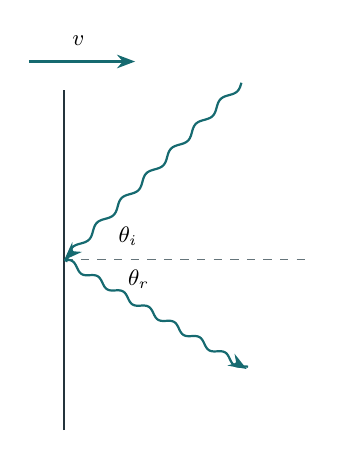
\begin{tikzpicture}[scale=.9,transform shape]
\draw[object] (0.00000,-2.40000)--(0.00000,2.40000);\draw[guide] (0.00000,0.00000)--(3.50000,0.00000);\draw[traj] plot coordinates {(2.50000,2.50000) (2.49214,2.47189) (2.48322,2.44484) (2.47231,2.41977) (2.45867,2.39744) (2.44186,2.37829) (2.42173,2.36244) (2.39853,2.34967) (2.37279,2.33944) (2.34532,2.33094) (2.31710,2.32319) (2.28920,2.31512) (2.26264,2.30571) (2.23832,2.29405) (2.21690,2.27951) (2.19872,2.26171) (2.18382,2.24064) (2.17188,2.21661) (2.16225,2.19027) (2.15408,2.16246) (2.14635,2.13423) (2.13798,2.10662) (2.12799,2.08064) (2.11554,2.05712) (2.10005,2.03664) (2.08127,2.01945) (2.05928,2.00547) (2.03449,1.99429) (2.00761,1.98519) (1.97957,1.97726) (1.95141,1.96945) (1.92419,1.96071) (1.89886,1.95006) (1.87619,1.93676) (1.85667,1.92031) (1.84046,1.90055) (1.82736,1.87767) (1.81688,1.85218) (1.80824,1.82486) (1.80045,1.79667) (1.79247,1.76868) (1.78326,1.74192) (1.77190,1.71731) (1.75770,1.69554) (1.74027,1.67700) (1.71955,1.66174) (1.69584,1.64949) (1.66971,1.63964) (1.64202,1.63136) (1.61378,1.62363) (1.58605,1.61539) (1.55985,1.60562) (1.53602,1.59348) (1.51517,1.57835) (1.49761,1.55994) (1.48329,1.53829) (1.47182,1.51379) (1.46254,1.48710) (1.45453,1.45914) (1.44676,1.43094) (1.43817,1.40356) (1.42778,1.37798) (1.41480,1.35498) (1.39872,1.33510) (1.37933,1.31851) (1.35678,1.30509) (1.33155,1.29435) (1.30438,1.28555) (1.27624,1.27772) (1.24817,1.26981) (1.22123,1.26078) (1.19634,1.24970) (1.17423,1.23585) (1.15531,1.21879) (1.13969,1.19844) (1.12713,1.17503) (1.11705,1.14914) (1.10864,1.12158) (1.10090,1.09334) (1.09277,1.06550) (1.08322,1.03908) (1.07138,1.01495) (1.05661,0.99375) (1.03857,0.97582) (1.01727,0.96114) (0.99306,0.94939) (0.96658,0.93990) (0.93871,0.93179) (0.91048,0.92405) (0.88296,0.91560) (0.85713,0.90546) (0.83382,0.89280) (0.81356,0.87708) (0.79661,0.85807) (0.78285,0.83585) (0.77184,0.81089) (0.76287,0.78390) (0.75498,0.75581) (0.74714,0.72768) (0.73828,0.70056) (0.72747,0.67541) (0.71395,0.65295) (0.69727,0.63367) (0.67728,0.61769) (0.65419,0.60480) (0.62854,0.59448) (0.60112,0.58593) (0.57291,0.57817) (0.54497,0.57014) (0.51834,0.56079) (0.49392,0.54925) (0.47237,0.53483) (0.45406,0.51716) (0.43904,0.49622) (0.42698,0.47230) (0.41728,0.44603) (0.40907,0.41827) (0.40134,0.39003) (0.39302,0.36238) (0.38311,0.33632) (0.37077,0.31269) (0.35541,0.29207) (0.33676,0.27475) (0.31489,0.26065) (0.29021,0.24936) (0.26340,0.24020) (0.23538,0.23224) (0.20721,0.22445) (0.17992,0.21576) (0.15450,0.20521) (0.13172,0.19202) (0.11207,0.17570) (0.09572,0.15608) (0.08251,0.13332) (0.07193,0.10792) (0.06323,0.08065) (0.05544,0.05248) (0.04748,0.02446) (0.03834,-0.00237) (0.02708,-0.02708)};\draw[motion] (0.12728,0.12728)--(0.00000,0.00000);\draw[traj] plot coordinates {(0.00000,0.00000) (0.02587,0.00121) (0.05098,0.00115) (0.07464,-0.00134) (0.09632,-0.00714) (0.11569,-0.01680) (0.13266,-0.03047) (0.14740,-0.04787) (0.16030,-0.06836) (0.17194,-0.09095) (0.18303,-0.11445) (0.19436,-0.13756) (0.20667,-0.15904) (0.22059,-0.17780) (0.23662,-0.19305) (0.25501,-0.20435) (0.27578,-0.21168) (0.29868,-0.21543) (0.32327,-0.21636) (0.34892,-0.21552) (0.37489,-0.21415) (0.40039,-0.21354) (0.42472,-0.21492) (0.44726,-0.21928) (0.46760,-0.22732) (0.48554,-0.23936) (0.50116,-0.25530) (0.51475,-0.27463) (0.52682,-0.29650) (0.53804,-0.31978) (0.54918,-0.34321) (0.56100,-0.36550) (0.57420,-0.38548) (0.58933,-0.40224) (0.60674,-0.41518) (0.62655,-0.42411) (0.64862,-0.42924) (0.67259,-0.43121) (0.69790,-0.43095) (0.72382,-0.42964) (0.74961,-0.42857) (0.77450,-0.42900) (0.79783,-0.43203) (0.81910,-0.43851) (0.83803,-0.44891) (0.85458,-0.46330) (0.86894,-0.48133) (0.88156,-0.50229) (0.89304,-0.52514) (0.90412,-0.54866) (0.91557,-0.57157) (0.92813,-0.59262) (0.94242,-0.61079) (0.95887,-0.62533) (0.97770,-0.63589) (0.99888,-0.64252) (1.02214,-0.64568) (1.04698,-0.64620) (1.07274,-0.64517) (1.09868,-0.64384) (1.12402,-0.64351) (1.14806,-0.64537) (1.17022,-0.65036) (1.19012,-0.65913) (1.20763,-0.67191) (1.22284,-0.68852) (1.23611,-0.70839) (1.24797,-0.73061) (1.25912,-0.75402) (1.27033,-0.77733) (1.28235,-0.79928) (1.29587,-0.81873) (1.31140,-0.83482) (1.32925,-0.84702) (1.34949,-0.85522) (1.37195,-0.85972) (1.39621,-0.86119) (1.42168,-0.86065) (1.44764,-0.85928) (1.47332,-0.85840) (1.49797,-0.85923) (1.52095,-0.86285) (1.54181,-0.87002) (1.56029,-0.88116) (1.57642,-0.89626) (1.59042,-0.91489) (1.60278,-0.93628) (1.61413,-0.95935) (1.62522,-0.98286) (1.63682,-1.00551) (1.64966,-1.02610) (1.66431,-1.04365) (1.68119,-1.05748) (1.70047,-1.06730) (1.72206,-1.07324) (1.74565,-1.07585) (1.77071,-1.07599) (1.79656,-1.07481) (1.82245,-1.07357) (1.84760,-1.07356) (1.87133,-1.07593) (1.89310,-1.08158) (1.91256,-1.09108) (1.92963,-1.10459) (1.94446,-1.12185) (1.95742,-1.14223) (1.96910,-1.16476) (1.98020,-1.18825) (1.99150,-1.21140) (2.00375,-1.23297) (2.01761,-1.25186) (2.03354,-1.26726) (2.05184,-1.27872) (2.07251,-1.28621) (2.09533,-1.29009) (2.11987,-1.29111) (2.14549,-1.29032) (2.17145,-1.28895) (2.19699,-1.28829) (2.22138,-1.28956) (2.24400,-1.29378) (2.26443,-1.30167) (2.28248,-1.31355) (2.29818,-1.32934) (2.31184,-1.34855) (2.32396,-1.37033) (2.33521,-1.39358) (2.34634,-1.41703) (2.35812,-1.43938) (2.37125,-1.45948) (2.38629,-1.47638) (2.40360,-1.48948) (2.42332,-1.49857) (2.44530,-1.50385) (2.46921,-1.50593) (2.49447,-1.50573) (2.52039,-1.50444) (2.54620,-1.50334) (2.57113,-1.50368) (2.59454,-1.50660)};\draw[motion] (2.42040,-1.44710)--(2.57489,-1.53946);\node[above] at (0.90000,0.08000) {$\theta_i$};\node[below] at (1.05000,-0.02000) {$\theta_r$};\draw[motion] (-0.50000,2.80000)--(1.00000,2.80000);\node[above] at (0.20000,2.90000) {$v$};
\end{tikzpicture}
\figcaption{图近2.4\quad 入射从右侧来，两个角从各自规定法线量起。}
\end{minipage}\end{center}

\Needspace{6\baselineskip}\subsection*{解答}


图近2.4将入射角的参考方向定为$-x$，反射角的参考方向定为$+x$。角度都由光的传播方向确定，速度变换使用朝向镜面的实际传播箭头，图中从镜面指向光源的反向线只用于几何定位。

\begin{center}\begin{minipage}{.98\linewidth}\centering
\begin{tikzpicture}[scale=.9,transform shape]
\draw[object] (0.00000,-2.00000)--(0.00000,2.00000);\draw[guide] (0.00000,0.00000)--(3.50000,0.00000);\draw[traj] plot coordinates {(2.38415,1.82094) (2.37569,1.79646) (2.36632,1.77317) (2.35524,1.75212) (2.34182,1.73413) (2.32567,1.71972) (2.30669,1.70902) (2.28506,1.70178) (2.26125,1.69740) (2.23595,1.69496) (2.21002,1.69336) (2.18435,1.69141) (2.15984,1.68794) (2.13725,1.68196) (2.11715,1.67272) (2.09984,1.65983) (2.08533,1.64326) (2.07336,1.62338) (2.06339,1.60088) (2.05466,1.57675) (2.04631,1.55212) (2.03742,1.52821) (2.02713,1.50613) (2.01472,1.48681) (1.99972,1.47090) (1.98188,1.45869) (1.96129,1.45010) (1.93830,1.44464) (1.91351,1.44153) (1.88773,1.43973) (1.86184,1.43807) (1.83676,1.43535) (1.81331,1.43050) (1.79213,1.42267) (1.77366,1.41129) (1.75803,1.39620) (1.74508,1.37760) (1.73437,1.35607) (1.72524,1.33247) (1.71684,1.30790) (1.70828,1.28356) (1.69865,1.26060) (1.68719,1.24006) (1.67329,1.22270) (1.65661,1.20897) (1.63712,1.19894) (1.61504,1.19228) (1.59091,1.18833) (1.56542,1.18613) (1.53947,1.18456) (1.51395,1.18241) (1.48974,1.17855) (1.46758,1.17202) (1.44797,1.16213) (1.43118,1.14855) (1.41717,1.13133) (1.40562,1.11091) (1.39593,1.08803) (1.38734,1.06372) (1.37896,1.03914) (1.36987,1.01548) (1.35924,0.99384) (1.34639,0.97511) (1.33087,0.95987) (1.31251,0.94835) (1.29145,0.94037) (1.26807,0.93542) (1.24304,0.93264) (1.21717,0.93095) (1.19136,0.92918) (1.16652,0.92615) (1.14345,0.92081) (1.12275,0.91235) (1.10480,0.90029) (1.08968,0.88453) (1.07718,0.86534) (1.06682,0.84335) (1.05788,0.81949) (1.04953,0.79487) (1.04083,0.77069) (1.03092,0.74811) (1.01905,0.72810) (1.00465,0.71139) (0.98746,0.69835) (0.96746,0.68897) (0.94496,0.68287) (0.92052,0.67932) (0.89488,0.67733) (0.86894,0.67574) (0.84360,0.67336) (0.81971,0.66907) (0.79799,0.66196) (0.77889,0.65141) (0.76262,0.63715) (0.74910,0.61930) (0.73794,0.59835) (0.72852,0.57513) (0.72003,0.55068) (0.71159,0.52618) (0.70228,0.50281) (0.69128,0.48165) (0.67796,0.46353) (0.66193,0.44897) (0.64305,0.43812) (0.62152,0.43076) (0.59779,0.42627) (0.57254,0.42378) (0.54661,0.42217) (0.52092,0.42025) (0.49634,0.41686) (0.47367,0.41100) (0.45345,0.40191) (0.43603,0.38917) (0.42141,0.37274) (0.40935,0.35298) (0.39931,0.33057) (0.39055,0.30648) (0.38220,0.28185) (0.37335,0.25789) (0.36313,0.23571) (0.35082,0.21627) (0.33592,0.20021) (0.31820,0.18786) (0.29772,0.17912) (0.27481,0.17355) (0.25009,0.17037) (0.22433,0.16854) (0.19842,0.16689) (0.17329,0.16424) (0.14976,0.15950) (0.12849,0.15179) (0.10990,0.14056) (0.09416,0.12562) (0.08110,0.10716) (0.07032,0.08572) (0.06113,0.06219) (0.05273,0.03764) (0.04419,0.01326) (0.03462,-0.00977) (0.02324,-0.03043)};\draw[motion] (0.14305,0.10926)--(0.00000,0.00000);\draw[traj] plot coordinates {(0.00000,0.00000) (0.02584,-0.00172) (0.05078,-0.00463) (0.07401,-0.00978) (0.09489,-0.01799) (0.11304,-0.02978) (0.12836,-0.04528) (0.14104,-0.06424) (0.15153,-0.08606) (0.16054,-0.10982) (0.16891,-0.13442) (0.17755,-0.15867) (0.18734,-0.18140) (0.19906,-0.20162) (0.21326,-0.21859) (0.23025,-0.23190) (0.25005,-0.24153) (0.27239,-0.24785) (0.29671,-0.25155) (0.32229,-0.25362) (0.34825,-0.25519) (0.37366,-0.25748) (0.39767,-0.26160) (0.41957,-0.26848) (0.43887,-0.27877) (0.45534,-0.29277) (0.46905,-0.31037) (0.48036,-0.33112) (0.48988,-0.35421) (0.49840,-0.37861) (0.50682,-0.40315) (0.51604,-0.42663) (0.52689,-0.44798) (0.54003,-0.46634) (0.55586,-0.48117) (0.57453,-0.49228) (0.59588,-0.49988) (0.61948,-0.50455) (0.64465,-0.50715) (0.67056,-0.50878) (0.69630,-0.51064) (0.72098,-0.51388) (0.74382,-0.51954) (0.76422,-0.52838) (0.78185,-0.54086) (0.79666,-0.55702) (0.80889,-0.57657) (0.81906,-0.59882) (0.82788,-0.62282) (0.83623,-0.64745) (0.84502,-0.67150) (0.85511,-0.69384) (0.86725,-0.71351) (0.88195,-0.72982) (0.89946,-0.74244) (0.91976,-0.75143) (0.94251,-0.75720) (0.96713,-0.76052) (0.99284,-0.76241) (1.01877,-0.76403) (1.04398,-0.76657) (1.06765,-0.77113) (1.08911,-0.77860) (1.10789,-0.78957) (1.12384,-0.80424) (1.13708,-0.82247) (1.14801,-0.84372) (1.15728,-0.86713) (1.16571,-0.89165) (1.17421,-0.91608) (1.18367,-0.93925) (1.19490,-0.96011) (1.20851,-0.97785) (1.22486,-0.99199) (1.24405,-1.00243) (1.26585,-1.00944) (1.28979,-1.01365) (1.31516,-1.01599) (1.34111,-1.01758) (1.36672,-1.01960) (1.39112,-1.02322) (1.41355,-1.02941) (1.43346,-1.03890) (1.45056,-1.05206) (1.46487,-1.06888) (1.47668,-1.08898) (1.48654,-1.11163) (1.49521,-1.13584) (1.50357,-1.16045) (1.51253,-1.18427) (1.52295,-1.20618) (1.53553,-1.22528) (1.55074,-1.24092) (1.56877,-1.25286) (1.58955,-1.26121) (1.61270,-1.26647) (1.63758,-1.26945) (1.66340,-1.27120) (1.68926,-1.27290) (1.71425,-1.27573) (1.73756,-1.28077) (1.75855,-1.28885) (1.77682,-1.30049) (1.79225,-1.31584) (1.80502,-1.33468) (1.81559,-1.35639) (1.82465,-1.38010) (1.83302,-1.40469) (1.84163,-1.42897) (1.85137,-1.45179) (1.86299,-1.47212) (1.87708,-1.48923) (1.89396,-1.50269) (1.91365,-1.51247) (1.93589,-1.51890) (1.96016,-1.52269) (1.98570,-1.52481) (2.01166,-1.52638) (2.03711,-1.52862) (2.06119,-1.53264) (2.08319,-1.53940) (2.10260,-1.54954) (2.11918,-1.56339) (2.13300,-1.58085) (2.14440,-1.60149) (2.15398,-1.62450) (2.16252,-1.64887) (2.17092,-1.67343) (2.18010,-1.69698) (2.19087,-1.71843) (2.20390,-1.73693) (2.21962,-1.75190) (2.23818,-1.76316) (2.25943,-1.77089) (2.28294,-1.77566) (2.30807,-1.77833) (2.33396,-1.77998) (2.35973,-1.78180) (2.38447,-1.78497) (2.40739,-1.79051)};\draw[motion] (2.24110,-1.71168)--(2.38415,-1.82094);\node[above] at (0.90000,0.08000) {$\theta_0$};\node[below] at (0.90000,-0.08000) {$\theta_0$};\node[above] at (1.50000,2.80000) {镜系：等角、同频};
\end{tikzpicture}
\figcaption{解图近2.4A\quad 先在镜面静止系使用普通反射定律。}
\end{minipage}\end{center}
解图近2.4A为镜面静止系$S'$。设入射与反射角均为$\theta_0$，镜系的反射定律为$\theta_i'=\theta_r'=\theta_0$。记$\gamma=(1-\beta^2)^{-1/2}$。由光行差公式，
\[
\frac{u_x'}c=\frac{u_x/c-\beta}{1-\beta u_x/c},
\qquad
\frac{u_y'}c=\frac{u_y/c}{\gamma(1-\beta u_x/c)}.
\]
入射光$u_x/c=-\cos\theta_i$，所以
\[
\cos\theta_0=\frac{\cos\theta_i+\beta}{1+\beta\cos\theta_i},
\qquad
\sin\theta_0=\frac{\sin\theta_i}{\gamma(1+\beta\cos\theta_i)}.
\]
入射能撞向镜面，要求镜系入射法向分量朝向镜面，即
\[
\boxed{\cos\theta_i+\beta>0}.
\]
图C以光线与镜面世界线的交点表示这个相遇条件。负$v$退行镜的速率范围由这一条件选定；超过该范围时，光与镜面的初始间隔随时间保持或增大。
\begin{center}\begin{minipage}{.98\linewidth}\centering
\begin{tikzpicture}[scale=.8,transform shape]
\draw[axis] (0,0)--(8,0) node[right] {$ct$};
\draw[axis] (0,-3)--(0,3) node[above] {$x$};
\draw[guide] (0,0)--(6,-1.8);
\draw[traj] (0,1)--(6,-2);
\draw[guide] (6,-1.8)--(6.48,-1.15) node[right] {镜面$x=-0.3ct$};
\draw[guide] (6,-2)--(6.48,-2.49) node[right] {入射$x=\ell-0.5ct$};
\node[left] at (0,1) {$\ell$};
\fill (5,-1.5) circle(.04) node[left] {相交};
\end{tikzpicture}
\figcaption{解图近2.4C\quad 示例入射60度、镜速$-0.3c$，两条世界线求交}
\end{minipage}\end{center}

反射光在镜系法向分量为$+c\cos\theta_0$。变回$S$，有
\[
\cos\theta_0=\frac{\cos\theta_r-\beta}{1-\beta\cos\theta_r},
\qquad
\sin\theta_0=\frac{\sin\theta_r}{\gamma(1-\beta\cos\theta_r)}.
\]
消去镜系角，得到两种等价关系
\[
\boxed{\frac{\cos\theta_i+\beta}{1+\beta\cos\theta_i}
=\frac{\cos\theta_r-\beta}{1-\beta\cos\theta_r}},
\]
\[
\boxed{\frac{\sin\theta_i}{1+\beta\cos\theta_i}
=\frac{\sin\theta_r}{1-\beta\cos\theta_r}}.
\]
后一式与余弦关系共同确定法向分量符号，分别选出锐角或钝角反射支。

\begin{center}\begin{minipage}{.98\linewidth}\centering
\begin{tikzpicture}[scale=.88,transform shape]
\draw[object] (0.00000,-2.80000)--(0.00000,2.80000);\draw[guide] (0.00000,0.00000)--(3.50000,0.00000);\draw[traj] plot coordinates {(2.50000,2.50000) (2.49214,2.47189) (2.48322,2.44484) (2.47231,2.41977) (2.45867,2.39744) (2.44186,2.37829) (2.42173,2.36244) (2.39853,2.34967) (2.37279,2.33944) (2.34532,2.33094) (2.31710,2.32319) (2.28920,2.31512) (2.26264,2.30571) (2.23832,2.29405) (2.21690,2.27951) (2.19872,2.26171) (2.18382,2.24064) (2.17188,2.21661) (2.16225,2.19027) (2.15408,2.16246) (2.14635,2.13423) (2.13798,2.10662) (2.12799,2.08064) (2.11554,2.05712) (2.10005,2.03664) (2.08127,2.01945) (2.05928,2.00547) (2.03449,1.99429) (2.00761,1.98519) (1.97957,1.97726) (1.95141,1.96945) (1.92419,1.96071) (1.89886,1.95006) (1.87619,1.93676) (1.85667,1.92031) (1.84046,1.90055) (1.82736,1.87767) (1.81688,1.85218) (1.80824,1.82486) (1.80045,1.79667) (1.79247,1.76868) (1.78326,1.74192) (1.77190,1.71731) (1.75770,1.69554) (1.74027,1.67700) (1.71955,1.66174) (1.69584,1.64949) (1.66971,1.63964) (1.64202,1.63136) (1.61378,1.62363) (1.58605,1.61539) (1.55985,1.60562) (1.53602,1.59348) (1.51517,1.57835) (1.49761,1.55994) (1.48329,1.53829) (1.47182,1.51379) (1.46254,1.48710) (1.45453,1.45914) (1.44676,1.43094) (1.43817,1.40356) (1.42778,1.37798) (1.41480,1.35498) (1.39872,1.33510) (1.37933,1.31851) (1.35678,1.30509) (1.33155,1.29435) (1.30438,1.28555) (1.27624,1.27772) (1.24817,1.26981) (1.22123,1.26078) (1.19634,1.24970) (1.17423,1.23585) (1.15531,1.21879) (1.13969,1.19844) (1.12713,1.17503) (1.11705,1.14914) (1.10864,1.12158) (1.10090,1.09334) (1.09277,1.06550) (1.08322,1.03908) (1.07138,1.01495) (1.05661,0.99375) (1.03857,0.97582) (1.01727,0.96114) (0.99306,0.94939) (0.96658,0.93990) (0.93871,0.93179) (0.91048,0.92405) (0.88296,0.91560) (0.85713,0.90546) (0.83382,0.89280) (0.81356,0.87708) (0.79661,0.85807) (0.78285,0.83585) (0.77184,0.81089) (0.76287,0.78390) (0.75498,0.75581) (0.74714,0.72768) (0.73828,0.70056) (0.72747,0.67541) (0.71395,0.65295) (0.69727,0.63367) (0.67728,0.61769) (0.65419,0.60480) (0.62854,0.59448) (0.60112,0.58593) (0.57291,0.57817) (0.54497,0.57014) (0.51834,0.56079) (0.49392,0.54925) (0.47237,0.53483) (0.45406,0.51716) (0.43904,0.49622) (0.42698,0.47230) (0.41728,0.44603) (0.40907,0.41827) (0.40134,0.39003) (0.39302,0.36238) (0.38311,0.33632) (0.37077,0.31269) (0.35541,0.29207) (0.33676,0.27475) (0.31489,0.26065) (0.29021,0.24936) (0.26340,0.24020) (0.23538,0.23224) (0.20721,0.22445) (0.17992,0.21576) (0.15450,0.20521) (0.13172,0.19202) (0.11207,0.17570) (0.09572,0.15608) (0.08251,0.13332) (0.07193,0.10792) (0.06323,0.08065) (0.05544,0.05248) (0.04748,0.02446) (0.03834,-0.00237) (0.02708,-0.02708)};\draw[motion] (0.12728,0.12728)--(0.00000,0.00000);\draw[motion] (0.00000,0.00000)--(2.57489,-1.53946);\node[right] at (2.57489,-1.53946) {$\beta=0.2$};\draw[force] (0.00000,0.00000)--(-0.64165,-2.93058);\node[below left] at (-0.64165,-2.93058) {$\beta=-0.5$};\node[above] at (1.70000,2.80000) {同一入射角45°};\node[below] at (1.50000,-3.50000) {退行支用相对镜面的法向速度判定};
\end{tikzpicture}
\figcaption{解图近2.4B\quad 迎光反射角变小，退行反射可进入钝角支。}
\end{minipage}\end{center}
法向、横向分量比还给出不含频率的切线形式。入射与反射在镜系的同一锐角满足$\tan\theta_0=\sin\theta_i/[\gamma(\cos\theta_i+\beta)]=\sin\theta_r/[\gamma(\cos\theta_r-\beta)]$，因此$\sin\theta_i/(\cos\theta_i+\beta)=\sin\theta_r/(\cos\theta_r-\beta)$。该式与余弦、正弦两式从同一二维速度变换导出；当反射法向分量跨零时，继续保留两个分量的符号便得到连续的钝角支。

令$D=1+\beta^2+2\beta\cos\theta_i$。解图近2.4B的实验室两条出射线按下式确定：
\[
\boxed{\cos\theta_r=\frac{(1+\beta^2)\cos\theta_i+2\beta}{D}},
\qquad
\boxed{\sin\theta_r=\frac{(1-\beta^2)\sin\theta_i}{D}}.
\]
由$D\ge(1-|\beta|)^2>0$，上述两个分量具有确定的符号。取$\theta_r=\operatorname{atan2}(\sin\theta_r,\cos\theta_r)$，正弦非负给出$0\le\theta_r\le\pi$的唯一连续方向，余弦正、零、负分别对应锐角、直角和钝角。

当$\beta=0$，立即恢复$\theta_r=\theta_i$。对允许发生碰撞的光线，
\[
\cos\theta_r-\cos\theta_i
=\frac{2\beta\sin^2\theta_i}{D}.
\]
所以非正入射时，$\beta>0$表示镜面迎着入射光运动，有$\theta_r<\theta_i$；$\beta<0$表示镜面沿入射的法向分量退行，有$\theta_r>\theta_i$。退行足够快时，反射光的实验室法向分量甚至仍为负，但它比镜面退得慢，仍然与镜面分离。判别分离应看$\cos\theta_r-\beta>0$，由光与镜面的相对法向速度判定。

同一镜系反射还给出频率与机械功的联系。两次洛伦兹变换、镜系弹性反射给
\[
\nu_i'=\gamma\nu_i(1+\beta\cos\theta_i),\qquad
\nu_r=\gamma\nu_i'(1+\beta\cos\theta_0),
\]
\[
\frac{\nu_r}{\nu_i}=\frac{D}{1-\beta^2}.
\]
图D把频率比画成镜速的函数：迎面镜反射蓝移，退行镜反射红移，分别对应光从镜面系统取得能量和向它交付能量。
\begin{center}\begin{minipage}{.98\linewidth}\centering
\begin{tikzpicture}[scale=.8,transform shape]
\draw[axis] (0,0)--(10.7,0) node[right] {$\beta$};
\draw[axis] (0,0)--(0,3.2) node[above] {$\nu_r/\nu_i$};
\node[above] at (5,3.5) {入射45度的频率比；负速率段取可碰撞支};
\draw[traj] plot coordinates {(0.000000000,0.435723969) (0.055555556,0.429538742) (0.111111111,0.423708885) (0.166666667,0.418215119) (0.222222222,0.413039660) (0.277777778,0.408166080) (0.333333333,0.403579185) (0.388888889,0.399264900) (0.444444444,0.395210173) (0.500000000,0.391402885) (0.555555556,0.387831776) (0.611111111,0.384486365) (0.666666667,0.381356894) (0.722222222,0.378434263) (0.777777778,0.375709983) (0.833333333,0.373176128) (0.888888889,0.370825289) (0.944444444,0.368650536) (1.000000000,0.366645386) (1.055555556,0.364803766) (1.111111111,0.363119985) (1.166666667,0.361588710) (1.222222222,0.360204938) (1.277777778,0.358963974) (1.333333333,0.357861412) (1.388888889,0.356893115) (1.444444444,0.356055197) (1.500000000,0.355344008) (1.555555556,0.354756120) (1.611111111,0.354288312) (1.666666667,0.353937559) (1.722222222,0.353701017) (1.777777778,0.353576019) (1.833333333,0.353560057) (1.888888889,0.353650781) (1.944444444,0.353845983) (2.000000000,0.354143596) (2.055555556,0.354541683) (2.111111111,0.355038429) (2.166666667,0.355632139) (2.222222222,0.356321230) (2.277777778,0.357104225) (2.333333333,0.357979749) (2.388888889,0.358946524) (2.444444444,0.360003366) (2.500000000,0.361149178) (2.555555556,0.362382951) (2.611111111,0.363703756) (2.666666667,0.365110744) (2.722222222,0.366603140) (2.777777778,0.368180244) (2.833333333,0.369841426) (2.888888889,0.371586124) (2.944444444,0.373413842) (3.000000000,0.375324149) (3.055555556,0.377316676) (3.111111111,0.379391114) (3.166666667,0.381547214) (3.222222222,0.383784785) (3.277777778,0.386103690) (3.333333333,0.388503850) (3.388888889,0.390985241) (3.444444444,0.393547888) (3.500000000,0.396191874) (3.555555556,0.398917329) (3.611111111,0.401724437) (3.666666667,0.404613433) (3.722222222,0.407584599) (3.777777778,0.410638271) (3.833333333,0.413774831) (3.888888889,0.416994713) (3.944444444,0.420298398) (4.000000000,0.423686419) (4.055555556,0.427159356) (4.111111111,0.430717839) (4.166666667,0.434362548) (4.222222222,0.438094213) (4.277777778,0.441913615) (4.333333333,0.445821583) (4.388888889,0.449819001) (4.444444444,0.453906802) (4.500000000,0.458085972) (4.555555556,0.462357552) (4.611111111,0.466722636) (4.666666667,0.471182371) (4.722222222,0.475737963) (4.777777778,0.480390673) (4.833333333,0.485141822) (4.888888889,0.489992789) (4.944444444,0.494945015) (5.000000000,0.500000000) (5.055555556,0.505159312) (5.111111111,0.510424582) (5.166666667,0.515797507) (5.222222222,0.521279857) (5.277777778,0.526873467) (5.333333333,0.532580250) (5.388888889,0.538402191) (5.444444444,0.544341354) (5.500000000,0.550399880) (5.555555556,0.556579997) (5.611111111,0.562884013) (5.666666667,0.569314326) (5.722222222,0.575873427) (5.777777778,0.582563898) (5.833333333,0.589388418) (5.888888889,0.596349770) (5.944444444,0.603450840) (6.000000000,0.610694621) (6.055555556,0.618084221) (6.111111111,0.625622864) (6.166666667,0.633313896) (6.222222222,0.641160790) (6.277777778,0.649167149) (6.333333333,0.657336714) (6.388888889,0.665673369) (6.444444444,0.674181147) (6.500000000,0.682864235) (6.555555556,0.691726982) (6.611111111,0.700773906) (6.666666667,0.710009703) (6.722222222,0.719439249) (6.777777778,0.729067618) (6.833333333,0.738900082) (6.888888889,0.748942125) (6.944444444,0.759199451) (7.000000000,0.769677996) (7.055555556,0.780383938) (7.111111111,0.791323711) (7.166666667,0.802504013) (7.222222222,0.813931825) (7.277777778,0.825614420) (7.333333333,0.837559382) (7.388888889,0.849774619) (7.444444444,0.862268383) (7.500000000,0.875049285) (7.555555556,0.888126315) (7.611111111,0.901508867) (7.666666667,0.915206754) (7.722222222,0.929230234) (7.777777778,0.943590039) (7.833333333,0.958297395) (7.888888889,0.973364057) (7.944444444,0.988802334) (8.000000000,1.004625126) (8.055555556,1.020845957) (8.111111111,1.037479013) (8.166666667,1.054539183) (8.222222222,1.072042102) (8.277777778,1.090004198) (8.333333333,1.108442742) (8.388888889,1.127375904) (8.444444444,1.146822809) (8.500000000,1.166803601) (8.555555556,1.187339513) (8.611111111,1.208452940) (8.666666667,1.230167516) (8.722222222,1.252508207) (8.777777778,1.275501398) (8.833333333,1.299175003) (8.888888889,1.323558567) (8.944444444,1.348683396) (9.000000000,1.374582684) (9.055555556,1.401291658) (9.111111111,1.428847737) (9.166666667,1.457290702) (9.222222222,1.486662888) (9.277777778,1.517009390) (9.333333333,1.548378291) (9.388888889,1.580820912) (9.444444444,1.614392093) (9.500000000,1.649150495) (9.555555556,1.685158939) (9.611111111,1.722484783) (9.666666667,1.761200335) (9.722222222,1.801383320) (9.777777778,1.843117392) (9.833333333,1.886492713) (9.888888889,1.931606597) (9.944444444,1.978564233) (10.000000000,2.027479494)};
\node[below] at (0,-.12) {$-0.65$};
\node[below] at (5,-.12) {$0$};
\node[below] at (10,-.12) {$0.65$};
\end{tikzpicture}
\figcaption{解图近2.4D\quad 入射45度的频率比；负速率段取可碰撞支}
\end{minipage}\end{center}给定的匀速镜速由维持机构保持，反射中的能量交换按上述频移计算。


\Needspace{13\baselineskip}

\pdfbookmark[2]{第 5 题 共同运动的介质界面}{q5}

\section*{第 5 题\quad 共同运动的介质界面}\label{q:5}

两种均匀、透明、各向同性且无色散的介质与它们的平面界面共同以$v=\beta c$沿实验室系$S$的$+x$运动，$0\le\beta<1$，界面法线为$x$轴。两介质在共同静止系$S'$的折射率为$n_1,n_2\ge1$。光从介质1射向介质2；在$S$中，入射角$\theta_i$从$+x$量起，反射角$\theta_r$从$-x$量起，折射角$\theta_t$从$+x$量起，均取图示正横向分量。

求实验室中反射角、折射角与入射角的关系，说明传播分支与适用角域；再给出介质1为真空、介质2折射率为$n$时的结果。只讨论能射到界面的入射支；若发生全反射，应指出没有传播折射光。

\begin{center}\begin{minipage}{.98\linewidth}\centering
\begin{tikzpicture}[scale=.9,transform shape]
\draw[object] (0.00000,-2.80000)--(0.00000,2.80000);\draw[guide] (-3.20000,0.00000)--(3.80000,0.00000);\draw[traj] plot coordinates {(-2.38415,-1.82094) (-2.37569,-1.79646) (-2.36632,-1.77317) (-2.35524,-1.75212) (-2.34182,-1.73413) (-2.32567,-1.71972) (-2.30669,-1.70902) (-2.28506,-1.70178) (-2.26125,-1.69740) (-2.23595,-1.69496) (-2.21002,-1.69336) (-2.18435,-1.69141) (-2.15984,-1.68794) (-2.13725,-1.68196) (-2.11715,-1.67272) (-2.09984,-1.65983) (-2.08533,-1.64326) (-2.07336,-1.62338) (-2.06339,-1.60088) (-2.05466,-1.57675) (-2.04631,-1.55212) (-2.03742,-1.52821) (-2.02713,-1.50613) (-2.01472,-1.48681) (-1.99972,-1.47090) (-1.98188,-1.45869) (-1.96129,-1.45010) (-1.93830,-1.44464) (-1.91351,-1.44153) (-1.88773,-1.43973) (-1.86184,-1.43807) (-1.83676,-1.43535) (-1.81331,-1.43050) (-1.79213,-1.42267) (-1.77366,-1.41129) (-1.75803,-1.39620) (-1.74508,-1.37760) (-1.73437,-1.35607) (-1.72524,-1.33247) (-1.71684,-1.30790) (-1.70828,-1.28356) (-1.69865,-1.26060) (-1.68719,-1.24006) (-1.67329,-1.22270) (-1.65661,-1.20897) (-1.63712,-1.19894) (-1.61504,-1.19228) (-1.59091,-1.18833) (-1.56542,-1.18613) (-1.53947,-1.18456) (-1.51395,-1.18241) (-1.48974,-1.17855) (-1.46758,-1.17202) (-1.44797,-1.16213) (-1.43118,-1.14855) (-1.41717,-1.13133) (-1.40562,-1.11091) (-1.39593,-1.08803) (-1.38734,-1.06372) (-1.37896,-1.03914) (-1.36987,-1.01548) (-1.35924,-0.99384) (-1.34639,-0.97511) (-1.33087,-0.95987) (-1.31251,-0.94835) (-1.29145,-0.94037) (-1.26807,-0.93542) (-1.24304,-0.93264) (-1.21717,-0.93095) (-1.19136,-0.92918) (-1.16652,-0.92615) (-1.14345,-0.92081) (-1.12275,-0.91235) (-1.10480,-0.90029) (-1.08968,-0.88453) (-1.07718,-0.86534) (-1.06682,-0.84335) (-1.05788,-0.81949) (-1.04953,-0.79487) (-1.04083,-0.77069) (-1.03092,-0.74811) (-1.01905,-0.72810) (-1.00465,-0.71139) (-0.98746,-0.69835) (-0.96746,-0.68897) (-0.94496,-0.68287) (-0.92052,-0.67932) (-0.89488,-0.67733) (-0.86894,-0.67574) (-0.84360,-0.67336) (-0.81971,-0.66907) (-0.79799,-0.66196) (-0.77889,-0.65141) (-0.76262,-0.63715) (-0.74910,-0.61930) (-0.73794,-0.59835) (-0.72852,-0.57513) (-0.72003,-0.55068) (-0.71159,-0.52618) (-0.70228,-0.50281) (-0.69128,-0.48165) (-0.67796,-0.46353) (-0.66193,-0.44897) (-0.64305,-0.43812) (-0.62152,-0.43076) (-0.59779,-0.42627) (-0.57254,-0.42378) (-0.54661,-0.42217) (-0.52092,-0.42025) (-0.49634,-0.41686) (-0.47367,-0.41100) (-0.45345,-0.40191) (-0.43603,-0.38917) (-0.42141,-0.37274) (-0.40935,-0.35298) (-0.39931,-0.33057) (-0.39055,-0.30648) (-0.38220,-0.28185) (-0.37335,-0.25789) (-0.36313,-0.23571) (-0.35082,-0.21627) (-0.33592,-0.20021) (-0.31820,-0.18786) (-0.29772,-0.17912) (-0.27481,-0.17355) (-0.25009,-0.17037) (-0.22433,-0.16854) (-0.19842,-0.16689) (-0.17329,-0.16424) (-0.14976,-0.15950) (-0.12849,-0.15179) (-0.10990,-0.14056) (-0.09416,-0.12562) (-0.08110,-0.10716) (-0.07032,-0.08572) (-0.06113,-0.06219) (-0.05273,-0.03764) (-0.04419,-0.01326) (-0.03462,0.00977) (-0.02324,0.03043)};\draw[motion] (-0.14305,-0.10926)--(0.00000,0.00000);\draw[traj] plot coordinates {(0.00000,0.00000) (-0.02430,0.00896) (-0.04740,0.01880) (-0.06822,0.03031) (-0.08593,0.04409) (-0.10001,0.06053) (-0.11032,0.07973) (-0.11711,0.10150) (-0.12101,0.12540) (-0.12293,0.15074) (-0.12400,0.17670) (-0.12543,0.20240) (-0.12840,0.22698) (-0.13392,0.24968) (-0.14274,0.26997) (-0.15528,0.28754) (-0.17154,0.30238) (-0.19118,0.31476) (-0.21347,0.32519) (-0.23742,0.33440) (-0.26187,0.34326) (-0.28559,0.35264) (-0.30746,0.36337) (-0.32653,0.37617) (-0.34212,0.39150) (-0.35396,0.40958) (-0.36214,0.43034) (-0.36712,0.45344) (-0.36972,0.47828) (-0.37100,0.50410) (-0.37213,0.53001) (-0.37434,0.55515) (-0.37871,0.57869) (-0.38611,0.60002) (-0.39711,0.61872) (-0.41187,0.63466) (-0.43020,0.64799) (-0.45152,0.65913) (-0.47492,0.66875) (-0.49931,0.67764) (-0.52348,0.68670) (-0.54624,0.69679) (-0.56654,0.70867) (-0.58361,0.72293) (-0.59699,0.73988) (-0.60663,0.75957) (-0.61283,0.78178) (-0.61629,0.80599) (-0.61797,0.83151) (-0.61901,0.85749) (-0.62064,0.88305) (-0.62400,0.90733) (-0.63008,0.92963) (-0.63957,0.94943) (-0.65280,0.96649) (-0.66973,0.98085) (-0.68992,0.99282) (-0.71259,1.00297) (-0.73672,1.01205) (-0.76113,1.02094) (-0.78460,1.03050) (-0.80601,1.04158) (-0.82448,1.05481) (-0.83940,1.07063) (-0.85054,1.08922) (-0.85808,1.11045) (-0.86256,1.13392) (-0.86483,1.15900) (-0.86599,1.18490) (-0.86723,1.21074) (-0.86976,1.23564) (-0.87463,1.25882) (-0.88266,1.27968) (-0.89435,1.29788) (-0.90980,1.31331) (-0.92873,1.32620) (-0.95050,1.33701) (-0.97418,1.34643) (-0.99862,1.35529) (-1.02261,1.36447) (-1.04499,1.37484) (-1.06475,1.38712) (-1.08116,1.40185) (-1.09385,1.41931) (-1.10282,1.43950) (-1.10846,1.46212) (-1.11151,1.48663) (-1.11298,1.51230) (-1.11404,1.53827) (-1.11590,1.56365) (-1.11970,1.58762) (-1.12637,1.60949) (-1.13653,1.62880) (-1.15045,1.64535) (-1.16802,1.65924) (-1.18874,1.67082) (-1.21176,1.68071) (-1.23604,1.68969) (-1.26036,1.69864) (-1.28353,1.70842) (-1.30446,1.71985) (-1.32231,1.73353) (-1.33654,1.74986) (-1.34700,1.76895) (-1.35392,1.79063) (-1.35792,1.81445) (-1.35990,1.83975) (-1.36098,1.86570) (-1.36237,1.89143) (-1.36526,1.91607) (-1.37066,1.93886) (-1.37934,1.95925) (-1.39172,1.97694) (-1.40784,1.99188) (-1.42736,2.00435) (-1.44956,2.01484) (-1.47346,2.02409) (-1.49791,2.03294) (-1.52169,2.04228) (-1.54365,2.05295) (-1.56284,2.06566) (-1.57859,2.08088) (-1.59058,2.09885) (-1.59890,2.11951) (-1.60400,2.14252) (-1.60668,2.16731) (-1.60798,2.19310) (-1.60910,2.21903) (-1.61124,2.24421) (-1.61550,2.26783) (-1.62277,2.28926) (-1.63361,2.30807) (-1.64823,2.32411) (-1.66643,2.33754) (-1.68763,2.34877) (-1.71098,2.35843) (-1.73535,2.36733) (-1.75955,2.37637) (-1.78238,2.38640) (-1.80280,2.39820)};\draw[motion] (-1.66559,2.27557)--(-1.77191,2.42082);\draw[traj] plot coordinates {(0.00000,0.00000) (0.01489,0.02119) (0.03032,0.04099) (0.04678,0.05817) (0.06465,0.07175) (0.08415,0.08114) (0.10535,0.08619) (0.12814,0.08717) (0.15223,0.08481) (0.17722,0.08017) (0.20259,0.07455) (0.22780,0.06934) (0.25231,0.06591) (0.27567,0.06542) (0.29755,0.06874) (0.31774,0.07636) (0.33626,0.08828) (0.35325,0.10408) (0.36905,0.12295) (0.38410,0.14374) (0.39893,0.16510) (0.41408,0.18563) (0.43006,0.20401) (0.44732,0.21916) (0.46613,0.23030) (0.48665,0.23711) (0.50881,0.23969) (0.53241,0.23858) (0.55709,0.23473) (0.58237,0.22934) (0.60771,0.22379) (0.63257,0.21948) (0.65645,0.21766) (0.67896,0.21935) (0.69986,0.22519) (0.71905,0.23537) (0.73663,0.24967) (0.75287,0.26742) (0.76816,0.28757) (0.78301,0.30887) (0.79797,0.32990) (0.81355,0.34931) (0.83025,0.36589) (0.84840,0.37873) (0.86822,0.38732) (0.88972,0.39159) (0.91278,0.39189) (0.93707,0.38902) (0.96216,0.38410) (0.98755,0.37845) (1.01266,0.37347) (1.03700,0.37049) (1.06011,0.37065) (1.08168,0.37475) (1.10157,0.38316) (1.11978,0.39584) (1.13653,0.41228) (1.15215,0.43160) (1.16712,0.45259) (1.18196,0.47391) (1.19723,0.49414) (1.21342,0.51200) (1.23095,0.52645) (1.25007,0.53681) (1.27089,0.54282) (1.29334,0.54467) (1.31718,0.54298) (1.34200,0.53874) (1.36734,0.53322) (1.39263,0.52779) (1.41734,0.52385) (1.44100,0.52262) (1.46322,0.52503) (1.48380,0.53166) (1.50269,0.54264) (1.52000,0.55763) (1.53603,0.57591) (1.55120,0.59637) (1.56603,0.61773) (1.58106,0.63856) (1.59682,0.65753) (1.61376,0.67348) (1.63221,0.68557) (1.65234,0.69336) (1.67414,0.69685) (1.69745,0.69650) (1.72193,0.69317) (1.74712,0.68800) (1.77249,0.68237) (1.79750,0.67766) (1.82164,0.67519) (1.84449,0.67602) (1.86576,0.68089) (1.88533,0.69011) (1.90326,0.70353) (1.91977,0.72058) (1.93523,0.74030) (1.95013,0.76146) (1.96502,0.78268) (1.98042,0.80256) (1.99683,0.81987) (2.01463,0.83361) (2.03406,0.84317) (2.05520,0.84839) (2.07793,0.84953) (2.10197,0.84728) (2.12693,0.84271) (2.15230,0.83710) (2.17752,0.83185) (2.20207,0.82832) (2.22549,0.82769) (2.24743,0.83085) (2.26769,0.83829) (2.28627,0.85004) (2.30333,0.86570) (2.31916,0.88447) (2.33423,0.90520) (2.34906,0.92657) (2.36418,0.94716) (2.38013,0.96565) (2.39732,0.98094) (2.41607,0.99226) (2.43652,0.99924) (2.45862,1.00198) (2.48217,1.00101) (2.50681,0.99725) (2.53208,0.99189) (2.55743,0.98632) (2.58231,0.98193) (2.60624,0.98000) (2.62882,0.98153) (2.64978,0.98719) (2.66904,0.99720) (2.68668,1.01135) (2.70297,1.02897) (2.71829,1.04905) (2.73315,1.07033) (2.74809,1.09140) (2.76364,1.11090) (2.78028,1.12761)};\draw[motion] (2.62656,1.02643)--(2.79422,1.09195);\node[above] at (-2.00000,2.80000) {介质1};\node[above] at (2.00000,2.80000) {介质2};\node[below] at (-1.10000,-0.04000) {$\theta_i$};\node[above] at (-1.05000,0.06000) {$\theta_r$};\node[below] at (1.65000,-0.04000) {$\theta_t$};\draw[motion] (-0.50000,3.50000)--(1.00000,3.50000);\node[above] at (0.25000,3.60000) {$v$};
\end{tikzpicture}
\figcaption{图近2.5\quad 界面和两介质共同移动，三角均按传播方向定义。}
\end{minipage}\end{center}

\Needspace{6\baselineskip}\subsection*{解答}


图近2.5中，折射率是在介质静止系定义的。运动介质中的实验室光速由静止介质光速$c/n_j$作速度变换得到。记$\gamma=(1-\beta^2)^{-1/2}$，静止界面系入射角为$\psi$，则
\[
0\le\psi<\frac\pi2,\qquad
\theta_r'=\psi,\qquad n_1\sin\psi=n_2\sin\psi_t.
\]
解图近2.5A先在$S'$作普通反射、折射，再将三支传播速度分别变回$S$。两种介质在 $S'$ 中均匀、各向同性且无色散。这个系里群速度与相速度同向，光线的传播速率为 $c/n_j$。实验室图跟踪光线到达界面后的方向，因此对群速度的两个分量作变换。下面分别变换三支实际传播速度，得到实验室中的光线方向。

\begin{center}\begin{minipage}{.98\linewidth}\centering
\begin{tikzpicture}[scale=.85,transform shape]
\draw[object] (0.00000,-2.80000)--(0.00000,2.80000);\draw[guide] (-3.20000,0.00000)--(3.80000,0.00000);\draw[traj] plot coordinates {(-2.12132,-2.12132) (-2.11618,-2.09594) (-2.10999,-2.07160) (-2.10181,-2.04927) (-2.09089,-2.02966) (-2.07680,-2.01323) (-2.05940,-2.00011) (-2.03892,-1.99006) (-2.01591,-1.98255) (-1.99116,-1.97678) (-1.96566,-1.97175) (-1.94048,-1.96641) (-1.91665,-1.95972) (-1.89506,-1.95079) (-1.87636,-1.93897) (-1.86091,-1.92389) (-1.84873,-1.90555) (-1.83951,-1.88425) (-1.83261,-1.86062) (-1.82716,-1.83555) (-1.82215,-1.81003) (-1.81652,-1.78515) (-1.80925,-1.76190) (-1.79952,-1.74110) (-1.78676,-1.72334) (-1.77070,-1.70888) (-1.75143,-1.69762) (-1.72937,-1.68916) (-1.70521,-1.68279) (-1.67990,-1.67759) (-1.65446,-1.67250) (-1.62996,-1.66648) (-1.60736,-1.65856) (-1.58742,-1.64798) (-1.57062,-1.63425) (-1.55713,-1.61722) (-1.54676,-1.59707) (-1.53900,-1.57430) (-1.53308,-1.54970) (-1.52802,-1.52424) (-1.52277,-1.49897) (-1.51628,-1.47494) (-1.50764,-1.45305) (-1.49616,-1.43401) (-1.48146,-1.41819) (-1.46347,-1.40565) (-1.44248,-1.39613) (-1.41907,-1.38900) (-1.39411,-1.38345) (-1.36859,-1.37844) (-1.34359,-1.37292) (-1.32011,-1.36588) (-1.29900,-1.35646) (-1.28088,-1.34406) (-1.26605,-1.32838) (-1.25445,-1.30945) (-1.24570,-1.28767) (-1.23914,-1.26371) (-1.23386,-1.23847) (-1.22881,-1.21300) (-1.22294,-1.18834) (-1.21528,-1.16548) (-1.20503,-1.14521) (-1.19167,-1.12805) (-1.17500,-1.11419) (-1.15518,-1.10349) (-1.13267,-1.09548) (-1.10823,-1.08939) (-1.08281,-1.08429) (-1.05747,-1.07911) (-1.03325,-1.07281) (-1.01109,-1.06445) (-0.99170,-1.05332) (-0.97551,-1.03898) (-0.96261,-1.02136) (-0.95277,-1.00067) (-0.94542,-0.97750) (-0.93973,-0.95267) (-0.93472,-0.92716) (-0.92931,-0.90204) (-0.92249,-0.87834) (-0.91337,-0.85694) (-0.90132,-0.83846) (-0.88601,-0.82326) (-0.86744,-0.81131) (-0.84595,-0.80227) (-0.82219,-0.79551) (-0.79704,-0.79013) (-0.77154,-0.78511) (-0.74674,-0.77939) (-0.72364,-0.77197) (-0.70305,-0.76204) (-0.68552,-0.74904) (-0.67129,-0.73275) (-0.66026,-0.71326) (-0.65197,-0.69102) (-0.64572,-0.66675) (-0.64056,-0.64139) (-0.63544,-0.61599) (-0.62931,-0.59159) (-0.62122,-0.56916) (-0.61043,-0.54943) (-0.59647,-0.53287) (-0.57920,-0.51961) (-0.55884,-0.50945) (-0.53591,-0.50185) (-0.51122,-0.49603) (-0.48573,-0.49099) (-0.46052,-0.48568) (-0.43661,-0.47906) (-0.41491,-0.47024) (-0.39609,-0.45854) (-0.38051,-0.44360) (-0.36820,-0.42538) (-0.35887,-0.40419) (-0.35189,-0.38065) (-0.34641,-0.35561) (-0.34140,-0.33010) (-0.33581,-0.30517) (-0.32862,-0.28183) (-0.31901,-0.26092) (-0.30637,-0.24303) (-0.29045,-0.22843) (-0.27130,-0.21706) (-0.24934,-0.20850) (-0.22526,-0.20206) (-0.19997,-0.19683) (-0.17451,-0.19176) (-0.14996,-0.18579) (-0.12726,-0.17797) (-0.10720,-0.16750) (-0.09027,-0.15391) (-0.07665,-0.13701) (-0.06616,-0.11697) (-0.05831,-0.09430) (-0.05234,-0.06975) (-0.04726,-0.04431) (-0.04204,-0.01901) (-0.03561,0.00509) (-0.02708,0.02708)};\draw[motion] (-0.12728,-0.12728)--(0.00000,0.00000);\draw[traj] plot coordinates {(0.00000,0.00000) (-0.02538,0.00514) (-0.04972,0.01133) (-0.07205,0.01951) (-0.09166,0.03043) (-0.10809,0.04452) (-0.12122,0.06192) (-0.13126,0.08240) (-0.13877,0.10541) (-0.14454,0.13016) (-0.14957,0.15566) (-0.15491,0.18084) (-0.16160,0.20467) (-0.17053,0.22626) (-0.18235,0.24496) (-0.19743,0.26041) (-0.21577,0.27259) (-0.23707,0.28181) (-0.26070,0.28871) (-0.28577,0.29416) (-0.31129,0.29917) (-0.33617,0.30480) (-0.35942,0.31207) (-0.38022,0.32180) (-0.39798,0.33456) (-0.41244,0.35062) (-0.42370,0.36989) (-0.43216,0.39195) (-0.43853,0.41611) (-0.44373,0.44142) (-0.44882,0.46686) (-0.45484,0.49136) (-0.46276,0.51396) (-0.47334,0.53391) (-0.48707,0.55070) (-0.50410,0.56419) (-0.52425,0.57456) (-0.54702,0.58232) (-0.57162,0.58824) (-0.59708,0.59330) (-0.62235,0.59855) (-0.64638,0.60504) (-0.66827,0.61368) (-0.68731,0.62516) (-0.70313,0.63986) (-0.71567,0.65785) (-0.72519,0.67884) (-0.73232,0.70225) (-0.73788,0.72721) (-0.74288,0.75273) (-0.74840,0.77773) (-0.75544,0.80121) (-0.76486,0.82232) (-0.77726,0.84044) (-0.79295,0.85527) (-0.81187,0.86687) (-0.83365,0.87562) (-0.85761,0.88218) (-0.88285,0.88746) (-0.90832,0.89251) (-0.93298,0.89838) (-0.95584,0.90604) (-0.97611,0.91629) (-0.99327,0.92965) (-1.00713,0.94632) (-1.01783,0.96614) (-1.02584,0.98865) (-1.03193,1.01309) (-1.03703,1.03851) (-1.04221,1.06385) (-1.04851,1.08807) (-1.05687,1.11023) (-1.06800,1.12962) (-1.08234,1.14581) (-1.09997,1.15871) (-1.12065,1.16855) (-1.14382,1.17590) (-1.16865,1.18159) (-1.19416,1.18660) (-1.21928,1.19201) (-1.24298,1.19883) (-1.26438,1.20795) (-1.28286,1.22000) (-1.29806,1.23531) (-1.31001,1.25388) (-1.31905,1.27537) (-1.32581,1.29913) (-1.33119,1.32428) (-1.33621,1.34978) (-1.34193,1.37458) (-1.34935,1.39768) (-1.35928,1.41827) (-1.37228,1.43580) (-1.38857,1.45003) (-1.40806,1.46106) (-1.43030,1.46935) (-1.45457,1.47560) (-1.47993,1.48076) (-1.50534,1.48588) (-1.52973,1.49201) (-1.55216,1.50010) (-1.57189,1.51089) (-1.58845,1.52485) (-1.60171,1.54212) (-1.61187,1.56248) (-1.61947,1.58541) (-1.62529,1.61010) (-1.63033,1.63559) (-1.63564,1.66080) (-1.64226,1.68471) (-1.65108,1.70641) (-1.66278,1.72523) (-1.67772,1.74081) (-1.69594,1.75312) (-1.71713,1.76245) (-1.74067,1.76943) (-1.76571,1.77491) (-1.79122,1.77992) (-1.81615,1.78551) (-1.83949,1.79270) (-1.86040,1.80231) (-1.87829,1.81495) (-1.89289,1.83087) (-1.90426,1.85002) (-1.91282,1.87198) (-1.91926,1.89606) (-1.92449,1.92135) (-1.92956,1.94681) (-1.93553,1.97136) (-1.94336,1.99406) (-1.95382,2.01412) (-1.96741,2.03105) (-1.98431,2.04467) (-2.00435,2.05516) (-2.02702,2.06301) (-2.05157,2.06898) (-2.07701,2.07406) (-2.10231,2.07928) (-2.12641,2.08571) (-2.14840,2.09424)};\draw[motion] (-1.99404,1.99404)--(-2.12132,2.12132);\draw[traj] plot coordinates {(0.00000,0.00000) (0.01229,0.02280) (0.02527,0.04429) (0.03959,0.06329) (0.05573,0.07888) (0.07398,0.09051) (0.09444,0.09802) (0.11695,0.10169) (0.14116,0.10219) (0.16651,0.10054) (0.19237,0.09795) (0.21802,0.09575) (0.24277,0.09523) (0.26602,0.09751) (0.28735,0.10339) (0.30651,0.11334) (0.32348,0.12736) (0.33849,0.14506) (0.35195,0.16566) (0.36444,0.18808) (0.37664,0.21104) (0.38926,0.23322) (0.40297,0.25336) (0.41831,0.27044) (0.43568,0.28373) (0.45525,0.29291) (0.47695,0.29808) (0.50052,0.29977) (0.52548,0.29886) (0.55122,0.29649) (0.57704,0.29397) (0.60223,0.29263) (0.62616,0.29364) (0.64832,0.29798) (0.66837,0.30624) (0.68623,0.31862) (0.70200,0.33490) (0.71603,0.35443) (0.72884,0.37626) (0.74107,0.39915) (0.75343,0.42181) (0.76662,0.44292) (0.78124,0.46135) (0.79775,0.47625) (0.81641,0.48712) (0.83727,0.49389) (0.86012,0.49692) (0.88458,0.49694) (0.91009,0.49501) (0.93596,0.49240) (0.96149,0.49042) (0.98600,0.49034) (1.00893,0.49322) (1.02987,0.49983) (1.04862,0.51054) (1.06522,0.52528) (1.07990,0.54358) (1.09314,0.56461) (1.10552,0.58723) (1.11774,0.61014) (1.13052,0.63203) (1.14449,0.65168) (1.16018,0.66810) (1.17795,0.68065) (1.19792,0.68907) (1.21999,0.69356) (1.24386,0.69469) (1.26901,0.69342) (1.29482,0.69092) (1.32057,0.68852) (1.34558,0.68753) (1.36921,0.68909) (1.39100,0.69412) (1.41065,0.70313) (1.42811,0.71626) (1.44353,0.73319) (1.45729,0.75323) (1.46994,0.77535) (1.48215,0.79830) (1.49461,0.82077) (1.50802,0.84146) (1.52296,0.85930) (1.53985,0.87348) (1.55892,0.88359) (1.58016,0.88964) (1.60335,0.89204) (1.62805,0.89162) (1.65367,0.88947) (1.67953,0.88687) (1.70492,0.88515) (1.72919,0.88554) (1.75177,0.88907) (1.77232,0.89641) (1.79066,0.90788) (1.80688,0.92332) (1.82126,0.94220) (1.83429,0.96361) (1.84659,0.98638) (1.85886,1.00920) (1.87181,1.03077) (1.88606,1.04989) (1.90212,1.06564) (1.92029,1.07743) (1.94066,1.08510) (1.96309,1.08892) (1.98724,1.08953) (2.01256,1.08794) (2.03841,1.08536) (2.06408,1.08312) (2.08888,1.08251) (2.11220,1.08466) (2.13361,1.09039) (2.15286,1.10016) (2.16992,1.11403) (2.18500,1.13159) (2.19852,1.15210) (2.21103,1.17447) (2.22323,1.19743) (2.23582,1.21966) (2.24947,1.23991) (2.26474,1.25712) (2.28202,1.27058) (2.30150,1.27992) (2.32312,1.28526) (2.34662,1.28707) (2.37154,1.28624) (2.39726,1.28391) (2.42309,1.28137) (2.44832,1.27995) (2.47231,1.28085) (2.49455,1.28504) (2.51469,1.29313) (2.53263,1.30535) (2.54848,1.32148) (2.56258,1.34090) (2.57542,1.36265) (2.58766,1.38553) (2.60001,1.40822) (2.61315,1.42942) (2.62770,1.44798)};\draw[motion] (2.48701,1.32936)--(2.64575,1.41421);\node[above] at (-2.00000,2.80000) {介质1};\node[above] at (2.00000,2.80000) {介质2};\node[below] at (-1.10000,-0.04000) {$\psi$};\node[above] at (-1.05000,0.06000) {$\psi$};\node[below] at (1.65000,-0.04000) {$\psi_t$};\node[below] at (0.20000,-3.40000) {$S\prime$：$n_1\sin\psi=n_2\sin\psi_t$};
\end{tikzpicture}
\figcaption{解图近2.5A\quad 静止介质系中先确定正传播分支。}
\end{minipage}\end{center}
\begin{center}\begin{minipage}{.98\linewidth}\centering
\begin{tikzpicture}[scale=.8,transform shape]
\node at (0,1) {静止系光线};\node at (4,1) {$u'_x$};\node at (8,1) {$u'_y$};\node at (0,0) {入射};\node at (4,0) {$+(c/n_1)\cos\psi$};\node at (8,0) {$(c/n_1)\sin\psi$};\node at (0,-1) {反射};\node at (4,-1) {$-(c/n_1)\cos\psi$};\node at (8,-1) {$(c/n_1)\sin\psi$};\node at (0,-2) {折射};\node at (4,-2) {$+(c/n_2)\cos\psi_t$};\node at (8,-2) {$(c/n_2)\sin\psi_t$};
\end{tikzpicture}
\figcaption{解图近2.5C\quad 三支分量分别作同一洛伦兹速度变换}
\end{minipage}\end{center}
（1）图C将三支速度的法向、横向分量并列。沿$x$的速度变换为
\[
u_x=\frac{u_x'+v}{1+vu_x'/c^2},\qquad
u_y=\frac{u_y'}{\gamma(1+vu_x'/c^2)}.
\]
入射支$u_{ix}'=(c/n_1)\cos\psi,\ u_{iy}'=(c/n_1)\sin\psi$，所以
\[
\boxed{\tan\theta_i=\frac{\sin\psi}
{\gamma(\cos\psi+n_1\beta)}}.
\]
先由给定的实验室入射角$\theta_i$求静止界面系的$\psi$，再处理反射、折射两支。
反射支的实验室分量为$u_{rx}/c=(\beta-\cos\psi/n_1)/(1-\beta\cos\psi/n_1)$、$u_{ry}/c=(\sin\psi/n_1)/[\gamma(1-\beta\cos\psi/n_1)]$；从$-x$量反射角，故以$-u_{rx}$为余弦方向。折射支把$\psi,n_1$换成$\psi_t,n_2$且法向取正，给$u_{tx}/c=(\cos\psi_t/n_2+\beta)/(1+\beta\cos\psi_t/n_2)$与$u_{ty}/c=(\sin\psi_t/n_2)/[\gamma(1+\beta\cos\psi_t/n_2)]$。各支的共同正分母在作分量比时相消，留下下面的有向角关系。
当$\beta>0$时，入射角$\theta_i$随$\psi$单调增加，物理入射角域为
\[
0\le\tan\theta_i<\frac1{\gamma n_1\beta}.
\]
上端对应静止界面系掠入射的极限。若需要直接求角，令$r=\gamma\tan\theta_i,\ b=n_1\beta$，令$C=\cos\psi$，由入射角关系先有$r(C+b)=\sqrt{1-C^2}$，平方并整理得
\[
(1+r^2)C^2+2r^2bC+r^2b^2-1=0.
\]
在允许角域内$r\ge0,b\ge0,rb<1$，取$0<C\le1$的正根，便得
\[
\boxed{\cos\psi=
\frac{-r^2b+\sqrt{1+r^2(1-b^2)}}{1+r^2}}.
\]
这个正根在上述角域内满足$\cos\psi>0$，给出从介质1实际到达界面的入射光。

反射光在界面静止系中的法向分量反号，横向分量不变，得
\[
\boxed{\theta_r=\operatorname{atan2}
\!\left(\frac{\sin\psi}{\gamma},
\,\cos\psi-n_1\beta\right)}.
\]
这里$\operatorname{atan2}(Y,X)$取$0$至$\pi$的角；第二参数可为负，因此实验室反射角可为钝角。两分量共同乘的正因子不改变角度。

折射支有$\sin\psi_t=(n_1/n_2)\sin\psi$。若$n_1\sin\psi>n_2$，没有实数$\psi_t$，应转为全反射。否则取$\cos\psi_t\ge0$；等号对应静止系沿界面切向的临界折射极限。图D以$n_1>n_2$为例，把全反射临界与相遇角域端点并列，分别表示折射传播条件和有限相遇条件。实验室传播方向为
\begin{center}\begin{minipage}{.98\linewidth}\centering
\begin{tikzpicture}[scale=.8,transform shape]
\draw[axis] (0,0)--(10,0) node[right] {$\psi$};\draw[force] (1,0)--(5,0) node[midway,above] {有入射、有传播折射};\draw[traj] (5,0)--(9,0) node[midway,below] {有入射、全反射};\fill (5,0) circle(.05) node[above] {$\arcsin(n_2/n_1)$};\fill (9,0) circle(.05) node[above] {$\pi/2$};\node at (4,-1.5) {示例$n_1>n_2$：两个端点有不同物理意义};
\end{tikzpicture}
\figcaption{解图近2.5D\quad 全反射临界角在相遇角域内部，掠入射为角域端点}
\end{minipage}\end{center}

\[
\boxed{\theta_t=\operatorname{atan2}\!\left(
\frac{\sin\psi}{\gamma},
\sqrt{(n_2/n_1)^2-\sin^2\psi}
+\frac{n_2^2}{n_1}\beta\right)}.
\]
以上三条角关系和$\psi$的正根给出一般$n_1,n_2$的传播方向。折射率$n_j$确定静止系光速$c/n_j$，速度变换再将这些光线映射到实验室。

\begin{center}\begin{minipage}{.98\linewidth}\centering
\begin{tikzpicture}[scale=.73,transform shape]
\draw[axis] (0.00000,0.00000)--(6.25000,0.00000);\draw[axis] (0.00000,0.00000)--(0.00000,3.55000);\node[below right] at (6.25000,0.00000) {$\theta_i$（度）};\node[above right] at (0.00000,3.55000) {$\theta_r$（度）};\draw[guide] plot coordinates {(0.00000,0.00000) (0.02740,0.00685) (0.05479,0.01370) (0.08219,0.02055) (0.10959,0.02740) (0.13699,0.03425) (0.16438,0.04110) (0.19178,0.04795) (0.21918,0.05479) (0.24658,0.06164) (0.27397,0.06849) (0.30137,0.07534) (0.32877,0.08219) (0.35616,0.08904) (0.38356,0.09589) (0.41096,0.10274) (0.43836,0.10959) (0.46575,0.11644) (0.49315,0.12329) (0.52055,0.13014) (0.54794,0.13699) (0.57534,0.14384) (0.60274,0.15068) (0.63014,0.15753) (0.65753,0.16438) (0.68493,0.17123) (0.71233,0.17808) (0.73973,0.18493) (0.76712,0.19178) (0.79452,0.19863) (0.82192,0.20548) (0.84931,0.21233) (0.87671,0.21918) (0.90411,0.22603) (0.93151,0.23288) (0.95890,0.23973) (0.98630,0.24658) (1.01370,0.25342) (1.04110,0.26027) (1.06849,0.26712) (1.09589,0.27397) (1.12329,0.28082) (1.15068,0.28767) (1.17808,0.29452) (1.20548,0.30137) (1.23288,0.30822) (1.26027,0.31507) (1.28767,0.32192) (1.31507,0.32877) (1.34246,0.33562) (1.36986,0.34247) (1.39726,0.34931) (1.42466,0.35616) (1.45205,0.36301) (1.47945,0.36986) (1.50685,0.37671) (1.53425,0.38356) (1.56164,0.39041) (1.58904,0.39726) (1.61644,0.40411) (1.64383,0.41096) (1.67123,0.41781) (1.69863,0.42466) (1.72603,0.43151) (1.75342,0.43836) (1.78082,0.44521) (1.80822,0.45205) (1.83562,0.45890) (1.86301,0.46575) (1.89041,0.47260) (1.91781,0.47945) (1.94520,0.48630) (1.97260,0.49315) (2.00000,0.50000) (2.02740,0.50685) (2.05479,0.51370) (2.08219,0.52055) (2.10959,0.52740) (2.13698,0.53425) (2.16438,0.54110) (2.19178,0.54794) (2.21918,0.55479) (2.24657,0.56164) (2.27397,0.56849) (2.30137,0.57534) (2.32877,0.58219) (2.35616,0.58904) (2.38356,0.59589) (2.41096,0.60274) (2.43835,0.60959) (2.46575,0.61644) (2.49315,0.62329) (2.52055,0.63014) (2.54794,0.63699) (2.57534,0.64384) (2.60274,0.65068) (2.63014,0.65753) (2.65753,0.66438) (2.68493,0.67123) (2.71233,0.67808) (2.73972,0.68493) (2.76712,0.69178) (2.79452,0.69863) (2.82192,0.70548) (2.84931,0.71233) (2.87671,0.71918) (2.90411,0.72603) (2.93150,0.73288) (2.95890,0.73973) (2.98630,0.74657) (3.01370,0.75342) (3.04109,0.76027) (3.06849,0.76712) (3.09589,0.77397) (3.12329,0.78082) (3.15068,0.78767) (3.17808,0.79452) (3.20548,0.80137) (3.23287,0.80822) (3.26027,0.81507) (3.28767,0.82192) (3.31507,0.82877) (3.34246,0.83562) (3.36986,0.84247) (3.39726,0.84931) (3.42466,0.85616) (3.45205,0.86301) (3.47945,0.86986) (3.50685,0.87671) (3.53424,0.88356) (3.56164,0.89041) (3.58904,0.89726) (3.61644,0.90411) (3.64383,0.91096) (3.67123,0.91781) (3.69863,0.92466) (3.72603,0.93151) (3.75342,0.93836) (3.78082,0.94520) (3.80822,0.95205) (3.83561,0.95890) (3.86301,0.96575) (3.89041,0.97260) (3.91781,0.97945) (3.94520,0.98630) (3.97260,0.99315) (4.00000,1.00000) (4.02739,1.00685) (4.05479,1.01370) (4.08219,1.02055) (4.10959,1.02740) (4.13698,1.03425) (4.16438,1.04110) (4.19178,1.04794) (4.21918,1.05479) (4.24657,1.06164) (4.27397,1.06849) (4.30137,1.07534) (4.32876,1.08219) (4.35616,1.08904) (4.38356,1.09589) (4.41096,1.10274) (4.43835,1.10959) (4.46575,1.11644) (4.49315,1.12329) (4.52055,1.13014) (4.54794,1.13699) (4.57534,1.14383) (4.60274,1.15068) (4.63013,1.15753) (4.65753,1.16438) (4.68493,1.17123) (4.71233,1.17808) (4.73972,1.18493) (4.76712,1.19178) (4.79452,1.19863) (4.82191,1.20548) (4.84931,1.21233) (4.87671,1.21918) (4.90411,1.22603) (4.93150,1.23288) (4.95890,1.23973) (4.98630,1.24657) (5.01370,1.25342) (5.04109,1.26027) (5.06849,1.26712) (5.09589,1.27397) (5.12328,1.28082) (5.15068,1.28767) (5.17808,1.29452) (5.20548,1.30137) (5.23287,1.30822) (5.26027,1.31507) (5.28767,1.32192) (5.31507,1.32877) (5.34246,1.33562) (5.36986,1.34246) (5.39726,1.34931) (5.42465,1.35616) (5.45205,1.36301) (5.47945,1.36986) (5.50685,1.37671) (5.53424,1.38356) (5.56164,1.39041) (5.58904,1.39726) (5.61643,1.40411) (5.64383,1.41096) (5.67123,1.41781) (5.69863,1.42466) (5.72602,1.43151) (5.75342,1.43836) (5.78082,1.44520) (5.80822,1.45205) (5.83561,1.45890) (5.86301,1.46575) (5.89041,1.47260) (5.91780,1.47945) (5.94520,1.48630) (5.97260,1.49315) (6.00000,1.50000)};\draw[guide] (6.00000,0.00000)--(6.00000,3.00000);\node[above] at (6.00000,3.50000) {$\beta=0$};\draw[traj] plot coordinates {(0.00000,0.00000) (0.01582,0.01186) (0.03164,0.02373) (0.04745,0.03559) (0.06327,0.04745) (0.07909,0.05930) (0.09492,0.07116) (0.11074,0.08301) (0.12657,0.09485) (0.14239,0.10670) (0.15822,0.11853) (0.17406,0.13036) (0.18989,0.14218) (0.20573,0.15400) (0.22157,0.16581) (0.23742,0.17761) (0.25327,0.18940) (0.26912,0.20118) (0.28498,0.21295) (0.30085,0.22471) (0.31672,0.23646) (0.33259,0.24820) (0.34847,0.25992) (0.36436,0.27163) (0.38025,0.28333) (0.39615,0.29501) (0.41206,0.30668) (0.42797,0.31833) (0.44389,0.32997) (0.45982,0.34159) (0.47576,0.35320) (0.49170,0.36479) (0.50766,0.37635) (0.52362,0.38791) (0.53959,0.39944) (0.55557,0.41095) (0.57156,0.42244) (0.58756,0.43392) (0.60357,0.44537) (0.61959,0.45680) (0.63562,0.46821) (0.65166,0.47959) (0.66771,0.49096) (0.68378,0.50230) (0.69985,0.51361) (0.71594,0.52491) (0.73204,0.53617) (0.74816,0.54742) (0.76428,0.55864) (0.78042,0.56983) (0.79658,0.58100) (0.81275,0.59214) (0.82893,0.60325) (0.84512,0.61434) (0.86133,0.62540) (0.87756,0.63643) (0.89380,0.64743) (0.91006,0.65840) (0.92633,0.66935) (0.94262,0.68027) (0.95892,0.69115) (0.97525,0.70201) (0.99159,0.71284) (1.00794,0.72363) (1.02432,0.73440) (1.04071,0.74513) (1.05712,0.75584) (1.07355,0.76651) (1.09000,0.77715) (1.10646,0.78776) (1.12295,0.79834) (1.13946,0.80888) (1.15598,0.81939) (1.17253,0.82987) (1.18910,0.84031) (1.20569,0.85073) (1.22230,0.86110) (1.23893,0.87145) (1.25558,0.88176) (1.27226,0.89204) (1.28896,0.90228) (1.30568,0.91249) (1.32242,0.92266) (1.33919,0.93280) (1.35598,0.94291) (1.37280,0.95298) (1.38964,0.96301) (1.40650,0.97301) (1.42339,0.98298) (1.44031,0.99290) (1.45725,1.00280) (1.47422,1.01266) (1.49122,1.02248) (1.50824,1.03227) (1.52529,1.04202) (1.54236,1.05173) (1.55947,1.06141) (1.57660,1.07106) (1.59376,1.08067) (1.61095,1.09024) (1.62817,1.09977) (1.64541,1.10927) (1.66269,1.11874) (1.68000,1.12817) (1.69734,1.13756) (1.71471,1.14691) (1.73211,1.15623) (1.74954,1.16552) (1.76701,1.17477) (1.78450,1.18398) (1.80203,1.19315) (1.81959,1.20229) (1.83719,1.21140) (1.85482,1.22047) (1.87248,1.22950) (1.89018,1.23849) (1.90791,1.24745) (1.92568,1.25638) (1.94348,1.26527) (1.96132,1.27412) (1.97920,1.28294) (1.99711,1.29172) (2.01506,1.30047) (2.03305,1.30918) (2.05107,1.31786) (2.06914,1.32650) (2.08724,1.33510) (2.10538,1.34367) (2.12356,1.35221) (2.14178,1.36071) (2.16004,1.36918) (2.17834,1.37761) (2.19668,1.38601) (2.21506,1.39437) (2.23349,1.40270) (2.25196,1.41099) (2.27047,1.41925) (2.28902,1.42748) (2.30761,1.43567) (2.32625,1.44383) (2.34494,1.45195) (2.36367,1.46004) (2.38244,1.46810) (2.40126,1.47612) (2.42012,1.48412) (2.43903,1.49207) (2.45799,1.50000) (2.47700,1.50789) (2.49605,1.51575) (2.51515,1.52358) (2.53430,1.53137) (2.55350,1.53914) (2.57274,1.54687) (2.59204,1.55457) (2.61139,1.56223) (2.63079,1.56987) (2.65024,1.57747) (2.66974,1.58505) (2.68929,1.59259) (2.70889,1.60010) (2.72855,1.60758) (2.74826,1.61503) (2.76803,1.62245) (2.78785,1.62983) (2.80772,1.63719) (2.82765,1.64452) (2.84764,1.65182) (2.86768,1.65909) (2.88778,1.66632) (2.90794,1.67353) (2.92815,1.68071) (2.94842,1.68786) (2.96875,1.69498) (2.98914,1.70208) (3.00959,1.70914) (3.03010,1.71618) (3.05067,1.72318) (3.07130,1.73016) (3.09199,1.73711) (3.11274,1.74404) (3.13356,1.75093) (3.15444,1.75780) (3.17539,1.76464) (3.19639,1.77145) (3.21747,1.77824) (3.23860,1.78500) (3.25981,1.79173) (3.28108,1.79844) (3.30241,1.80512) (3.32382,1.81177) (3.34529,1.81840) (3.36683,1.82500) (3.38844,1.83158) (3.41012,1.83813) (3.43187,1.84465) (3.45369,1.85115) (3.47558,1.85763) (3.49754,1.86408) (3.51958,1.87050) (3.54168,1.87690) (3.56386,1.88328) (3.58612,1.88963) (3.60845,1.89596) (3.63085,1.90226) (3.65333,1.90854) (3.67589,1.91480) (3.69852,1.92103) (3.72123,1.92724) (3.74402,1.93343) (3.76688,1.93959) (3.78983,1.94573) (3.81285,1.95185) (3.83596,1.95795) (3.85915,1.96402) (3.88241,1.97007) (3.90576,1.97610) (3.92920,1.98211) (3.95271,1.98809) (3.97631,1.99406) (4.00000,2.00000)};\draw[guide] (4.00000,0.00000)--(4.00000,3.00000);\node[above] at (4.00000,3.50000) {$\beta=0.5$};\draw[force] plot coordinates {(0.00000,0.00000) (0.00913,0.02055) (0.01827,0.04109) (0.02740,0.06162) (0.03653,0.08215) (0.04567,0.10265) (0.05480,0.12314) (0.06394,0.14359) (0.07308,0.16402) (0.08222,0.18442) (0.09136,0.20478) (0.10050,0.22510) (0.10965,0.24537) (0.11880,0.26559) (0.12795,0.28576) (0.13710,0.30587) (0.14626,0.32593) (0.15542,0.34592) (0.16459,0.36584) (0.17375,0.38569) (0.18293,0.40546) (0.19210,0.42516) (0.20128,0.44478) (0.21047,0.46431) (0.21966,0.48375) (0.22886,0.50311) (0.23806,0.52237) (0.24726,0.54154) (0.25647,0.56061) (0.26569,0.57958) (0.27492,0.59844) (0.28415,0.61720) (0.29338,0.63585) (0.30263,0.65439) (0.31188,0.67282) (0.32113,0.69114) (0.33040,0.70934) (0.33967,0.72742) (0.34895,0.74539) (0.35824,0.76323) (0.36754,0.78095) (0.37684,0.79855) (0.38616,0.81603) (0.39548,0.83337) (0.40482,0.85060) (0.41416,0.86769) (0.42351,0.88466) (0.43287,0.90149) (0.44224,0.91820) (0.45163,0.93478) (0.46102,0.95122) (0.47042,0.96754) (0.47984,0.98372) (0.48926,0.99977) (0.49870,1.01568) (0.50815,1.03147) (0.51761,1.04712) (0.52708,1.06264) (0.53657,1.07803) (0.54607,1.09328) (0.55558,1.10841) (0.56510,1.12340) (0.57464,1.13826) (0.58419,1.15298) (0.59376,1.16758) (0.60334,1.18204) (0.61293,1.19638) (0.62254,1.21059) (0.63217,1.22466) (0.64181,1.23861) (0.65146,1.25243) (0.66113,1.26612) (0.67082,1.27969) (0.68052,1.29313) (0.69024,1.30645) (0.69998,1.31964) (0.70973,1.33271) (0.71950,1.34565) (0.72929,1.35848) (0.73909,1.37118) (0.74891,1.38377) (0.75875,1.39623) (0.76862,1.40858) (0.77849,1.42081) (0.78839,1.43292) (0.79831,1.44492) (0.80825,1.45681) (0.81820,1.46858) (0.82818,1.48024) (0.83818,1.49179) (0.84820,1.50323) (0.85824,1.51456) (0.86830,1.52578) (0.87838,1.53690) (0.88849,1.54791) (0.89862,1.55881) (0.90877,1.56961) (0.91894,1.58031) (0.92913,1.59091) (0.93935,1.60141) (0.94960,1.61181) (0.95986,1.62211) (0.97016,1.63231) (0.98047,1.64242) (0.99082,1.65243) (1.00118,1.66234) (1.01158,1.67217) (1.02199,1.68190) (1.03244,1.69154) (1.04291,1.70109) (1.05341,1.71055) (1.06394,1.71993) (1.07449,1.72922) (1.08507,1.73842) (1.09569,1.74753) (1.10632,1.75657) (1.11699,1.76552) (1.12769,1.77439) (1.13842,1.78317) (1.14918,1.79188) (1.15997,1.80051) (1.17078,1.80906) (1.18164,1.81753) (1.19252,1.82593) (1.20343,1.83425) (1.21438,1.84250) (1.22536,1.85067) (1.23637,1.85877) (1.24742,1.86680) (1.25850,1.87476) (1.26961,1.88264) (1.28076,1.89046) (1.29195,1.89821) (1.30317,1.90590) (1.31442,1.91351) (1.32571,1.92106) (1.33704,1.92855) (1.34841,1.93597) (1.35981,1.94333) (1.37125,1.95062) (1.38274,1.95786) (1.39425,1.96503) (1.40581,1.97214) (1.41741,1.97919) (1.42905,1.98619) (1.44073,1.99312) (1.45245,2.00000) (1.46421,2.00682) (1.47602,2.01359) (1.48787,2.02030) (1.49976,2.02695) (1.51169,2.03355) (1.52367,2.04010) (1.53569,2.04659) (1.54776,2.05304) (1.55987,2.05943) (1.57203,2.06577) (1.58424,2.07206) (1.59649,2.07830) (1.60879,2.08449) (1.62114,2.09064) (1.63354,2.09674) (1.64599,2.10279) (1.65848,2.10879) (1.67103,2.11474) (1.68363,2.12066) (1.69628,2.12652) (1.70898,2.13235) (1.72173,2.13812) (1.73454,2.14386) (1.74740,2.14955) (1.76032,2.15520) (1.77329,2.16081) (1.78632,2.16638) (1.79940,2.17191) (1.81254,2.17739) (1.82574,2.18284) (1.83899,2.18825) (1.85231,2.19362) (1.86568,2.19895) (1.87912,2.20424) (1.89261,2.20950) (1.90617,2.21472) (1.91979,2.21990) (1.93347,2.22505) (1.94721,2.23016) (1.96102,2.23524) (1.97490,2.24028) (1.98884,2.24528) (2.00284,2.25026) (2.01692,2.25520) (2.03106,2.26010) (2.04527,2.26498) (2.05955,2.26982) (2.07390,2.27463) (2.08832,2.27940) (2.10281,2.28415) (2.11738,2.28887) (2.13202,2.29355) (2.14673,2.29821) (2.16152,2.30283) (2.17639,2.30743) (2.19133,2.31200) (2.20635,2.31653) (2.22145,2.32104) (2.23662,2.32553) (2.25188,2.32998) (2.26722,2.33441) (2.28264,2.33881) (2.29815,2.34318) (2.31374,2.34753) (2.32941,2.35185) (2.34517,2.35614) (2.36102,2.36041) (2.37696,2.36465) (2.39298,2.36887) (2.40910,2.37307) (2.42530,2.37723) (2.44160,2.38138) (2.45799,2.38550)};\draw[guide] (2.45799,0.00000)--(2.45799,3.00000);\node[above] at (2.45799,3.50000) {$\beta=0.8$};\draw[object] (2.00000,-0.07000)--(2.00000,0.07000);\node[below] at (2.00000,-0.10000) {30};\draw[object] (4.00000,-0.07000)--(4.00000,0.07000);\node[below] at (4.00000,-0.10000) {60};\draw[object] (6.00000,-0.07000)--(6.00000,0.07000);\node[below] at (6.00000,-0.10000) {90};\draw[object] (-0.07000,1.50000)--(0.07000,1.50000);\node[left] at (0.00000,1.50000) {90};\draw[object] (-0.07000,3.00000)--(0.07000,3.00000);\node[left] at (0.00000,3.00000) {180};\node[below] at (3.00000,-1.00000) {每支止于 $\cos\theta_i=\beta$};\begin{scope}[shift={(8.00000,0.00000)}]
\draw[axis] (0.00000,0.00000)--(6.25000,0.00000);\draw[axis] (0.00000,0.00000)--(0.00000,3.55000);\node[below right] at (6.25000,0.00000) {$\theta_i$（度）};\node[above right] at (0.00000,3.55000) {$\theta_t$（度）};\draw[guide] plot coordinates {(0.00000,0.00000) (0.02740,0.01826) (0.05479,0.03653) (0.08219,0.05479) (0.10959,0.07305) (0.13699,0.09131) (0.16438,0.10957) (0.19178,0.12782) (0.21918,0.14607) (0.24658,0.16432) (0.27397,0.18256) (0.30137,0.20080) (0.32877,0.21903) (0.35616,0.23725) (0.38356,0.25547) (0.41096,0.27368) (0.43836,0.29188) (0.46575,0.31007) (0.49315,0.32826) (0.52055,0.34643) (0.54794,0.36460) (0.57534,0.38275) (0.60274,0.40090) (0.63014,0.41903) (0.65753,0.43715) (0.68493,0.45525) (0.71233,0.47335) (0.73973,0.49143) (0.76712,0.50949) (0.79452,0.52754) (0.82192,0.54558) (0.84931,0.56360) (0.87671,0.58160) (0.90411,0.59959) (0.93151,0.61755) (0.95890,0.63550) (0.98630,0.65343) (1.01370,0.67134) (1.04110,0.68924) (1.06849,0.70711) (1.09589,0.72496) (1.12329,0.74278) (1.15068,0.76059) (1.17808,0.77837) (1.20548,0.79613) (1.23288,0.81386) (1.26027,0.83157) (1.28767,0.84926) (1.31507,0.86692) (1.34246,0.88455) (1.36986,0.90215) (1.39726,0.91973) (1.42466,0.93728) (1.45205,0.95480) (1.47945,0.97229) (1.50685,0.98975) (1.53425,1.00718) (1.56164,1.02458) (1.58904,1.04194) (1.61644,1.05927) (1.64383,1.07657) (1.67123,1.09383) (1.69863,1.11106) (1.72603,1.12826) (1.75342,1.14541) (1.78082,1.16253) (1.80822,1.17962) (1.83562,1.19666) (1.86301,1.21367) (1.89041,1.23063) (1.91781,1.24756) (1.94520,1.26444) (1.97260,1.28128) (2.00000,1.29808) (2.02740,1.31484) (2.05479,1.33155) (2.08219,1.34821) (2.10959,1.36483) (2.13698,1.38141) (2.16438,1.39794) (2.19178,1.41441) (2.21918,1.43085) (2.24657,1.44723) (2.27397,1.46356) (2.30137,1.47984) (2.32877,1.49606) (2.35616,1.51224) (2.38356,1.52836) (2.41096,1.54442) (2.43835,1.56044) (2.46575,1.57639) (2.49315,1.59229) (2.52055,1.60813) (2.54794,1.62391) (2.57534,1.63963) (2.60274,1.65529) (2.63014,1.67090) (2.65753,1.68643) (2.68493,1.70191) (2.71233,1.71732) (2.73972,1.73267) (2.76712,1.74795) (2.79452,1.76316) (2.82192,1.77830) (2.84931,1.79338) (2.87671,1.80839) (2.90411,1.82332) (2.93150,1.83819) (2.95890,1.85298) (2.98630,1.86770) (3.01370,1.88235) (3.04109,1.89691) (3.06849,1.91141) (3.09589,1.92582) (3.12329,1.94016) (3.15068,1.95441) (3.17808,1.96859) (3.20548,1.98268) (3.23287,1.99670) (3.26027,2.01062) (3.28767,2.02447) (3.31507,2.03822) (3.34246,2.05189) (3.36986,2.06548) (3.39726,2.07897) (3.42466,2.09237) (3.45205,2.10568) (3.47945,2.11890) (3.50685,2.13203) (3.53424,2.14506) (3.56164,2.15799) (3.58904,2.17083) (3.61644,2.18357) (3.64383,2.19621) (3.67123,2.20875) (3.69863,2.22118) (3.72603,2.23352) (3.75342,2.24575) (3.78082,2.25788) (3.80822,2.26990) (3.83561,2.28181) (3.86301,2.29361) (3.89041,2.30531) (3.91781,2.31689) (3.94520,2.32836) (3.97260,2.33972) (4.00000,2.35096) (4.02739,2.36209) (4.05479,2.37309) (4.08219,2.38399) (4.10959,2.39476) (4.13698,2.40541) (4.16438,2.41594) (4.19178,2.42635) (4.21918,2.43663) (4.24657,2.44679) (4.27397,2.45682) (4.30137,2.46672) (4.32876,2.47649) (4.35616,2.48614) (4.38356,2.49565) (4.41096,2.50503) (4.43835,2.51428) (4.46575,2.52339) (4.49315,2.53236) (4.52055,2.54120) (4.54794,2.54990) (4.57534,2.55846) (4.60274,2.56688) (4.63013,2.57516) (4.65753,2.58329) (4.68493,2.59128) (4.71233,2.59913) (4.73972,2.60682) (4.76712,2.61438) (4.79452,2.62178) (4.82191,2.62903) (4.84931,2.63614) (4.87671,2.64309) (4.90411,2.64989) (4.93150,2.65653) (4.95890,2.66302) (4.98630,2.66936) (5.01370,2.67554) (5.04109,2.68156) (5.06849,2.68742) (5.09589,2.69313) (5.12328,2.69867) (5.15068,2.70405) (5.17808,2.70927) (5.20548,2.71433) (5.23287,2.71923) (5.26027,2.72396) (5.28767,2.72852) (5.31507,2.73292) (5.34246,2.73715) (5.36986,2.74122) (5.39726,2.74512) (5.42465,2.74884) (5.45205,2.75240) (5.47945,2.75579) (5.50685,2.75901) (5.53424,2.76206) (5.56164,2.76494) (5.58904,2.76765) (5.61643,2.77018) (5.64383,2.77254) (5.67123,2.77473) (5.69863,2.77674) (5.72602,2.77858) (5.75342,2.78024) (5.78082,2.78173) (5.80822,2.78305) (5.83561,2.78419) (5.86301,2.78516) (5.89041,2.78595) (5.91780,2.78656) (5.94520,2.78700) (5.97260,2.78727) (6.00000,2.78735)};\draw[traj] plot coordinates {(0.00000,0.00000) (0.01582,0.00904) (0.03164,0.01808) (0.04745,0.02712) (0.06327,0.03615) (0.07909,0.04519) (0.09492,0.05422) (0.11074,0.06326) (0.12657,0.07229) (0.14239,0.08132) (0.15822,0.09035) (0.17406,0.09938) (0.18989,0.10840) (0.20573,0.11743) (0.22157,0.12645) (0.23742,0.13546) (0.25327,0.14447) (0.26912,0.15348) (0.28498,0.16249) (0.30085,0.17149) (0.31672,0.18049) (0.33259,0.18948) (0.34847,0.19847) (0.36436,0.20746) (0.38025,0.21644) (0.39615,0.22541) (0.41206,0.23438) (0.42797,0.24334) (0.44389,0.25230) (0.45982,0.26125) (0.47576,0.27020) (0.49170,0.27914) (0.50766,0.28807) (0.52362,0.29699) (0.53959,0.30591) (0.55557,0.31482) (0.57156,0.32372) (0.58756,0.33261) (0.60357,0.34150) (0.61959,0.35038) (0.63562,0.35924) (0.65166,0.36810) (0.66771,0.37695) (0.68378,0.38579) (0.69985,0.39462) (0.71594,0.40344) (0.73204,0.41225) (0.74816,0.42105) (0.76428,0.42984) (0.78042,0.43862) (0.79658,0.44738) (0.81275,0.45614) (0.82893,0.46488) (0.84512,0.47361) (0.86133,0.48233) (0.87756,0.49103) (0.89380,0.49972) (0.91006,0.50840) (0.92633,0.51707) (0.94262,0.52572) (0.95892,0.53435) (0.97525,0.54297) (0.99159,0.55158) (1.00794,0.56017) (1.02432,0.56875) (1.04071,0.57731) (1.05712,0.58585) (1.07355,0.59438) (1.09000,0.60289) (1.10646,0.61138) (1.12295,0.61985) (1.13946,0.62831) (1.15598,0.63675) (1.17253,0.64517) (1.18910,0.65357) (1.20569,0.66195) (1.22230,0.67032) (1.23893,0.67866) (1.25558,0.68698) (1.27226,0.69528) (1.28896,0.70356) (1.30568,0.71182) (1.32242,0.72006) (1.33919,0.72827) (1.35598,0.73646) (1.37280,0.74463) (1.38964,0.75278) (1.40650,0.76090) (1.42339,0.76900) (1.44031,0.77707) (1.45725,0.78511) (1.47422,0.79314) (1.49122,0.80113) (1.50824,0.80910) (1.52529,0.81704) (1.54236,0.82495) (1.55947,0.83284) (1.57660,0.84070) (1.59376,0.84853) (1.61095,0.85633) (1.62817,0.86410) (1.64541,0.87184) (1.66269,0.87955) (1.68000,0.88723) (1.69734,0.89487) (1.71471,0.90249) (1.73211,0.91007) (1.74954,0.91762) (1.76701,0.92513) (1.78450,0.93261) (1.80203,0.94006) (1.81959,0.94747) (1.83719,0.95485) (1.85482,0.96218) (1.87248,0.96949) (1.89018,0.97675) (1.90791,0.98398) (1.92568,0.99117) (1.94348,0.99831) (1.96132,1.00542) (1.97920,1.01249) (1.99711,1.01952) (2.01506,1.02651) (2.03305,1.03345) (2.05107,1.04035) (2.06914,1.04721) (2.08724,1.05403) (2.10538,1.06080) (2.12356,1.06752) (2.14178,1.07420) (2.16004,1.08083) (2.17834,1.08742) (2.19668,1.09396) (2.21506,1.10045) (2.23349,1.10689) (2.25196,1.11328) (2.27047,1.11963) (2.28902,1.12592) (2.30761,1.13216) (2.32625,1.13835) (2.34494,1.14448) (2.36367,1.15056) (2.38244,1.15659) (2.40126,1.16256) (2.42012,1.16848) (2.43903,1.17434) (2.45799,1.18015) (2.47700,1.18590) (2.49605,1.19158) (2.51515,1.19721) (2.53430,1.20279) (2.55350,1.20830) (2.57274,1.21375) (2.59204,1.21913) (2.61139,1.22446) (2.63079,1.22972) (2.65024,1.23492) (2.66974,1.24006) (2.68929,1.24513) (2.70889,1.25013) (2.72855,1.25507) (2.74826,1.25994) (2.76803,1.26475) (2.78785,1.26948) (2.80772,1.27415) (2.82765,1.27874) (2.84764,1.28327) (2.86768,1.28772) (2.88778,1.29211) (2.90794,1.29642) (2.92815,1.30065) (2.94842,1.30482) (2.96875,1.30891) (2.98914,1.31292) (3.00959,1.31686) (3.03010,1.32072) (3.05067,1.32451) (3.07130,1.32822) (3.09199,1.33185) (3.11274,1.33540) (3.13356,1.33887) (3.15444,1.34226) (3.17539,1.34558) (3.19639,1.34881) (3.21747,1.35196) (3.23860,1.35502) (3.25981,1.35801) (3.28108,1.36091) (3.30241,1.36373) (3.32382,1.36646) (3.34529,1.36911) (3.36683,1.37168) (3.38844,1.37415) (3.41012,1.37655) (3.43187,1.37885) (3.45369,1.38107) (3.47558,1.38320) (3.49754,1.38525) (3.51958,1.38720) (3.54168,1.38907) (3.56386,1.39085) (3.58612,1.39254) (3.60845,1.39414) (3.63085,1.39565) (3.65333,1.39707) (3.67589,1.39840) (3.69852,1.39964) (3.72123,1.40079) (3.74402,1.40185) (3.76688,1.40281) (3.78983,1.40369) (3.81285,1.40447) (3.83596,1.40516) (3.85915,1.40576) (3.88241,1.40627) (3.90576,1.40668) (3.92920,1.40701) (3.95271,1.40724) (3.97631,1.40738) (4.00000,1.40742)};\draw[force] plot coordinates {(0.00000,0.00000) (0.00913,0.00498) (0.01827,0.00996) (0.02740,0.01494) (0.03653,0.01992) (0.04567,0.02490) (0.05480,0.02988) (0.06394,0.03486) (0.07308,0.03984) (0.08222,0.04482) (0.09136,0.04979) (0.10050,0.05477) (0.10965,0.05974) (0.11880,0.06471) (0.12795,0.06968) (0.13710,0.07465) (0.14626,0.07962) (0.15542,0.08459) (0.16459,0.08955) (0.17375,0.09451) (0.18293,0.09947) (0.19210,0.10442) (0.20128,0.10938) (0.21047,0.11433) (0.21966,0.11928) (0.22886,0.12422) (0.23806,0.12917) (0.24726,0.13411) (0.25647,0.13904) (0.26569,0.14397) (0.27492,0.14890) (0.28415,0.15383) (0.29338,0.15875) (0.30263,0.16367) (0.31188,0.16858) (0.32113,0.17349) (0.33040,0.17840) (0.33967,0.18330) (0.34895,0.18819) (0.35824,0.19308) (0.36754,0.19797) (0.37684,0.20285) (0.38616,0.20773) (0.39548,0.21260) (0.40482,0.21746) (0.41416,0.22232) (0.42351,0.22718) (0.43287,0.23203) (0.44224,0.23687) (0.45163,0.24170) (0.46102,0.24653) (0.47042,0.25136) (0.47984,0.25617) (0.48926,0.26098) (0.49870,0.26579) (0.50815,0.27058) (0.51761,0.27537) (0.52708,0.28015) (0.53657,0.28492) (0.54607,0.28969) (0.55558,0.29445) (0.56510,0.29919) (0.57464,0.30394) (0.58419,0.30867) (0.59376,0.31339) (0.60334,0.31811) (0.61293,0.32281) (0.62254,0.32751) (0.63217,0.33220) (0.64181,0.33687) (0.65146,0.34154) (0.66113,0.34620) (0.67082,0.35085) (0.68052,0.35548) (0.69024,0.36011) (0.69998,0.36473) (0.70973,0.36933) (0.71950,0.37393) (0.72929,0.37851) (0.73909,0.38308) (0.74891,0.38764) (0.75875,0.39219) (0.76862,0.39672) (0.77849,0.40125) (0.78839,0.40576) (0.79831,0.41026) (0.80825,0.41474) (0.81820,0.41921) (0.82818,0.42367) (0.83818,0.42811) (0.84820,0.43254) (0.85824,0.43696) (0.86830,0.44136) (0.87838,0.44575) (0.88849,0.45012) (0.89862,0.45448) (0.90877,0.45882) (0.91894,0.46314) (0.92913,0.46745) (0.93935,0.47174) (0.94960,0.47602) (0.95986,0.48028) (0.97016,0.48452) (0.98047,0.48875) (0.99082,0.49296) (1.00118,0.49715) (1.01158,0.50132) (1.02199,0.50547) (1.03244,0.50961) (1.04291,0.51373) (1.05341,0.51782) (1.06394,0.52190) (1.07449,0.52596) (1.08507,0.53000) (1.09569,0.53401) (1.10632,0.53801) (1.11699,0.54198) (1.12769,0.54594) (1.13842,0.54987) (1.14918,0.55378) (1.15997,0.55767) (1.17078,0.56153) (1.18164,0.56538) (1.19252,0.56920) (1.20343,0.57299) (1.21438,0.57676) (1.22536,0.58051) (1.23637,0.58423) (1.24742,0.58793) (1.25850,0.59160) (1.26961,0.59525) (1.28076,0.59887) (1.29195,0.60247) (1.30317,0.60604) (1.31442,0.60958) (1.32571,0.61309) (1.33704,0.61658) (1.34841,0.62004) (1.35981,0.62347) (1.37125,0.62687) (1.38274,0.63024) (1.39425,0.63358) (1.40581,0.63689) (1.41741,0.64018) (1.42905,0.64343) (1.44073,0.64665) (1.45245,0.64984) (1.46421,0.65300) (1.47602,0.65612) (1.48787,0.65922) (1.49976,0.66228) (1.51169,0.66530) (1.52367,0.66830) (1.53569,0.67126) (1.54776,0.67418) (1.55987,0.67707) (1.57203,0.67993) (1.58424,0.68275) (1.59649,0.68554) (1.60879,0.68828) (1.62114,0.69100) (1.63354,0.69367) (1.64599,0.69631) (1.65848,0.69891) (1.67103,0.70147) (1.68363,0.70399) (1.69628,0.70648) (1.70898,0.70892) (1.72173,0.71133) (1.73454,0.71370) (1.74740,0.71602) (1.76032,0.71831) (1.77329,0.72055) (1.78632,0.72276) (1.79940,0.72492) (1.81254,0.72704) (1.82574,0.72912) (1.83899,0.73115) (1.85231,0.73315) (1.86568,0.73509) (1.87912,0.73700) (1.89261,0.73886) (1.90617,0.74068) (1.91979,0.74245) (1.93347,0.74418) (1.94721,0.74586) (1.96102,0.74750) (1.97490,0.74909) (1.98884,0.75064) (2.00284,0.75214) (2.01692,0.75359) (2.03106,0.75500) (2.04527,0.75636) (2.05955,0.75767) (2.07390,0.75894) (2.08832,0.76015) (2.10281,0.76132) (2.11738,0.76244) (2.13202,0.76352) (2.14673,0.76454) (2.16152,0.76552) (2.17639,0.76644) (2.19133,0.76732) (2.20635,0.76815) (2.22145,0.76893) (2.23662,0.76966) (2.25188,0.77034) (2.26722,0.77097) (2.28264,0.77155) (2.29815,0.77208) (2.31374,0.77256) (2.32941,0.77299) (2.34517,0.77337) (2.36102,0.77370) (2.37696,0.77397) (2.39298,0.77420) (2.40910,0.77438) (2.42530,0.77451) (2.44160,0.77458) (2.45799,0.77461)};\draw[guide] (6.50000,3.60000)--(7.20000,3.60000);\node[right] at (7.40000,3.60000) {$\beta=0$};\draw[traj] (6.50000,3.00000)--(7.20000,3.00000);\node[right] at (7.40000,3.00000) {$\beta=0.5$};\draw[force] (6.50000,2.40000)--(7.20000,2.40000);\node[right] at (7.40000,2.40000) {$\beta=0.8$};\draw[object] (2.00000,-0.07000)--(2.00000,0.07000);\node[below] at (2.00000,-0.10000) {30};\draw[object] (4.00000,-0.07000)--(4.00000,0.07000);\node[below] at (4.00000,-0.10000) {60};\draw[object] (6.00000,-0.07000)--(6.00000,0.07000);\node[below] at (6.00000,-0.10000) {90};\draw[object] (-0.07000,1.33333)--(0.07000,1.33333);\node[left] at (0.00000,1.33333) {20};\draw[object] (-0.07000,2.66667)--(0.07000,2.66667);\node[left] at (0.00000,2.66667) {40};\node[below] at (3.00000,-1.00000) {真空入射，$n=1.5$};
\end{scope}
\end{tikzpicture}
\figcaption{解图近2.5B\quad 角度响应只画能追上界面的入射支。}
\end{minipage}\end{center}
（2）介质1为真空时，实验室入射光速为$c$。逆变换特别简洁：
\[
\cos\psi=\frac{\cos\theta_i-\beta}{1-\beta\cos\theta_i},
\qquad
\sin\psi=\frac{\sqrt{1-\beta^2}\sin\theta_i}
{1-\beta\cos\theta_i}.
\]
本支的相遇条件为$\cos\theta_i>\beta$，即入射光的$x$分量大于界面速度。把这两式代回，反射角为
\[
\boxed{\theta_r=\operatorname{atan2}\!\left(
(1-\beta^2)\sin\theta_i,\,
(1+\beta^2)\cos\theta_i-2\beta\right)}.
\]
令$A=1-\beta\cos\theta_i>0$，折射角可写为
\[
\boxed{\theta_t=\operatorname{atan2}\!\left(
(1-\beta^2)\sin\theta_i,\,
\sqrt{n^2A^2-(1-\beta^2)\sin^2\theta_i}
+\beta n^2A\right)}.
\]
这里$n\ge1$，来自真空的本支不会全反射。解图近2.5B的各条曲线在$\theta_i=\arccos\beta$前终止；该角以外入射光的法向速度小于界面，初始间隔保持或增大，曲线在相遇角域内结束。

令$\beta=0$，以上公式给出$\theta_r=\theta_i$与$\sin\theta_i=n\sin\theta_t$。该极限给出两角所用参考法线与折射率在Snell关系中的位置。对一般$n_1,n_2$，静止时三支角分别回到$\psi,\psi,\psi_t$，透射比值为
\[
\tan\theta_t=\frac{\sin\theta_i}{\sqrt{(n_2/n_1)^2-\sin^2\theta_i}},
\qquad n_1\sin\theta_i=n_2\sin\theta_t.
\]
入射角参数化的单调性由$\mathrm d(\tan\theta_i)/\mathrm d\psi=(1+n_1\beta\cos\psi)/[\gamma(\cos\psi+n_1\beta)^2]>0$给出，故角域内每一个实验室入射角都只选中一个静止系入射角。反射光实验室法向为正时，它仍可属于介质1的出射支：其法向速度小于前行的界面速度，界面会与它分离。


\Needspace{13\baselineskip}

\pdfbookmark[2]{第 6 题 运动观察者所见的星空分布}{q6}

\section*{第 6 题\quad 运动观察者所见的星空分布}\label{q:6}

惯性系$S'$相对$S$以$v=\beta c$沿$+z$运动，$0\le\beta<1$。两观察点之间的距离远小于它们至恒星的距离，忽略视差。$S$的观察者看到的恒星数在天空上各向同性，每单位立体角有$N$颗；假定所有恒星均可计数，不设流量阈值。

取指向恒星的方向与$+z$的夹角为$\theta$，在$S'$中对应角为$\theta'$。求$S'$所见的每单位立体角星数$N'(\theta',\phi')$，并讨论高速极限。

\begin{center}\begin{minipage}{.98\linewidth}\centering
\begin{tikzpicture}[scale=.9,transform shape]
\draw[object] (0.00000,0.00000) circle(2.00000);\draw[axis] (0.00000,0.00000)--(2.80000,0.00000);\node[below right] at (2.80000,0.00000) {$+z$};\fill (0.00000,0.00000) circle(.035);\node[below] at (0.00000,0.00000) {观察者};\fill (1.81262,0.84524) circle(.035);\draw[guide] (0.00000,0.00000)--(1.81262,0.84524);\fill (1.28558,1.53209) circle(.035);\draw[guide] (0.00000,0.00000)--(1.28558,1.53209);\fill (0.51764,1.93185) circle(.035);\draw[guide] (0.00000,0.00000)--(0.51764,1.93185);\fill (-0.34730,1.96962) circle(.035);\draw[guide] (0.00000,0.00000)--(-0.34730,1.96962);\fill (-1.14715,1.63830) circle(.035);\draw[guide] (0.00000,0.00000)--(-1.14715,1.63830);\fill (-1.73205,1.00000) circle(.035);\draw[guide] (0.00000,0.00000)--(-1.73205,1.00000);\fill (1.81262,-0.84524) circle(.035);\draw[guide] (0.00000,0.00000)--(1.81262,-0.84524);\fill (1.28558,-1.53209) circle(.035);\draw[guide] (0.00000,0.00000)--(1.28558,-1.53209);\fill (0.51764,-1.93185) circle(.035);\draw[guide] (0.00000,0.00000)--(0.51764,-1.93185);\fill (-0.34730,-1.96962) circle(.035);\draw[guide] (0.00000,0.00000)--(-0.34730,-1.96962);\fill (-1.14715,-1.63830) circle(.035);\draw[guide] (0.00000,0.00000)--(-1.14715,-1.63830);\fill (-1.73205,-1.00000) circle(.035);\draw[guide] (0.00000,0.00000)--(-1.73205,-1.00000);\node[above] at (0.00000,2.80000) {$S$中星空的子午截面};\node[below] at (0.00000,-2.80000) {方向从观察者指向恒星};
\end{tikzpicture}
\figcaption{图近2.6\quad 忽略视差与亮度选样，只研究恒星方位的变换。}
\end{minipage}\end{center}

\Needspace{6\baselineskip}\subsection*{解答}


图近2.6中的径向线由观察者指向星体，恰与入射光子的传播方向相反。光行差先按光子传播方向计算，再将方向反转为天空方位。以$\mu=\cos\theta,\mu'=\cos\theta'$表示天空方位。入射光子的纵向速度为$u_z=-c\mu$，沿$+z$的速度变换给出
\[
u_z'=\frac{u_z-\beta c}{1-\beta u_z/c}
=-c\,\frac{\mu+\beta}{1+\beta\mu}.
\]
天空方位满足$\mu'=-u_z'/c$，横向速度两个分量同时乘同一个正因子，故得到
\[
\boxed{\mu'=\frac{\mu+\beta}{1+\beta\mu}},\qquad
\phi'=\phi.
\]
因此前方、即沿$+z'$方向的星体方位被压缩，由$\mu=0$映到$\mu'=\beta$可直接确定这一前向集中方向。解图近2.6C将静止天空赤道映到$\theta'=\arccos\beta$的圆锥面，其内部恰包含静止前半天的恒星。
\begin{center}\begin{minipage}{.98\linewidth}\centering
\begin{tikzpicture}[scale=.8,transform shape]
\draw[axis] (0,0)--(0,3.4) node[above] {$+z'$};\draw[axis] (0,0)--(3.4,0);\draw[guide] (0,0)--(3,0) node[right] {静止赤道$\mu=0$};\draw[motion] (0,0)--(2.4,1.8) node[above right] {$\mu'=\beta=0.6$};\draw[guide] (0,0)--(-2.4,1.8);\draw[force] (2.4,1.8) arc[start angle=36.86989765,end angle=143.13010235,radius=3];\node at (0,-1) {静止前半天对应运动天空半星数圆锥};
\end{tikzpicture}
\figcaption{解图近2.6C\quad 侧方恒星映到$\theta'=\arccos\beta$，确定集中方向}
\end{minipage}\end{center}

\begin{center}\begin{minipage}{.98\linewidth}\centering
\begin{tikzpicture}[scale=.82,transform shape]
\draw[object] (0.00000,0.00000) circle(2.00000);\draw[axis] (0.00000,0.00000)--(2.80000,0.00000);\node[below right] at (2.80000,0.00000) {$+z$};\fill (0.00000,0.00000) circle(.035);\node[below] at (0.00000,0.00000) {观察者};\fill (1.81262,0.84524) circle(.035);\draw[guide] (0.00000,0.00000)--(1.81262,0.84524);\fill (1.28558,1.53209) circle(.035);\draw[guide] (0.00000,0.00000)--(1.28558,1.53209);\fill (0.51764,1.93185) circle(.035);\draw[guide] (0.00000,0.00000)--(0.51764,1.93185);\fill (-0.34730,1.96962) circle(.035);\draw[guide] (0.00000,0.00000)--(-0.34730,1.96962);\fill (-1.14715,1.63830) circle(.035);\draw[guide] (0.00000,0.00000)--(-1.14715,1.63830);\fill (-1.73205,1.00000) circle(.035);\draw[guide] (0.00000,0.00000)--(-1.73205,1.00000);\fill (1.81262,-0.84524) circle(.035);\draw[guide] (0.00000,0.00000)--(1.81262,-0.84524);\fill (1.28558,-1.53209) circle(.035);\draw[guide] (0.00000,0.00000)--(1.28558,-1.53209);\fill (0.51764,-1.93185) circle(.035);\draw[guide] (0.00000,0.00000)--(0.51764,-1.93185);\fill (-0.34730,-1.96962) circle(.035);\draw[guide] (0.00000,0.00000)--(-0.34730,-1.96962);\fill (-1.14715,-1.63830) circle(.035);\draw[guide] (0.00000,0.00000)--(-1.14715,-1.63830);\fill (-1.73205,-1.00000) circle(.035);\draw[guide] (0.00000,0.00000)--(-1.73205,-1.00000);\node[above] at (0.00000,2.80000) {$\dd\Omega$};\begin{scope}[shift={(7.00000,0.00000)}]
\draw[object] (0.00000,0.00000) circle(2.00000);\draw[axis] (0.00000,0.00000)--(2.80000,0.00000);\node[below right] at (2.80000,0.00000) {$+z$};\fill (0.00000,0.00000) circle(.035);\node[below] at (0.00000,0.00000) {观察者};\fill (1.95145,0.43801) circle(.035);\draw[guide] (0.00000,0.00000)--(1.95145,0.43801);\fill (1.79377,0.88453) circle(.035);\draw[guide] (0.00000,0.00000)--(1.79377,0.88453);\fill (1.48676,1.33774) circle(.035);\draw[guide] (0.00000,0.00000)--(1.48676,1.33774);\fill (0.95188,1.75896) circle(.035);\draw[guide] (0.00000,0.00000)--(0.95188,1.75896);\fill (0.08058,1.99838) circle(.035);\draw[guide] (0.00000,0.00000)--(0.08058,1.99838);\fill (-1.10755,1.66533) circle(.035);\draw[guide] (0.00000,0.00000)--(-1.10755,1.66533);\fill (1.95145,-0.43801) circle(.035);\draw[guide] (0.00000,0.00000)--(1.95145,-0.43801);\fill (1.79377,-0.88453) circle(.035);\draw[guide] (0.00000,0.00000)--(1.79377,-0.88453);\fill (1.48676,-1.33774) circle(.035);\draw[guide] (0.00000,0.00000)--(1.48676,-1.33774);\fill (0.95188,-1.75896) circle(.035);\draw[guide] (0.00000,0.00000)--(0.95188,-1.75896);\fill (0.08058,-1.99838) circle(.035);\draw[guide] (0.00000,0.00000)--(0.08058,-1.99838);\fill (-1.10755,-1.66533) circle(.035);\draw[guide] (0.00000,0.00000)--(-1.10755,-1.66533);\node[above] at (0.00000,2.80000) {$\dd\Omega\prime$：同一批星};
\end{scope}
\end{tikzpicture}
\figcaption{解图近2.6A\quad 光行差压缩前方角元，恒星数保持不变。}
\end{minipage}\end{center}
解图近2.6A将同一小束恒星从$\dd\Omega$对应到$\dd\Omega'$。两束中的恒星数相同，故
\[
N'\dd\Omega'=N\dd\Omega,\qquad
\dd\Omega=\dd\phi\,|\dd\mu|.
\]
逆变换为
\[
\mu=\frac{\mu'-\beta}{1-\beta\mu'},\qquad
\frac{\dd\mu}{\dd\mu'}=
\frac{1-\beta^2}{(1-\beta\mu')^2}.
\]
又因方位角不变，得到
\[
\boxed{N'(\theta',\phi')=
N\,\frac{1-\beta^2}{(1-\beta\cos\theta')^2}}.
\]
恒星数密度不含$\phi'$，因此绕运动方向轴对称。
上述角元也可从通常球面表达直接读出：$\mathrm d\Omega=\sin\theta\,\mathrm d\theta\,\mathrm d\phi$，$\mathrm d\Omega'=\sin\theta'\,\mathrm d\theta'\,\mathrm d\phi'$。沿$z$变换不转动横向方位，$\phi'=\phi$，故比值为$|\mathrm d(\cos\theta)/\mathrm d(\cos\theta')|$，即前面的逆方位导数。它为正，角元中相同的计数随角面积的缩小形成更大密度。


\begin{center}\begin{minipage}{.98\linewidth}\centering
\begin{tikzpicture}[scale=.9,transform shape]
\draw[axis] (0.00000,0.00000)--(7.25000,0.00000);\draw[axis] (0.00000,0.00000)--(0.00000,3.25000);\node[right] at (7.25000,0.00000) {$\theta\prime$（度）};\node[above right] at (0.00000,3.25000) {$N\prime/N$};\draw[traj] plot coordinates {(0.00000,2.72727) (0.01400,2.72711) (0.02800,2.72663) (0.04200,2.72582) (0.05600,2.72469) (0.07000,2.72324) (0.08400,2.72147) (0.09800,2.71938) (0.11200,2.71697) (0.12600,2.71424) (0.14000,2.71120) (0.15400,2.70784) (0.16800,2.70418) (0.18200,2.70020) (0.19600,2.69591) (0.21000,2.69132) (0.22400,2.68643) (0.23800,2.68123) (0.25200,2.67574) (0.26600,2.66996) (0.28000,2.66388) (0.29400,2.65752) (0.30800,2.65087) (0.32200,2.64395) (0.33600,2.63674) (0.35000,2.62926) (0.36400,2.62152) (0.37800,2.61351) (0.39200,2.60524) (0.40600,2.59671) (0.42000,2.58793) (0.43400,2.57890) (0.44800,2.56963) (0.46200,2.56012) (0.47600,2.55038) (0.49000,2.54041) (0.50400,2.53022) (0.51800,2.51981) (0.53200,2.50919) (0.54600,2.49835) (0.56000,2.48732) (0.57400,2.47608) (0.58800,2.46466) (0.60200,2.45305) (0.61600,2.44125) (0.63000,2.42928) (0.64400,2.41714) (0.65800,2.40483) (0.67200,2.39237) (0.68600,2.37974) (0.70000,2.36697) (0.71400,2.35406) (0.72800,2.34100) (0.74200,2.32782) (0.75600,2.31450) (0.77000,2.30107) (0.78400,2.28751) (0.79800,2.27385) (0.81200,2.26008) (0.82600,2.24621) (0.84000,2.23224) (0.85400,2.21818) (0.86800,2.20404) (0.88200,2.18981) (0.89600,2.17552) (0.91000,2.16115) (0.92400,2.14671) (0.93800,2.13222) (0.95200,2.11767) (0.96600,2.10307) (0.98000,2.08843) (0.99400,2.07374) (1.00800,2.05901) (1.02200,2.04426) (1.03600,2.02947) (1.05000,2.01467) (1.06400,1.99984) (1.07800,1.98500) (1.09200,1.97014) (1.10600,1.95528) (1.12000,1.94042) (1.13400,1.92556) (1.14800,1.91070) (1.16200,1.89585) (1.17600,1.88102) (1.19000,1.86620) (1.20400,1.85139) (1.21800,1.83661) (1.23200,1.82186) (1.24600,1.80713) (1.26000,1.79244) (1.27400,1.77778) (1.28800,1.76316) (1.30200,1.74858) (1.31600,1.73404) (1.33000,1.71955) (1.34400,1.70511) (1.35800,1.69072) (1.37200,1.67638) (1.38600,1.66210) (1.40000,1.64788) (1.41400,1.63372) (1.42800,1.61962) (1.44200,1.60559) (1.45600,1.59162) (1.47000,1.57772) (1.48400,1.56389) (1.49800,1.55014) (1.51200,1.53646) (1.52600,1.52285) (1.54000,1.50932) (1.55400,1.49587) (1.56800,1.48250) (1.58200,1.46921) (1.59600,1.45600) (1.61000,1.44287) (1.62400,1.42983) (1.63800,1.41688) (1.65200,1.40401) (1.66600,1.39123) (1.68000,1.37854) (1.69400,1.36594) (1.70800,1.35343) (1.72200,1.34101) (1.73600,1.32868) (1.75000,1.31644) (1.76400,1.30430) (1.77800,1.29225) (1.79200,1.28029) (1.80600,1.26843) (1.82000,1.25666) (1.83400,1.24498) (1.84800,1.23341) (1.86200,1.22192) (1.87600,1.21054) (1.89000,1.19924) (1.90400,1.18805) (1.91800,1.17695) (1.93200,1.16594) (1.94600,1.15503) (1.96000,1.14422) (1.97400,1.13351) (1.98800,1.12289) (2.00200,1.11236) (2.01600,1.10193) (2.03000,1.09160) (2.04400,1.08136) (2.05800,1.07122) (2.07200,1.06117) (2.08600,1.05121) (2.10000,1.04135) (2.11400,1.03159) (2.12800,1.02192) (2.14200,1.01234) (2.15600,1.00285) (2.17000,0.99346) (2.18400,0.98416) (2.19800,0.97495) (2.21200,0.96583) (2.22600,0.95680) (2.24000,0.94786) (2.25400,0.93901) (2.26800,0.93025) (2.28200,0.92158) (2.29600,0.91300) (2.31000,0.90450) (2.32400,0.89610) (2.33800,0.88777) (2.35200,0.87954) (2.36600,0.87139) (2.38000,0.86332) (2.39400,0.85534) (2.40800,0.84744) (2.42200,0.83963) (2.43600,0.83190) (2.45000,0.82425) (2.46400,0.81668) (2.47800,0.80919) (2.49200,0.80178) (2.50600,0.79445) (2.52000,0.78719) (2.53400,0.78002) (2.54800,0.77292) (2.56200,0.76590) (2.57600,0.75896) (2.59000,0.75209) (2.60400,0.74529) (2.61800,0.73857) (2.63200,0.73192) (2.64600,0.72535) (2.66000,0.71884) (2.67400,0.71241) (2.68800,0.70605) (2.70200,0.69976) (2.71600,0.69353) (2.73000,0.68738) (2.74400,0.68129) (2.75800,0.67527) (2.77200,0.66932) (2.78600,0.66343) (2.80000,0.65761) (2.81400,0.65186) (2.82800,0.64616) (2.84200,0.64053) (2.85600,0.63497) (2.87000,0.62946) (2.88400,0.62402) (2.89800,0.61864) (2.91200,0.61331) (2.92600,0.60805) (2.94000,0.60285) (2.95400,0.59770) (2.96800,0.59261) (2.98200,0.58758) (2.99600,0.58261) (3.01000,0.57769) (3.02400,0.57283) (3.03800,0.56802) (3.05200,0.56326) (3.06600,0.55856) (3.08000,0.55391) (3.09400,0.54932) (3.10800,0.54477) (3.12200,0.54028) (3.13600,0.53584) (3.15000,0.53145) (3.16400,0.52710) (3.17800,0.52281) (3.19200,0.51856) (3.20600,0.51436) (3.22000,0.51021) (3.23400,0.50611) (3.24800,0.50205) (3.26200,0.49804) (3.27600,0.49408) (3.29000,0.49015) (3.30400,0.48628) (3.31800,0.48244) (3.33200,0.47865) (3.34600,0.47490) (3.36000,0.47120) (3.37400,0.46754) (3.38800,0.46391) (3.40200,0.46033) (3.41600,0.45679) (3.43000,0.45329) (3.44400,0.44983) (3.45800,0.44640) (3.47200,0.44302) (3.48600,0.43967) (3.50000,0.43636) (3.51400,0.43309) (3.52800,0.42986) (3.54200,0.42666) (3.55600,0.42350) (3.57000,0.42037) (3.58400,0.41728) (3.59800,0.41422) (3.61200,0.41120) (3.62600,0.40821) (3.64000,0.40525) (3.65400,0.40233) (3.66800,0.39944) (3.68200,0.39658) (3.69600,0.39376) (3.71000,0.39097) (3.72400,0.38820) (3.73800,0.38547) (3.75200,0.38277) (3.76600,0.38010) (3.78000,0.37746) (3.79400,0.37485) (3.80800,0.37227) (3.82200,0.36971) (3.83600,0.36719) (3.85000,0.36469) (3.86400,0.36222) (3.87800,0.35978) (3.89200,0.35737) (3.90600,0.35498) (3.92000,0.35262) (3.93400,0.35028) (3.94800,0.34797) (3.96200,0.34569) (3.97600,0.34343) (3.99000,0.34120) (4.00400,0.33899) (4.01800,0.33681) (4.03200,0.33465) (4.04600,0.33252) (4.06000,0.33041) (4.07400,0.32832) (4.08800,0.32625) (4.10200,0.32421) (4.11600,0.32219) (4.13000,0.32019) (4.14400,0.31822) (4.15800,0.31627) (4.17200,0.31433) (4.18600,0.31242) (4.20000,0.31054) (4.21400,0.30867) (4.22800,0.30682) (4.24200,0.30499) (4.25600,0.30319) (4.27000,0.30140) (4.28400,0.29963) (4.29800,0.29788) (4.31200,0.29616) (4.32600,0.29445) (4.34000,0.29276) (4.35400,0.29108) (4.36800,0.28943) (4.38200,0.28780) (4.39600,0.28618) (4.41000,0.28458) (4.42400,0.28300) (4.43800,0.28143) (4.45200,0.27989) (4.46600,0.27836) (4.48000,0.27685) (4.49400,0.27535) (4.50800,0.27387) (4.52200,0.27241) (4.53600,0.27096) (4.55000,0.26953) (4.56400,0.26811) (4.57800,0.26671) (4.59200,0.26533) (4.60600,0.26396) (4.62000,0.26261) (4.63400,0.26127) (4.64800,0.25995) (4.66200,0.25864) (4.67600,0.25734) (4.69000,0.25606) (4.70400,0.25480) (4.71800,0.25354) (4.73200,0.25231) (4.74600,0.25108) (4.76000,0.24987) (4.77400,0.24867) (4.78800,0.24749) (4.80200,0.24632) (4.81600,0.24516) (4.83000,0.24402) (4.84400,0.24289) (4.85800,0.24177) (4.87200,0.24066) (4.88600,0.23957) (4.90000,0.23849) (4.91400,0.23742) (4.92800,0.23636) (4.94200,0.23531) (4.95600,0.23428) (4.97000,0.23326) (4.98400,0.23225) (4.99800,0.23125) (5.01200,0.23026) (5.02600,0.22929) (5.04000,0.22832) (5.05400,0.22737) (5.06800,0.22642) (5.08200,0.22549) (5.09600,0.22457) (5.11000,0.22366) (5.12400,0.22276) (5.13800,0.22187) (5.15200,0.22099) (5.16600,0.22012) (5.18000,0.21926) (5.19400,0.21841) (5.20800,0.21757) (5.22200,0.21674) (5.23600,0.21592) (5.25000,0.21511) (5.26400,0.21431) (5.27800,0.21352) (5.29200,0.21274) (5.30600,0.21197) (5.32000,0.21121) (5.33400,0.21045) (5.34800,0.20971) (5.36200,0.20897) (5.37600,0.20824) (5.39000,0.20753) (5.40400,0.20682) (5.41800,0.20612) (5.43200,0.20542) (5.44600,0.20474) (5.46000,0.20407) (5.47400,0.20340) (5.48800,0.20274) (5.50200,0.20209) (5.51600,0.20145) (5.53000,0.20082) (5.54400,0.20019) (5.55800,0.19957) (5.57200,0.19896) (5.58600,0.19836) (5.60000,0.19777) (5.61400,0.19718) (5.62800,0.19660) (5.64200,0.19603) (5.65600,0.19547) (5.67000,0.19491) (5.68400,0.19436) (5.69800,0.19382) (5.71200,0.19329) (5.72600,0.19276) (5.74000,0.19224) (5.75400,0.19173) (5.76800,0.19123) (5.78200,0.19073) (5.79600,0.19024) (5.81000,0.18976) (5.82400,0.18928) (5.83800,0.18881) (5.85200,0.18835) (5.86600,0.18789) (5.88000,0.18744) (5.89400,0.18700) (5.90800,0.18656) (5.92200,0.18613) (5.93600,0.18571) (5.95000,0.18529) (5.96400,0.18488) (5.97800,0.18448) (5.99200,0.18408) (6.00600,0.18369) (6.02000,0.18331) (6.03400,0.18293) (6.04800,0.18256) (6.06200,0.18219) (6.07600,0.18183) (6.09000,0.18148) (6.10400,0.18113) (6.11800,0.18079) (6.13200,0.18045) (6.14600,0.18012) (6.16000,0.17980) (6.17400,0.17948) (6.18800,0.17917) (6.20200,0.17887) (6.21600,0.17857) (6.23000,0.17827) (6.24400,0.17798) (6.25800,0.17770) (6.27200,0.17742) (6.28600,0.17715) (6.30000,0.17689) (6.31400,0.17663) (6.32800,0.17637) (6.34200,0.17613) (6.35600,0.17588) (6.37000,0.17565) (6.38400,0.17541) (6.39800,0.17519) (6.41200,0.17497) (6.42600,0.17475) (6.44000,0.17454) (6.45400,0.17434) (6.46800,0.17414) (6.48200,0.17395) (6.49600,0.17376) (6.51000,0.17358) (6.52400,0.17340) (6.53800,0.17323) (6.55200,0.17306) (6.56600,0.17290) (6.58000,0.17274) (6.59400,0.17259) (6.60800,0.17245) (6.62200,0.17230) (6.63600,0.17217) (6.65000,0.17204) (6.66400,0.17191) (6.67800,0.17179) (6.69200,0.17168) (6.70600,0.17157) (6.72000,0.17147) (6.73400,0.17137) (6.74800,0.17127) (6.76200,0.17119) (6.77600,0.17110) (6.79000,0.17102) (6.80400,0.17095) (6.81800,0.17088) (6.83200,0.17082) (6.84600,0.17076) (6.86000,0.17071) (6.87400,0.17066) (6.88800,0.17062) (6.90200,0.17058) (6.91600,0.17055) (6.93000,0.17052) (6.94400,0.17049) (6.95800,0.17048) (6.97200,0.17046) (6.98600,0.17046) (7.00000,0.17045)};\draw[thin] (0.00000,-0.06000)--(0.00000,0.06000);\node[below] at (0.00000,-0.13000) {0};\draw[thin] (3.50000,-0.06000)--(3.50000,0.06000);\node[below] at (3.50000,-0.13000) {90};\draw[thin] (7.00000,-0.06000)--(7.00000,0.06000);\node[below] at (7.00000,-0.13000) {180};\draw[guide] (0.00000,0.68182)--(7.00000,0.68182);\node[above] at (5.50000,0.68182) {静止密度1};\node[above] at (4.00000,4.20000) {$\beta=0.6$：前方4，后方1/4};\node[below] at (3.50000,-1.10000) {$\int N\prime\dd\Omega\prime=4\pi N$};
\end{tikzpicture}
\figcaption{解图近2.6B\quad 单位立体角数密度及恒定的总星数。}
\end{minipage}\end{center}
解图近2.6B画的是单位立体角的数密度，描述同一批星体在天空角元中的计数。前、后方向分别为
\[
\frac{N'(0)}N=\frac{1+\beta}{1-\beta},\qquad
\frac{N'(\pi)}N=\frac{1-\beta}{1+\beta}.
\]
当$\beta\to1$时，前方密度可很大、后方密度很小，但对任何$\beta<1$，总计数保持
\[
\int N'\dd\Omega'
=2\pi N(1-\beta^2)\int_{-1}^{1}
\frac{\dd\mu'}{(1-\beta\mu')^2}
=4\pi N.
\]
对$\beta>0$，积分原函数为$1/[\beta(1-\beta\mu')]$，上下限之差$2/(1-\beta^2)$正好抵消密度中的$1-\beta^2$。$\beta=0$时直接用均匀密度$N$覆盖全立体角，也得到$4\pi N$。

整个天空的总计数为$4\pi N$，前方角元随速率增大而缩小，同一批恒星在这些角元中的密度相应升高。下面求有限区域中的实际星数。

前半球计数可由同一方位映射直接给出。$\mu'\ge0$对应$\mu\ge-\beta$，各向同性的$S$天空中这一部分占
\[
\frac{1+\beta}{2}.
\]
于是运动观察者的前半球包含$2\pi N(1+\beta)$颗星。这里按题设计入同一批全部恒星，计数由它们的天空方位确定。
对任意固定前方圆锥$\theta'\le\Theta$，边缘静止余弦为$\mu_0=(\cos\Theta-\beta)/(1-\beta\cos\Theta)$。因静止天空均匀，圆锥所占全体星数比例为
\[
F(\Theta)=\frac{1-\mu_0}{2}
=\frac{(1+\beta)(1-\cos\Theta)}{2(1-\beta\cos\Theta)}.
\]
解图近2.6D中每条累计曲线在180度回到1。对任何固定$\Theta>0$，$\beta\to1$时$F\to1$，说明同一批恒星逐渐进入前方越来越窄的角区域；这与有限总计数相容。
\begin{center}\begin{minipage}{.98\linewidth}\centering
\begin{tikzpicture}[scale=.8,transform shape]
\draw[axis] (0,0)--(10.7,0) node[right] {$\Theta$（度）};
\draw[axis] (0,0)--(0,3.2) node[above] {圆锥累计比例};
\node[above] at (5,3.5) {静止、$\beta=0.6$、$\beta=0.9$的前方圆锥计数};
\draw[guide] plot coordinates {(0.000000000,0.000000000) (0.083333333,0.000479745) (0.166666667,0.001918651) (0.250000000,0.004315733) (0.333333333,0.007669346) (0.416666667,0.011977194) (0.500000000,0.017236323) (0.583333333,0.023443129) (0.666666667,0.030593359) (0.750000000,0.038682111) (0.833333333,0.047703843) (0.916666667,0.057652371) (1.000000000,0.068520877) (1.083333333,0.080301912) (1.166666667,0.092987403) (1.250000000,0.106568654) (1.333333333,0.121036359) (1.416666667,0.136380602) (1.500000000,0.152590866) (1.583333333,0.169656042) (1.666666667,0.187564435) (1.750000000,0.206303770) (1.833333333,0.225861205) (1.916666667,0.246223336) (2.000000000,0.267376208) (2.083333333,0.289305324) (2.166666667,0.311995654) (2.250000000,0.335431648) (2.333333333,0.359597244) (2.416666667,0.384475881) (2.500000000,0.410050506) (2.583333333,0.436303594) (2.666666667,0.463217151) (2.750000000,0.490772732) (2.833333333,0.518951453) (2.916666667,0.547733999) (3.000000000,0.577100647) (3.083333333,0.607031268) (3.166666667,0.637505351) (3.250000000,0.668502009) (3.333333333,0.700000000) (3.416666667,0.731977736) (3.500000000,0.764413300) (3.583333333,0.797284464) (3.666666667,0.830568700) (3.750000000,0.864243195) (3.833333333,0.898284871) (3.916666667,0.932670397) (4.000000000,0.967376208) (4.083333333,1.002378517) (4.166666667,1.037653337) (4.250000000,1.073176491) (4.333333333,1.108923633) (4.416666667,1.144870264) (4.500000000,1.180991749) (4.583333333,1.217263331) (4.666666667,1.253660151) (4.750000000,1.290157266) (4.833333333,1.326729661) (4.916666667,1.363352272) (5.000000000,1.400000000) (5.083333333,1.436647728) (5.166666667,1.473270339) (5.250000000,1.509842734) (5.333333333,1.546339849) (5.416666667,1.582736669) (5.500000000,1.619008251) (5.583333333,1.655129736) (5.666666667,1.691076367) (5.750000000,1.726823509) (5.833333333,1.762346663) (5.916666667,1.797621483) (6.000000000,1.832623792) (6.083333333,1.867329603) (6.166666667,1.901715129) (6.250000000,1.935756805) (6.333333333,1.969431300) (6.416666667,2.002715536) (6.500000000,2.035586700) (6.583333333,2.068022264) (6.666666667,2.100000000) (6.750000000,2.131497991) (6.833333333,2.162494649) (6.916666667,2.192968732) (7.000000000,2.222899353) (7.083333333,2.252266001) (7.166666667,2.281048547) (7.250000000,2.309227268) (7.333333333,2.336782849) (7.416666667,2.363696406) (7.500000000,2.389949494) (7.583333333,2.415524119) (7.666666667,2.440402756) (7.750000000,2.464568352) (7.833333333,2.488004346) (7.916666667,2.510694676) (8.000000000,2.532623792) (8.083333333,2.553776664) (8.166666667,2.574138795) (8.250000000,2.593696230) (8.333333333,2.612435565) (8.416666667,2.630343958) (8.500000000,2.647409134) (8.583333333,2.663619398) (8.666666667,2.678963641) (8.750000000,2.693431346) (8.833333333,2.707012597) (8.916666667,2.719698088) (9.000000000,2.731479123) (9.083333333,2.742347629) (9.166666667,2.752296157) (9.250000000,2.761317889) (9.333333333,2.769406641) (9.416666667,2.776556871) (9.500000000,2.782763677) (9.583333333,2.788022806) (9.666666667,2.792330654) (9.750000000,2.795684267) (9.833333333,2.798081349) (9.916666667,2.799520255) (10.000000000,2.800000000)};
\draw[traj] plot coordinates {(0.000000000,0.000000000) (0.083333333,0.001917994) (0.166666667,0.007658861) (0.250000000,0.017183475) (0.333333333,0.030427360) (0.416666667,0.047301767) (0.500000000,0.067695134) (0.583333333,0.091474885) (0.666666667,0.118489516) (0.750000000,0.148570907) (0.833333333,0.181536798) (0.916666667,0.217193364) (1.000000000,0.255337825) (1.083333333,0.295761032) (1.166666667,0.338249982) (1.250000000,0.382590201) (1.333333333,0.428567966) (1.416666667,0.475972342) (1.500000000,0.524596990) (1.583333333,0.574241758) (1.666666667,0.624714025) (1.750000000,0.675829822) (1.833333333,0.727414715) (1.916666667,0.779304472) (2.000000000,0.831345530) (2.083333333,0.883395271) (2.166666667,0.935322141) (2.250000000,0.987005609) (2.333333333,1.038336011) (2.416666667,1.089214285) (2.500000000,1.139551615) (2.583333333,1.189269009) (2.666666667,1.238296825) (2.750000000,1.286574255) (2.833333333,1.334048786) (2.916666667,1.380675647) (3.000000000,1.426417248) (3.083333333,1.471242630) (3.166666667,1.515126920) (3.250000000,1.558050799) (3.333333333,1.600000000) (3.416666667,1.640964821) (3.500000000,1.680939663) (3.583333333,1.719922603) (3.666666667,1.757914983) (3.750000000,1.794921038) (3.833333333,1.830947543) (3.916666667,1.866003495) (4.000000000,1.900099812) (4.083333333,1.933249068) (4.166666667,1.965465241) (4.250000000,1.996763493) (4.333333333,2.027159966) (4.416666667,2.056671601) (4.500000000,2.085315971) (4.583333333,2.113111140) (4.666666667,2.140075526) (4.750000000,2.166227790) (4.833333333,2.191586730) (4.916666667,2.216171195) (5.000000000,2.240000000) (5.083333333,2.263091861) (5.166666667,2.285465334) (5.250000000,2.307138762) (5.333333333,2.328130232) (5.416666667,2.348457539) (5.500000000,2.368138147) (5.583333333,2.387189173) (5.666666667,2.405627357) (5.750000000,2.423469047) (5.833333333,2.440730187) (5.916666667,2.457426305) (6.000000000,2.473572503) (6.083333333,2.489183457) (6.166666667,2.504273411) (6.250000000,2.518856173) (6.333333333,2.532945123) (6.416666667,2.546553208) (6.500000000,2.559692950) (6.583333333,2.572376449) (6.666666667,2.584615385) (6.750000000,2.596421028) (6.833333333,2.607804246) (6.916666667,2.618775504) (7.000000000,2.629344879) (7.083333333,2.639522066) (7.166666667,2.649316383) (7.250000000,2.658736780) (7.333333333,2.667791851) (7.416666667,2.676489835) (7.500000000,2.684838629) (7.583333333,2.692845796) (7.666666667,2.700518569) (7.750000000,2.707863862) (7.833333333,2.714888277) (7.916666667,2.721598111) (8.000000000,2.727999361) (8.083333333,2.734097735) (8.166666667,2.739898655) (8.250000000,2.745407266) (8.333333333,2.750628441) (8.416666667,2.755566785) (8.500000000,2.760226645) (8.583333333,2.764612112) (8.666666667,2.768727026) (8.750000000,2.772574985) (8.833333333,2.776159342) (8.916666667,2.779483217) (9.000000000,2.782549498) (9.083333333,2.785360841) (9.166666667,2.787919679) (9.250000000,2.790228224) (9.333333333,2.792288467) (9.416666667,2.794102183) (9.500000000,2.795670932) (9.583333333,2.796996064) (9.666666667,2.798078717) (9.750000000,2.798919818) (9.833333333,2.799520091) (9.916666667,2.799880048) (10.000000000,2.800000000)};
\draw[dashed,thick,color=warm] plot coordinates {(0.000000000,0.000000000) (0.083333333,0.009087130) (0.166666667,0.036010219) (0.250000000,0.079785358) (0.333333333,0.138870842) (0.416666667,0.211297568) (0.500000000,0.294822367) (0.583333333,0.387083689) (0.666666667,0.485742140) (0.750000000,0.588594021) (0.833333333,0.693652346) (0.916666667,0.799195361) (1.000000000,0.903786519) (1.083333333,1.006271989) (1.166666667,1.105762307) (1.250000000,1.201604303) (1.333333333,1.293348305) (1.416666667,1.380714363) (1.500000000,1.463560017) (1.583333333,1.541851095) (1.666666667,1.615636287) (1.750000000,1.685025673) (1.833333333,1.750173060) (1.916666667,1.811261776) (2.000000000,1.868493466) (2.083333333,1.922079456) (2.166666667,1.972234206) (2.250000000,2.019170487) (2.333333333,2.063095908) (2.416666667,2.104210512) (2.500000000,2.142705204) (2.583333333,2.178760795) (2.666666667,2.212547531) (2.750000000,2.244224959) (2.833333333,2.273942050) (2.916666667,2.301837491) (3.000000000,2.328040106) (3.083333333,2.352669337) (3.166666667,2.375835785) (3.250000000,2.397641757) (3.333333333,2.418181818) (3.416666667,2.437543340) (3.500000000,2.455807022) (3.583333333,2.473047394) (3.666666667,2.489333288) (3.750000000,2.504728286) (3.833333333,2.519291132) (3.916666667,2.533076120) (4.000000000,2.546133450) (4.083333333,2.558509560) (4.166666667,2.570247426) (4.250000000,2.581386844) (4.333333333,2.591964687) (4.416666667,2.602015139) (4.500000000,2.611569911) (4.583333333,2.620658439) (4.666666667,2.629308066) (4.750000000,2.637544205) (4.833333333,2.645390493) (4.916666667,2.652868929) (5.000000000,2.660000000) (5.083333333,2.666802799) (5.166666667,2.673295132) (5.250000000,2.679493613) (5.333333333,2.685413756) (5.416666667,2.691070057) (5.500000000,2.696476065) (5.583333333,2.701644460) (5.666666667,2.706587106) (5.750000000,2.711315118) (5.833333333,2.715838910) (5.916666667,2.720168247) (6.000000000,2.724312289) (6.083333333,2.728279635) (6.166666667,2.732078358) (6.250000000,2.735716045) (6.333333333,2.739199824) (6.416666667,2.742536399) (6.500000000,2.745732079) (6.583333333,2.748792796) (6.666666667,2.751724138) (6.750000000,2.754531366) (6.833333333,2.757219434) (6.916666667,2.759793013) (7.000000000,2.762256500) (7.083333333,2.764614044) (7.166666667,2.766869554) (7.250000000,2.769026713) (7.333333333,2.771088998) (7.416666667,2.773059682) (7.500000000,2.774941855) (7.583333333,2.776738426) (7.666666667,2.778452139) (7.750000000,2.780085577) (7.833333333,2.781641174) (7.916666667,2.783121220) (8.000000000,2.784527872) (8.083333333,2.785863156) (8.166666667,2.787128975) (8.250000000,2.788327116) (8.333333333,2.789459255) (8.416666667,2.790526959) (8.500000000,2.791531696) (8.583333333,2.792474834) (8.666666667,2.793357647) (8.750000000,2.794181319) (8.833333333,2.794946948) (8.916666667,2.795655546) (9.000000000,2.796308045) (9.083333333,2.796905298) (9.166666667,2.797448082) (9.250000000,2.797937100) (9.333333333,2.798372982) (9.416666667,2.798756286) (9.500000000,2.799087504) (9.583333333,2.799367056) (9.666666667,2.799595300) (9.750000000,2.799772524) (9.833333333,2.799898953) (9.916666667,2.799974746) (10.000000000,2.800000000)};
\node[below] at (0,-.12) {$0$};
\node[below] at (5,-.12) {$90$};
\node[below] at (10,-.12) {$180$};
\end{tikzpicture}
\figcaption{解图近2.6D\quad 静止、$\beta=0.6$、$\beta=0.9$的前方圆锥计数}
\end{minipage}\end{center}


\Needspace{13\baselineskip}

\pdfbookmark[2]{第 7 题 运动点光源的接收强度}{q7}

\section*{第 7 题\quad 运动点光源的接收强度}\label{q:7}

单色点光源在自身静止系$S'$向各方向均匀辐射，每单位本征时间、每单位立体角的辐射能为$I_0$。光源在实验室系$S$中以$v=\beta c$沿$+x$运动。远处固定探测器接收光源发出的光，$\theta$为发射点至探测器的光传播方向与$+x$的夹角；考察短时间内方向近似不变的情况。

将几何距离平方衰减因素除去，定义$I_{\rm rec}=\dd E/(\dd t_{\rm arr}\dd\Omega)$，其中$t_{\rm arr}$为探测器接收时间。求$I_{\rm rec}(\theta)$，并与按实验室发射时刻定义的$I_{\rm em}=\dd E/(\dd t_{\rm em}\dd\Omega)$区分。

\begin{center}\begin{minipage}{.98\linewidth}\centering
\begin{tikzpicture}[scale=.9,transform shape]
\fill (0.00000,0.00000) circle(.035);\node[below] at (0.00000,0.00000) {光源};\draw[motion] (0.00000,1.10000)--(1.60000,1.10000);\node[above] at (0.80000,1.20000) {$v$};\draw[traj] plot coordinates {(0.00000,0.00000) (0.03864,0.02797) (0.07775,0.05453) (0.11775,0.07841) (0.15897,0.09863) (0.20161,0.11458) (0.24573,0.12611) (0.29123,0.13350) (0.33787,0.13748) (0.38527,0.13914) (0.43302,0.13980) (0.48062,0.14088) (0.52762,0.14377) (0.57361,0.14966) (0.61832,0.15944) (0.66157,0.17358) (0.70335,0.19211) (0.74382,0.21459) (0.78324,0.24020) (0.82202,0.26776) (0.86060,0.29590) (0.89946,0.32320) (0.93905,0.34831) (0.97974,0.37012) (1.02179,0.38786) (1.06531,0.40118) (1.11027,0.41020) (1.15648,0.41546) (1.20362,0.41792) (1.25128,0.41882) (1.29900,0.41955) (1.34630,0.42155) (1.39274,0.42608) (1.43800,0.43419) (1.48186,0.44652) (1.52423,0.46328) (1.56521,0.48424) (1.60502,0.50870) (1.64400,0.53561) (1.68261,0.56369) (1.72130,0.59150) (1.76054,0.61766) (1.80074,0.64093) (1.84222,0.66040) (1.88513,0.67554) (1.92952,0.68627) (1.97525,0.69296) (2.02205,0.69643) (2.06956,0.69780) (2.11731,0.69843) (2.16483,0.69975) (2.21168,0.70310) (2.25745,0.70965) (2.30190,0.72021) (2.34487,0.73517) (2.38640,0.75447) (2.42665,0.77760) (2.46592,0.80366) (2.50463,0.83144) (2.54323,0.85953) (2.58219,0.88652) (2.62196,0.91110) (2.66288,0.93221) (2.70520,0.94915) (2.74899,0.96166) (2.79420,0.96993) (2.84060,0.97459) (2.88787,0.97667) (2.93558,0.97743) (2.98326,0.97829) (3.03043,0.98066) (3.07668,0.98579) (3.12169,0.99464) (3.16527,1.00778) (3.20738,1.02534) (3.24812,1.04700) (3.28775,1.07200) (3.32663,1.09924) (3.36522,1.12737) (3.40397,1.15498) (3.44337,1.18069) (3.48378,1.20332) (3.52551,1.22202) (3.56870,1.23634) (3.61335,1.24629) (3.65930,1.25232) (3.70626,1.25531) (3.75385,1.25644) (3.80160,1.25708) (3.84903,1.25868) (3.89570,1.26255) (3.94125,1.26978) (3.98543,1.28113) (4.02813,1.29690) (4.06941,1.31696) (4.10945,1.34071) (4.14859,1.36719) (4.18724,1.39513) (4.22587,1.42312) (4.26495,1.44976) (4.30490,1.47378) (4.34607,1.49416) (4.38866,1.51029) (4.43272,1.52199) (4.47816,1.52954) (4.52476,1.53364) (4.57214,1.53537) (4.61988,1.53604) (4.66750,1.53708) (4.71453,1.53987) (4.76057,1.54562) (4.80533,1.55522) (4.84864,1.56918) (4.89048,1.58754) (4.93100,1.60988) (4.97046,1.63538) (5.00925,1.66289) (5.04783,1.69104) (5.08667,1.71840) (5.12623,1.74362) (5.16687,1.76558) (5.20886,1.78350) (5.25232,1.79700) (5.29722,1.80617) (5.34339,1.81157) (5.39050,1.81412) (5.43815,1.81506) (5.48587,1.81577) (5.53319,1.81769) (5.57968,1.82210) (5.62500,1.83005) (5.66891,1.84220) (5.71134,1.85879) (5.75237,1.87958) (5.79222,1.90392) (5.83123,1.93076) (5.86984,1.95882) (5.90852,1.98667) (5.94773,2.01292) (5.98789,2.03633)};\draw[motion] (5.82924,1.94308)--(6.00000,2.00000);\fill (6.00000,2.00000) circle(.035);\node[above right] at (6.00000,2.00000) {探测器 $P$};\draw[guide] (0.00000,0.00000)--(6.00000,0.00000);\node[below] at (1.60000,-0.10000) {$\theta$};\draw[guide] plot coordinates {(0.80000,0.00000) (0.79989,0.01355) (0.79954,0.02709) (0.79897,0.04062) (0.79817,0.05415) (0.79713,0.06766) (0.79587,0.08114) (0.79439,0.09461) (0.79267,0.10805) (0.79073,0.12146) (0.78856,0.13483) (0.78616,0.14816) (0.78354,0.16145) (0.78069,0.17470) (0.77762,0.18789) (0.77433,0.20103) (0.77081,0.21412) (0.76708,0.22714) (0.76312,0.24009) (0.75895,0.25298)};
\end{tikzpicture}
\figcaption{图近2.7\quad 角度沿发射点至接收器的光传播方向。}
\end{minipage}\end{center}

\Needspace{6\baselineskip}\subsection*{解答}


图近2.7的$\theta$沿光从发射点指向探测器的方向量取。定义多普勒因子
\[
\delta=\frac1{\gamma(1-\beta\cos\theta)},\qquad
\gamma=(1-\beta^2)^{-1/2}.
\]
同一光子在$S$的频率与能量分别为$\nu=\delta\nu_0$、$\epsilon=\delta\epsilon_0$。单光子能量贡献一个$\delta$；接收间隔由发射计时与路径变化共同确定，对应角元则由光行差换算。

\begin{center}\begin{minipage}{.98\linewidth}\centering
\begin{tikzpicture}[scale=.8,transform shape]
\fill (0.00000,0.00000) circle(.035);\node[below] at (0.00000,0.00000) {$E_1$};\fill (1.00000,0.00000) circle(.035);\node[below] at (1.00000,0.00000) {$E_2$};\fill (9.00000,3.00000) circle(.035);\node[above right] at (9.00000,3.00000) {固定探测器};\draw[motion] (0.00000,0.00000)--(9.00000,3.00000);\draw[force] (1.00000,0.00000)--(9.00000,3.00000);\draw[<->,thin,color=muted] (0.00000,-1.00000)--(1.00000,-1.00000);\node[below] at (0.50000,-1.00000) {$v\dd t_{\rm em}$};\node[above] at (4.50000,2.30000) {第二束少走 $v\cos\theta\,\dd t_{\rm em}$};\node[below] at (4.50000,-2.00000) {$\dd t_{\rm arr}=(1-\beta\cos\theta)\dd t_{\rm em}$};\node[below] at (4.50000,-3.00000) {$E_1,E_2$为相邻发射事件};
\end{tikzpicture}
\figcaption{解图近2.7A\quad 相邻发射点移动带来额外的到达间隔变化。}
\end{minipage}\end{center}
（1）解图近2.7A把两次相邻发射事件与对应到达事件相连。源的本征间隔为$\dd\tau$，实验室发射间隔为$\dd t_{\rm em}=\gamma\dd\tau$。后一次发射点沿$x$前移$v\dd t_{\rm em}$，至探测器的距离改变
\[
\dd\ell=-v\cos\theta\,\dd t_{\rm em}.
\]
因此接收间隔为
\[
\dd t_{\rm arr}
=\dd t_{\rm em}+\frac{\dd\ell}{c}
=\gamma(1-\beta\cos\theta)\dd\tau
=\frac{\dd\tau}{\delta}.
\]
这个到达间隔在前方因路径缩短而压缩，在后方因路径增长而拉长。

\begin{center}\begin{minipage}{.98\linewidth}\centering
\begin{tikzpicture}[scale=.8,transform shape]
\draw[axis] (0,0)--(4,0) node[right] {$+x'$};\draw[guide] (0,0)--(2.4,2.4);\draw[guide] (0,0)--(1.9,2.8);\draw[<->] (1.6,1.6) arc[start angle=45,end angle=55.84,radius=2.2627];\node at (1.4,3.3) {$\mathrm d\Omega'$};\begin{scope}[shift={(6,0)}]\draw[axis] (0,0)--(4,0) node[right] {$+x$};\draw[motion] (0,0)--(3.2,1.2);\draw[motion] (0,0)--(3.1,1.5);\node at (2.8,2.4) {$\mathrm d\Omega=\mathrm d\Omega'/\delta^2$};\end{scope}\node at (5,-1) {同一组光子的角元沿运动前方压缩};
\end{tikzpicture}
\figcaption{解图近2.7C\quad 传播角元与能量分别变换，角元压缩提供两个多普勒因子}
\end{minipage}\end{center}
（2）传播方向的光行差满足
\[
\cos\theta'=\frac{\cos\theta-\beta}{1-\beta\cos\theta},
\qquad
\frac{\dd\Omega'}{\dd\Omega}
=\frac{1-\beta^2}{(1-\beta\cos\theta)^2}
=\delta^2.
\]
这里绕运动方向的方位角保持$\phi'=\phi$。写$\mu=\cos\theta$、$\mu'=\cos\theta'$，球面角元为$|\mathrm d\mu|\mathrm d\phi$，对分式微分得到$\mathrm d\mu'/\mathrm d\mu=(1-\beta^2)/(1-\beta\mu)^2$，即图C中的角面积比。光子能量乘$\delta$，单位接收时间的光子数再由$\mathrm d\tau/\mathrm dt_{\rm arr}=\delta$放大。
在$\dd\tau,\dd\Omega'$中发出的光子个数不变，单光子能量乘$\delta$，故
\[
\dd E=\delta\, I_0\dd\tau\,\dd\Omega'.
\]
分别除以两种时间间隔，得到
\[
\boxed{I_{\rm rec}(\theta)=\delta^4 I_0
=I_0\frac{(1-\beta^2)^2}{(1-\beta\cos\theta)^4}},
\]
\[
\boxed{I_{\rm em}(\theta)=\frac{\delta^3}{\gamma}I_0}.
\]
前一式的四个幂次分别由光子能量一个、接收时间一个、立体角两个给出；后一式改用发射时间，时间因子为$1/\gamma$。解图近2.7D将两种角功率画在同一对数坐标中；在每个方向，它们的比值为$1/(1-\beta\cos\theta)$，正是两种时间间隔之比。
\begin{center}\begin{minipage}{.98\linewidth}\centering
\begin{tikzpicture}[scale=.8,transform shape]
\draw[axis] (0,0)--(10.7,0) node[right] {$\theta$（度）};
\draw[axis] (0,0)--(0,3.2) node[above] {角功率$/I_0$的对数};
\node[above] at (5,3.5) {$\beta=0.6$：实线按接收时钟，虚线按发射时钟};
\draw[traj] plot coordinates {(0.000000000,1.204119983) (0.083333333,1.203227281) (0.166666667,1.200552535) (0.250000000,1.196105788) (0.333333333,1.189903648) (0.416666667,1.181969111) (0.500000000,1.172331302) (0.583333333,1.161025158) (0.666666667,1.148091063) (0.750000000,1.133574426) (0.833333333,1.117525228) (0.916666667,1.099997531) (1.000000000,1.081048978) (1.083333333,1.060740276) (1.166666667,1.039134674) (1.250000000,1.016297456) (1.333333333,0.992295434) (1.416666667,0.967196475) (1.500000000,0.941069044) (1.583333333,0.913981772) (1.666666667,0.886003072) (1.750000000,0.857200769) (1.833333333,0.827641784) (1.916666667,0.797391847) (2.000000000,0.766515242) (2.083333333,0.735074597) (2.166666667,0.703130700) (2.250000000,0.670742356) (2.333333333,0.637966263) (2.416666667,0.604856930) (2.500000000,0.571466611) (2.583333333,0.537845262) (2.666666667,0.504040530) (2.750000000,0.470097744) (2.833333333,0.436059938) (2.916666667,0.401967877) (3.000000000,0.367860100) (3.083333333,0.333772970) (3.166666667,0.299740738) (3.250000000,0.265795602) (3.333333333,0.231967788) (3.416666667,0.198285614) (3.500000000,0.164775577) (3.583333333,0.131462426) (3.666666667,0.098369246) (3.750000000,0.065517535) (3.833333333,0.032927284) (3.916666667,0.000617059) (4.000000000,-0.031395930) (4.083333333,-0.063095746) (4.166666667,-0.094467659) (4.250000000,-0.125498072) (4.333333333,-0.156174455) (4.416666667,-0.186485280) (4.500000000,-0.216419958) (4.583333333,-0.245968782) (4.666666667,-0.275122868) (4.750000000,-0.303874101) (4.833333333,-0.332215088) (4.916666667,-0.360139105) (5.000000000,-0.387640052) (5.083333333,-0.414712413) (5.166666667,-0.441351211) (5.250000000,-0.467551973) (5.333333333,-0.493310691) (5.416666667,-0.518623791) (5.500000000,-0.543488096) (5.583333333,-0.567900803) (5.666666667,-0.591859448) (5.750000000,-0.615361884) (5.833333333,-0.638406255) (5.916666667,-0.660990970) (6.000000000,-0.683114687) (6.083333333,-0.704776287) (6.166666667,-0.725974860) (6.250000000,-0.746709682) (6.333333333,-0.766980203) (6.416666667,-0.786786030) (6.500000000,-0.806126911) (6.583333333,-0.825002724) (6.666666667,-0.843413461) (6.750000000,-0.861359222) (6.833333333,-0.878840196) (6.916666667,-0.895856661) (7.000000000,-0.912408963) (7.083333333,-0.928497518) (7.166666667,-0.944122796) (7.250000000,-0.959285317) (7.333333333,-0.973985642) (7.416666667,-0.988224369) (7.500000000,-1.002002124) (7.583333333,-1.015319558) (7.666666667,-1.028177338) (7.750000000,-1.040576146) (7.833333333,-1.052516672) (7.916666667,-1.063999610) (8.000000000,-1.075025655) (8.083333333,-1.085595499) (8.166666667,-1.095709826) (8.250000000,-1.105369311) (8.333333333,-1.114574616) (8.416666667,-1.123326389) (8.500000000,-1.131625259) (8.583333333,-1.139471834) (8.666666667,-1.146866700) (8.750000000,-1.153810421) (8.833333333,-1.160303532) (8.916666667,-1.166346542) (9.000000000,-1.171939930) (9.083333333,-1.177084147) (9.166666667,-1.181779608) (9.250000000,-1.186026698) (9.333333333,-1.189825770) (9.416666667,-1.193177137) (9.500000000,-1.196081082) (9.583333333,-1.198537849) (9.666666667,-1.200547646) (9.750000000,-1.202110644) (9.833333333,-1.203226975) (9.916666667,-1.203896736) (10.000000000,-1.204119983)};
\draw[dashed,thick,color=warm] plot coordinates {(0.000000000,0.806179974) (0.083333333,0.805510448) (0.166666667,0.803504388) (0.250000000,0.800169328) (0.333333333,0.795517723) (0.416666667,0.789566821) (0.500000000,0.782338463) (0.583333333,0.773858855) (0.666666667,0.764158284) (0.750000000,0.753270807) (0.833333333,0.741233908) (0.916666667,0.728088135) (1.000000000,0.713876721) (1.083333333,0.698645194) (1.166666667,0.682440993) (1.250000000,0.665313079) (1.333333333,0.647311562) (1.416666667,0.628487344) (1.500000000,0.608891770) (1.583333333,0.588576316) (1.666666667,0.567592291) (1.750000000,0.545990563) (1.833333333,0.523821325) (1.916666667,0.501133872) (2.000000000,0.477976419) (2.083333333,0.454395935) (2.166666667,0.430438012) (2.250000000,0.406146754) (2.333333333,0.381564684) (2.416666667,0.356732685) (2.500000000,0.331689945) (2.583333333,0.306473934) (2.666666667,0.281120384) (2.750000000,0.255663295) (2.833333333,0.230134941) (2.916666667,0.204565895) (3.000000000,0.178985062) (3.083333333,0.153419715) (3.166666667,0.127895540) (3.250000000,0.102436689) (3.333333333,0.077065828) (3.416666667,0.051804198) (3.500000000,0.026671670) (3.583333333,0.001686807) (3.666666667,-0.023133079) (3.750000000,-0.047771862) (3.833333333,-0.072214550) (3.916666667,-0.096447219) (4.000000000,-0.120456961) (4.083333333,-0.144231823) (4.166666667,-0.167760758) (4.250000000,-0.191033567) (4.333333333,-0.214040855) (4.416666667,-0.236773973) (4.500000000,-0.259224982) (4.583333333,-0.281386600) (4.666666667,-0.303252164) (4.750000000,-0.324815589) (4.833333333,-0.346071329) (4.916666667,-0.367014342) (5.000000000,-0.387640052) (5.083333333,-0.407944323) (5.166666667,-0.427923421) (5.250000000,-0.447573993) (5.333333333,-0.466893031) (5.416666667,-0.485877856) (5.500000000,-0.504526085) (5.583333333,-0.522835615) (5.666666667,-0.540804599) (5.750000000,-0.558431426) (5.833333333,-0.575714704) (5.916666667,-0.592653240) (6.000000000,-0.609246028) (6.083333333,-0.625492228) (6.166666667,-0.641391158) (6.250000000,-0.656942274) (6.333333333,-0.672145166) (6.416666667,-0.686999536) (6.500000000,-0.701505197) (6.583333333,-0.715662056) (6.666666667,-0.729470109) (6.750000000,-0.742929429) (6.833333333,-0.756040160) (6.916666667,-0.768802509) (7.000000000,-0.781216736) (7.083333333,-0.793283152) (7.166666667,-0.805002110) (7.250000000,-0.816374001) (7.333333333,-0.827399244) (7.416666667,-0.838078290) (7.500000000,-0.848411606) (7.583333333,-0.858399681) (7.666666667,-0.868043017) (7.750000000,-0.877342123) (7.833333333,-0.886297517) (7.916666667,-0.894909721) (8.000000000,-0.903179254) (8.083333333,-0.911106637) (8.166666667,-0.918692382) (8.250000000,-0.925936996) (8.333333333,-0.932840975) (8.416666667,-0.939404805) (8.500000000,-0.945628957) (8.583333333,-0.951513888) (8.666666667,-0.957060038) (8.750000000,-0.962267829) (8.833333333,-0.967137662) (8.916666667,-0.971669919) (9.000000000,-0.975864961) (9.083333333,-0.979723123) (9.166666667,-0.983244719) (9.250000000,-0.986430037) (9.333333333,-0.989279340) (9.416666667,-0.991792866) (9.500000000,-0.993970825) (9.583333333,-0.995813400) (9.666666667,-0.997320748) (9.750000000,-0.998492996) (9.833333333,-0.999330244) (9.916666667,-0.999832565) (10.000000000,-1.000000000)};
\node[below] at (0,-.12) {$0$};
\node[below] at (5,-.12) {$90$};
\node[below] at (10,-.12) {$180$};
\end{tikzpicture}
\figcaption{解图近2.7D\quad $\beta=0.6$：实线按接收时钟，虚线按发射时钟}
\end{minipage}\end{center}

\begin{center}\begin{minipage}{.98\linewidth}\centering
\begin{tikzpicture}[scale=.85,transform shape]
\draw[axis] (0.00000,0.00000)--(7.25000,0.00000);\draw[axis] (0.00000,-1.60000)--(0.00000,1.85000);\node[below right] at (7.25000,0.00000) {$\theta$（度）};\node[above right] at (0.00000,1.85000) {$\log_{10}(I_{\rm rec}/I_0)$};\draw[traj] plot coordinates {(0.00000,1.20412) (0.03196,1.20385) (0.06393,1.20305) (0.09589,1.20171) (0.12785,1.19984) (0.15982,1.19743) (0.19178,1.19450) (0.22374,1.19104) (0.25571,1.18706) (0.28767,1.18257) (0.31963,1.17756) (0.35160,1.17204) (0.38356,1.16603) (0.41553,1.15952) (0.44749,1.15252) (0.47945,1.14504) (0.51142,1.13709) (0.54338,1.12868) (0.57534,1.11981) (0.60731,1.11050) (0.63927,1.10075) (0.67123,1.09057) (0.70320,1.07997) (0.73516,1.06897) (0.76712,1.05757) (0.79909,1.04578) (0.83105,1.03362) (0.86301,1.02109) (0.89498,1.00821) (0.92694,0.99498) (0.95890,0.98142) (0.99087,0.96755) (1.02283,0.95336) (1.05479,0.93888) (1.08676,0.92411) (1.11872,0.90906) (1.15068,0.89375) (1.18265,0.87819) (1.21461,0.86239) (1.24658,0.84635) (1.27854,0.83010) (1.31050,0.81363) (1.34247,0.79697) (1.37443,0.78012) (1.40639,0.76310) (1.43836,0.74590) (1.47032,0.72855) (1.50228,0.71105) (1.53425,0.69341) (1.56621,0.67565) (1.59817,0.65777) (1.63014,0.63977) (1.66210,0.62168) (1.69406,0.60349) (1.72603,0.58522) (1.75799,0.56687) (1.78995,0.54846) (1.82192,0.52999) (1.85388,0.51146) (1.88584,0.49289) (1.91781,0.47429) (1.94977,0.45565) (1.98174,0.43699) (2.01370,0.41832) (2.04566,0.39963) (2.07763,0.38094) (2.10959,0.36225) (2.14155,0.34357) (2.17352,0.32491) (2.20548,0.30626) (2.23744,0.28764) (2.26941,0.26905) (2.30137,0.25049) (2.33333,0.23197) (2.36530,0.21349) (2.39726,0.19506) (2.42922,0.17669) (2.46119,0.15837) (2.49315,0.14011) (2.52511,0.12192) (2.55708,0.10379) (2.58904,0.08574) (2.62100,0.06776) (2.65297,0.04986) (2.68493,0.03204) (2.71689,0.01430) (2.74886,-0.00335) (2.78082,-0.02090) (2.81279,-0.03837) (2.84475,-0.05574) (2.87671,-0.07302) (2.90868,-0.09019) (2.94064,-0.10726) (2.97260,-0.12423) (3.00457,-0.14109) (3.03653,-0.15784) (3.06849,-0.17449) (3.10046,-0.19102) (3.13242,-0.20744) (3.16438,-0.22374) (3.19635,-0.23993) (3.22831,-0.25600) (3.26027,-0.27195) (3.29224,-0.28778) (3.32420,-0.30348) (3.35616,-0.31907) (3.38813,-0.33453) (3.42009,-0.34986) (3.45205,-0.36507) (3.48402,-0.38015) (3.51598,-0.39510) (3.54795,-0.40992) (3.57991,-0.42462) (3.61187,-0.43918) (3.64384,-0.45361) (3.67580,-0.46791) (3.70776,-0.48207) (3.73973,-0.49611) (3.77169,-0.51001) (3.80365,-0.52377) (3.83562,-0.53740) (3.86758,-0.55089) (3.89954,-0.56425) (3.93151,-0.57747) (3.96347,-0.59056) (3.99543,-0.60351) (4.02740,-0.61632) (4.05936,-0.62899) (4.09132,-0.64153) (4.12329,-0.65392) (4.15525,-0.66618) (4.18721,-0.67831) (4.21918,-0.69029) (4.25114,-0.70213) (4.28311,-0.71384) (4.31507,-0.72540) (4.34703,-0.73683) (4.37900,-0.74811) (4.41096,-0.75926) (4.44292,-0.77027) (4.47489,-0.78114) (4.50685,-0.79186) (4.53881,-0.80245) (4.57078,-0.81290) (4.60274,-0.82321) (4.63470,-0.83338) (4.66667,-0.84341) (4.69863,-0.85330) (4.73059,-0.86306) (4.76256,-0.87267) (4.79452,-0.88214) (4.82648,-0.89147) (4.85845,-0.90067) (4.89041,-0.90972) (4.92237,-0.91863) (4.95434,-0.92741) (4.98630,-0.93605) (5.01826,-0.94454) (5.05023,-0.95290) (5.08219,-0.96112) (5.11416,-0.96920) (5.14612,-0.97715) (5.17808,-0.98495) (5.21005,-0.99262) (5.24201,-1.00014) (5.27397,-1.00753) (5.30594,-1.01478) (5.33790,-1.02189) (5.36986,-1.02887) (5.40183,-1.03571) (5.43379,-1.04240) (5.46575,-1.04897) (5.49772,-1.05539) (5.52968,-1.06168) (5.56164,-1.06783) (5.59361,-1.07384) (5.62557,-1.07972) (5.65753,-1.08545) (5.68950,-1.09106) (5.72146,-1.09652) (5.75342,-1.10185) (5.78539,-1.10704) (5.81735,-1.11210) (5.84932,-1.11702) (5.88128,-1.12180) (5.91324,-1.12645) (5.94521,-1.13096) (5.97717,-1.13534) (6.00913,-1.13958) (6.04110,-1.14368) (6.07306,-1.14765) (6.10502,-1.15148) (6.13699,-1.15518) (6.16895,-1.15874) (6.20091,-1.16217) (6.23288,-1.16546) (6.26484,-1.16862) (6.29680,-1.17165) (6.32877,-1.17453) (6.36073,-1.17729) (6.39269,-1.17990) (6.42466,-1.18239) (6.45662,-1.18474) (6.48858,-1.18695) (6.52055,-1.18903) (6.55251,-1.19098) (6.58447,-1.19279) (6.61644,-1.19446) (6.64840,-1.19601) (6.68037,-1.19742) (6.71233,-1.19869) (6.74429,-1.19983) (6.77626,-1.20084) (6.80822,-1.20171) (6.84018,-1.20244) (6.87215,-1.20305) (6.90411,-1.20352) (6.93607,-1.20385) (6.96804,-1.20405) (7.00000,-1.20412)};\fill (0.00000,1.20412) circle(.035);\node[above right] at (0.00000,1.20412) {16};\draw[object] (0.00000,-0.07000)--(0.00000,0.07000);\node[below] at (0.00000,-0.10000) {0};\fill (3.50000,-0.38764) circle(.035);\draw[guide] (3.50000,-0.38764)--(3.70000,-1.10000);\node[below left] at (3.70000,-1.10000) {0.4096};\draw[object] (3.50000,-0.07000)--(3.50000,0.07000);\node[above] at (3.50000,0.10000) {90};\fill (7.00000,-1.20412) circle(.035);\node[below left] at (7.00000,-1.20412) {1/16};\draw[object] (7.00000,-0.07000)--(7.00000,0.07000);\node[below] at (7.00000,-0.10000) {180};\node[above] at (4.00000,3.00000) {接收定义，示意取 $\beta=0.6$};\node[below] at (3.50000,-2.40000) {发射定义另有 $I_{\rm em}=\delta^3I_0/\gamma$};
\end{tikzpicture}
\figcaption{解图近2.7B\quad 前、侧、后的接收强度，纵轴为十进对数。}
\end{minipage}\end{center}
（3）解图近2.7B比较前向、侧向和后向接收强度：
\[
I_{\rm rec}(0)=I_0\left(\frac{1+\beta}{1-\beta}\right)^2,\quad
I_{\rm rec}(\pi)=I_0\left(\frac{1-\beta}{1+\beta}\right)^2,
\]
\[
I_{\rm rec}(\pi/2)=I_0(1-\beta^2)^2.
\]
前后强度比为$[(1+\beta)/(1-\beta)]^4$。高速时前向能量集中很显著，但每条方向的接收时刻对应不同的迟滞发射事件。

采用同一实验室发射时段，全空间总发射功率为：
\[
\int I_{\rm em}\dd\Omega
=\frac{I_0}{\gamma}\int\delta^3\dd\Omega
=4\pi I_0.
\]
各向同性静止辐射的光子平均能量在实验室乘$\gamma$，每实验室秒发射率除以$\gamma$，两者抵消。$I_{\rm rec}$的全角积分使用各方向不同的到达间隔，描述另一种计时汇总；同一实验室发射时段的总功率由$I_{\rm em}$积分给出。面积为$\mathrm dA$、垂直光线且距发射点为$R$的探测面张开$\mathrm d\Omega=\mathrm dA/R^2$，因而接收功率为$I_{\rm rec}\mathrm dA/R^2$，辐照度为$I_{\rm rec}/R^2$。
这个积分也能直接算出。令$\mu=\cos\theta$，则$\delta^3/\gamma=(1-\beta^2)^2/(1-\beta\mu)^3$，对$\beta>0$有
\[
\frac{1}{4\pi I_0}\int I_{\rm em}\mathrm d\Omega
=\frac{(1-\beta^2)^2}{2}\left[\frac{1}{2\beta(1-\beta\mu)^2}\right]_{-1}^{1}=1.
\]
静止极限直接给均匀角功率$I_0$。当$\beta$逼近1时，图B的前向峰变高并变窄，运动方向附近承载越来越多的发射能量；同步辐射的瞬时前向集中也由相同的相对论角压缩解释。



\Needspace{13\baselineskip}

\pdfbookmark[2]{第 8 题 迎面反射镜返回的光功率}{q8}

\section*{第 8 题\quad 迎面反射镜返回的光功率}\label{q:8}

固定光源在实验室系$S$中发出一束平行光，功率为$P_0$。理想平面镜垂直光束，并以恒定速率$v=\beta c$朝光源运动，$0<\beta<1$。镜面截获全部光束，反射光全部返回光源处的固定探测器。求探测器按接收时间测得的反射光功率，说明能量交换。镜速由外部机构维持，忽略镜面反冲对其速度的改变。

\begin{center}\begin{minipage}{.98\linewidth}\centering
\begin{tikzpicture}[scale=.9,transform shape]
\fill (0.00000,0.00000) circle(.035);\node[below] at (0.00000,0.00000) {定源与探测器};\draw[object] (6.00000,-1.60000)--(6.00000,2.20000);\draw[traj] plot coordinates {(0.00000,0.50000) (0.04317,0.51432) (0.08633,0.52714) (0.12950,0.53715) (0.17266,0.54330) (0.21583,0.54495) (0.25899,0.54193) (0.30216,0.53455) (0.34532,0.52358) (0.38849,0.51017) (0.43165,0.49569) (0.47482,0.48167) (0.51799,0.46955) (0.56115,0.46059) (0.60432,0.45573) (0.64748,0.45546) (0.69065,0.45983) (0.73381,0.46837) (0.77698,0.48019) (0.82014,0.49407) (0.86331,0.50857) (0.90647,0.52218) (0.94964,0.53348) (0.99281,0.54131) (1.03597,0.54484) (1.07914,0.54372) (1.12230,0.53805) (1.16547,0.52843) (1.20863,0.51585) (1.25180,0.50163) (1.29496,0.48724) (1.33813,0.47418) (1.38129,0.46379) (1.42446,0.45717) (1.46763,0.45500) (1.51079,0.45751) (1.55396,0.46443) (1.59712,0.47504) (1.64029,0.48825) (1.68345,0.50268) (1.72662,0.51683) (1.76978,0.52923) (1.81295,0.53860) (1.85612,0.54395) (1.89928,0.54474) (1.94245,0.54088) (1.98561,0.53277) (2.02878,0.52126) (2.07194,0.50754) (2.11511,0.49304) (2.15827,0.47926) (2.20144,0.46763) (2.24460,0.45937) (2.28777,0.45533) (2.33094,0.45593) (2.37410,0.46111) (2.41727,0.47033) (2.46043,0.48263) (2.50360,0.49674) (2.54676,0.51118) (2.58993,0.52447) (2.63309,0.53521) (2.67626,0.54230) (2.71942,0.54499) (2.76259,0.54300) (2.80576,0.53655) (2.84892,0.52630) (2.89209,0.51332) (2.93525,0.49895) (2.97842,0.48470) (3.02158,0.47203) (3.06475,0.46227) (3.10791,0.45643) (3.15108,0.45511) (3.19424,0.45846) (3.23741,0.46613) (3.28058,0.47731) (3.32374,0.49085) (3.36691,0.50534) (3.41007,0.51928) (3.45324,0.53121) (3.49640,0.53990) (3.53957,0.54445) (3.58273,0.54437) (3.62590,0.53969) (3.66906,0.53088) (3.71223,0.51887) (3.75540,0.50489) (3.79856,0.49040) (3.84173,0.47692) (3.88489,0.46583) (3.92806,0.45829) (3.97122,0.45508) (4.01439,0.45654) (4.05755,0.46252) (4.10072,0.47239) (4.14388,0.48513) (4.18705,0.49941) (4.23022,0.51376) (4.27338,0.52667) (4.31655,0.53682) (4.35971,0.54314) (4.40288,0.54497) (4.44604,0.54214) (4.48921,0.53492) (4.53237,0.52408) (4.57554,0.51074) (4.61871,0.49628) (4.66187,0.48221) (4.70504,0.46998) (4.74820,0.46088) (4.79137,0.45584) (4.83453,0.45538) (4.87770,0.45957) (4.92086,0.46795) (4.96403,0.47966) (5.00719,0.49349) (5.05036,0.50799) (5.09353,0.52167) (5.13669,0.53309) (5.17986,0.54107) (5.22302,0.54479) (5.26619,0.54385) (5.30935,0.53836) (5.35252,0.52888) (5.39568,0.51640) (5.43885,0.50222) (5.48201,0.48781) (5.52518,0.47466) (5.56835,0.46415) (5.61151,0.45736) (5.65468,0.45500) (5.69784,0.45732) (5.74101,0.46407) (5.78417,0.47455) (5.82734,0.48768) (5.87050,0.50209) (5.91367,0.51628) (5.95683,0.52878) (6.00000,0.53829)};\draw[motion] (5.82000,0.50000)--(6.00000,0.50000);\node[above] at (3.00000,0.50000) {$P_0$};\draw[traj] plot coordinates {(6.00000,-0.60000) (5.95683,-0.61432) (5.91367,-0.62714) (5.87050,-0.63715) (5.82734,-0.64330) (5.78417,-0.64495) (5.74101,-0.64193) (5.69784,-0.63455) (5.65468,-0.62358) (5.61151,-0.61017) (5.56835,-0.59569) (5.52518,-0.58167) (5.48201,-0.56955) (5.43885,-0.56059) (5.39568,-0.55573) (5.35252,-0.55546) (5.30935,-0.55983) (5.26619,-0.56837) (5.22302,-0.58019) (5.17986,-0.59407) (5.13669,-0.60857) (5.09353,-0.62218) (5.05036,-0.63348) (5.00719,-0.64131) (4.96403,-0.64484) (4.92086,-0.64372) (4.87770,-0.63805) (4.83453,-0.62843) (4.79137,-0.61585) (4.74820,-0.60163) (4.70504,-0.58724) (4.66187,-0.57418) (4.61871,-0.56379) (4.57554,-0.55717) (4.53237,-0.55500) (4.48921,-0.55751) (4.44604,-0.56443) (4.40288,-0.57504) (4.35971,-0.58825) (4.31655,-0.60268) (4.27338,-0.61683) (4.23022,-0.62923) (4.18705,-0.63860) (4.14388,-0.64395) (4.10072,-0.64474) (4.05755,-0.64088) (4.01439,-0.63277) (3.97122,-0.62126) (3.92806,-0.60754) (3.88489,-0.59304) (3.84173,-0.57926) (3.79856,-0.56763) (3.75540,-0.55937) (3.71223,-0.55533) (3.66906,-0.55593) (3.62590,-0.56111) (3.58273,-0.57033) (3.53957,-0.58263) (3.49640,-0.59674) (3.45324,-0.61118) (3.41007,-0.62447) (3.36691,-0.63521) (3.32374,-0.64230) (3.28058,-0.64499) (3.23741,-0.64300) (3.19424,-0.63655) (3.15108,-0.62630) (3.10791,-0.61332) (3.06475,-0.59895) (3.02158,-0.58470) (2.97842,-0.57203) (2.93525,-0.56227) (2.89209,-0.55643) (2.84892,-0.55511) (2.80576,-0.55846) (2.76259,-0.56613) (2.71942,-0.57731) (2.67626,-0.59085) (2.63309,-0.60534) (2.58993,-0.61928) (2.54676,-0.63121) (2.50360,-0.63990) (2.46043,-0.64445) (2.41727,-0.64437) (2.37410,-0.63969) (2.33094,-0.63088) (2.28777,-0.61887) (2.24460,-0.60489) (2.20144,-0.59040) (2.15827,-0.57692) (2.11511,-0.56583) (2.07194,-0.55829) (2.02878,-0.55508) (1.98561,-0.55654) (1.94245,-0.56252) (1.89928,-0.57239) (1.85612,-0.58513) (1.81295,-0.59941) (1.76978,-0.61376) (1.72662,-0.62667) (1.68345,-0.63682) (1.64029,-0.64314) (1.59712,-0.64497) (1.55396,-0.64214) (1.51079,-0.63492) (1.46763,-0.62408) (1.42446,-0.61074) (1.38129,-0.59628) (1.33813,-0.58221) (1.29496,-0.56998) (1.25180,-0.56088) (1.20863,-0.55584) (1.16547,-0.55538) (1.12230,-0.55957) (1.07914,-0.56795) (1.03597,-0.57966) (0.99281,-0.59349) (0.94964,-0.60799) (0.90647,-0.62167) (0.86331,-0.63309) (0.82014,-0.64107) (0.77698,-0.64479) (0.73381,-0.64385) (0.69065,-0.63836) (0.64748,-0.62888) (0.60432,-0.61640) (0.56115,-0.60222) (0.51799,-0.58781) (0.47482,-0.57466) (0.43165,-0.56415) (0.38849,-0.55736) (0.34532,-0.55500) (0.30216,-0.55732) (0.25899,-0.56407) (0.21583,-0.57455) (0.17266,-0.58768) (0.12950,-0.60209) (0.08633,-0.61628) (0.04317,-0.62878) (0.00000,-0.63829)};\draw[motion] (0.18000,-0.60000)--(0.00000,-0.60000);\node[above] at (3.00000,-0.60000) {$P_{\rm det}$};\draw[motion] (6.00000,2.50000)--(4.00000,2.50000);\node[above] at (5.00000,2.60000) {朝源 $v$};
\end{tikzpicture}
\figcaption{图近2.8\quad 移动镜迎向入射平行光，反射光返回固定探测器。}
\end{minipage}\end{center}

\Needspace{6\baselineskip}\subsection*{解答}


图近2.8以光源为$x=0$，镜面位于$x_m(t)=L_0-vt$，光向$+x$射向镜面，返回光向$-x$。镜面向光源接近时，返回光子增能，相邻返回波包的接收间隔也缩短；两项都要计入功率。

\begin{center}\begin{minipage}{.98\linewidth}\centering
\begin{tikzpicture}[scale=.75,transform shape]
\draw[axis] (0.00000,0.00000)--(10.25000,0.00000);\draw[axis] (0.00000,0.00000)--(0.00000,6.65000);\node[below right] at (10.25000,0.00000) {$t$};\node[above right] at (0.00000,6.65000) {$x/c$};\draw[guide] (0.00000,6.00000)--(8.00000,2.00000);\node[above] at (3.00000,5.40000) {镜面世界线};\draw[motion] (0.00000,0.00000)--(4.00000,4.00000);
\draw[motion] (4.00000,4.00000)--(8.00000,0.00000);\fill (0.00000,0.00000) circle(.035);\node[below left] at (0.00000,0.00000) {$E_1$};\fill (4.00000,4.00000) circle(.035);\node[above left] at (4.00000,4.00000) {$M_1$};\fill (8.00000,0.00000) circle(.035);\node[below left] at (8.00000,0.00000) {$R_1$};\draw[force] (2.00000,0.00000)--(5.33333,3.33333);
\draw[force] (5.33333,3.33333)--(8.66667,0.00000);\fill (2.00000,0.00000) circle(.035);\node[above left] at (2.00000,0.00000) {$E_2$};\fill (5.33333,3.33333) circle(.035);\node[above right] at (5.33333,3.33333) {$M_2$};\fill (8.66667,0.00000) circle(.035);\node[above right] at (8.66667,0.00000) {$R_2$};\draw[<->,thin,color=muted] (0.00000,-1.00000)--(2.00000,-1.00000);\node[below] at (1.00000,-1.00000) {$\Delta t_0$};\draw[<->,thin,color=muted] (8.00000,-1.00000)--(8.66667,-1.00000);\node[below] at (8.33333,-1.00000) {$\Delta t_r$};\node[below] at (5.00000,-2.00000) {同一源处发射、接收，镜面反射事件为 $M_1,M_2$};
\end{tikzpicture}
\figcaption{解图近2.8A\quad 两次反射的事件间隔与返回间隔不同。}
\end{minipage}\end{center}
（1）解图近2.8A将发射、镜面反射、回到探测器三个事件分开。设发射光的频率为$\nu_0$，定义$\gamma=(1-\beta^2)^{-1/2}$。在镜系中第一次多普勒变换为
\[
\nu'=\gamma(1+\beta)\nu_0
=\sqrt{\frac{1+\beta}{1-\beta}}\,\nu_0.
\]
理想反射在镜系保持频率。反射光反向传播，变回实验室又有同一个蓝移因子，因此
\[
\boxed{\frac{\nu_r}{\nu_0}=D=\frac{1+\beta}{1-\beta}}.
\]
每个返回光子的能量为入射能量的$D$倍。

\begin{center}\begin{minipage}{.98\linewidth}\centering
\begin{tikzpicture}[scale=.8,transform shape]
\draw[axis] (0,0)--(5,0) node[right] {$x/(cT_0)$};\draw[axis] (0,0)--(0,7) node[above] {$t/T_0$};\draw[object] (4,0)--(2.1,5.7) node[right] {镜面$\beta=1/3$};\draw[traj] (0,0)--(3,3)--(0,6);\draw[force] (0,1)--(2.75,3.75)--(0,6.5);\fill (0,6) circle(.04) node[left] {$R_1$};\fill (0,6.5) circle(.04) node[left] {$R_2$};\fill (3,3) circle(.04) node[right] {$M_1$};\fill (2.75,3.75) circle(.04) node[right] {$M_2$};\node at (7,4.8) {$\Delta t_e=T_0$};\node at (7,3.4) {$\Delta t_m=3T_0/4$};\node at (7,2) {$\Delta t_r=T_0/2$};
\end{tikzpicture}
\figcaption{解图近2.8C\quad 示例$L_0=4cT_0$，两束光分别在$t_r=6T_0,6.5T_0$回到固定探测器}
\end{minipage}\end{center}
（2）再计算到达率。令相邻两个波包的发射时刻相差$\Delta t_0$。发射于$t_e$的波包与镜面相遇时满足
\[
c(t_m-t_e)=L_0-vt_m.
\]
对两个波包相减，得到
\[
\Delta t_m=\frac{\Delta t_0}{1+\beta}.
\]
镜面向第二个波包靠近，实验室反射事件之间的间隔变短。反射后，波包在$t_r=t_m+x_m(t_m)/c$到达光源，所以
\[
\Delta t_r=(1-\beta)\Delta t_m
=\frac{1-\beta}{1+\beta}\Delta t_0
=\frac{\Delta t_0}{D}.
\]
返回到达率又为发射率的$D$倍。
同一计数也可按图A的镜系时间理解。令$\kappa=\sqrt{(1+\beta)/(1-\beta)}$，光源的单位镜系时间发射率为$\dot N_0/\gamma$，相邻发射点迎向镜面，使到达间隔再乘$1-\beta$，故镜系入射率为$\dot N_0/[\gamma(1-\beta)]=\kappa\dot N_0$。理想全反射保持这批光子个数；变回固定光源的接收时间再乘$\kappa$，总个数率比为$\kappa^2=D$。这一计数与上述相遇事件的时间差对应。
结合单光子能量，得到
\[
\boxed{P_{\rm det}=D^2P_0
=\left(\frac{1+\beta}{1-\beta}\right)^2P_0}.
\]
若输入不是单色光，由于$D$与频率无关，每个频率分量都乘同一功率因子，叠加后仍为本式。

\begin{center}\begin{minipage}{.98\linewidth}\centering
\begin{tikzpicture}[scale=.88,transform shape]
\draw[object] (0.00000,-1.50000)--(0.00000,3.70000);\draw[traj] plot coordinates {(-4.00000,1.00000) (-3.97122,1.01432) (-3.94245,1.02714) (-3.91367,1.03715) (-3.88489,1.04330) (-3.85612,1.04495) (-3.82734,1.04193) (-3.79856,1.03455) (-3.76978,1.02358) (-3.74101,1.01017) (-3.71223,0.99569) (-3.68345,0.98167) (-3.65468,0.96955) (-3.62590,0.96059) (-3.59712,0.95573) (-3.56835,0.95546) (-3.53957,0.95983) (-3.51079,0.96837) (-3.48201,0.98019) (-3.45324,0.99407) (-3.42446,1.00857) (-3.39568,1.02218) (-3.36691,1.03348) (-3.33813,1.04131) (-3.30935,1.04484) (-3.28058,1.04372) (-3.25180,1.03805) (-3.22302,1.02843) (-3.19424,1.01585) (-3.16547,1.00163) (-3.13669,0.98724) (-3.10791,0.97418) (-3.07914,0.96379) (-3.05036,0.95717) (-3.02158,0.95500) (-2.99281,0.95751) (-2.96403,0.96443) (-2.93525,0.97504) (-2.90647,0.98825) (-2.87770,1.00268) (-2.84892,1.01683) (-2.82014,1.02923) (-2.79137,1.03860) (-2.76259,1.04395) (-2.73381,1.04474) (-2.70504,1.04088) (-2.67626,1.03277) (-2.64748,1.02126) (-2.61871,1.00754) (-2.58993,0.99304) (-2.56115,0.97926) (-2.53237,0.96763) (-2.50360,0.95937) (-2.47482,0.95533) (-2.44604,0.95593) (-2.41727,0.96111) (-2.38849,0.97033) (-2.35971,0.98263) (-2.33094,0.99674) (-2.30216,1.01118) (-2.27338,1.02447) (-2.24460,1.03521) (-2.21583,1.04230) (-2.18705,1.04499) (-2.15827,1.04300) (-2.12950,1.03655) (-2.10072,1.02630) (-2.07194,1.01332) (-2.04317,0.99895) (-2.01439,0.98470) (-1.98561,0.97203) (-1.95683,0.96227) (-1.92806,0.95643) (-1.89928,0.95511) (-1.87050,0.95846) (-1.84173,0.96613) (-1.81295,0.97731) (-1.78417,0.99085) (-1.75540,1.00534) (-1.72662,1.01928) (-1.69784,1.03121) (-1.66906,1.03990) (-1.64029,1.04445) (-1.61151,1.04437) (-1.58273,1.03969) (-1.55396,1.03088) (-1.52518,1.01887) (-1.49640,1.00489) (-1.46763,0.99040) (-1.43885,0.97692) (-1.41007,0.96583) (-1.38129,0.95829) (-1.35252,0.95508) (-1.32374,0.95654) (-1.29496,0.96252) (-1.26619,0.97239) (-1.23741,0.98513) (-1.20863,0.99941) (-1.17986,1.01376) (-1.15108,1.02667) (-1.12230,1.03682) (-1.09353,1.04314) (-1.06475,1.04497) (-1.03597,1.04214) (-1.00719,1.03492) (-0.97842,1.02408) (-0.94964,1.01074) (-0.92086,0.99628) (-0.89209,0.98221) (-0.86331,0.96998) (-0.83453,0.96088) (-0.80576,0.95584) (-0.77698,0.95538) (-0.74820,0.95957) (-0.71942,0.96795) (-0.69065,0.97966) (-0.66187,0.99349) (-0.63309,1.00799) (-0.60432,1.02167) (-0.57554,1.03309) (-0.54676,1.04107) (-0.51799,1.04479) (-0.48921,1.04385) (-0.46043,1.03836) (-0.43165,1.02888) (-0.40288,1.01640) (-0.37410,1.00222) (-0.34532,0.98781) (-0.31655,0.97466) (-0.28777,0.96415) (-0.25899,0.95736) (-0.23022,0.95500) (-0.20144,0.95732) (-0.17266,0.96407) (-0.14388,0.97455) (-0.11511,0.98768) (-0.08633,1.00209) (-0.05755,1.01628) (-0.02878,1.02878) (0.00000,1.03829)};\draw[motion] (-0.18000,1.00000)--(0.00000,1.00000);\node[above] at (-2.00000,1.00000) {$P_{\rm hit}$};\draw[traj] plot coordinates {(0.00000,-0.60000) (-0.02878,-0.61432) (-0.05755,-0.62714) (-0.08633,-0.63715) (-0.11511,-0.64330) (-0.14388,-0.64495) (-0.17266,-0.64193) (-0.20144,-0.63455) (-0.23022,-0.62358) (-0.25899,-0.61017) (-0.28777,-0.59569) (-0.31655,-0.58167) (-0.34532,-0.56955) (-0.37410,-0.56059) (-0.40288,-0.55573) (-0.43165,-0.55546) (-0.46043,-0.55983) (-0.48921,-0.56837) (-0.51799,-0.58019) (-0.54676,-0.59407) (-0.57554,-0.60857) (-0.60432,-0.62218) (-0.63309,-0.63348) (-0.66187,-0.64131) (-0.69065,-0.64484) (-0.71942,-0.64372) (-0.74820,-0.63805) (-0.77698,-0.62843) (-0.80576,-0.61585) (-0.83453,-0.60163) (-0.86331,-0.58724) (-0.89209,-0.57418) (-0.92086,-0.56379) (-0.94964,-0.55717) (-0.97842,-0.55500) (-1.00719,-0.55751) (-1.03597,-0.56443) (-1.06475,-0.57504) (-1.09353,-0.58825) (-1.12230,-0.60268) (-1.15108,-0.61683) (-1.17986,-0.62923) (-1.20863,-0.63860) (-1.23741,-0.64395) (-1.26619,-0.64474) (-1.29496,-0.64088) (-1.32374,-0.63277) (-1.35252,-0.62126) (-1.38129,-0.60754) (-1.41007,-0.59304) (-1.43885,-0.57926) (-1.46763,-0.56763) (-1.49640,-0.55937) (-1.52518,-0.55533) (-1.55396,-0.55593) (-1.58273,-0.56111) (-1.61151,-0.57033) (-1.64029,-0.58263) (-1.66906,-0.59674) (-1.69784,-0.61118) (-1.72662,-0.62447) (-1.75540,-0.63521) (-1.78417,-0.64230) (-1.81295,-0.64499) (-1.84173,-0.64300) (-1.87050,-0.63655) (-1.89928,-0.62630) (-1.92806,-0.61332) (-1.95683,-0.59895) (-1.98561,-0.58470) (-2.01439,-0.57203) (-2.04317,-0.56227) (-2.07194,-0.55643) (-2.10072,-0.55511) (-2.12950,-0.55846) (-2.15827,-0.56613) (-2.18705,-0.57731) (-2.21583,-0.59085) (-2.24460,-0.60534) (-2.27338,-0.61928) (-2.30216,-0.63121) (-2.33094,-0.63990) (-2.35971,-0.64445) (-2.38849,-0.64437) (-2.41727,-0.63969) (-2.44604,-0.63088) (-2.47482,-0.61887) (-2.50360,-0.60489) (-2.53237,-0.59040) (-2.56115,-0.57692) (-2.58993,-0.56583) (-2.61871,-0.55829) (-2.64748,-0.55508) (-2.67626,-0.55654) (-2.70504,-0.56252) (-2.73381,-0.57239) (-2.76259,-0.58513) (-2.79137,-0.59941) (-2.82014,-0.61376) (-2.84892,-0.62667) (-2.87770,-0.63682) (-2.90647,-0.64314) (-2.93525,-0.64497) (-2.96403,-0.64214) (-2.99281,-0.63492) (-3.02158,-0.62408) (-3.05036,-0.61074) (-3.07914,-0.59628) (-3.10791,-0.58221) (-3.13669,-0.56998) (-3.16547,-0.56088) (-3.19424,-0.55584) (-3.22302,-0.55538) (-3.25180,-0.55957) (-3.28058,-0.56795) (-3.30935,-0.57966) (-3.33813,-0.59349) (-3.36691,-0.60799) (-3.39568,-0.62167) (-3.42446,-0.63309) (-3.45324,-0.64107) (-3.48201,-0.64479) (-3.51079,-0.64385) (-3.53957,-0.63836) (-3.56835,-0.62888) (-3.59712,-0.61640) (-3.62590,-0.60222) (-3.65468,-0.58781) (-3.68345,-0.57466) (-3.71223,-0.56415) (-3.74101,-0.55736) (-3.76978,-0.55500) (-3.79856,-0.55732) (-3.82734,-0.56407) (-3.85612,-0.57455) (-3.88489,-0.58768) (-3.91367,-0.60209) (-3.94245,-0.61628) (-3.97122,-0.62878) (-4.00000,-0.63829)};\draw[motion] (-3.82000,-0.60000)--(-4.00000,-0.60000);\node[above] at (-2.00000,-0.60000) {$P_{\rm out,m}$};\draw[force] (0.00000,2.40000)--(2.60000,2.40000);\node[above] at (1.30000,2.50000) {$F_{\rm light}$};\draw[motion] (0.00000,3.30000)--(-2.60000,3.30000);\node[above] at (-1.30000,3.40000) {$F_{\rm ext}$};\draw[motion] (-0.50000,-2.00000)--(-2.30000,-2.00000);\node[below] at (-1.40000,-2.10000) {镜速向左};\node[below] at (0.00000,-3.20000) {$P_{\rm ext}=P_{\rm out,m}-P_{\rm hit}$};
\end{tikzpicture}
\figcaption{解图近2.8B\quad 以同一实验室反射时间计算镜面附近的能量收支。}
\end{minipage}\end{center}
\begin{center}\begin{minipage}{.98\linewidth}\centering
\begin{tikzpicture}[scale=.8,transform shape]
\draw[axis] (0,0)--(10.7,0);
\draw[axis] (0,0)--(0,3.2);
\draw[line width=7pt,color=accent] (1.0,0)--(1.0,0.800000000);
\node[below] at (1.0,-.14) {入射源$P_0$};
\node[above] at (1.0,0.940000000) {$ 1 $};
\draw[line width=7pt,color=accent] (3.6666666666666665,0)--(3.6666666666666665,1.066666667);
\node[below] at (3.6666666666666665,-.14) {镜面截获};
\node[above] at (3.6666666666666665,1.206666667) {$ 1.3333 $};
\draw[line width=7pt,color=accent] (6.333333333333333,0)--(6.333333333333333,2.133333333);
\node[below] at (6.333333333333333,-.14) {镜面反射};
\node[above] at (6.333333333333333,2.273333333) {$ 2.6667 $};
\draw[line width=7pt,color=accent] (9.0,0)--(9.0,3.200000000);
\node[below] at (9.0,-.14) {定点接收};
\node[above] at (9.0,3.340000000) {$ 4 $};
\end{tikzpicture}
\figcaption{解图近2.8D\quad $\beta=1/3$；各功率除以$P_0$}
\end{minipage}\end{center}
（3）解图近2.8B按镜面附近的单位实验室时间计算能量收支。镜面截获的光子数率为$(1+\beta)\dot N_0$，因此局部截获与反射输出功率分别为
\[
P_{\rm hit}=(1+\beta)P_0,\qquad
P_{\rm out,m}=(1+\beta)D P_0.
\]
解图近2.8D以$\beta=1/3$比较四个功率：依次为$P_0,4P_0/3,8P_0/3,4P_0$；中间两项按镜面反射事件计时，最后一项按定点接收计时。镜面反射输出与截获之差为
\[
P_{\rm out,m}-P_{\rm hit}
=\frac{2\beta(1+\beta)}{1-\beta}P_0.
\]
光子把指向$+x$的动量传给向$-x$运动的镜面。镜面所受光压力合力为
\[
F_{\rm light}=\frac{(1+\beta)(1+D)}cP_0
=\frac{2(1+\beta)}{1-\beta}\frac{P_0}{c}.
\]
维持向左匀速的外力指向$-x$，其功率为
\[
P_{\rm ext}=F_{\rm light}v
=P_{\rm out,m}-P_{\rm hit}>0.
\]
这说明返回光的增能由外部机构供给。探测器功率$P_{\rm det}$与镜面输出功率$P_{\rm out,m}$还相差返回光路的时间压缩因子$1/(1-\beta)$，镜面处的机械功率因此由$P_{\rm out,m}-P_{\rm hit}$给出。

对总能量为$E_{\rm pulse}$的有限脉冲，返回总能量为$D E_{\rm pulse}$，返回持续时间缩短为$1/D$。外部机构在该脉冲的反射过程中所作的功为$(D-1)E_{\rm pulse}$，与光子逐个增能相符；有限脉冲的总能量和持续时间分别体现这两个功率因子。
图C的例子还把绝对时刻写出：取$L_0=4cT_0$、$\beta=1/3$，首脉冲$t_e=0$在$t_m=3T_0$反射，于$t_r=6T_0$返回；第二个脉冲$t_e=T_0$在$3.75T_0$反射，于$6.5T_0$返回。镜面尚未抵达光源，两束光都完成有效反射。由事件实际距离得到的两个压缩比例，分别进入镜面截获率和固定探测器接收率。



\Needspace{13\baselineskip}

\pdfbookmark[2]{第 9 题 移动色散介质中的相速度}{q9}

\section*{第 9 题\quad 移动色散介质中的相速度}\label{q:9}

单色光源固定在实验室系$S$中，向$+x$发光。一整块透明色散介质及它的入射端面共同以$v$沿$+x$匀速移动，$|v|\ll c$，端面法线沿$x$。在介质静止时，这束光在介质内的物理波长为$\lambda$，折射率为$n=n(\lambda)$；给定以该物理波长为自变量的导数$D_\lambda=\dd n/\dd\lambda$。

在频移范围内作一阶展开，求实验室看到的介质内相速度。说明波长自变量和移动边界条件怎样进入色散修正。设$n+\lambda D_\lambda\ne0$，介质在考察频段内可用平滑实折射率描述。

\begin{center}\begin{minipage}{.98\linewidth}\centering
\begin{tikzpicture}[scale=.9,transform shape]
\draw[object] (-0.80000,-0.35000)--(0.80000,-0.35000)--(0.80000,0.35000)--(-0.80000,0.35000)--(-0.80000,-0.35000);\node[anchor=center] at (0.00000,0.00000) {定源};\draw[object] (3.00000,-1.20000)--(7.00000,-1.20000)--(7.00000,1.20000)--(3.00000,1.20000)--(3.00000,-1.20000);\draw[traj] plot coordinates {(1.00000,0.00000) (1.01439,0.01432) (1.02878,0.02714) (1.04317,0.03715) (1.05755,0.04330) (1.07194,0.04495) (1.08633,0.04193) (1.10072,0.03455) (1.11511,0.02358) (1.12950,0.01017) (1.14388,-0.00431) (1.15827,-0.01833) (1.17266,-0.03045) (1.18705,-0.03941) (1.20144,-0.04427) (1.21583,-0.04454) (1.23022,-0.04017) (1.24460,-0.03163) (1.25899,-0.01981) (1.27338,-0.00593) (1.28777,0.00857) (1.30216,0.02218) (1.31655,0.03348) (1.33094,0.04131) (1.34532,0.04484) (1.35971,0.04372) (1.37410,0.03805) (1.38849,0.02843) (1.40288,0.01585) (1.41727,0.00163) (1.43165,-0.01276) (1.44604,-0.02582) (1.46043,-0.03621) (1.47482,-0.04283) (1.48921,-0.04500) (1.50360,-0.04249) (1.51799,-0.03557) (1.53237,-0.02496) (1.54676,-0.01175) (1.56115,0.00268) (1.57554,0.01683) (1.58993,0.02923) (1.60432,0.03860) (1.61871,0.04395) (1.63309,0.04474) (1.64748,0.04088) (1.66187,0.03277) (1.67626,0.02126) (1.69065,0.00754) (1.70504,-0.00696) (1.71942,-0.02074) (1.73381,-0.03237) (1.74820,-0.04063) (1.76259,-0.04467) (1.77698,-0.04407) (1.79137,-0.03889) (1.80576,-0.02967) (1.82014,-0.01737) (1.83453,-0.00326) (1.84892,0.01118) (1.86331,0.02447) (1.87770,0.03521) (1.89209,0.04230) (1.90647,0.04499) (1.92086,0.04300) (1.93525,0.03655) (1.94964,0.02630) (1.96403,0.01332) (1.97842,-0.00105) (1.99281,-0.01530) (2.00719,-0.02797) (2.02158,-0.03773) (2.03597,-0.04357) (2.05036,-0.04489) (2.06475,-0.04154) (2.07914,-0.03387) (2.09353,-0.02269) (2.10791,-0.00915) (2.12230,0.00534) (2.13669,0.01928) (2.15108,0.03121) (2.16547,0.03990) (2.17986,0.04445) (2.19424,0.04437) (2.20863,0.03969) (2.22302,0.03088) (2.23741,0.01887) (2.25180,0.00489) (2.26619,-0.00960) (2.28058,-0.02308) (2.29496,-0.03417) (2.30935,-0.04171) (2.32374,-0.04492) (2.33813,-0.04346) (2.35252,-0.03748) (2.36691,-0.02761) (2.38129,-0.01487) (2.39568,-0.00059) (2.41007,0.01376) (2.42446,0.02667) (2.43885,0.03682) (2.45324,0.04314) (2.46763,0.04497) (2.48201,0.04214) (2.49640,0.03492) (2.51079,0.02408) (2.52518,0.01074) (2.53957,-0.00372) (2.55396,-0.01779) (2.56835,-0.03002) (2.58273,-0.03912) (2.59712,-0.04416) (2.61151,-0.04462) (2.62590,-0.04043) (2.64029,-0.03205) (2.65468,-0.02034) (2.66906,-0.00651) (2.68345,0.00799) (2.69784,0.02167) (2.71223,0.03309) (2.72662,0.04107) (2.74101,0.04479) (2.75540,0.04385) (2.76978,0.03836) (2.78417,0.02888) (2.79856,0.01640) (2.81295,0.00222) (2.82734,-0.01219) (2.84173,-0.02534) (2.85612,-0.03585) (2.87050,-0.04264) (2.88489,-0.04500) (2.89928,-0.04268) (2.91367,-0.03593) (2.92806,-0.02545) (2.94245,-0.01232) (2.95683,0.00209) (2.97122,0.01628) (2.98561,0.02878) (3.00000,0.03829)};\draw[motion] (2.82000,0.00000)--(3.00000,0.00000);\node[above] at (2.00000,0.00000) {$\Lambda$};\draw[traj] plot coordinates {(3.00000,0.00000) (3.02662,0.01432) (3.05324,0.02714) (3.07986,0.03715) (3.10647,0.04330) (3.13309,0.04495) (3.15971,0.04193) (3.18633,0.03455) (3.21295,0.02358) (3.23957,0.01017) (3.26619,-0.00431) (3.29281,-0.01833) (3.31942,-0.03045) (3.34604,-0.03941) (3.37266,-0.04427) (3.39928,-0.04454) (3.42590,-0.04017) (3.45252,-0.03163) (3.47914,-0.01981) (3.50576,-0.00593) (3.53237,0.00857) (3.55899,0.02218) (3.58561,0.03348) (3.61223,0.04131) (3.63885,0.04484) (3.66547,0.04372) (3.69209,0.03805) (3.71871,0.02843) (3.74532,0.01585) (3.77194,0.00163) (3.79856,-0.01276) (3.82518,-0.02582) (3.85180,-0.03621) (3.87842,-0.04283) (3.90504,-0.04500) (3.93165,-0.04249) (3.95827,-0.03557) (3.98489,-0.02496) (4.01151,-0.01175) (4.03813,0.00268) (4.06475,0.01683) (4.09137,0.02923) (4.11799,0.03860) (4.14460,0.04395) (4.17122,0.04474) (4.19784,0.04088) (4.22446,0.03277) (4.25108,0.02126) (4.27770,0.00754) (4.30432,-0.00696) (4.33094,-0.02074) (4.35755,-0.03237) (4.38417,-0.04063) (4.41079,-0.04467) (4.43741,-0.04407) (4.46403,-0.03889) (4.49065,-0.02967) (4.51727,-0.01737) (4.54388,-0.00326) (4.57050,0.01118) (4.59712,0.02447) (4.62374,0.03521) (4.65036,0.04230) (4.67698,0.04499) (4.70360,0.04300) (4.73022,0.03655) (4.75683,0.02630) (4.78345,0.01332) (4.81007,-0.00105) (4.83669,-0.01530) (4.86331,-0.02797) (4.88993,-0.03773) (4.91655,-0.04357) (4.94317,-0.04489) (4.96978,-0.04154) (4.99640,-0.03387) (5.02302,-0.02269) (5.04964,-0.00915) (5.07626,0.00534) (5.10288,0.01928) (5.12950,0.03121) (5.15612,0.03990) (5.18273,0.04445) (5.20935,0.04437) (5.23597,0.03969) (5.26259,0.03088) (5.28921,0.01887) (5.31583,0.00489) (5.34245,-0.00960) (5.36906,-0.02308) (5.39568,-0.03417) (5.42230,-0.04171) (5.44892,-0.04492) (5.47554,-0.04346) (5.50216,-0.03748) (5.52878,-0.02761) (5.55540,-0.01487) (5.58201,-0.00059) (5.60863,0.01376) (5.63525,0.02667) (5.66187,0.03682) (5.68849,0.04314) (5.71511,0.04497) (5.74173,0.04214) (5.76835,0.03492) (5.79496,0.02408) (5.82158,0.01074) (5.84820,-0.00372) (5.87482,-0.01779) (5.90144,-0.03002) (5.92806,-0.03912) (5.95468,-0.04416) (5.98129,-0.04462) (6.00791,-0.04043) (6.03453,-0.03205) (6.06115,-0.02034) (6.08777,-0.00651) (6.11439,0.00799) (6.14101,0.02167) (6.16763,0.03309) (6.19424,0.04107) (6.22086,0.04479) (6.24748,0.04385) (6.27410,0.03836) (6.30072,0.02888) (6.32734,0.01640) (6.35396,0.00222) (6.38058,-0.01219) (6.40719,-0.02534) (6.43381,-0.03585) (6.46043,-0.04264) (6.48705,-0.04500) (6.51367,-0.04268) (6.54029,-0.03593) (6.56691,-0.02545) (6.59353,-0.01232) (6.62014,0.00209) (6.64676,0.01628) (6.67338,0.02878) (6.70000,0.03829)};\draw[motion] (6.52000,0.00000)--(6.70000,0.00000);\node[above] at (4.85000,0.00000) {$\lambda$};\draw[motion] (4.00000,1.80000)--(6.00000,1.80000);\node[above] at (5.00000,1.90000) {端面与介质同速 $v$};\node[below] at (5.00000,-1.60000) {色散 $n(\lambda)$};
\end{tikzpicture}
\figcaption{图近2.9\quad 定源照向整体移动的色散介质与入射端面。}
\end{minipage}\end{center}

\Needspace{6\baselineskip}\subsection*{解答}


图近2.9中的入射端面随介质一起运动，因此先在介质系做真空入射光的多普勒换算，再用静止介质的色散关系。给定的$\lambda$是静止介质内的物理波长。记静止基准真空波长为$\Lambda$，则
\[
\Lambda=n(\lambda)\lambda.
\]
取$\beta=v/c$，介质系看到的入射真空波长为
\[
\Lambda'=\sqrt{\frac{1+\beta}{1-\beta}}\,\Lambda
=\Lambda(1+\beta)+O(\beta^2).
\]
多普勒平方根可逐项展开：$\sqrt{(1+\beta)/(1-\beta)}=[1+2\beta/(1-\beta)]^{1/2}=1+\beta/(1-\beta)-\beta^2/[2(1-\beta)^2]+\cdots=1+\beta+\beta^2/2+\cdots$。保留一阶后得到$\Delta\Lambda=\beta\Lambda$，接着再由介质的色散关系确定内部波长。
在介质系中，端面静止，入射与透射频率相同。由这个频率再求介质内物理波长$\lambda'$。

\begin{center}\begin{minipage}{.98\linewidth}\centering
\begin{tikzpicture}[scale=.73,transform shape]
\draw[object] (-1.40000,-0.35000)--(1.40000,-0.35000)--(1.40000,0.35000)--(-1.40000,0.35000)--(-1.40000,-0.35000);\node[anchor=center] at (0.00000,0.00000) {真空 $\Lambda$};\draw[object] (2.95000,-0.35000)--(6.45000,-0.35000)--(6.45000,0.35000)--(2.95000,0.35000)--(2.95000,-0.35000);\node[anchor=center] at (4.70000,0.00000) {入射真空 $\Lambda\prime$};\draw[object] (8.50000,-0.35000)--(11.50000,-0.35000)--(11.50000,0.35000)--(8.50000,0.35000)--(8.50000,-0.35000);\node[anchor=center] at (10.00000,0.00000) {介质 $\lambda\prime$};\draw[motion] (1.50000,0.00000)--(2.90000,0.00000);\draw[motion] (6.60000,0.00000)--(8.30000,0.00000);\node[above] at (2.20000,0.60000) {Doppler};\node[above] at (7.40000,0.60000) {界面频率连续};\node[below] at (5.00000,-1.40000) {$\Lambda=n\lambda,\quad \Lambda\prime=n(\lambda\prime)\lambda\prime$};\node[below] at (5.00000,-2.60000) {$\Delta\Lambda=(n+\lambda D_\lambda)\Delta\lambda$};\node[below] at (5.00000,-3.80000) {$D_\Lambda=D_\lambda/(n+\lambda D_\lambda)$};
\end{tikzpicture}
\figcaption{解图近2.9A\quad 先变换真空入射波长，再解介质内的隐函数。}
\end{minipage}\end{center}
\begin{center}\begin{minipage}{.98\linewidth}\centering
\begin{tikzpicture}[scale=.8,transform shape]
\draw[axis] (0,0)--(8,0) node[right] {$\lambda$};\draw[axis] (0,0)--(0,3.6) node[above] {$\Lambda(\lambda)$};\draw[traj] (1,.825) .. controls (3,1.425) and (5,2.265) .. (7,3.345);\draw[guide] (2,1.1)--(6,2.7);\draw[motion] (3.5,1.7)--(5.5,1.7) node[midway,below] {$\Delta\lambda$};\draw[motion] (5.5,1.7)--(5.5,2.5) node[midway,right] {$\Delta\Lambda$};\node at (5,-1.2) {切线斜率$\mathrm d\Lambda/\mathrm d\lambda=n+\lambda D_\lambda$};
\end{tikzpicture}
\figcaption{解图近2.9C\quad 局部隐函数的切线把真空波长增量换成介质内物理波长增量}
\end{minipage}\end{center}
解图近2.9A将真空波长变化与介质内波长变化分开，解图近2.9C在同一基准点画出匹配曲线及其切线。切线的横、纵增量分别为$\Delta\lambda$和$\Delta\Lambda$。由隐函数$\Lambda'=n(\lambda')\lambda'$微分，
\[
\Delta\Lambda=(n+\lambda D_\lambda)\Delta\lambda,
\qquad \Delta\Lambda=\beta n\lambda+O(\beta^2).
\]
于是
\[
\boxed{\Delta\lambda=
\frac{\beta n\lambda}{n+\lambda D_\lambda}+O(\beta^2)},\qquad
\Delta n=D_\lambda\Delta\lambda
=\frac{\beta n\lambda D_\lambda}{n+\lambda D_\lambda}
+O(\beta^2).
\]
频移同时改变折射率和物理波长，隐函数的斜率$n+\lambda D_\lambda$将真空波长变化换成介质内波长变化。

介质系相速度为
\[
u'=\frac{c}{n+\Delta n}
=\frac cn-\frac{c}{n^2}\Delta n+O(\beta^2)
=\frac cn-
v\frac{\lambda D_\lambda}{n(n+\lambda D_\lambda)}
+O(v^2/c).
\]
沿法线的相速度作洛伦兹变换，解图近2.9B的两系相位面给
\[
u=\frac{u'+v}{1+u'v/c^2}.
\]
在这一变换中再展开一次，并只在已乘$v$的项中取$u'=c/n$：
具体地，分母倒数是$1-u'v/c^2+O(v^2/c^2)$，因而$u=u'+v-u'^2v/c^2+O(v^2/c)$。把$u'$中的频移修正保留在首项，在已乘$v$的平方项取静止值，就同时保留了速度相加与色散两项。

\[
\boxed{u=\frac cn+v\left[
1-\frac1{n^2}
-\frac{\lambda D_\lambda}{n(n+\lambda D_\lambda)}
\right]+O(v^2/c)}.
\]
\begin{center}\begin{minipage}{.98\linewidth}\centering
\begin{tikzpicture}[scale=.8,transform shape]
\draw[axis] (0,0)--(10.7,0) node[right] {$\beta$};
\draw[axis] (0,0)--(0,3.2) node[above] {$u/c-2/3$};
\node[above] at (5,3.5) {$n=1.5,\lambda D_\lambda=-0.05$：实线为精确模型，虚线为一阶切线};
\draw[traj] plot coordinates {(0.000000000,-2.031714653) (0.083333333,-1.997740772) (0.166666667,-1.963770698) (0.250000000,-1.929804432) (0.333333333,-1.895841971) (0.416666667,-1.861883316) (0.500000000,-1.827928467) (0.583333333,-1.793977421) (0.666666667,-1.760030179) (0.750000000,-1.726086741) (0.833333333,-1.692147105) (0.916666667,-1.658211271) (1.000000000,-1.624279238) (1.083333333,-1.590351006) (1.166666667,-1.556426574) (1.250000000,-1.522505941) (1.333333333,-1.488589107) (1.416666667,-1.454676072) (1.500000000,-1.420766834) (1.583333333,-1.386861393) (1.666666667,-1.352959748) (1.750000000,-1.319061900) (1.833333333,-1.285167846) (1.916666667,-1.251277587) (2.000000000,-1.217391122) (2.083333333,-1.183508451) (2.166666667,-1.149629572) (2.250000000,-1.115754485) (2.333333333,-1.081883190) (2.416666667,-1.048015685) (2.500000000,-1.014151971) (2.583333333,-0.980292047) (2.666666667,-0.946435911) (2.750000000,-0.912583564) (2.833333333,-0.878735005) (2.916666667,-0.844890233) (3.000000000,-0.811049248) (3.083333333,-0.777212049) (3.166666667,-0.743378635) (3.250000000,-0.709549006) (3.333333333,-0.675723161) (3.416666667,-0.641901099) (3.500000000,-0.608082821) (3.583333333,-0.574268325) (3.666666667,-0.540457610) (3.750000000,-0.506650677) (3.833333333,-0.472847524) (3.916666667,-0.439048152) (4.000000000,-0.405252558) (4.083333333,-0.371460743) (4.166666667,-0.337672707) (4.250000000,-0.303888447) (4.333333333,-0.270107965) (4.416666667,-0.236331259) (4.500000000,-0.202558328) (4.583333333,-0.168789173) (4.666666667,-0.135023792) (4.750000000,-0.101262185) (4.833333333,-0.067504351) (4.916666667,-0.033750289) (5.000000000,0.000000000) (5.083333333,0.033746518) (5.166666667,0.067489265) (5.250000000,0.101228242) (5.333333333,0.134963450) (5.416666667,0.168694888) (5.500000000,0.202422558) (5.583333333,0.236146461) (5.666666667,0.269866596) (5.750000000,0.303582965) (5.833333333,0.337295567) (5.916666667,0.371004405) (6.000000000,0.404709477) (6.083333333,0.438410786) (6.166666667,0.472108331) (6.250000000,0.505802113) (6.333333333,0.539492133) (6.416666667,0.573178391) (6.500000000,0.606860888) (6.583333333,0.640539625) (6.666666667,0.674214602) (6.750000000,0.707885819) (6.833333333,0.741553278) (6.916666667,0.775216979) (7.000000000,0.808876922) (7.083333333,0.842533108) (7.166666667,0.876185538) (7.250000000,0.909834213) (7.333333333,0.943479132) (7.416666667,0.977120297) (7.500000000,1.010757708) (7.583333333,1.044391366) (7.666666667,1.078021272) (7.750000000,1.111647425) (7.833333333,1.145269827) (7.916666667,1.178888478) (8.000000000,1.212503378) (8.083333333,1.246114530) (8.166666667,1.279721932) (8.250000000,1.313325585) (8.333333333,1.346925491) (8.416666667,1.380521650) (8.500000000,1.414114062) (8.583333333,1.447702728) (8.666666667,1.481287649) (8.750000000,1.514868825) (8.833333333,1.548446257) (8.916666667,1.582019945) (9.000000000,1.615589890) (9.083333333,1.649156092) (9.166666667,1.682718553) (9.250000000,1.716277273) (9.333333333,1.749832252) (9.416666667,1.783383491) (9.500000000,1.816930991) (9.583333333,1.850474752) (9.666666667,1.884014774) (9.750000000,1.917551060) (9.833333333,1.951083608) (9.916666667,1.984612419) (10.000000000,2.018137495)};
\draw[dashed,thick,color=warm] plot coordinates {(0.000000000,-2.024904215) (0.083333333,-1.991155811) (0.166666667,-1.957407407) (0.250000000,-1.923659004) (0.333333333,-1.889910600) (0.416666667,-1.856162197) (0.500000000,-1.822413793) (0.583333333,-1.788665390) (0.666666667,-1.754916986) (0.750000000,-1.721168582) (0.833333333,-1.687420179) (0.916666667,-1.653671775) (1.000000000,-1.619923372) (1.083333333,-1.586174968) (1.166666667,-1.552426564) (1.250000000,-1.518678161) (1.333333333,-1.484929757) (1.416666667,-1.451181354) (1.500000000,-1.417432950) (1.583333333,-1.383684547) (1.666666667,-1.349936143) (1.750000000,-1.316187739) (1.833333333,-1.282439336) (1.916666667,-1.248690932) (2.000000000,-1.214942529) (2.083333333,-1.181194125) (2.166666667,-1.147445722) (2.250000000,-1.113697318) (2.333333333,-1.079948914) (2.416666667,-1.046200511) (2.500000000,-1.012452107) (2.583333333,-0.978703704) (2.666666667,-0.944955300) (2.750000000,-0.911206897) (2.833333333,-0.877458493) (2.916666667,-0.843710089) (3.000000000,-0.809961686) (3.083333333,-0.776213282) (3.166666667,-0.742464879) (3.250000000,-0.708716475) (3.333333333,-0.674968072) (3.416666667,-0.641219668) (3.500000000,-0.607471264) (3.583333333,-0.573722861) (3.666666667,-0.539974457) (3.750000000,-0.506226054) (3.833333333,-0.472477650) (3.916666667,-0.438729246) (4.000000000,-0.404980843) (4.083333333,-0.371232439) (4.166666667,-0.337484036) (4.250000000,-0.303735632) (4.333333333,-0.269987229) (4.416666667,-0.236238825) (4.500000000,-0.202490421) (4.583333333,-0.168742018) (4.666666667,-0.134993614) (4.750000000,-0.101245211) (4.833333333,-0.067496807) (4.916666667,-0.033748404) (5.000000000,0.000000000) (5.083333333,0.033748404) (5.166666667,0.067496807) (5.250000000,0.101245211) (5.333333333,0.134993614) (5.416666667,0.168742018) (5.500000000,0.202490421) (5.583333333,0.236238825) (5.666666667,0.269987229) (5.750000000,0.303735632) (5.833333333,0.337484036) (5.916666667,0.371232439) (6.000000000,0.404980843) (6.083333333,0.438729246) (6.166666667,0.472477650) (6.250000000,0.506226054) (6.333333333,0.539974457) (6.416666667,0.573722861) (6.500000000,0.607471264) (6.583333333,0.641219668) (6.666666667,0.674968072) (6.750000000,0.708716475) (6.833333333,0.742464879) (6.916666667,0.776213282) (7.000000000,0.809961686) (7.083333333,0.843710089) (7.166666667,0.877458493) (7.250000000,0.911206897) (7.333333333,0.944955300) (7.416666667,0.978703704) (7.500000000,1.012452107) (7.583333333,1.046200511) (7.666666667,1.079948914) (7.750000000,1.113697318) (7.833333333,1.147445722) (7.916666667,1.181194125) (8.000000000,1.214942529) (8.083333333,1.248690932) (8.166666667,1.282439336) (8.250000000,1.316187739) (8.333333333,1.349936143) (8.416666667,1.383684547) (8.500000000,1.417432950) (8.583333333,1.451181354) (8.666666667,1.484929757) (8.750000000,1.518678161) (8.833333333,1.552426564) (8.916666667,1.586174968) (9.000000000,1.619923372) (9.083333333,1.653671775) (9.166666667,1.687420179) (9.250000000,1.721168582) (9.333333333,1.754916986) (9.416666667,1.788665390) (9.500000000,1.822413793) (9.583333333,1.856162197) (9.666666667,1.889910600) (9.750000000,1.923659004) (9.833333333,1.957407407) (9.916666667,1.991155811) (10.000000000,2.024904215)};
\node[below] at (0,-.12) {$-0.005$};
\node[below] at (5,-.12) {$0$};
\node[below] at (10,-.12) {$0.005$};
\end{tikzpicture}
\figcaption{解图近2.9D\quad $n=1.5,\lambda D_\lambda=-0.05$：实线为精确模型，虚线为一阶切线}
\end{minipage}\end{center}
第一项是静止介质相速度，方括号前两项为无色散的速度相加修正，最后一项来自介质系入射频率变化。这里的一阶近似还要求所用$\Delta n$足够小；当$n+\lambda D_\lambda$较小时，同一频移引起较大的物理波长变化，线性近似所跨越的频段也要相应缩小。

\begin{center}\begin{minipage}{.98\linewidth}\centering
\begin{tikzpicture}[scale=.75,transform shape]
\draw[axis] (0.00000,0.00000)--(4.95000,0.00000);\draw[axis] (0.00000,0.00000)--(0.00000,3.65000);\node[below right] at (4.95000,0.00000) {$t\prime$};\node[above right] at (0.00000,3.65000) {$x\prime$};\draw[motion] (0.00000,0.00000)--(4.00000,2.66700);\node[above] at (2.20000,2.30000) {相位面 $u\prime=c/n\prime$};\begin{scope}[shift={(7.00000,0.00000)}]
\draw[axis] (0.00000,0.00000)--(4.95000,0.00000);\draw[axis] (0.00000,0.00000)--(0.00000,3.65000);\node[below right] at (4.95000,0.00000) {$t$};\node[above right] at (0.00000,3.65000) {$x$};\draw[motion] (0.00000,0.00000)--(4.00000,2.78000);\node[above] at (2.20000,2.40000) {相位面 $u=\omega/k$};
\end{scope}\node[below] at (5.00000,-1.50000) {$(\omega\prime/c,k\prime)\ \longrightarrow\ (\omega/c,k)$};
\end{tikzpicture}
\figcaption{解图近2.9B\quad 相位面轨迹及频率、波数的洛伦兹变换。}
\end{minipage}\end{center}
若将折射率改写为真空波长的函数，令$D_\Lambda=\dd n/\dd\Lambda$，则
\[
D_\Lambda=\frac{D_\lambda}{n+\lambda D_\lambda},\qquad
\Lambda=n\lambda.
\]
相速度公式也可写成
\[
u=\frac cn+v\left[
1-\frac1{n^2}-\frac{\Lambda}{n^2}D_\Lambda
\right]+O(v^2/c).
\]
两种写法由链式法则相连：$D_\Lambda=D_\lambda/(n+\lambda D_\lambda)$，各式中的导数均与其波长自变量对应。

速度变换中的相位依据可在图B读出：在介质系，入射频率为$\omega'=\gamma(1-\beta)\omega_0$，介质内$k'=n(\omega')\omega'/c$。四波矢变回实验室后
\[
\omega=\gamma(\omega'+vk'),\qquad
k=\gamma(k'+v\omega'/c^2),
\]
所以$\omega/k=(c/n(\omega')+v)/(1+v/[c n(\omega')])$，与前面的相速度相加完全一致。本题改变的是整块介质及端面的运动；若改成端面静止、介质流过端面，实验室先保持介质内频率连续，随后的介质系频移含有折射率因子。所求始终是相速度，脉冲包络的群速度须另外求导。
图D所用的线性色散例子中，物理波长越长折射率越小，介质后退于入射光使介质系入射频率降低、波长增长，从而$\Delta n<0$。这部分相速度增加与介质运动的速度相加修正同向。图上精确曲线在零速处与一阶线相切，两者的差随速度平方起步；改变色散斜率时，隐函数斜率也一并改变。



\Needspace{13\baselineskip}

\pdfbookmark[2]{第 10 题 固有加速度恒定的星际航程}{q10}

\section*{第 10 题\quad 固有加速度恒定的星际航程}\label{q:10}

飞船由地球静止出发，沿直线飞向距地球$r=3.0\times10^4$光年的恒星。以地球系坐标航程为准，前半程保持固有加速度大小$a=10\,\mathrm{m/s^2}$沿前进方向，后半程保持相同大小的反向固有加速度，抵达时相对恒星静止。固有加速度指每一瞬时共动惯性系中测得的加速度。

求飞船钟经过的总时间，并给出地球钟时间作比较。取$c=3.0\times10^8\,\mathrm{m/s}$、一年365天；先推导，再作适当的一阶近似。忽略引力。

\begin{center}\begin{minipage}{.98\linewidth}\centering
\begin{tikzpicture}[scale=.9,transform shape]
\fill (0.00000,0.00000) circle(.035);\node[below] at (0.00000,0.00000) {地球：静止起飞};\fill (8.00000,0.00000) circle(.035);\node[below] at (8.00000,0.00000) {恒星：静止抵达};\draw[guide] (0.00000,0.00000)--(8.00000,0.00000);\fill (4.00000,0.00000) circle(.035);\node[above] at (4.00000,0.00000) {中点};\draw[motion] (1.00000,0.80000)--(3.00000,0.80000);\draw[motion] (7.00000,0.80000)--(5.00000,0.80000);\node[above] at (2.00000,1.00000) {$+a$};\node[above] at (6.00000,1.00000) {$-a$};\draw[<->,thin,color=muted] (0.00000,-1.20000)--(4.00000,-1.20000);\node[below] at (2.00000,-1.20000) {$r/2$};\draw[<->,thin,color=muted] (4.00000,-1.20000)--(8.00000,-1.20000);\node[below] at (6.00000,-1.20000) {$r/2$};
\end{tikzpicture}
\figcaption{图近2.10\quad 按地球坐标航程分为相等的加速、制动两段。}
\end{minipage}\end{center}

\Needspace{6\baselineskip}\subsection*{解答}


图近2.10的加速、减速分界位于地球坐标$x=r/2$。固有加速度$a$保持常量，地球系坐标加速度随速率增大而减小。定义$\gamma=(1-v^2/c^2)^{-1/2}$，先研究从静止出发的前半程，再用对称关系连接后半程。

\begin{center}\begin{minipage}{.98\linewidth}\centering
\begin{tikzpicture}[scale=.8,transform shape]
\node[draw] at (0,0) {当前共动系$S'$};\node at (0,-1.2) {本瞬间$v'=0$};\draw[motion] (2,0)--(5,0) node[midway,above] {$\mathrm dv'$};\node[draw] at (8,0) {下一瞬间飞船};\node at (4,-2.2) {$v+\mathrm dv=(v+\mathrm dv')/(1+v\mathrm dv'/c^2)$};\node at (4,-3.5) {$\mathrm d\tau=\mathrm dt/\gamma,\quad\mathrm dv'=\gamma^2\mathrm dv$};
\end{tikzpicture}
\figcaption{解图近2.10C\quad 相邻共动惯性系中速度微增量与局部计时共同确定固有加速度}
\end{minipage}\end{center}
在图C选定某一瞬间的共动惯性系后，该系保持惯性，下一瞬间飞船相对它才获得微小速度$\mathrm dv'$。局部速度合成写为$v+\mathrm dv=(v+\mathrm dv')/(1+v\mathrm dv'/c^2)$。两边乘分母，略去两个微小量的乘积，得到$\mathrm dv=(1-v^2/c^2)\mathrm dv'$。沿飞船运动的两个相邻事件又有$\mathrm dx=v\mathrm dt+O(\mathrm dt^2)$，洛伦兹时间变换给$\mathrm d\tau=\gamma(\mathrm dt-v\mathrm dx/c^2)=\mathrm dt/\gamma$。这里每一步都只使用相邻事件，随后把各小段累加为全程。
（1）将刚求出的速度增量与本征时间相除，得到
\[
a=\frac{\dd v'}{\dd\tau}
=\gamma^3\frac{\dd v}{\dd t},
\qquad
\frac{\dd}{\dd t}(\gamma v)=a.
\]
后一微分关系可展开为$\mathrm d(\gamma v)/\mathrm dv=\gamma+v\mathrm d\gamma/\mathrm dv=\gamma+\gamma^3v^2/c^2=\gamma^3$，所以恒定加速度计读数使$\gamma v$对地球时间线性增长。坐标加速度为$a/\gamma^3$，在高速度段逐渐变小。
由初始$v(0)=0$积分，
\[
\gamma v=at,\qquad
\boxed{v(t)=\frac{at}{\sqrt{1+(at/c)^2}}}.
\]
再积分速度，并取$x(0)=0$，
\[
\boxed{x(t)=\frac{c^2}{a}
\left[\sqrt{1+(at/c)^2}-1\right]}.
\]
地球系加速度随$\gamma^{-3}$减小，速度始终小于$c$。
位置积分可令$q=at/c$：$x=(c^2/a)\int_0^{at/c}q\,\mathrm dq/\sqrt{1+q^2}$，积分上限给$\sqrt{1+q^2}$，下限减去1，因而同时满足出发位置与出发静止条件。反解任意前半段位置所需地球时间为$t=(x/c)\sqrt{1+2c^2/(ax)}$，由此再取$x=r/2$。


\begin{center}\begin{minipage}{.98\linewidth}\centering
\begin{tikzpicture}[scale=.86,transform shape]
\draw[axis] (0.00000,0.00000)--(6.65000,0.00000);\draw[axis] (0.00000,0.00000)--(0.00000,5.25000);\node[below right] at (6.65000,0.00000) {$t$};\node[above right] at (0.00000,5.25000) {$x$};\draw[traj] plot coordinates {(0.00000,0.00000) (0.01367,0.00009) (0.02733,0.00037) (0.04101,0.00084) (0.05469,0.00149) (0.06838,0.00233) (0.08208,0.00336) (0.09580,0.00458) (0.10954,0.00598) (0.12329,0.00757) (0.13707,0.00935) (0.15088,0.01132) (0.16471,0.01347) (0.17858,0.01582) (0.19247,0.01835) (0.20641,0.02108) (0.22038,0.02400) (0.23439,0.02710) (0.24845,0.03040) (0.26256,0.03389) (0.27671,0.03758) (0.29091,0.04146) (0.30517,0.04553) (0.31949,0.04980) (0.33386,0.05426) (0.34830,0.05892) (0.36280,0.06378) (0.37737,0.06884) (0.39202,0.07409) (0.40673,0.07955) (0.42152,0.08521) (0.43639,0.09107) (0.45134,0.09714) (0.46637,0.10341) (0.48150,0.10988) (0.49671,0.11657) (0.51201,0.12346) (0.52741,0.13056) (0.54291,0.13787) (0.55851,0.14540) (0.57421,0.15314) (0.59003,0.16109) (0.60595,0.16926) (0.62198,0.17765) (0.63813,0.18626) (0.65440,0.19509) (0.67079,0.20415) (0.68731,0.21342) (0.70396,0.22293) (0.72074,0.23266) (0.73765,0.24263) (0.75470,0.25282) (0.77189,0.26325) (0.78922,0.27392) (0.80670,0.28482) (0.82434,0.29597) (0.84212,0.30735) (0.86007,0.31898) (0.87817,0.33086) (0.89644,0.34298) (0.91487,0.35536) (0.93348,0.36799) (0.95226,0.38087) (0.97122,0.39401) (0.99036,0.40741) (1.00969,0.42108) (1.02920,0.43501) (1.04891,0.44921) (1.06881,0.46368) (1.08891,0.47842) (1.10921,0.49344) (1.12972,0.50873) (1.15045,0.52431) (1.17138,0.54018) (1.19254,0.55633) (1.21392,0.57277) (1.23552,0.58950) (1.25736,0.60653) (1.27943,0.62387) (1.30174,0.64150) (1.32429,0.65944) (1.34709,0.67770) (1.37015,0.69626) (1.39345,0.71514) (1.41702,0.73434) (1.44085,0.75387) (1.46495,0.77372) (1.48933,0.79391) (1.51398,0.81443) (1.53892,0.83528) (1.56414,0.85649) (1.58966,0.87803) (1.61547,0.89993) (1.64158,0.92218) (1.66800,0.94480) (1.69473,0.96777) (1.72178,0.99111) (1.74915,1.01483) (1.77685,1.03892) (1.80488,1.06339) (1.83324,1.08825) (1.86195,1.11349) (1.89100,1.13913) (1.92041,1.16517) (1.95018,1.19162) (1.98031,1.21847) (2.01081,1.24574) (2.04168,1.27343) (2.07294,1.30154) (2.10459,1.33008) (2.13662,1.35906) (2.16906,1.38848) (2.20190,1.41834) (2.23515,1.44866) (2.26882,1.47943) (2.30292,1.51066) (2.33744,1.54237) (2.37240,1.57455) (2.40780,1.60721) (2.44366,1.64035) (2.47997,1.67399) (2.51674,1.70813) (2.55398,1.74277) (2.59170,1.77793) (2.62990,1.81361) (2.66860,1.84981) (2.70779,1.88654) (2.74749,1.92381) (2.78770,1.96163) (2.82843,2.00000) (2.82843,2.00000) (2.86916,2.03837) (2.90937,2.07619) (2.94907,2.11346) (2.98826,2.15019) (3.02695,2.18639) (3.06516,2.22207) (3.10287,2.25723) (3.14012,2.29187) (3.17689,2.32601) (3.21320,2.35965) (3.24905,2.39279) (3.28445,2.42545) (3.31941,2.45763) (3.35394,2.48934) (3.38803,2.52057) (3.42170,2.55134) (3.45495,2.58166) (3.48779,2.61152) (3.52023,2.64094) (3.55227,2.66992) (3.58391,2.69846) (3.61517,2.72657) (3.64605,2.75426) (3.67655,2.78153) (3.70668,2.80838) (3.73644,2.83483) (3.76585,2.86087) (3.79491,2.88651) (3.82361,2.91175) (3.85198,2.93661) (3.88001,2.96108) (3.90770,2.98517) (3.93507,3.00889) (3.96212,3.03223) (3.98885,3.05520) (4.01527,3.07782) (4.04139,3.10007) (4.06720,3.12197) (4.09271,3.14351) (4.11794,3.16472) (4.14287,3.18557) (4.16753,3.20609) (4.19190,3.22628) (4.21600,3.24613) (4.23983,3.26566) (4.26340,3.28486) (4.28671,3.30374) (4.30976,3.32230) (4.33256,3.34056) (4.35511,3.35850) (4.37742,3.37613) (4.39949,3.39347) (4.42133,3.41050) (4.44294,3.42723) (4.46431,3.44367) (4.48547,3.45982) (4.50641,3.47569) (4.52713,3.49127) (4.54764,3.50656) (4.56795,3.52158) (4.58805,3.53632) (4.60795,3.55079) (4.62765,3.56499) (4.64717,3.57892) (4.66649,3.59259) (4.68563,3.60599) (4.70459,3.61913) (4.72337,3.63201) (4.74198,3.64464) (4.76042,3.65702) (4.77868,3.66914) (4.79679,3.68102) (4.81473,3.69265) (4.83252,3.70403) (4.85015,3.71518) (4.86763,3.72608) (4.88497,3.73675) (4.90216,3.74718) (4.91921,3.75737) (4.93612,3.76734) (4.95290,3.77707) (4.96954,3.78658) (4.98606,3.79585) (5.00245,3.80491) (5.01872,3.81374) (5.03487,3.82235) (5.05091,3.83074) (5.06683,3.83891) (5.08264,3.84686) (5.09834,3.85460) (5.11394,3.86213) (5.12944,3.86944) (5.14484,3.87654) (5.16015,3.88343) (5.17536,3.89012) (5.19048,3.89659) (5.20552,3.90286) (5.22047,3.90893) (5.23533,3.91479) (5.25012,3.92045) (5.26484,3.92591) (5.27948,3.93116) (5.29405,3.93622) (5.30855,3.94108) (5.32299,3.94574) (5.33737,3.95020) (5.35168,3.95447) (5.36594,3.95854) (5.38015,3.96242) (5.39430,3.96611) (5.40840,3.96960) (5.42246,3.97290) (5.43647,3.97600) (5.45045,3.97892) (5.46438,3.98165) (5.47828,3.98418) (5.49214,3.98653) (5.50598,3.98868) (5.51978,3.99065) (5.53356,3.99243) (5.54732,3.99402) (5.56106,3.99542) (5.57477,3.99664) (5.58848,3.99767) (5.60217,3.99851) (5.61585,3.99916) (5.62952,3.99963) (5.64319,3.99991) (5.65685,4.00000)};\draw[guide] (0.00000,0.00000)--(4.60000,4.60000);\draw[guide] (2.82843,0.00000)--(2.82843,2.00000);\draw[guide] (0.00000,2.00000)--(2.82843,2.00000);\fill (0.00000,0.00000) circle(.035);\node[below left] at (0.00000,0.00000) {$A$};\fill (2.82843,2.00000) circle(.035);\node[above left] at (2.82843,2.00000) {$B$};\fill (5.65685,4.00000) circle(.035);\node[above right] at (5.65685,4.00000) {$C$};\node[left] at (0.00000,2.00000) {$r/2$};\node[above] at (1.50000,4.50000) {光线斜率为 $c$};\node[below] at (3.20000,-1.00000) {世界线曲率放大示意};
\end{tikzpicture}
\figcaption{解图近2.10A\quad 速度处处小于c，两端静止，中点平滑连接。}
\end{minipage}\end{center}
（2）解图近2.10A中的中点事件$B$满足$x_B=r/2$。由上式，
\[
\gamma_B=1+\frac{ar}{2c^2},\qquad
t_B=\frac ca\sqrt{\gamma_B^2-1}
=\frac r{2c}\sqrt{1+\frac{4c^2}{ar}}.
\]
求船钟读数时，要将地球系每段微小时间除以当时的洛伦兹因子，再沿世界线积分：
\[
\tau_B=\int_0^{t_B}\frac{\dd t}{\sqrt{1+(at/c)^2}}
=\frac ca\operatorname{arsinh}\frac{at_B}{c}.
\]
定义快速度$\eta=\operatorname{artanh}(v/c)$，其中点值记为$\eta_B$，$\cosh\eta_B=\gamma_B$、$\sinh\eta_B=at_B/c$，则
\[
\boxed{\tau_B=\frac ca\,\operatorname{arcosh}
\left(1+\frac{ar}{2c^2}\right)}.
\]
\begin{center}\begin{minipage}{.98\linewidth}\centering
\begin{tikzpicture}[scale=.8,transform shape]
\draw[axis] (0,0)--(10.7,0) node[right] {$\eta=a\tau/c$};
\draw[axis] (0,0)--(0,3.2) node[above] {时间$/ (c/a)$};
\node[above] at (5,3.5) {前段实线为地球时，虚线为船时};
\draw[traj] plot coordinates {(0.000000000,0.000000000) (0.083333333,0.006250651) (0.166666667,0.012505209) (0.250000000,0.018767583) (0.333333333,0.025041688) (0.416666667,0.031331444) (0.500000000,0.037640783) (0.583333333,0.043973649) (0.666666667,0.050334001) (0.750000000,0.056725812) (0.833333333,0.063153079) (0.916666667,0.069619819) (1.000000000,0.076130073) (1.083333333,0.082687912) (1.166666667,0.089297432) (1.250000000,0.095962767) (1.333333333,0.102688081) (1.416666667,0.109477579) (1.500000000,0.116335504) (1.583333333,0.123266143) (1.666666667,0.130273826) (1.750000000,0.137362936) (1.833333333,0.144537901) (1.916666667,0.151803207) (2.000000000,0.159163396) (2.083333333,0.166623066) (2.166666667,0.174186882) (2.250000000,0.181859569) (2.333333333,0.189645925) (2.416666667,0.197550816) (2.500000000,0.205579183) (2.583333333,0.213736043) (2.666666667,0.222026496) (2.750000000,0.230455722) (2.833333333,0.239028990) (2.916666667,0.247751659) (3.000000000,0.256629181) (3.083333333,0.265667105) (3.166666667,0.274871079) (3.250000000,0.284246857) (3.333333333,0.293800298) (3.416666667,0.303537374) (3.500000000,0.313464171) (3.583333333,0.323586893) (3.666666667,0.333911868) (3.750000000,0.344445548) (3.833333333,0.355194518) (3.916666667,0.366165496) (4.000000000,0.377365339) (4.083333333,0.388801048) (4.166666667,0.400479770) (4.250000000,0.412408805) (4.333333333,0.424595609) (4.416666667,0.437047799) (4.500000000,0.449773159) (4.583333333,0.462779641) (4.666666667,0.476075375) (4.750000000,0.489668672) (4.833333333,0.503568028) (4.916666667,0.517782131) (5.000000000,0.532319864) (5.083333333,0.547190314) (5.166666667,0.562402776) (5.250000000,0.577966758) (5.333333333,0.593891988) (5.416666667,0.610188420) (5.500000000,0.626866240) (5.583333333,0.643935871) (5.666666667,0.661407983) (5.750000000,0.679293497) (5.833333333,0.697603592) (5.916666667,0.716349711) (6.000000000,0.735543572) (6.083333333,0.755197172) (6.166666667,0.775322795) (6.250000000,0.795933019) (6.333333333,0.817040728) (6.416666667,0.838659114) (6.500000000,0.860801689) (6.583333333,0.883482293) (6.666666667,0.906715102) (6.750000000,0.930514638) (6.833333333,0.954895775) (6.916666667,0.979873754) (7.000000000,1.005464186) (7.083333333,1.031683065) (7.166666667,1.058546780) (7.250000000,1.086072121) (7.333333333,1.114276293) (7.416666667,1.143176923) (7.500000000,1.172792076) (7.583333333,1.203140263) (7.666666667,1.234240451) (7.750000000,1.266112080) (7.833333333,1.298775070) (7.916666667,1.332249837) (8.000000000,1.366557303) (8.083333333,1.401718913) (8.166666667,1.437756642) (8.250000000,1.474693015) (8.333333333,1.512551120) (8.416666667,1.551354619) (8.500000000,1.591127765) (8.583333333,1.631895417) (8.666666667,1.673683057) (8.750000000,1.716516804) (8.833333333,1.760423429) (8.916666667,1.805430376) (9.000000000,1.851565777) (9.083333333,1.898858466) (9.166666667,1.947338003) (9.250000000,1.997034690) (9.333333333,2.047979589) (9.416666667,2.100204541) (9.500000000,2.153742190) (9.583333333,2.208625998) (9.666666667,2.264890269) (9.750000000,2.322570170) (9.833333333,2.381701753) (9.916666667,2.442321977) (10.000000000,2.504468732)};
\draw[dashed,thick,color=warm] plot coordinates {(0.000000000,0.000000000) (0.083333333,0.006250000) (0.166666667,0.012500000) (0.250000000,0.018750000) (0.333333333,0.025000000) (0.416666667,0.031250000) (0.500000000,0.037500000) (0.583333333,0.043750000) (0.666666667,0.050000000) (0.750000000,0.056250000) (0.833333333,0.062500000) (0.916666667,0.068750000) (1.000000000,0.075000000) (1.083333333,0.081250000) (1.166666667,0.087500000) (1.250000000,0.093750000) (1.333333333,0.100000000) (1.416666667,0.106250000) (1.500000000,0.112500000) (1.583333333,0.118750000) (1.666666667,0.125000000) (1.750000000,0.131250000) (1.833333333,0.137500000) (1.916666667,0.143750000) (2.000000000,0.150000000) (2.083333333,0.156250000) (2.166666667,0.162500000) (2.250000000,0.168750000) (2.333333333,0.175000000) (2.416666667,0.181250000) (2.500000000,0.187500000) (2.583333333,0.193750000) (2.666666667,0.200000000) (2.750000000,0.206250000) (2.833333333,0.212500000) (2.916666667,0.218750000) (3.000000000,0.225000000) (3.083333333,0.231250000) (3.166666667,0.237500000) (3.250000000,0.243750000) (3.333333333,0.250000000) (3.416666667,0.256250000) (3.500000000,0.262500000) (3.583333333,0.268750000) (3.666666667,0.275000000) (3.750000000,0.281250000) (3.833333333,0.287500000) (3.916666667,0.293750000) (4.000000000,0.300000000) (4.083333333,0.306250000) (4.166666667,0.312500000) (4.250000000,0.318750000) (4.333333333,0.325000000) (4.416666667,0.331250000) (4.500000000,0.337500000) (4.583333333,0.343750000) (4.666666667,0.350000000) (4.750000000,0.356250000) (4.833333333,0.362500000) (4.916666667,0.368750000) (5.000000000,0.375000000) (5.083333333,0.381250000) (5.166666667,0.387500000) (5.250000000,0.393750000) (5.333333333,0.400000000) (5.416666667,0.406250000) (5.500000000,0.412500000) (5.583333333,0.418750000) (5.666666667,0.425000000) (5.750000000,0.431250000) (5.833333333,0.437500000) (5.916666667,0.443750000) (6.000000000,0.450000000) (6.083333333,0.456250000) (6.166666667,0.462500000) (6.250000000,0.468750000) (6.333333333,0.475000000) (6.416666667,0.481250000) (6.500000000,0.487500000) (6.583333333,0.493750000) (6.666666667,0.500000000) (6.750000000,0.506250000) (6.833333333,0.512500000) (6.916666667,0.518750000) (7.000000000,0.525000000) (7.083333333,0.531250000) (7.166666667,0.537500000) (7.250000000,0.543750000) (7.333333333,0.550000000) (7.416666667,0.556250000) (7.500000000,0.562500000) (7.583333333,0.568750000) (7.666666667,0.575000000) (7.750000000,0.581250000) (7.833333333,0.587500000) (7.916666667,0.593750000) (8.000000000,0.600000000) (8.083333333,0.606250000) (8.166666667,0.612500000) (8.250000000,0.618750000) (8.333333333,0.625000000) (8.416666667,0.631250000) (8.500000000,0.637500000) (8.583333333,0.643750000) (8.666666667,0.650000000) (8.750000000,0.656250000) (8.833333333,0.662500000) (8.916666667,0.668750000) (9.000000000,0.675000000) (9.083333333,0.681250000) (9.166666667,0.687500000) (9.250000000,0.693750000) (9.333333333,0.700000000) (9.416666667,0.706250000) (9.500000000,0.712500000) (9.583333333,0.718750000) (9.666666667,0.725000000) (9.750000000,0.731250000) (9.833333333,0.737500000) (9.916666667,0.743750000) (10.000000000,0.750000000)};
\node[below] at (0,-.12) {$0$};
\node[below] at (3.3333333333333335,-.12) {$1$};
\node[below] at (10,-.12) {$3$};
\end{tikzpicture}
\figcaption{解图近2.10D\quad 前段实线为地球时，虚线为船时}
\end{minipage}\end{center}
解图近2.10D以同一快速度参数比较$t=(c/a)\sinh\eta$与$\tau=(c/a)\eta$，两条曲线分别给地球计时和船钟计时。积分沿飞船世界线逐段采用当时的共动系。

\begin{center}\begin{minipage}{.98\linewidth}\centering
\begin{tikzpicture}[scale=.9,transform shape]
\draw[axis] (0.00000,0.00000)--(7.25000,0.00000);\draw[axis] (0.00000,0.00000)--(0.00000,3.35000);\node[below right] at (7.25000,0.00000) {船钟 $\tau$};\node[above right] at (0.00000,3.35000) {$\eta$};\draw[traj] (0.00000,0.00000)--(3.20000,2.50000)--(6.40000,0.00000);\draw[guide] (3.20000,0.00000)--(3.20000,2.50000);\node[above] at (3.20000,2.60000) {$\eta_B$};\node[below] at (3.20000,0.00000) {$\tau_B$};\node[below] at (6.40000,0.00000) {$2\tau_B$};\node[above left] at (1.60000,1.40000) {$+a/c$};\node[above right] at (4.80000,1.40000) {$-a/c$};\node[below] at (3.20000,-1.30000) {两段 $|\Delta\eta|$ 相同，船时相同};
\end{tikzpicture}
\figcaption{解图近2.10B\quad 快速度相对船钟线性增加，再线性减至零。}
\end{minipage}\end{center}
反双曲正弦的积分也可写成对数：$\tau_B=(c/a)\ln[at_B/c+\sqrt{1+(at_B/c)^2}]$。在前半程$at_B/c=\sinh\eta_B$，根号项为$\cosh\eta_B$，对数括号正好是$e^{\eta_B}$。因此快速度线性增长与世界线本征时积分是同一运动关系的两种参数表达。
（3）解图近2.10B画出快速度在两半程先升后降。后半程从$v_B$以相同大小固有减速度减到零，地球坐标位移和前半程相同，本征时间也相同。两种总时间为
\[
\boxed{\tau_{\rm ship}=\frac{2c}{a}\,
\operatorname{arcosh}\left(1+\frac{ar}{2c^2}\right)},
\]
\[
\boxed{t_{\rm Earth}=\frac r c
\sqrt{1+\frac{4c^2}{ar}}}.
\]
代入$\mathcal Y=365\times24\times3600\,\mathrm s$，
\[
\frac ca=\frac{3.0\times10^7}{\mathcal Y}\,\mathrm{yr}
\simeq0.9513\,\mathrm{yr},\qquad
\frac{ar}{c^2}=\frac{a(3.0\times10^4)\mathcal Y}{c}
=3.1536\times10^4.
\]
所以本航程处于$ar/c^2\gg1$的范围。保留领先近似，
\[
\operatorname{arcosh}(1+ar/(2c^2))
\simeq\ln(ar/c^2),
\]
\[
\boxed{\tau_{\rm ship}\simeq
2(0.9513)\ln(3.1536\times10^4)\,\mathrm{yr}
\simeq19.7\,\mathrm{yr}}.
\]
地球钟则为
\[
t_{\rm Earth}\simeq\frac rc+\frac{2c}{a}
\simeq30001.9\,\mathrm{yr}\simeq3.0\times10^4\,\mathrm{yr}.
\]
船上航时较短由世界线的本征时积分给出，各地球系区段的速度均小于光速。中点$\gamma_B=1+ar/(2c^2)$很大，全程的$\gamma$从1升至该值再降回1，船时由这段变化的倒数逐点积分得到。
两段在地球系的连接还可直接写出。令总地球时为$T=2t_B$，后半段取剩余时间$s=T-t$，其位置为$x=r-(c^2/a)[\sqrt{1+(as/c)^2}-1]$，速度为$as/\sqrt{1+(as/c)^2}$。在$t=t_B$两式与前段的位置、速度均相接，在$t=T$回到零速度。于是前后段同样的积分上下限确实对应实际连续航迹。

数值近似中的小参数为$4c^2/(ar)=4/(3.1536\times10^4)\simeq1.27\times10^{-4}$。半程地球时约$1.5\times10^4$年，$at_B/c\simeq1.58\times10^4$；对数中可用$\sqrt{1+q^2}\simeq q$，得$\tau_{\rm ship}\simeq(2c/a)\ln(2at_B/c)$。这既说明所舍项的大小，也把19.7年的结果与前面完整积分联系起来。



\Needspace{13\baselineskip}

\pdfbookmark[2]{第 11 题 相对论火箭的质量比}{q11}

\section*{第 11 题\quad 相对论火箭的质量比}\label{q:11}

理想太空火箭连同所余燃料的初始不变质量为$M_0$，从实验室静止起飞。排气在火箭瞬时静止系中始终向后，速率$u$为常量，$0<u\le c$。任意时刻火箭的实验室速度为$v=\beta c$，所余不变质量为$M$。忽略引力及其他外力，所失质量能全部计入排出物携走的能量。求$M/M_0$与$\beta$的关系，并说明制动时怎样使用。

\begin{center}\begin{minipage}{.98\linewidth}\centering
\begin{tikzpicture}[scale=.9,transform shape]
\draw[object] (-0.50000,-0.35000)--(2.50000,-0.35000)--(2.50000,0.35000)--(-0.50000,0.35000)--(-0.50000,-0.35000);\node[anchor=center] at (1.00000,0.00000) {火箭 $M$};\draw[motion] (2.70000,0.00000)--(4.50000,0.00000);\node[above] at (3.60000,0.10000) {$v$};\draw[motion] (-0.60000,-0.30000)--(-3.00000,-0.30000);\node[above] at (-2.00000,0.10000) {排气 $u$（船系）};
\end{tikzpicture}
\figcaption{图近2.11\quad 排气速率在船的瞬时静止系定义。}
\end{minipage}\end{center}

\Needspace{6\baselineskip}\subsection*{解答}


图近2.11中的不变质量$M$确定火箭及余下燃料的自身静能$Mc^2$，实验室能量为$E=\gamma Mc^2$，其中$\gamma=(1-\beta^2)^{-1/2}$。先在每个瞬时共动惯性系中写能量、动量守恒，确定火箭质量变化与排气总能量的联系。

\begin{center}\begin{minipage}{.98\linewidth}\centering
\begin{tikzpicture}[scale=.72,transform shape]
\draw[object] (-1.85000,-0.35000)--(1.85000,-0.35000)--(1.85000,0.35000)--(-1.85000,0.35000)--(-1.85000,-0.35000);\node[anchor=center] at (0.00000,0.00000) {喷前 $M$，静止};\draw[motion] (2.00000,0.00000)--(3.50000,0.00000);\draw[object] (3.80000,0.75000)--(8.20000,0.75000)--(8.20000,1.45000)--(3.80000,1.45000)--(3.80000,0.75000);\node[anchor=center] at (6.00000,1.10000) {喷后 $M+\dd M$};\draw[object] (3.80000,-1.55000)--(8.20000,-1.55000)--(8.20000,-0.85000)--(3.80000,-0.85000)--(3.80000,-1.55000);\node[anchor=center] at (6.00000,-1.20000) {排出能量 $\dd\epsilon$};\draw[motion] (8.40000,1.10000)--(9.80000,1.10000);\node[above] at (9.00000,1.30000) {$\dd w=c\dd\eta$};\draw[force] (4.00000,-1.20000)--(2.50000,-1.20000);\node[below] at (3.20000,-1.80000) {$-u\dd\epsilon/c^2$};\node[below] at (4.00000,-3.00000) {$\dd\epsilon=-c^2\dd M,\quad Mc\dd\eta=-u\dd M$};
\end{tikzpicture}
\figcaption{解图近2.11A\quad 一阶能量与动量守恒决定质量—快速度关系。}
\end{minipage}\end{center}
（1）解图近2.11A取某一喷气瞬间的火箭静止系。喷出一小团排出物，它在该系中的总能量为$\dd\epsilon>0$、向后动量为$-u\dd\epsilon/c^2$；后式对有质量排气和$u=c$的光子排气均适用。火箭质量变化$\dd M<0$，获得微小前进速度$\dd w$。能量守恒保留一阶项：
\[
Mc^2=(M+\dd M)c^2+\dd\epsilon
+O((\dd w)^2),
\qquad \dd\epsilon=-c^2\dd M.
\]
动量守恒给
\[
0=M\dd w-\frac{u\dd\epsilon}{c^2},
\qquad
M\dd w=-u\dd M.
\]
对$u<c$的排气，设排出物的静质量为$\mathrm d\mu>0$，则$\mathrm d\epsilon=\gamma_u c^2\mathrm d\mu$，$\gamma_u=(1-u^2/c^2)^{-1/2}$，从而$-\mathrm dM=\gamma_u\mathrm d\mu$。这一质量消耗同时供给排气的静能和动能，排气动量由其总能量写成$u\mathrm d\epsilon/c^2$。

\begin{center}\begin{minipage}{.98\linewidth}\centering
\begin{tikzpicture}[scale=.8,transform shape]
\draw[motion] (0,0)--(3,0) node[midway,above] {火箭$v$};\draw[force] (0,-1.3)--(-2,-1.3) node[midway,below] {排气在共动系向后};\node at (6,1.1) {$v_{\rm g}=(v-u)/(1-vu/c^2)$};\node at (6,-.4) {$E_R=\gamma Mc^2,\quad p_R=\gamma Mv$};\node at (4,-2.7) {$\mathrm dp_R-v_{\rm g}\mathrm d(E_R/c^2)=0$};
\end{tikzpicture}
\figcaption{解图近2.11C\quad 同一次局部喷气的实验室四动量变化与排气速度相连}
\end{minipage}\end{center}
图C将相同守恒过程写到实验室中，说明不同参考系使用的是同一排气能量与动量。排气实验室速度记为$v_{\rm g}=(v-u)/(1-uv/c^2)$，火箭能量、动量为$E_R=\gamma Mc^2$、$p_R=\gamma Mv$。排出物满足$\mathrm dp_{\rm gas}=v_{\rm g}\mathrm dE_{\rm gas}/c^2$，能量与动量守恒合为
\[
\mathrm d(\gamma Mv)-v_{\rm g}\mathrm d(\gamma M)=0,
\quad \gamma M\mathrm dv+(v-v_{\rm g})\mathrm d(\gamma M)=0.
\]
其中$v-v_{\rm g}=u(1-\beta^2)/(1-uv/c^2)$，$\mathrm d(\gamma M)=\gamma\mathrm dM+M\gamma^3(v/c^2)\mathrm dv$。代入后先合并$\mathrm dv$项：
\[
\frac{\gamma M}{1-uv/c^2}\,\mathrm dv
+\frac{\gamma u(1-\beta^2)}{1-uv/c^2}\,\mathrm dM=0.
\]
再约去共同因子$\gamma/(1-uv/c^2)$，得到$M\mathrm dv=-u(1-\beta^2)\mathrm dM$。这与局部喷气关系一致。下面将局部速度增量写成快速度微分，沿推进过程积分火箭不变质量$M$。
（2）令火箭快速度为
\[
\eta=\operatorname{artanh}\beta
=\frac12\ln\frac{1+\beta}{1-\beta}.
\]
小速度增量与快速度增量的关系可由速度相加展开。
若相邻两次喷气前后的共动系相差$\mathrm dw$，实验室中
\[
v+\mathrm dv=\frac{v+\mathrm dw}{1+v\,\mathrm dw/c^2}
=v+(1-\beta^2)\mathrm dw+O((\mathrm dw)^2).
\]
因此$\mathrm d\eta=\mathrm d\beta/(1-\beta^2)=\mathrm dw/c$。
解图近2.11A中每次只在瞬时静止系使用牛顿形式的一阶动量，
跨越有限速度区间时则累加快速度$\eta$，各局部速度增量通过速度合成连接。

相邻共动系之间$\dd w=c\,\dd\eta$，于是
\[
\frac{\dd M}{M}=-\frac cu\,\dd\eta.
\]
初始$\eta=0,M=M_0$，积分得到
\[
\ln\frac{M}{M_0}=-\frac cu\,\eta,
\]
\[
\boxed{\frac{M}{M_0}
=\left(\frac{1-\beta}{1+\beta}\right)^{c/(2u)}}.
\]
给定质量比时也可反解为
\[
\boxed{\beta=\tanh\!\left(\frac uc\ln\frac{M_0}{M}\right)}.
\]
有限的质量比给出有限快速度，因而$\beta=\tanh\eta<1$。解图近2.11D对比$u=c$和$u=c/2$的$M/M_0=\exp[-(c/u)\eta]$；相同快速度下，较低排气速率消耗更多质量。
\begin{center}\begin{minipage}{.98\linewidth}\centering
\begin{tikzpicture}[scale=.8,transform shape]
\draw[axis] (0,0)--(10.7,0) node[right] {$\eta$};
\draw[axis] (0,0)--(0,3.2) node[above] {$M/M_0$};
\node[above] at (5,3.5) {实线为光子排气，虚线为$u=c/2$};
\draw[traj] plot coordinates {(0.000000000,2.700000000) (0.083333333,2.655372925) (0.166666667,2.611483471) (0.250000000,2.568319446) (0.333333333,2.525868860) (0.416666667,2.484119919) (0.500000000,2.443061029) (0.583333333,2.402680782) (0.666666667,2.362967961) (0.750000000,2.323911536) (0.833333333,2.285500657) (0.916666667,2.247724654) (1.000000000,2.210573033) (1.083333333,2.174035475) (1.166666667,2.138101829) (1.250000000,2.102762114) (1.333333333,2.068006514) (1.416666667,2.033825372) (1.500000000,2.000209196) (1.583333333,1.967148646) (1.666666667,1.934634539) (1.750000000,1.902657842) (1.833333333,1.871209674) (1.916666667,1.840281299) (2.000000000,1.809864124) (2.083333333,1.779949702) (2.166666667,1.750529721) (2.250000000,1.721596009) (2.333333333,1.693140530) (2.416666667,1.665155379) (2.500000000,1.637632781) (2.583333333,1.610565092) (2.666666667,1.583944793) (2.750000000,1.557764488) (2.833333333,1.532016906) (2.916666667,1.506694894) (3.000000000,1.481791417) (3.083333333,1.457299560) (3.166666667,1.433212517) (3.250000000,1.409523597) (3.333333333,1.386226221) (3.416666667,1.363313917) (3.500000000,1.340780320) (3.583333333,1.318619171) (3.666666667,1.296824313) (3.750000000,1.275389692) (3.833333333,1.254309355) (3.916666667,1.233577445) (4.000000000,1.213188203) (4.083333333,1.193135966) (4.166666667,1.173415163) (4.250000000,1.154020316) (4.333333333,1.134946038) (4.416666667,1.116187030) (4.500000000,1.097738081) (4.583333333,1.079594067) (4.666666667,1.061749946) (4.750000000,1.044200763) (4.833333333,1.026941643) (4.916666667,1.009967790) (5.000000000,0.993274491) (5.083333333,0.976857108) (5.166666667,0.960711080) (5.250000000,0.944831923) (5.333333333,0.929215225) (5.416666667,0.913856648) (5.500000000,0.898751926) (5.583333333,0.883896863) (5.666666667,0.869287333) (5.750000000,0.854919277) (5.833333333,0.840788705) (5.916666667,0.826891690) (6.000000000,0.813224372) (6.083333333,0.799782956) (6.166666667,0.786563706) (6.250000000,0.773562952) (6.333333333,0.760777081) (6.416666667,0.748202541) (6.500000000,0.735835841) (6.583333333,0.723673545) (6.666666667,0.711712273) (6.750000000,0.699948704) (6.833333333,0.688379569) (6.916666667,0.677001656) (7.000000000,0.665811803) (7.083333333,0.654806902) (7.166666667,0.643983895) (7.250000000,0.633339778) (7.333333333,0.622871592) (7.416666667,0.612576430) (7.500000000,0.602451432) (7.583333333,0.592493786) (7.666666667,0.582700725) (7.750000000,0.573069529) (7.833333333,0.563597523) (7.916666667,0.554282075) (8.000000000,0.545120599) (8.083333333,0.536110548) (8.166666667,0.527249420) (8.250000000,0.518534753) (8.333333333,0.509964128) (8.416666667,0.501535162) (8.500000000,0.493245515) (8.583333333,0.485092884) (8.666666667,0.477075004) (8.750000000,0.469189647) (8.833333333,0.461434625) (8.916666667,0.453807781) (9.000000000,0.446306998) (9.083333333,0.438930192) (9.166666667,0.431675314) (9.250000000,0.424540349) (9.333333333,0.417523314) (9.416666667,0.410622261) (9.500000000,0.403835272) (9.583333333,0.397160462) (9.666666667,0.390595977) (9.750000000,0.384139993) (9.833333333,0.377790718) (9.916666667,0.371546386) (10.000000000,0.365405265)};
\draw[dashed,thick,color=warm] plot coordinates {(0.000000000,2.700000000) (0.083333333,2.611483471) (0.166666667,2.525868860) (0.250000000,2.443061029) (0.333333333,2.362967961) (0.416666667,2.285500657) (0.500000000,2.210573033) (0.583333333,2.138101829) (0.666666667,2.068006514) (0.750000000,2.000209196) (0.833333333,1.934634539) (0.916666667,1.871209674) (1.000000000,1.809864124) (1.083333333,1.750529721) (1.166666667,1.693140530) (1.250000000,1.637632781) (1.333333333,1.583944793) (1.416666667,1.532016906) (1.500000000,1.481791417) (1.583333333,1.433212517) (1.666666667,1.386226221) (1.750000000,1.340780320) (1.833333333,1.296824313) (1.916666667,1.254309355) (2.000000000,1.213188203) (2.083333333,1.173415163) (2.166666667,1.134946038) (2.250000000,1.097738081) (2.333333333,1.061749946) (2.416666667,1.026941643) (2.500000000,0.993274491) (2.583333333,0.960711080) (2.666666667,0.929215225) (2.750000000,0.898751926) (2.833333333,0.869287333) (2.916666667,0.840788705) (3.000000000,0.813224372) (3.083333333,0.786563706) (3.166666667,0.760777081) (3.250000000,0.735835841) (3.333333333,0.711712273) (3.416666667,0.688379569) (3.500000000,0.665811803) (3.583333333,0.643983895) (3.666666667,0.622871592) (3.750000000,0.602451432) (3.833333333,0.582700725) (3.916666667,0.563597523) (4.000000000,0.545120599) (4.083333333,0.527249420) (4.166666667,0.509964128) (4.250000000,0.493245515) (4.333333333,0.477075004) (4.416666667,0.461434625) (4.500000000,0.446306998) (4.583333333,0.431675314) (4.666666667,0.417523314) (4.750000000,0.403835272) (4.833333333,0.390595977) (4.916666667,0.377790718) (5.000000000,0.365405265) (5.083333333,0.353425855) (5.166666667,0.341839178) (5.250000000,0.330632356) (5.333333333,0.319792938) (5.416666667,0.309308879) (5.500000000,0.299168528) (5.583333333,0.289360617) (5.666666667,0.279874247) (5.750000000,0.270698878) (5.833333333,0.261824313) (5.916666667,0.253240691) (6.000000000,0.244938474) (6.083333333,0.236908436) (6.166666667,0.229141653) (6.250000000,0.221629496) (6.333333333,0.214363617) (6.416666667,0.207335942) (6.500000000,0.200538661) (6.583333333,0.193964222) (6.666666667,0.187605318) (6.750000000,0.181454884) (6.833333333,0.175506086) (6.916666667,0.169752312) (7.000000000,0.164187169) (7.083333333,0.158804473) (7.166666667,0.153598244) (7.250000000,0.148562694) (7.333333333,0.143692230) (7.416666667,0.138981438) (7.500000000,0.134425085) (7.583333333,0.130018106) (7.666666667,0.125755606) (7.750000000,0.121632846) (7.833333333,0.117645247) (7.916666667,0.113788377) (8.000000000,0.110057951) (8.083333333,0.106449822) (8.166666667,0.102959982) (8.250000000,0.099584552) (8.333333333,0.096319782) (8.416666667,0.093162044) (8.500000000,0.090107829) (8.583333333,0.087153743) (8.666666667,0.084296503) (8.750000000,0.081532935) (8.833333333,0.078859968) (8.916666667,0.076274630) (9.000000000,0.073774051) (9.083333333,0.071355450) (9.166666667,0.069016140) (9.250000000,0.066753521) (9.333333333,0.064565081) (9.416666667,0.062448386) (9.500000000,0.060401084) (9.583333333,0.058420901) (9.666666667,0.056505636) (9.750000000,0.054653161) (9.833333333,0.052861417) (9.916666667,0.051128414) (10.000000000,0.049452225)};
\node[below] at (0,-.12) {$0$};
\node[below] at (5,-.12) {$1$};
\node[below] at (10,-.12) {$2$};
\end{tikzpicture}
\figcaption{解图近2.11D\quad 实线为光子排气，虚线为$u=c/2$}
\end{minipage}\end{center}

\begin{center}\begin{minipage}{.98\linewidth}\centering
\begin{tikzpicture}[scale=.83,transform shape]
\draw[axis] (0.00000,0.00000)--(6.25000,0.00000);\draw[axis] (0.00000,0.00000)--(0.00000,3.15000);\node[below right] at (6.25000,0.00000) {船钟};\node[above right] at (0.00000,3.15000) {$\eta$};\draw[traj] (0.00000,0.00000)--(2.70000,2.00000)--(5.40000,0.00000);\node[above] at (1.20000,2.50000) {$+\eta_*$};\node[above] at (4.30000,2.50000) {$|{-\eta_*}|$};\begin{scope}[shift={(0.00000,-5.40000)}]
\draw[axis] (0.00000,0.00000)--(6.25000,0.00000);\draw[axis] (0.00000,0.00000)--(0.00000,3.15000);\node[below right] at (6.25000,0.00000) {船钟};\node[above right] at (0.00000,3.15000) {$\ln(M_0/M)$};\draw[force] (0.00000,0.00000)--(2.70000,1.10000)--(5.40000,2.20000);\node[below] at (3.00000,-1.00000) {减速时质量仍减少};
\end{scope}
\end{tikzpicture}
\figcaption{解图近2.11B\quad 快速度下降仍增加推进总变程与质量消耗。}
\end{minipage}\end{center}
（3）解图近2.11B画加速后制动的快速度路径。制动时要向前喷气，$\eta$减小，但质量仍继续减少。若排气速率的大小始终为$u$，正确的累计式为
\[
\boxed{\ln\frac{M_{\rm initial}}{M_{\rm final}}
=\frac cu\int|\dd\eta|}.
\]
例如先由静止加速至$\eta_*$，再制动至目标系静止，两段共消耗快速度变程$2\eta_*$，故
\[
\frac{M_{\rm final}}{M_0}
=\exp\!\left(-\frac{2c}{u}\eta_*\right).
\]
起终速度同为零时，质量损失由中间实际经历的快速度总变程决定。进入制动段后喷气改向前方，质量继续减少，单调后喷那一段的符号约定也随之改变。

低速且全过程$\beta\ll1$时，$\eta\simeq v/c$，公式恢复$M/M_0\simeq e^{-v/u}$。光子火箭取$u=c$，单段质量比$M_0/M=e^\eta=\sqrt{(1+\beta)/(1-\beta)}$，两段起终静止的质量比为$e^{2\eta}$。排气能量、动量和快速度的三个关系共同给出这一结果。


\Needspace{13\baselineskip}

\pdfbookmark[2]{第 12 题 光子火箭的巡航速度与燃料下限}{q12}

\section*{第 12 题\quad 光子火箭的巡航速度与燃料下限}\label{q:12}

理想光子火箭由地球静止出发，飞向相距$R=1.8\times10^6$光年的目标，要求船钟25年后抵达并相对目标静止。忽略引力，将加速和减速视为耗时可忽略的瞬时过程，中间匀速巡航。初始与抵达后的不变质量分别为$M_0,M_f$。
\begin{enumerate}
\item 巡航速度应为多少？
\item $M_0/M_f$的最小值是多少？说明这里“最小”的理想化条件。
\end{enumerate}

\begin{center}\begin{minipage}{.98\linewidth}\centering
\begin{tikzpicture}[scale=.9,transform shape]
\draw[guide] (0.00000,0.00000)--(8.00000,0.00000);\fill (0.00000,0.00000) circle(.035);\node[below] at (0.00000,0.00000) {地球};\fill (8.00000,0.00000) circle(.035);\node[below] at (8.00000,0.00000) {目标};\draw[motion] (1.00000,1.00000)--(7.00000,1.00000);\node[above] at (4.00000,1.20000) {巡航 $v$};\draw[<->,thin,color=muted] (0.00000,-1.00000)--(8.00000,-1.00000);\node[below] at (4.00000,-1.00000) {$R=1.8\times10^6$光年};\node[above] at (4.00000,2.30000) {船钟25年，起终都静止};
\end{tikzpicture}
\figcaption{图近2.12\quad 同一地球系中的长距离任务与船上固有航时。}
\end{minipage}\end{center}

\Needspace{6\baselineskip}\subsection*{解答}


图近2.12中，地球和目标属于同一惯性系。船钟巡航时间记为$\tau=25$yr，地球系巡航时间为$t$，记$\gamma=(1-\beta^2)^{-1/2}$。本模型将加减速所占时间和距离取为零，其质量能消耗仍由光子推进守恒式给出。

（1）匀速巡航满足
\[
R=vt,\qquad t=\gamma\tau,
\qquad \frac{R}{c\tau}=\gamma\beta.
\]
令$s=R/(c\tau)$。光年与年配合使用时，
\[
s=\frac{1.8\times10^6}{25}=72000,\qquad
\gamma=\sqrt{1+s^2}.
\]
因此
\[
\boxed{\beta=\frac{s}{\sqrt{1+s^2}}},
\qquad
\boxed{v\simeq c(1-9.6451\times10^{-11})}.
\]
近光速的差值应由$1-\beta\simeq1/(2s^2)$计算；质量比可直接用$s$的稳定表达式求值，保留这一微小速度差所对应的有限结果。地球系时间为$t=\sqrt{(R/c)^2+\tau^2}\simeq1.8\times10^6$yr。以下以$\eta=\operatorname{arsinh}s$表示巡航快速度，巡航余质量记为$M=M_{\rm cruise}$。

\begin{center}\begin{minipage}{.98\linewidth}\centering
\begin{tikzpicture}[scale=.82,transform shape]
\draw[object] (-1.15000,-0.35000)--(1.15000,-0.35000)--(1.15000,0.35000)--(-1.15000,0.35000)--(-1.15000,-0.35000);\node[anchor=center] at (0.00000,0.00000) {$M_0$};\draw[object] (3.30000,-0.35000)--(6.30000,-0.35000)--(6.30000,0.35000)--(3.30000,0.35000)--(3.30000,-0.35000);\node[anchor=center] at (4.80000,0.00000) {$M_{\rm cruise}$};\draw[object] (8.45000,-0.35000)--(10.75000,-0.35000)--(10.75000,0.35000)--(8.45000,0.35000)--(8.45000,-0.35000);\node[anchor=center] at (9.60000,0.00000) {$M_f$};\draw[motion] (1.30000,0.00000)--(3.10000,0.00000);\draw[motion] (6.50000,0.00000)--(8.30000,0.00000);\node[above] at (2.30000,0.50000) {加速 $e^{-\eta}$};\node[above] at (7.30000,0.50000) {制动 $e^{-\eta}$};\node[below] at (4.80000,-1.50000) {$M_0/M_f=e^{2\eta}$};
\end{tikzpicture}
\figcaption{解图近2.12A\quad 加速和停靠制动各消耗一段快速度。}
\end{minipage}\end{center}
\begin{center}\begin{minipage}{.98\linewidth}\centering
\begin{tikzpicture}[scale=.8,transform shape]
\node[draw] at (0,1) {起飞：$M_0$静止};\draw[force] (-1,-.2)--(-3,-.2) node[midway,below] {光子向后};\draw[motion] (1,-.2)--(3,-.2) node[midway,above] {$\gamma Mv$};\begin{scope}[shift={(7,0)}]\node[draw] at (0,1) {制动：$M$运动};\draw[force] (1,-.2)--(3,-.2) node[midway,below] {光子向前};\node at (0,-1.8) {火箭终态$M_f$静止};\end{scope}\node at (3,-3) {$M_0=\gamma M(1+\beta),\quad M_f=\gamma M(1-\beta)$};
\end{tikzpicture}
\figcaption{解图近2.12C\quad 两次有限光子喷射分别用能量与动量守恒，合成起终质量比}
\end{minipage}\end{center}
图C将起飞与制动分别画成一次有限的光子喷射，其质量变化由能量和动量守恒共同确定。起飞时，以地球为参考系，向后光子的能量记为$E_a$，巡航余质量记为$M$。能量、动量守恒分别为$M_0c^2=\gamma Mc^2+E_a$、$0=\gamma M\beta c-E_a/c$，相消得$M_0=\gamma M(1+\beta)=Me^\eta$。到站制动向前发射光子，能量记为$E_b$；由$\gamma Mc^2=M_fc^2+E_b$、$\gamma M\beta c=E_b/c$，得$M_f=\gamma M(1-\beta)=Me^{-\eta}$。这两次排气方向不同，余质量都减少，且巡航阶段$M$保持不变。
（2）解图近2.12A将燃料消耗分为加速和制动两段。巡航快速度为$\eta=\operatorname{arsinh}s$。对光子排气，每段质量变化满足$M_{\rm after}/M_{\rm before}=e^{-|\Delta\eta|}$，故
\[
\frac{M_0}{M_{\rm cruise}}=e^\eta,\qquad
\frac{M_{\rm cruise}}{M_f}=e^\eta.
\]
相乘得到
\[
\boxed{\frac{M_0}{M_f}=e^{2\eta}
=\frac{1+\beta}{1-\beta}
=\left(\sqrt{1+s^2}+s\right)^2}.
\]
用$s=72000$代入，
\[
\boxed{\frac{M_0}{M_f}\simeq
4s^2=2.0736\times10^{10}}.
\]
大$s$下的更细展开为$4s^2+2+O(s^{-2})$；常数项2相对本题的$4s^2$很小，给定有效数字下可直接采用领先值。起飞加速和到站制动都由火箭自身完成，两段质量因子逐段相乘。解图近2.12D以$s$为横轴，实线画$(\sqrt{1+s^2}+s)^2$，虚线画$4s^2$，两者的差在长航程极限趋于2。

\begin{center}\begin{minipage}{.98\linewidth}\centering
\begin{tikzpicture}[scale=.88,transform shape]
\draw[axis] (0.00000,0.00000)--(7.25000,0.00000);\draw[axis] (0.00000,0.00000)--(0.00000,3.85000);\node[below right] at (7.25000,0.00000) {$\tau/25\,\mathrm{yr}$};\node[above right] at (0.00000,3.85000) {$\eta$};\draw[traj] (0.00000,0.00000)--(0.00000,2.44805)--(6.50000,2.44805)--(6.50000,0.00000);\draw[force] (0.00000,0.00000)--(3.25000,3.00000)--(6.50000,0.00000);\node[above] at (5.00000,2.44805) {巡航平台};\node[above] at (3.25000,3.20000) {有限加减速需更高峰值};\node[below] at (3.25000,-1.00000) {两路径满足相同的 $\int\sinh\eta\,\dd\tau=R/c$};
\end{tikzpicture}
\figcaption{解图近2.12B\quad 相同航时和位移下，非平台路径需要更高峰值。}
\end{minipage}\end{center}
本题起飞和制动各自的质量因子约为144000，两者相乘得到上述起终质量比。巡航过程中火箭还携带到站制动燃料，这些燃料在起飞时同样参与加速。地球时$t=\tau\sqrt{1+s^2}$接近光程$R/c$，25年船时则沿高速世界线累积；这两个时间分别由地球系时钟和船钟测量。

\begin{center}\begin{minipage}{.98\linewidth}\centering
\begin{tikzpicture}[scale=.8,transform shape]
\draw[axis] (0,0)--(10.7,0) node[right] {$s=R/(c\tau)$};
\draw[axis] (0,0)--(0,3.2) node[above] {起终质量比};
\node[above] at (5,3.5) {精确两段质量比与长航程领先式$4s^2$};
\draw[traj] plot coordinates {(0.001000000,0.007014014) (0.084325000,0.008284290) (0.167650000,0.009773347) (0.250975000,0.011504458) (0.334300000,0.013499387) (0.417625000,0.015777885) (0.500950000,0.018357402) (0.584275000,0.021253008) (0.667600000,0.024477473) (0.750925000,0.028041461) (0.834250000,0.031953781) (0.917575000,0.036221646) (1.000900000,0.040850940) (1.084225000,0.045846443) (1.167550000,0.051212038) (1.250875000,0.056950881) (1.334200000,0.063065540) (1.417525000,0.069558113) (1.500850000,0.076430313) (1.584175000,0.083683553) (1.667500000,0.091318994) (1.750825000,0.099337602) (1.834150000,0.107740176) (1.917475000,0.116527389) (2.000800000,0.125699800) (2.084125000,0.135257886) (2.167450000,0.145202045) (2.250775000,0.155532620) (2.334100000,0.166249902) (2.417425000,0.177354138) (2.500750000,0.188845544) (2.584075000,0.200724305) (2.667400000,0.212990580) (2.750725000,0.225644509) (2.834050000,0.238686213) (2.917375000,0.252115798) (3.000700000,0.265933357) (3.084025000,0.280138972) (3.167350000,0.294732716) (3.250675000,0.309714653) (3.334000000,0.325084838) (3.417325000,0.340843323) (3.500650000,0.356990153) (3.583975000,0.373525368) (3.667300000,0.390449004) (3.750625000,0.407761093) (3.833950000,0.425461664) (3.917275000,0.443550744) (4.000600000,0.462028356) (4.083925000,0.480894522) (4.167250000,0.500149261) (4.250575000,0.519792591) (4.333900000,0.539824528) (4.417225000,0.560245086) (4.500550000,0.581054279) (4.583875000,0.602252119) (4.667200000,0.623838618) (4.750525000,0.645813784) (4.833850000,0.668177629) (4.917175000,0.690930161) (5.000500000,0.714071386) (5.083825000,0.737601314) (5.167150000,0.761519950) (5.250475000,0.785827302) (5.333800000,0.810523374) (5.417125000,0.835608172) (5.500450000,0.861081701) (5.583775000,0.886943965) (5.667100000,0.913194970) (5.750425000,0.939834718) (5.833750000,0.966863214) (5.917075000,0.994280462) (6.000400000,1.022086463) (6.083725000,1.050281222) (6.167050000,1.078864742) (6.250375000,1.107837024) (6.333700000,1.137198071) (6.417025000,1.166947886) (6.500350000,1.197086471) (6.583675000,1.227613827) (6.667000000,1.258529958) (6.750325000,1.289834864) (6.833650000,1.321528547) (6.916975000,1.353611009) (7.000300000,1.386082251) (7.083625000,1.418942275) (7.166950000,1.452191082) (7.250275000,1.485828674) (7.333600000,1.519855051) (7.416925000,1.554270215) (7.500250000,1.589074166) (7.583575000,1.624266906) (7.666900000,1.659848436) (7.750225000,1.695818757) (7.833550000,1.732177869) (7.916875000,1.768925773) (8.000200000,1.806062470) (8.083525000,1.843587961) (8.166850000,1.881502247) (8.250175000,1.919805327) (8.333500000,1.958497204) (8.416825000,1.997577877) (8.500150000,2.037047346) (8.583475000,2.076905613) (8.666800000,2.117152678) (8.750125000,2.157788542) (8.833450000,2.198813205) (8.916775000,2.240226666) (9.000100000,2.282028928) (9.083425000,2.324219990) (9.166750000,2.366799853) (9.250075000,2.409768516) (9.333400000,2.453125981) (9.416725000,2.496872248) (9.500050000,2.541007316) (9.583375000,2.585531187) (9.666700000,2.630443861) (9.750025000,2.675745337) (9.833350000,2.721435617) (9.916675000,2.767514700) (10.000000000,2.813982587)};
\draw[dashed,thick,color=warm] plot coordinates {(0.001000000,0.000000028) (0.084325000,0.000199100) (0.167650000,0.000786983) (0.250975000,0.001763677) (0.334300000,0.003129182) (0.417625000,0.004883498) (0.500950000,0.007026625) (0.584275000,0.009558564) (0.667600000,0.012479313) (0.750925000,0.015788874) (0.834250000,0.019487246) (0.917575000,0.023574429) (1.000900000,0.028050423) (1.084225000,0.032915228) (1.167550000,0.038168844) (1.250875000,0.043811271) (1.334200000,0.049842510) (1.417525000,0.056262560) (1.500850000,0.063071420) (1.584175000,0.070269092) (1.667500000,0.077855575) (1.750825000,0.085830869) (1.834150000,0.094194974) (1.917475000,0.102947891) (2.000800000,0.112089618) (2.084125000,0.121620156) (2.167450000,0.131539506) (2.250775000,0.141847667) (2.334100000,0.152544639) (2.417425000,0.163630422) (2.500750000,0.175105016) (2.584075000,0.186968421) (2.667400000,0.199220637) (2.750725000,0.211861665) (2.834050000,0.224891503) (2.917375000,0.238310153) (3.000700000,0.252117614) (3.084025000,0.266313886) (3.167350000,0.280898969) (3.250675000,0.295872863) (3.334000000,0.311235568) (3.417325000,0.326987084) (3.500650000,0.343127412) (3.583975000,0.359656550) (3.667300000,0.376574500) (3.750625000,0.393881261) (3.833950000,0.411576833) (3.917275000,0.429661216) (4.000600000,0.448134410) (4.083925000,0.466996415) (4.167250000,0.486247232) (4.250575000,0.505886859) (4.333900000,0.525915298) (4.417225000,0.546332548) (4.500550000,0.567138608) (4.583875000,0.588333480) (4.667200000,0.609917164) (4.750525000,0.631889658) (4.833850000,0.654250963) (4.917175000,0.677001079) (5.000500000,0.700140007) (5.083825000,0.723667746) (5.167150000,0.747584295) (5.250475000,0.771889656) (5.333800000,0.796583828) (5.417125000,0.821666811) (5.500450000,0.847138606) (5.583775000,0.872999211) (5.667100000,0.899248627) (5.750425000,0.925886855) (5.833750000,0.952913894) (5.917075000,0.980329744) (6.000400000,1.008134404) (6.083725000,1.036327877) (6.167050000,1.064910160) (6.250375000,1.093881254) (6.333700000,1.123241159) (6.417025000,1.152989876) (6.500350000,1.183127403) (6.583675000,1.213653742) (6.667000000,1.244568892) (6.750325000,1.275872853) (6.833650000,1.307565625) (6.916975000,1.339647208) (7.000300000,1.372117603) (7.083625000,1.404976808) (7.166950000,1.438224824) (7.250275000,1.471861652) (7.333600000,1.505887291) (7.416925000,1.540301741) (7.500250000,1.575105002) (7.583575000,1.610297074) (7.666900000,1.645877957) (7.750225000,1.681847651) (7.833550000,1.718206157) (7.916875000,1.754953473) (8.000200000,1.792089601) (8.083525000,1.829614540) (8.166850000,1.867528290) (8.250175000,1.905830851) (8.333500000,1.944522223) (8.416825000,1.983602406) (8.500150000,2.023071401) (8.583475000,2.062929206) (8.666800000,2.103175823) (8.750125000,2.143811250) (8.833450000,2.184835489) (8.916775000,2.226248539) (9.000100000,2.268050400) (9.083425000,2.310241072) (9.166750000,2.352820556) (9.250075000,2.395788850) (9.333400000,2.439145956) (9.416725000,2.482891872) (9.500050000,2.527026600) (9.583375000,2.571550139) (9.666700000,2.616462489) (9.750025000,2.661763650) (9.833350000,2.707453622) (9.916675000,2.753532406) (10.000000000,2.800000000)};
\node[below] at (0,-.12) {$0$};
\node[below] at (5,-.12) {$5$};
\node[below] at (10,-.12) {$10$};
\end{tikzpicture}
\figcaption{解图近2.12D\quad 精确两段质量比与长航程领先式$4s^2$}
\end{minipage}\end{center}
（3）解图近2.12B以船钟为横轴画任一候选快速度路径。在直线运动中，地球坐标位移满足
\[
R=\int_0^\tau c\sinh\eta(\tau')\,\dd\tau'.
\]
若这条路径的最大快速度为$\eta_{\max}$，则
\[
R\le c\tau\sinh\eta_{\max},\qquad
\eta_{\max}\ge\operatorname{arsinh}s.
\]
起终都静止，快速度的总变程至少为$2\eta_{\max}$，理想光子推进因而有
\[
\ln\frac{M_0}{M_f}=\int|\dd\eta|
\ge2\operatorname{arsinh}s.
\]
瞬时跳至$\eta=\operatorname{arsinh}s$、全程保持这一巡航值、到站瞬时制动的理想模型恰达到该下界。有限功率意味着加减速占据非零船时；在同一25年内仍要完成给定位移，所需峰值快速度高于匀速平台值，质量消耗随之增加。有限功率轨迹还需把加减速占用的船时和位移一起积分。


\Needspace{13\baselineskip}

\pdfbookmark[2]{第 13 题 恒固有加速度光子火箭的初始功率}{q13}

\section*{第 13 题\quad 恒固有加速度光子火箭的初始功率}\label{q:13}

一艘理想光子火箭从地球静止出发，飞向相距$R=3.4\times10^4$光年的目标。按地球坐标航程分段，前半程以恒定固有加速度$a=10\,\mathrm{m/s^2}$加速，后半程以相同大小的固有加速度制动，抵达时相对目标静止。抵达后所余不变质量为$M_f=1.0\times10^6\,\mathrm{kg}$。

假定质量能全部成为定向喷出的光，求发动机开始喷光时至少需要的功率。取$c=3.0\times10^8\,\mathrm{m/s}$、一年365天，忽略引力。

\begin{center}\begin{minipage}{.98\linewidth}\centering
\begin{tikzpicture}[scale=.9,transform shape]
\draw[object] (-0.50000,-0.35000)--(2.50000,-0.35000)--(2.50000,0.35000)--(-0.50000,0.35000)--(-0.50000,-0.35000);\node[anchor=center] at (1.00000,0.00000) {光子火箭};\draw[traj] plot coordinates {(-0.60000,0.00000) (-0.61727,-0.01432) (-0.63453,-0.02714) (-0.65180,-0.03715) (-0.66906,-0.04330) (-0.68633,-0.04495) (-0.70360,-0.04193) (-0.72086,-0.03455) (-0.73813,-0.02358) (-0.75540,-0.01017) (-0.77266,0.00431) (-0.78993,0.01833) (-0.80719,0.03045) (-0.82446,0.03941) (-0.84173,0.04427) (-0.85899,0.04454) (-0.87626,0.04017) (-0.89353,0.03163) (-0.91079,0.01981) (-0.92806,0.00593) (-0.94532,-0.00857) (-0.96259,-0.02218) (-0.97986,-0.03348) (-0.99712,-0.04131) (-1.01439,-0.04484) (-1.03165,-0.04372) (-1.04892,-0.03805) (-1.06619,-0.02843) (-1.08345,-0.01585) (-1.10072,-0.00163) (-1.11799,0.01276) (-1.13525,0.02582) (-1.15252,0.03621) (-1.16978,0.04283) (-1.18705,0.04500) (-1.20432,0.04249) (-1.22158,0.03557) (-1.23885,0.02496) (-1.25612,0.01175) (-1.27338,-0.00268) (-1.29065,-0.01683) (-1.30791,-0.02923) (-1.32518,-0.03860) (-1.34245,-0.04395) (-1.35971,-0.04474) (-1.37698,-0.04088) (-1.39424,-0.03277) (-1.41151,-0.02126) (-1.42878,-0.00754) (-1.44604,0.00696) (-1.46331,0.02074) (-1.48058,0.03237) (-1.49784,0.04063) (-1.51511,0.04467) (-1.53237,0.04407) (-1.54964,0.03889) (-1.56691,0.02967) (-1.58417,0.01737) (-1.60144,0.00326) (-1.61871,-0.01118) (-1.63597,-0.02447) (-1.65324,-0.03521) (-1.67050,-0.04230) (-1.68777,-0.04499) (-1.70504,-0.04300) (-1.72230,-0.03655) (-1.73957,-0.02630) (-1.75683,-0.01332) (-1.77410,0.00105) (-1.79137,0.01530) (-1.80863,0.02797) (-1.82590,0.03773) (-1.84317,0.04357) (-1.86043,0.04489) (-1.87770,0.04154) (-1.89496,0.03387) (-1.91223,0.02269) (-1.92950,0.00915) (-1.94676,-0.00534) (-1.96403,-0.01928) (-1.98129,-0.03121) (-1.99856,-0.03990) (-2.01583,-0.04445) (-2.03309,-0.04437) (-2.05036,-0.03969) (-2.06763,-0.03088) (-2.08489,-0.01887) (-2.10216,-0.00489) (-2.11942,0.00960) (-2.13669,0.02308) (-2.15396,0.03417) (-2.17122,0.04171) (-2.18849,0.04492) (-2.20576,0.04346) (-2.22302,0.03748) (-2.24029,0.02761) (-2.25755,0.01487) (-2.27482,0.00059) (-2.29209,-0.01376) (-2.30935,-0.02667) (-2.32662,-0.03682) (-2.34388,-0.04314) (-2.36115,-0.04497) (-2.37842,-0.04214) (-2.39568,-0.03492) (-2.41295,-0.02408) (-2.43022,-0.01074) (-2.44748,0.00372) (-2.46475,0.01779) (-2.48201,0.03002) (-2.49928,0.03912) (-2.51655,0.04416) (-2.53381,0.04462) (-2.55108,0.04043) (-2.56835,0.03205) (-2.58561,0.02034) (-2.60288,0.00651) (-2.62014,-0.00799) (-2.63741,-0.02167) (-2.65468,-0.03309) (-2.67194,-0.04107) (-2.68921,-0.04479) (-2.70647,-0.04385) (-2.72374,-0.03836) (-2.74101,-0.02888) (-2.75827,-0.01640) (-2.77554,-0.00222) (-2.79281,0.01219) (-2.81007,0.02534) (-2.82734,0.03585) (-2.84460,0.04264) (-2.86187,0.04500) (-2.87914,0.04268) (-2.89640,0.03593) (-2.91367,0.02545) (-2.93094,0.01232) (-2.94820,-0.00209) (-2.96547,-0.01628) (-2.98273,-0.02878) (-3.00000,-0.03829)};\draw[motion] (-2.82000,0.00000)--(-3.00000,0.00000);\node[above] at (-1.80000,0.00000) {向后喷光};\draw[motion] (2.70000,0.00000)--(4.60000,0.00000);\node[above] at (3.60000,0.10000) {$a$};\node[above] at (1.00000,1.40000) {终质量 $M_f$，起飞质量 $M_0$待求};
\end{tikzpicture}
\figcaption{图近2.13\quad 定向光子动量提供瞬时静止系的推进力。}
\end{minipage}\end{center}

\Needspace{6\baselineskip}\subsection*{解答}


图近2.13中的终质量$M_f$已给定。要计算起飞功率，须先求起飞时连同全部推进燃料的质量$M_0$；起飞推力应由携带全程燃料的$M_0$与固有加速度$a$相乘。

\begin{center}\begin{minipage}{.98\linewidth}\centering
\begin{tikzpicture}[scale=.83,transform shape]
\draw[object] (-1.00000,-0.35000)--(3.00000,-0.35000)--(3.00000,0.35000)--(-1.00000,0.35000)--(-1.00000,-0.35000);\node[anchor=center] at (1.00000,0.00000) {瞬时静止系 $M$};\draw[traj] plot coordinates {(-1.20000,0.00000) (-1.22014,-0.01432) (-1.24029,-0.02714) (-1.26043,-0.03715) (-1.28058,-0.04330) (-1.30072,-0.04495) (-1.32086,-0.04193) (-1.34101,-0.03455) (-1.36115,-0.02358) (-1.38129,-0.01017) (-1.40144,0.00431) (-1.42158,0.01833) (-1.44173,0.03045) (-1.46187,0.03941) (-1.48201,0.04427) (-1.50216,0.04454) (-1.52230,0.04017) (-1.54245,0.03163) (-1.56259,0.01981) (-1.58273,0.00593) (-1.60288,-0.00857) (-1.62302,-0.02218) (-1.64317,-0.03348) (-1.66331,-0.04131) (-1.68345,-0.04484) (-1.70360,-0.04372) (-1.72374,-0.03805) (-1.74388,-0.02843) (-1.76403,-0.01585) (-1.78417,-0.00163) (-1.80432,0.01276) (-1.82446,0.02582) (-1.84460,0.03621) (-1.86475,0.04283) (-1.88489,0.04500) (-1.90504,0.04249) (-1.92518,0.03557) (-1.94532,0.02496) (-1.96547,0.01175) (-1.98561,-0.00268) (-2.00576,-0.01683) (-2.02590,-0.02923) (-2.04604,-0.03860) (-2.06619,-0.04395) (-2.08633,-0.04474) (-2.10647,-0.04088) (-2.12662,-0.03277) (-2.14676,-0.02126) (-2.16691,-0.00754) (-2.18705,0.00696) (-2.20719,0.02074) (-2.22734,0.03237) (-2.24748,0.04063) (-2.26763,0.04467) (-2.28777,0.04407) (-2.30791,0.03889) (-2.32806,0.02967) (-2.34820,0.01737) (-2.36835,0.00326) (-2.38849,-0.01118) (-2.40863,-0.02447) (-2.42878,-0.03521) (-2.44892,-0.04230) (-2.46906,-0.04499) (-2.48921,-0.04300) (-2.50935,-0.03655) (-2.52950,-0.02630) (-2.54964,-0.01332) (-2.56978,0.00105) (-2.58993,0.01530) (-2.61007,0.02797) (-2.63022,0.03773) (-2.65036,0.04357) (-2.67050,0.04489) (-2.69065,0.04154) (-2.71079,0.03387) (-2.73094,0.02269) (-2.75108,0.00915) (-2.77122,-0.00534) (-2.79137,-0.01928) (-2.81151,-0.03121) (-2.83165,-0.03990) (-2.85180,-0.04445) (-2.87194,-0.04437) (-2.89209,-0.03969) (-2.91223,-0.03088) (-2.93237,-0.01887) (-2.95252,-0.00489) (-2.97266,0.00960) (-2.99281,0.02308) (-3.01295,0.03417) (-3.03309,0.04171) (-3.05324,0.04492) (-3.07338,0.04346) (-3.09353,0.03748) (-3.11367,0.02761) (-3.13381,0.01487) (-3.15396,0.00059) (-3.17410,-0.01376) (-3.19424,-0.02667) (-3.21439,-0.03682) (-3.23453,-0.04314) (-3.25468,-0.04497) (-3.27482,-0.04214) (-3.29496,-0.03492) (-3.31511,-0.02408) (-3.33525,-0.01074) (-3.35540,0.00372) (-3.37554,0.01779) (-3.39568,0.03002) (-3.41583,0.03912) (-3.43597,0.04416) (-3.45612,0.04462) (-3.47626,0.04043) (-3.49640,0.03205) (-3.51655,0.02034) (-3.53669,0.00651) (-3.55683,-0.00799) (-3.57698,-0.02167) (-3.59712,-0.03309) (-3.61727,-0.04107) (-3.63741,-0.04479) (-3.65755,-0.04385) (-3.67770,-0.03836) (-3.69784,-0.02888) (-3.71799,-0.01640) (-3.73813,-0.00222) (-3.75827,0.01219) (-3.77842,0.02534) (-3.79856,0.03585) (-3.81871,0.04264) (-3.83885,0.04500) (-3.85899,0.04268) (-3.87914,0.03593) (-3.89928,0.02545) (-3.91942,0.01232) (-3.93957,-0.00209) (-3.95971,-0.01628) (-3.97986,-0.02878) (-4.00000,-0.03829)};\draw[motion] (-3.82000,0.00000)--(-4.00000,0.00000);\node[above] at (-2.60000,0.00000) {$\dd\epsilon$};\draw[force] (3.20000,0.00000)--(5.70000,0.00000);\node[above] at (4.40000,0.20000) {$Ma=P\prime/c$};\node[below] at (1.00000,-1.60000) {$-c^2\dd M=\dd\epsilon=P\prime\dd\tau$};\node[below] at (1.00000,-2.80000) {加速向后喷，制动向前喷；质量均减少};
\end{tikzpicture}
\figcaption{解图近2.13A\quad 共动喷光功率等于$Mac$，质量能持续减少。}
\end{minipage}\end{center}
（1）解图近2.13A取火箭瞬时静止系。喷出光的能量为$\dd\epsilon$，反向动量大小$\dd\epsilon/c$。火箭在固有时间$\dd\tau$内获得动量$M a\,\dd\tau$，所以
\[
Ma\,\dd\tau=\frac{\dd\epsilon}{c},\qquad
\boxed{P'=\frac{\dd\epsilon}{\dd\tau}=Mac}.
\]
能量守恒又给$\dd\epsilon=-c^2\dd M$，故
\[
-\frac{\dd M}{\dd\tau}=\frac a c M.
\]
两段的固有加速度大小相同；加速时向后喷光、制动时向前喷光，质量在两段都按同一消耗率递减。喷光功率$P'$指共动系的辐射能率；起飞时火箭尚未相对地球运动，这个共动功率也就是该瞬间的地球系喷光功率。

\begin{center}\begin{minipage}{.98\linewidth}\centering
\begin{tikzpicture}[scale=.8,transform shape]
\draw[axis] (0,0)--(9,0) node[right] {$a\tau/c$};\draw[axis] (0,0)--(0,3) node[above] {$\eta$};\draw[traj] (0,0)--(4,2.2)--(8,0);\draw[guide] (4,0)--(4,2.2);\node[above] at (4,2.2) {$\eta_*$};\node[below] at (0,0) {$M_0$};\node[below] at (4,0) {$M_*=M_0e^{-\eta_*}$};\node[below] at (8,0) {$M_f=M_0e^{-2\eta_*}$};\node at (4,-1.8) {喷光方向反转；质量和共动功率持续递减};
\end{tikzpicture}
\figcaption{解图近2.13C\quad 快速度先增后减，质量消耗按其总变程累计}
\end{minipage}\end{center}
定义快速度$\eta=\operatorname{artanh}(v/c)$，于是$v=c\tanh\eta$、$\gamma=\cosh\eta$。解图近2.13C将两个半程的快速度路径与质量相连。沿飞船钟对局部质量微分式积分，$\ln[M(\tau)/M_0]=-a\tau/c$，即$M(\tau)=M_0e^{-a\tau/c}$。每段的固有加速度大小相同，因此即使中点喷光反向，指数的自变量仍是从起飞累计的船时。加速段$\mathrm d\eta/\mathrm d\tau=a/c$，制动段$\mathrm d\eta/\mathrm d\tau=-a/c$，每段船时都是$c\eta_*/a$，总船时$2c\eta_*/a$。把总船时放入质量指数，便得到包括两段的质量比。
（2）从静止匀固有加速出发，以快速度为参数有$\mathrm dx/\mathrm d\tau=c\sinh\eta$和$\mathrm d\tau=(c/a)\mathrm d\eta$。从出发静止的$\eta=0$积分，$x=(c^2/a)\int_0^\eta\sinh\zeta\,\mathrm d\zeta$，单段位移为
\[
x=\frac{c^2}{a}(\cosh\eta-1).
\]
在中点$x=R/2$，所以
\[
\gamma_*=\cosh\eta_*=1+\frac{aR}{2c^2},
\qquad
\eta_*=\operatorname{arcosh}\!\left(1+\frac{aR}{2c^2}\right).
\]
两段总快速度变程为$2\eta_*$，理想光子火箭所需质量比为
\[
\boxed{\frac{M_0}{M_f}=e^{2\eta_*}
=\left(\gamma_*+\sqrt{\gamma_*^2-1}\right)^2}.
\]
这是包括末段制动的质量比。中点质量为$M_*=M_f e^{\eta_*}$，起点质量再比中点大$e^{\eta_*}$倍。

\begin{center}\begin{minipage}{.98\linewidth}\centering
\begin{tikzpicture}[scale=.82,transform shape]
\draw[axis] (0.00000,0.00000)--(7.25000,0.00000);\draw[axis] (0.00000,0.00000)--(0.00000,3.65000);\node[below right] at (7.25000,0.00000) {$\tau/\tau_{\rm total}$};\node[above right] at (0.00000,3.65000) {$\ln(M/M_f)=\ln(P\prime/P_f\prime)$};\draw[traj] (0.00000,3.00000)--(3.20000,1.50000)--(6.40000,0.00000);\fill (0.00000,3.00000) circle(.035);\node[above left] at (0.00000,3.00000) {$M_0,P_0\prime$};\fill (3.20000,1.50000) circle(.035);\node[above right] at (3.20000,1.50000) {$M_*,P_*\prime$};\fill (6.40000,0.00000) circle(.035);\node[below] at (6.40000,0.00000) {$M_f,P_f\prime$};\draw[guide] (3.20000,0.00000)--(3.20000,1.50000);\node[below] at (3.20000,-1.00000) {中点改变喷光方向，消耗继续};
\end{tikzpicture}
\figcaption{解图近2.13B\quad 对数余质量与对数共动功率重合成下降直线。}
\end{minipage}\end{center}
\begin{center}\begin{minipage}{.98\linewidth}\centering
\begin{tikzpicture}[scale=.8,transform shape]
\draw[axis] (0,0)--(10.7,0) node[right] {$k=aR/c^2$};
\draw[axis] (0,0)--(0,3.2) node[above] {$P'_0/(acM_f)$};
\node[above] at (5,3.5) {精确初始功率与长航程领先式$k^2$};
\draw[traj] plot coordinates {(0.001000000,0.021305712) (0.084325000,0.035676284) (0.167650000,0.045106163) (0.250975000,0.053919271) (0.334300000,0.062588143) (0.417625000,0.071287099) (0.500950000,0.080101344) (0.584275000,0.089079157) (0.667600000,0.098250572) (0.750925000,0.107635522) (0.834250000,0.117247886) (0.917575000,0.127097692) (1.000900000,0.137192403) (1.084225000,0.147537706) (1.167550000,0.158138024) (1.250875000,0.168996857) (1.334200000,0.180117014) (1.417525000,0.191500778) (1.500850000,0.203150026) (1.584175000,0.215066317) (1.667500000,0.227250956) (1.750825000,0.239705046) (1.834150000,0.252429524) (1.917475000,0.265425192) (2.000800000,0.278692740) (2.084125000,0.292232768) (2.167450000,0.306045796) (2.250775000,0.320132279) (2.334100000,0.334492615) (2.417425000,0.349127158) (2.500750000,0.364036219) (2.584075000,0.379220076) (2.667400000,0.394678973) (2.750725000,0.410413133) (2.834050000,0.426422752) (2.917375000,0.442708008) (3.000700000,0.459269061) (3.084025000,0.476106055) (3.167350000,0.493219122) (3.250675000,0.510608380) (3.334000000,0.528273937) (3.417325000,0.546215892) (3.500650000,0.564434334) (3.583975000,0.582929347) (3.667300000,0.601701004) (3.750625000,0.620749375) (3.833950000,0.640074525) (3.917275000,0.659676511) (4.000600000,0.679555387) (4.083925000,0.699711204) (4.167250000,0.720144007) (4.250575000,0.740853839) (4.333900000,0.761840740) (4.417225000,0.783104747) (4.500550000,0.804645893) (4.583875000,0.826464211) (4.667200000,0.848559730) (4.750525000,0.870932478) (4.833850000,0.893582480) (4.917175000,0.916509761) (5.000500000,0.939714344) (5.083825000,0.963196249) (5.167150000,0.986955496) (5.250475000,1.010992104) (5.333800000,1.035306090) (5.417125000,1.059897470) (5.500450000,1.084766261) (5.583775000,1.109912476) (5.667100000,1.135336130) (5.750425000,1.161037234) (5.833750000,1.187015802) (5.917075000,1.213271844) (6.000400000,1.239805372) (6.083725000,1.266616396) (6.167050000,1.293704925) (6.250375000,1.321070968) (6.333700000,1.348714535) (6.417025000,1.376635634) (6.500350000,1.404834271) (6.583675000,1.433310456) (6.667000000,1.462064194) (6.750325000,1.491095493) (6.833650000,1.520404359) (6.916975000,1.549990797) (7.000300000,1.579854814) (7.083625000,1.609996415) (7.166950000,1.640415605) (7.250275000,1.671112390) (7.333600000,1.702086774) (7.416925000,1.733338761) (7.500250000,1.764868355) (7.583575000,1.796675562) (7.666900000,1.828760385) (7.750225000,1.861122827) (7.833550000,1.893762892) (7.916875000,1.926680584) (8.000200000,1.959875906) (8.083525000,1.993348861) (8.166850000,2.027099452) (8.250175000,2.061127682) (8.333500000,2.095433554) (8.416825000,2.130017070) (8.500150000,2.164878233) (8.583475000,2.200017045) (8.666800000,2.235433509) (8.750125000,2.271127626) (8.833450000,2.307099400) (8.916775000,2.343348832) (9.000100000,2.379875924) (9.083425000,2.416680678) (9.166750000,2.453763096) (9.250075000,2.491123180) (9.333400000,2.528760931) (9.416725000,2.566676351) (9.500050000,2.604869441) (9.583375000,2.643340204) (9.666700000,2.682088640) (9.750025000,2.721114751) (9.833350000,2.760418539) (9.916675000,2.800000004) (10.000000000,2.839859148)};
\draw[dashed,thick,color=warm] plot coordinates {(0.001000000,0.000000020) (0.084325000,0.000142214) (0.167650000,0.000562130) (0.250975000,0.001259769) (0.334300000,0.002235130) (0.417625000,0.003488213) (0.500950000,0.005019018) (0.584275000,0.006827546) (0.667600000,0.008913795) (0.750925000,0.011277767) (0.834250000,0.013919461) (0.917575000,0.016838878) (1.000900000,0.020036016) (1.084225000,0.023510877) (1.167550000,0.027263460) (1.250875000,0.031293765) (1.334200000,0.035601793) (1.417525000,0.040187543) (1.500850000,0.045051014) (1.584175000,0.050192209) (1.667500000,0.055611125) (1.750825000,0.061307764) (1.834150000,0.067282124) (1.917475000,0.073534208) (2.000800000,0.080064013) (2.084125000,0.086871540) (2.167450000,0.093956790) (2.250775000,0.101319762) (2.334100000,0.108960456) (2.417425000,0.116878873) (2.500750000,0.125075011) (2.584075000,0.133548872) (2.667400000,0.142300455) (2.750725000,0.151329761) (2.834050000,0.160636788) (2.917375000,0.170221538) (3.000700000,0.180084010) (3.084025000,0.190224204) (3.167350000,0.200642120) (3.250675000,0.211337759) (3.334000000,0.222311120) (3.417325000,0.233562203) (3.500650000,0.245091008) (3.583975000,0.256897536) (3.667300000,0.268981786) (3.750625000,0.281343758) (3.833950000,0.293983452) (3.917275000,0.306900869) (4.000600000,0.320096007) (4.083925000,0.333568868) (4.167250000,0.347319451) (4.250575000,0.361347757) (4.333900000,0.375653784) (4.417225000,0.390237534) (4.500550000,0.405099006) (4.583875000,0.420238200) (4.667200000,0.435655117) (4.750525000,0.451349756) (4.833850000,0.467322116) (4.917175000,0.483572200) (5.000500000,0.500100005) (5.083825000,0.516905533) (5.167150000,0.533988782) (5.250475000,0.551349755) (5.333800000,0.568988449) (5.417125000,0.586904865) (5.500450000,0.605099004) (5.583775000,0.623570865) (5.667100000,0.642320448) (5.750425000,0.661347754) (5.833750000,0.680652781) (5.917075000,0.700235531) (6.000400000,0.720096003) (6.083725000,0.740234198) (6.167050000,0.760650114) (6.250375000,0.781343753) (6.333700000,0.802315114) (6.417025000,0.823564197) (6.500350000,0.845091002) (6.583675000,0.866895530) (6.667000000,0.888977780) (6.750325000,0.911337752) (6.833650000,0.933975446) (6.916975000,0.956890863) (7.000300000,0.980084002) (7.083625000,1.003554863) (7.166950000,1.027303446) (7.250275000,1.051329752) (7.333600000,1.075633779) (7.416925000,1.100215529) (7.500250000,1.125075001) (7.583575000,1.150212196) (7.666900000,1.175627112) (7.750225000,1.201319751) (7.833550000,1.227290112) (7.916875000,1.253538195) (8.000200000,1.280064001) (8.083525000,1.306867529) (8.166850000,1.333948778) (8.250175000,1.361307751) (8.333500000,1.388944445) (8.416825000,1.416858862) (8.500150000,1.445051000) (8.583475000,1.473520862) (8.666800000,1.502268445) (8.750125000,1.531293750) (8.833450000,1.560596778) (8.916775000,1.590177528) (9.000100000,1.620036000) (9.083425000,1.650172195) (9.166750000,1.680586111) (9.250075000,1.711277750) (9.333400000,1.742247111) (9.416725000,1.773494195) (9.500050000,1.805019000) (9.583375000,1.836821528) (9.666700000,1.868901778) (9.750025000,1.901259750) (9.833350000,1.933895444) (9.916675000,1.966808861) (10.000000000,2.000000000)};
\node[below] at (0,-.12) {$0$};
\node[below] at (5,-.12) {$5$};
\node[below] at (10,-.12) {$10$};
\end{tikzpicture}
\figcaption{解图近2.13D\quad 精确初始功率与长航程领先式$k^2$}
\end{minipage}\end{center}
（3）解图近2.13B将余质量及共动喷光功率按船时一同画出。末点$P'_f=acM_f$表示制动结束前一瞬间的功率；到站后结束本次推进。起飞功率为
\[
\boxed{P'_0=acM_f
\left(\gamma_*+\sqrt{\gamma_*^2-1}\right)^2}.
\]
用$R=(3.4\times10^4)c\mathcal Y$、$\mathcal Y=365\times24\times3600\,\mathrm s$代入，
\[
\frac{aR}{c^2}=\frac{10(3.4\times10^4)\mathcal Y}{3.0\times10^8}
\simeq3.5741\times10^4\gg1.
\]
于是$\gamma_*\simeq aR/(2c^2)$、$e^{\eta_*}\simeq2\gamma_*\simeq aR/c^2$。解图近2.13D以$k=aR/c^2$比较精确无量纲功率与领先式$k^2$。由此得到
\[
M_0\simeq M_f\left(\frac{aR}{c^2}\right)^2,
\]
\[
\boxed{P'_0\simeq\frac{a^3M_fR^2}{c^3}
\simeq3.8\times10^{24}\,\mathrm W}.
\]
起始不变质量约$1.3\times10^{15}$kg。随着喷光，余质量下降；为维持同一固有加速度，所需共动喷光功率也按$P'=acM$下降，末段反向制动时喷光方向改变，余质量和共动功率仍持续下降。

这里的“至少”指在题设航迹、终质量和理想定向光子转换条件下的功率要求。对能量为$\mathrm d\epsilon$的排出物，纵向动量大小至多为$\mathrm d\epsilon/c$，完全定向的光子达到这一值。因此产生共动推力$Ma$的辐射功率至少为$Mac$。沿给定航迹，光子推进又使每一段快速度变化的质量消耗最小，由终质量反推的$M_0$也最小，因而上述起飞功率达到题设理想条件下的最低值。
精确值中保留$\gamma_*=1+k/2$，$k=aR/c^2=35740.8$，可得起飞质量约$1.2775\times10^{15}$ kg、初始功率约$3.8325\times10^{24}$ W。长航程近似略去$\gamma_*$中的常数1以及$\sqrt{\gamma_*^2-1}$中的相对小项，在题设精度下保留$3.8\times10^{24}$ W即可。功率的单位可由$acM$直接读为$\mathrm{kg\,m^2/s^3}$。



\Needspace{13\baselineskip}

\pdfbookmark[2]{第 14 题 高空缪子的寿命与磁偏转}{q14}

\section*{第 14 题\quad 高空缪子的寿命与磁偏转}\label{q:14}

赤道上空高度$h=10^4\,\mathrm m$处，一负$\mu$子以接近$c$的速度竖直向下运动。其电荷$q=-e$，静能$m_\mu c^2=100\,\mathrm{MeV}$，平均本征寿命$\tau_0=10^{-6}\,\mathrm s$。取$c=3.0\times10^8\,\mathrm{m/s}$、$e=1.6\times10^{-19}\,\mathrm C$。
\begin{enumerate}
\item 先忽略偏转。按“飞行本征时间不超过平均寿命”的估算准则，求抵达地面所需的总能量。
\item 将这一区域的地磁场看成大小$B=10^{-4}\,\mathrm T$、水平向北的匀强场。对具有第1问能量的$\mu$子，求首次落地的偏离方向、横向位移及速度方向总偏转角；并与发射点至落点的位移偏角区分。
\end{enumerate}
忽略空气中的能量损失，估计引力与地球自转的影响。寿命按指数衰变理解，第1问以存活概率$e^{-1}$作为比较尺度。

\begin{center}\begin{minipage}{.98\linewidth}\centering
\begin{tikzpicture}[scale=.9,transform shape]
\draw[axis] (0.00000,0.00000)--(5.25000,0.00000);\draw[axis] (0.00000,0.00000)--(0.00000,5.05000);\node[below right] at (5.25000,0.00000) {西 $x$};\node[above right] at (0.00000,5.05000) {上 $z$};\draw[object] (-1.00000,0.00000)--(5.00000,0.00000);\fill (0.00000,4.00000) circle(.035);\node[above right] at (0.00000,4.00000) {$\mu^-,\ z=h$};\draw[motion] (0.00000,3.80000)--(0.00000,2.40000);\draw[force] (0.00000,3.50000)--(1.60000,3.50000);\node[right] at (1.70000,3.50000) {$\boldsymbol F_B$};\node[above] at (3.00000,2.00000) {$\odot\ B$向北};\draw[<->,thin,color=muted] (-1.00000,0.00000)--(-1.00000,4.00000);\node[left] at (-1.00000,2.00000) {$h$};
\end{tikzpicture}
\figcaption{图近2.14\quad 初始洛伦兹力向西，磁场指向xz图面之外。}
\end{minipage}\end{center}

\Needspace{6\baselineskip}\subsection*{解答}


图近2.14取右手坐标$x$向西、$y$向南、$z$竖直向上。初始位置为$(0,0,h)$，速度为$-v\hat z$，磁场为$-B\hat y$。因$q=-e$，
\[
\boldsymbol F_B=-e\boldsymbol v\times\boldsymbol B
=evB\,\hat x
\]
在初始时指向西。负电荷与北向磁场的叉积给出西向磁力，随后各方程沿同一坐标方向计算。

（1）令$\beta=v/c$、$\gamma=(1-\beta^2)^{-1/2}$。忽略磁偏转时，飞行地球时间为$t=h/v$，飞行本征时间为
\[
\tau_{\rm fly}=\frac h{\gamma v}.
\]
令$\tau_{\rm fly}\le\tau_0$，则
\[
\gamma\beta\ge\frac h{c\tau_0}=\frac{10^4}{300}
=\frac{100}{3}.
\]
由$\gamma^2=1+(\gamma\beta)^2$，
\[
\boxed{E_{\min}=m_\mu c^2
\sqrt{1+\left(\frac h{c\tau_0}\right)^2}
\simeq3.335\,\mathrm{GeV}}.
\]
近光速领先近似为$E_{\min}\simeq m_\mu c^2h/(c\tau_0)=3.33$GeV。$E_{\min}$为总能量，相应动能为$E_{\min}-100\,\mathrm{MeV}$。指数存活概率为$\exp[-\tau_{\rm fly}/\tau_0]$，故等号对应存活概率$e^{-1}$，其他能量对应各自的指数存活概率。

\begin{center}\begin{minipage}{.98\linewidth}\centering
\begin{tikzpicture}[scale=.83,transform shape]
\draw[axis] (0.00000,0.00000)--(7.25000,0.00000);\draw[axis] (0.00000,0.00000)--(0.00000,5.25000);\node[below right] at (7.25000,0.00000) {西 $x$};\node[above right] at (0.00000,5.25000) {上 $z$};\draw[object] (-1.00000,0.00000)--(7.00000,0.00000);\draw[traj] plot coordinates {(0.00000,4.00000) (0.00008,3.96850) (0.00033,3.93700) (0.00074,3.90551) (0.00132,3.87401) (0.00207,3.84252) (0.00298,3.81104) (0.00405,3.77956) (0.00529,3.74808) (0.00670,3.71661) (0.00827,3.68515) (0.01000,3.65370) (0.01190,3.62226) (0.01397,3.59083) (0.01620,3.55941) (0.01859,3.52800) (0.02115,3.49661) (0.02388,3.46523) (0.02677,3.43386) (0.02982,3.40251) (0.03304,3.37118) (0.03643,3.33986) (0.03997,3.30856) (0.04369,3.27728) (0.04756,3.24602) (0.05160,3.21478) (0.05581,3.18357) (0.06017,3.15237) (0.06471,3.12120) (0.06940,3.09005) (0.07426,3.05893) (0.07928,3.02783) (0.08447,2.99677) (0.08982,2.96572) (0.09533,2.93471) (0.10100,2.90373) (0.10684,2.87277) (0.11284,2.84185) (0.11900,2.81096) (0.12532,2.78010) (0.13181,2.74928) (0.13845,2.71849) (0.14526,2.68773) (0.15223,2.65702) (0.15936,2.62633) (0.16665,2.59569) (0.17411,2.56509) (0.18172,2.53452) (0.18949,2.50400) (0.19743,2.47351) (0.20552,2.44307) (0.21378,2.41267) (0.22219,2.38232) (0.23076,2.35201) (0.23949,2.32174) (0.24838,2.29153) (0.25743,2.26135) (0.26664,2.23123) (0.27600,2.20116) (0.28552,2.17113) (0.29520,2.14116) (0.30504,2.11123) (0.31504,2.08136) (0.32519,2.05154) (0.33549,2.02178) (0.34596,1.99207) (0.35658,1.96241) (0.36735,1.93281) (0.37828,1.90327) (0.38937,1.87379) (0.40060,1.84436) (0.41200,1.81500) (0.42355,1.78569) (0.43525,1.75645) (0.44710,1.72726) (0.45911,1.69814) (0.47127,1.66909) (0.48358,1.64009) (0.49605,1.61116) (0.50867,1.58230) (0.52143,1.55351) (0.53435,1.52478) (0.54742,1.49612) (0.56064,1.46753) (0.57401,1.43901) (0.58753,1.41056) (0.60120,1.38218) (0.61502,1.35387) (0.62899,1.32564) (0.64310,1.29748) (0.65736,1.26939) (0.67177,1.24138) (0.68633,1.21345) (0.70103,1.18559) (0.71588,1.15781) (0.73087,1.13011) (0.74601,1.10249) (0.76129,1.07495) (0.77672,1.04748) (0.79229,1.02010) (0.80801,0.99281) (0.82387,0.96559) (0.83987,0.93846) (0.85601,0.91141) (0.87230,0.88445) (0.88872,0.85757) (0.90529,0.83078) (0.92200,0.80408) (0.93885,0.77746) (0.95584,0.75094) (0.97296,0.72450) (0.99023,0.69816) (1.00763,0.67190) (1.02517,0.64574) (1.04285,0.61967) (1.06066,0.59369) (1.07861,0.56781) (1.09670,0.54202) (1.11492,0.51632) (1.13328,0.49073) (1.15177,0.46522) (1.17039,0.43982) (1.18915,0.41452) (1.20804,0.38931) (1.22706,0.36420) (1.24621,0.33920) (1.26550,0.31429) (1.28491,0.28948) (1.30445,0.26478) (1.32413,0.24018) (1.34393,0.21569) (1.36386,0.19130) (1.38392,0.16701) (1.40411,0.14283) (1.42442,0.11875) (1.44486,0.09479) (1.46542,0.07093) (1.48611,0.04718) (1.50693,0.02353) (1.52786,0.00000)};\fill (0.00000,4.00000) circle(.035);\node[above left] at (0.00000,4.00000) {$A$};\fill (1.52786,0.00000) circle(.035);\node[below left] at (1.52786,0.00000) {$G$};\fill (6.00000,4.00000) circle(.035);\node[above] at (6.00000,4.00000) {圆心};\draw[guide] (0.00000,4.00000)--(6.00000,4.00000)--(1.52786,0.00000);\node[above] at (3.00000,4.00000) {$r$};\draw[force] (1.52786,0.00000)--(2.19453,-0.74536);\node[right] at (2.22786,-0.70000) {$\boldsymbol v_g$};\node[above] at (3.00000,2.00000) {$\odot\ B$};\node[below] at (3.00000,-1.70000) {$r=p/(eB),\quad \sin\theta=h/r$};
\end{tikzpicture}
\figcaption{解图近2.14A\quad 磁弧及首次落地点；偏折曲率放大示意。}
\end{minipage}\end{center}
（2）解图近2.14A画出$xz$平面内的弧线，水平向北的磁场指向该图纸面之外。磁力不做功，$E,\gamma,v$均保持不变。以
\[
\Omega=\frac{eB}{\gamma m_\mu}=\frac{eBc^2}{E}>0,
\qquad r=\frac v\Omega=\frac p{eB}
\]
表示实验室角速率与圆轨道半径。洛伦兹方程的两分量为
\[
\dot v_x=-\Omega v_z,\qquad
\dot v_z=\Omega v_x.
\]
\begin{center}\begin{minipage}{.98\linewidth}\centering
\begin{tikzpicture}[scale=.8,transform shape]
\node at (3,2.2) {$v_x(0)=0,\quad v_z(0)=-v$};\node at (3,.8) {$\dot v_x(0)=\Omega v>0$};\draw[motion] (3,.2)--(3,-.5);\node at (3,-1.2) {$v_x=v\cos(\Omega t-\pi/2)$};\node at (3,-2.5) {$v_z=-v\cos\Omega t$};
\end{tikzpicture}
\figcaption{解图近2.14C\quad 西向初始加速度决定谐振速度分量的相位}
\end{minipage}\end{center}
对第一式再求导并代入第二式，$\ddot v_x+\Omega^2v_x=0$。取一般解$v_x=A\cos(\Omega t+\phi)$，竖直下落的初速度使$A\cos\phi=0$，而负电荷初始受西向力使$\dot v_x(0)=\Omega v>0$，所以可取$A=v,\phi=-\pi/2$。随后从$\dot v_x=-\Omega v_z$确定竖直分量，两个初值都参与定相位。
代初始$v_x(0)=0,v_z(0)=-v$，积分得到
\[
v_x=v\sin\Omega t,\qquad v_z=-v\cos\Omega t,
\]
位置积分中的常数由起点确定：$v_x=v\sin\Omega t$积分给$x=-r\cos\Omega t+C_x$，$x(0)=0$使$C_x=r$；$v_z=-v\cos\Omega t$积分给$z=-r\sin\Omega t+C_z$，$z(0)=h$使$C_z=h$。圆心因此是$(r,h)$，从起点到落点的圆心角等于速度方向的转角。弦与竖直方向的半角关系来自同一个等腰三角形，横移和方向测量具有各自明确的图中对象。
\[
\boxed{x=r(1-\cos\Omega t),\qquad
z=h-r\sin\Omega t}.
\]
首次落地要求$\sin\Omega t_g=h/r$，且须有$r\ge h$。对本题所给能量，选择第一个向下穿越的根
\[
\theta=\Omega t_g=\arcsin(h/r),\qquad 0<\theta<\pi/2.
\]
第1问等号对应$p=m_\mu h/\tau_0$，所以
\[
r=\frac{m_\mu h}{eB\tau_0}
\simeq1.1111\times10^5\,\mathrm m,\qquad
\frac hr=0.0900.
\]
得到
\[
\boxed{\theta=\arcsin0.09\simeq0.09012\,\mathrm{rad}
\simeq5.16^\circ},
\]
\[
\boxed{x_g=r\left(1-\sqrt{1-h^2/r^2}\right)
\simeq4.51\times10^2\,\mathrm m,\qquad\text{向西偏离}}.
\]
小角近似$x_g\simeq h^2/(2r)$给450m，与精确横移在本题有效数字下接近。

\begin{center}\begin{minipage}{.98\linewidth}\centering
\begin{tikzpicture}[scale=.86,transform shape]
\draw[guide] (0.00000,4.00000)--(0.00000,-1.00000);\draw[object] (-1.00000,0.00000)--(4.00000,0.00000);\draw[traj] plot coordinates {(0.00000,4.00000) (0.00008,3.96850) (0.00033,3.93700) (0.00074,3.90551) (0.00132,3.87401) (0.00207,3.84252) (0.00298,3.81104) (0.00405,3.77956) (0.00529,3.74808) (0.00670,3.71661) (0.00827,3.68515) (0.01000,3.65370) (0.01190,3.62226) (0.01397,3.59083) (0.01620,3.55941) (0.01859,3.52800) (0.02115,3.49661) (0.02388,3.46523) (0.02677,3.43386) (0.02982,3.40251) (0.03304,3.37118) (0.03643,3.33986) (0.03997,3.30856) (0.04369,3.27728) (0.04756,3.24602) (0.05160,3.21478) (0.05581,3.18357) (0.06017,3.15237) (0.06471,3.12120) (0.06940,3.09005) (0.07426,3.05893) (0.07928,3.02783) (0.08447,2.99677) (0.08982,2.96572) (0.09533,2.93471) (0.10100,2.90373) (0.10684,2.87277) (0.11284,2.84185) (0.11900,2.81096) (0.12532,2.78010) (0.13181,2.74928) (0.13845,2.71849) (0.14526,2.68773) (0.15223,2.65702) (0.15936,2.62633) (0.16665,2.59569) (0.17411,2.56509) (0.18172,2.53452) (0.18949,2.50400) (0.19743,2.47351) (0.20552,2.44307) (0.21378,2.41267) (0.22219,2.38232) (0.23076,2.35201) (0.23949,2.32174) (0.24838,2.29153) (0.25743,2.26135) (0.26664,2.23123) (0.27600,2.20116) (0.28552,2.17113) (0.29520,2.14116) (0.30504,2.11123) (0.31504,2.08136) (0.32519,2.05154) (0.33549,2.02178) (0.34596,1.99207) (0.35658,1.96241) (0.36735,1.93281) (0.37828,1.90327) (0.38937,1.87379) (0.40060,1.84436) (0.41200,1.81500) (0.42355,1.78569) (0.43525,1.75645) (0.44710,1.72726) (0.45911,1.69814) (0.47127,1.66909) (0.48358,1.64009) (0.49605,1.61116) (0.50867,1.58230) (0.52143,1.55351) (0.53435,1.52478) (0.54742,1.49612) (0.56064,1.46753) (0.57401,1.43901) (0.58753,1.41056) (0.60120,1.38218) (0.61502,1.35387) (0.62899,1.32564) (0.64310,1.29748) (0.65736,1.26939) (0.67177,1.24138) (0.68633,1.21345) (0.70103,1.18559) (0.71588,1.15781) (0.73087,1.13011) (0.74601,1.10249) (0.76129,1.07495) (0.77672,1.04748) (0.79229,1.02010) (0.80801,0.99281) (0.82387,0.96559) (0.83987,0.93846) (0.85601,0.91141) (0.87230,0.88445) (0.88872,0.85757) (0.90529,0.83078) (0.92200,0.80408) (0.93885,0.77746) (0.95584,0.75094) (0.97296,0.72450) (0.99023,0.69816) (1.00763,0.67190) (1.02517,0.64574) (1.04285,0.61967) (1.06066,0.59369) (1.07861,0.56781) (1.09670,0.54202) (1.11492,0.51632) (1.13328,0.49073) (1.15177,0.46522) (1.17039,0.43982) (1.18915,0.41452) (1.20804,0.38931) (1.22706,0.36420) (1.24621,0.33920) (1.26550,0.31429) (1.28491,0.28948) (1.30445,0.26478) (1.32413,0.24018) (1.34393,0.21569) (1.36386,0.19130) (1.38392,0.16701) (1.40411,0.14283) (1.42442,0.11875) (1.44486,0.09479) (1.46542,0.07093) (1.48611,0.04718) (1.50693,0.02353) (1.52786,0.00000)};\draw[motion] (0.00000,4.00000)--(1.52786,0.00000);\draw[force] (1.52786,0.00000)--(2.46120,-1.04350);\draw[guide] (1.52786,0.00000)--(1.52786,-1.50000);\node[above] at (0.20000,3.10000) {$\alpha$};\node[above] at (1.87786,-0.60000) {$\theta$};\fill (0.00000,4.00000) circle(.035);\node[above] at (0.00000,4.00000) {$A$};\fill (1.52786,0.00000) circle(.035);\node[above right] at (1.52786,0.00000) {$G$};\node[above] at (3.00000,2.30000) {弦：$\alpha=\theta/2$};\node[below] at (3.00000,-2.30000) {切线方向总转角为 $\theta$};
\end{tikzpicture}
\figcaption{解图近2.14B\quad 位移弦半角与落地速度切线总转角。}
\end{minipage}\end{center}
解图近2.14B同时画了落地速度切线与发射点到落点的弦。速度方向从竖直向下转过总角$\theta$，而位移弦与竖直方向的夹角为
\[
\tan\alpha=\frac{x_g}{h}
=\frac{1-\cos\theta}{\sin\theta}
=\tan\frac\theta2,
\]
\[
\boxed{\alpha=\theta/2\simeq0.04506\,\mathrm{rad}
\simeq2.58^\circ}.
\]
落点位移用弦量角，落地速度用切线量角；前者恰为后者的一半。

\begin{center}\begin{minipage}{.98\linewidth}\centering
\begin{tikzpicture}[scale=.8,transform shape]
\draw[axis] (0,0)--(10.7,0) node[right] {$h/r$};
\draw[axis] (0,0)--(0,3.2) node[above] {$t_g/(h/v)$};
\node[above] at (5,3.5) {磁弧比同速直线路程更长，对应飞行时间的增加};
\draw[traj] plot coordinates {(0.020000000,0.000008333) (0.103166667,0.000221739) (0.186333333,0.000723364) (0.269500000,0.001513254) (0.352666667,0.002591483) (0.435833333,0.003958152) (0.519000000,0.005613389) (0.602166667,0.007557348) (0.685333333,0.009790211) (0.768500000,0.012312187) (0.851666667,0.015123513) (0.934833333,0.018224451) (1.018000000,0.021615293) (1.101166667,0.025296357) (1.184333333,0.029267988) (1.267500000,0.033530560) (1.350666667,0.038084473) (1.433833333,0.042930158) (1.517000000,0.048068071) (1.600166667,0.053498697) (1.683333333,0.059222550) (1.766500000,0.065240172) (1.849666667,0.071552134) (1.932833333,0.078159034) (2.016000000,0.085061503) (2.099166667,0.092260196) (2.182333333,0.099755803) (2.265500000,0.107549039) (2.348666667,0.115640651) (2.431833333,0.124031416) (2.515000000,0.132722142) (2.598166667,0.141713665) (2.681333333,0.151006856) (2.764500000,0.160602614) (2.847666667,0.170501871) (2.930833333,0.180705589) (3.014000000,0.191214764) (3.097166667,0.202030424) (3.180333333,0.213153630) (3.263500000,0.224585475) (3.346666667,0.236327086) (3.429833333,0.248379625) (3.513000000,0.260744287) (3.596166667,0.273422303) (3.679333333,0.286414936) (3.762500000,0.299723489) (3.845666667,0.313349297) (3.928833333,0.327293735) (4.012000000,0.341558211) (4.095166667,0.356144174) (4.178333333,0.371053109) (4.261500000,0.386286540) (4.344666667,0.401846030) (4.427833333,0.417733181) (4.511000000,0.433949636) (4.594166667,0.450497079) (4.677333333,0.467377234) (4.760500000,0.484591868) (4.843666667,0.502142790) (4.926833333,0.520031853) (5.010000000,0.538260953) (5.093166667,0.556832033) (5.176333333,0.575747079) (5.259500000,0.595008124) (5.342666667,0.614617248) (5.425833333,0.634576579) (5.509000000,0.654888294) (5.592166667,0.675554619) (5.675333333,0.696577831) (5.758500000,0.717960257) (5.841666667,0.739704277) (5.924833333,0.761812324) (6.008000000,0.784286886) (6.091166667,0.807130506) (6.174333333,0.830345783) (6.257500000,0.853935372) (6.340666667,0.877901990) (6.423833333,0.902248409) (6.507000000,0.926977467) (6.590166667,0.952092059) (6.673333333,0.977595148) (6.756500000,1.003489758) (6.839666667,1.029778981) (6.922833333,1.056465976) (7.006000000,1.083553971) (7.089166667,1.111046264) (7.172333333,1.138946226) (7.255500000,1.167257299) (7.338666667,1.195983002) (7.421833333,1.225126931) (7.505000000,1.254692759) (7.588166667,1.284684241) (7.671333333,1.315105213) (7.754500000,1.345959595) (7.837666667,1.377251395) (7.920833333,1.408984705) (8.004000000,1.441163712) (8.087166667,1.473792692) (8.170333333,1.506876017) (8.253500000,1.540418155) (8.336666667,1.574423676) (8.419833333,1.608897247) (8.503000000,1.643843645) (8.586166667,1.679267749) (8.669333333,1.715174552) (8.752500000,1.751569158) (8.835666667,1.788456786) (8.918833333,1.825842774) (9.002000000,1.863732583) (9.085166667,1.902131798) (9.168333333,1.941046133) (9.251500000,1.980481434) (9.334666667,2.020443683) (9.417833333,2.060939001) (9.501000000,2.101973654) (9.584166667,2.143554053) (9.667333333,2.185686764) (9.750500000,2.228378505) (9.833666667,2.271636159) (9.916833333,2.315466771) (10.000000000,2.359877560)};
\node[below] at (0,-.12) {$0$};
\node[below] at (1.8,-.12) {$0.09$};
\node[below] at (10,-.12) {$0.5$};
\end{tikzpicture}
\figcaption{解图近2.14D\quad 磁弧比同速直线路程更长，对应飞行时间的增加}
\end{minipage}\end{center}
解图近2.14D以$h/r$为横坐标，比较磁弧与同速直线的飞行时间。磁弧飞行时间稍长于直线飞行时间：
\[
\frac{t_g}{h/v}=\frac{\arcsin(h/r)}{h/r}
\simeq1+\frac{(h/r)^2}{6}\simeq1.00135.
\]
因此第1问能量在考虑磁场后，实际存活概率略低于$e^{-1}$；这正是第1问忽略偏转造成的约$0.14\%$时间修正。若严格沿磁弧维持同一概率准则，可另按磁弧固有时间求稍高的能量，平均寿命在这里作为指数存活率的时间尺度。

（3）飞行约$3.34\times10^{-5}$s。引力势对应的相对能量修正量级为$gh/c^2\sim10^{-12}$，可忽略。赤道地球角速度沿北，科氏偏转指向东，与本题磁偏转方向相反，大小约$2\omega_Ev$；与磁偏转加速度相比，
\[
\frac{a_C}{a_B}\simeq\frac{2\omega_E}{\Omega}
\sim5\times10^{-8}.
\]
它对本题磁偏折的贡献远小。粒子与地面共享起始自转速度，共同的线运动在相对位置中抵消，剩余自转效应由科氏项描述。
地球表面一点在这段时间的线位移量级为$R_E\omega_Et\simeq6.4\times10^6\times[2\pi/(24\times3600)]\times3.34\times10^{-5}\,\mathrm m\simeq0.0155\,\mathrm m$。粒子初始随地球共同运动，比较落点时这部分公共平移抵消；实际相对偏转按前述科氏加速度累计，其量级约$\omega_Ev t^2\sim2.4\times10^{-5}$ m，远小于磁横移。



\Needspace{13\baselineskip}

\pdfbookmark[2]{第 15 题 电子与质子在非均匀磁场中的同轨运动}{q15}

\section*{第 15 题\quad 电子与质子在非均匀磁场中的同轨运动}\label{q:15}

某电子显微镜以加速电压绝对值$U=512\,\mathrm{kV}$将静止电子加速。电子沿给定入口位置和方向进入由$N$个线圈产生的非均匀静磁场，各线圈电流为$i_1,\ldots,i_N$，形成空间轨道$T$。

现将加速电极的电势差反向，使静止质子经过相同绝对值$U$后沿同一入口方向入射，要求其在磁场区沿与电子完全相同的有向空间轨道运动。线圈几何保持不变，磁场与各电流线性叠加。求可保证同轨的电流$i_k'$与$i_k$的关系。取$m_ec^2=0.511\,\mathrm{MeV}$、$m_pc^2=938\,\mathrm{MeV}$。

\begin{center}\begin{minipage}{.98\linewidth}\centering
\begin{tikzpicture}[scale=.9,transform shape]
\draw[traj] plot coordinates {(0.00000,0.00000) (1.00000,0.00000) (2.00000,0.25000) (3.00000,0.70000) (4.00000,1.40000) (5.00000,2.20000)};\fill (0.00000,0.00000) circle(.035);\node[below] at (0.00000,0.00000) {共同入口};\draw[motion] (0.00000,0.00000)--(1.00000,0.00000);\node[above] at (3.00000,2.60000) {非均匀 $\boldsymbol B(\boldsymbol r)$};\draw[guide] (1.40000,-0.80000)--(1.40000,2.80000);\node[above] at (1.40000,3.00000) {$L_1$};\draw[guide] (3.00000,-0.80000)--(3.00000,2.80000);\node[above] at (3.00000,3.00000) {$L_2$};\draw[guide] (4.60000,-0.80000)--(4.60000,2.80000);\node[above] at (4.60000,3.00000) {$L_3$};\node[below] at (3.00000,-1.50000) {电子：$-e$；质子：$+e$};
\end{tikzpicture}
\figcaption{图近2.15\quad 固定入口位置和切向，要求整条有向空间轨道重合。}
\end{minipage}\end{center}

\Needspace{6\baselineskip}\subsection*{解答}


图近2.15将两种粒子的入口点及初始切向固定为相同。这里按弧长比较两者的空间轨道，各自的速度确定通过各段轨道所用的时间。

\begin{center}\begin{minipage}{.98\linewidth}\centering
\begin{tikzpicture}[scale=.8,transform shape]
\draw[traj] (0,0)..controls(2,0)and(3,1)..(4,2.7);
\fill (1.9840000,0.4608000) circle(.025);\draw[motion] (1.9840000,0.4608000)--(3.0341522,1.0414724);
\fill (2.7360000,1.0152000) circle(.025);\draw[motion] (2.7360000,1.0152000)--(3.6097515,1.8377316);
\node[below left] at (1.9840000,0.4608000) {$s$};\node[above left] at (2.7360000,1.0152000) {$s+\mathrm ds$};
\draw[motion] (6,0)--(7.7502536,0.9677873) node[right] {$\boldsymbol t(s)$};
\draw[motion] (6,0)--(7.4562526,1.3708860) node[above] {$\boldsymbol t(s+\mathrm ds)$};
\draw[force] (7.7502536,0.9677873)--(7.4562526,1.3708860) node[midway,right] {$\mathrm d\boldsymbol t$};\fill (6,0) circle(.025);\node[below] at (6,0) {$O$};
\node at (4,-1) {$\mathrm d\boldsymbol t/\mathrm ds=(q/p)\boldsymbol t\times\boldsymbol B$};\node at (4,-2.1) {两个单位切向平移至共同起点后，比较末端之差};
\end{tikzpicture}
\figcaption{解图近2.15C\quad 弧长微段中单位切向的变化由局部横向磁场决定}
\end{minipage}\end{center}
静磁场中动量大小的保持，可由洛伦兹方程直接得到。磁力与$\boldsymbol v$垂直，而$\boldsymbol p$与$\boldsymbol v$平行，故
\[
\frac{\mathrm d(p^2)}{\mathrm dt}=2\boldsymbol p\cdot\frac{\mathrm d\boldsymbol p}{\mathrm dt}
=2q\boldsymbol p\cdot(\boldsymbol v\times\boldsymbol B)=0.
\]
所以整个非均匀磁场中$p$保持同一数值，变化的只有单位切向。解图近2.15C左侧画出相邻弧长处的切向，右侧把两个等长单位切向箭头平移至共同起点$O$；两箭头末端之差给出$\mathrm d\boldsymbol t$的方向。按弧长比较时，两粒子的速度大小保留到最后的计时关系中。
（1）令$s$为有向弧长、$\boldsymbol t=\dd\boldsymbol r/\dd s$为单位切向，则$\boldsymbol p=p\boldsymbol t$。由
\[
\frac{\dd\boldsymbol p}{\dd t_{\rm lab}}
=q\boldsymbol v\times\boldsymbol B,\qquad
\frac{\dd s}{\dd t_{\rm lab}}=v
\]
得到空间轨道的方程
\[
p v\frac{\dd\boldsymbol t}{\dd s}
=qv\,\boldsymbol t\times\boldsymbol B,
\qquad
\boxed{\frac{\dd\boldsymbol t}{\dd s}
=\frac qp\,\boldsymbol t\times\boldsymbol B(\boldsymbol r)}.
\]
这一式沿整个非均匀磁场轨道成立，各位置的场决定该点的有向曲率。

\begin{center}\begin{minipage}{.98\linewidth}\centering
\begin{tikzpicture}[scale=.85,transform shape]
\draw[traj] (0,0)..controls(1,0)and(2.3,.3)..(3,.7)..controls(3.7,1.1)and(4.4,1.8)..(5,2.2);\fill (0.00000,0.00000) circle(.035);\node[below] at (0.00000,0.00000) {同一起点};\fill (3.00000,0.70000) circle(.035);\node[above left] at (3.00000,0.70000) {同一轨道点};\draw[motion] (3.00000,0.70000)--(4.40000,1.50000);\node[right] at (4.50000,1.50000) {$\boldsymbol t$};\draw[force] (3.00000,0.70000)--(2.20000,2.10000);\node[above left] at (2.00000,2.10000) {$\dd\boldsymbol t/\dd s$};\node[below] at (3.00000,-1.40000) {$(q/p)\boldsymbol B$ 相同，弧长微分方程相同};\node[below] at (3.00000,-2.60000) {通过时间不必相同};
\end{tikzpicture}
\figcaption{解图近2.15A\quad 同轨条件写成qB/p及单位切向的弧长方程。}
\end{minipage}\end{center}
（2）解图近2.15A比较同一轨道点上的切向及弯曲方向。电子$q_e=-e$、质子$q_p=+e$。只要在所有空间点令
\[
\frac{e}{p_p}\boldsymbol B'
=-\frac{e}{p_e}\boldsymbol B,
\]
两者的空间微分方程就完全相同；配合同一初始位置与初始切向，在光滑场中保证同一解。因此一种统一且可实施的场设置为
\[
\boxed{\boldsymbol B'(\boldsymbol r)
=-\frac{p_p}{p_e}\boldsymbol B(\boldsymbol r)}.
\]
反号补偿电荷反号，模长比例补偿两种粒子的磁刚度差。

\begin{center}\begin{minipage}{.98\linewidth}\centering
\begin{tikzpicture}[scale=.8,transform shape]
\draw[axis] (0,0)--(10.7,0) node[right] {$\log_{10}(K/\mathrm{MeV})$};
\draw[axis] (0,0)--(0,3.2) node[above] {$p_p/p_e$};
\node[above] at (5,3.5) {同动能下所需磁场倍率的大小由低能42.84趋向高能1};
\draw[traj] plot coordinates {(0.000000000,2.784729984) (0.083333333,2.784701185) (0.166666667,2.784666295) (0.250000000,2.784624026) (0.333333333,2.784572820) (0.416666667,2.784510785) (0.500000000,2.784435633) (0.583333333,2.784344594) (0.666666667,2.784234308) (0.750000000,2.784100712) (0.833333333,2.783938883) (0.916666667,2.783742860) (1.000000000,2.783505428) (1.083333333,2.783217854) (1.166666667,2.782869570) (1.250000000,2.782447789) (1.333333333,2.781937047) (1.416666667,2.781318646) (1.500000000,2.780569989) (1.583333333,2.779663780) (1.666666667,2.778567069) (1.750000000,2.777240112) (1.833333333,2.775635014) (1.916666667,2.773694118) (2.000000000,2.771348119) (2.083333333,2.768513841) (2.166666667,2.765091665) (2.250000000,2.760962568) (2.333333333,2.755984765) (2.416666667,2.749989963) (2.500000000,2.742779272) (2.583333333,2.734118899) (2.666666667,2.723735789) (2.750000000,2.711313552) (2.833333333,2.696489117) (2.916666667,2.678850770) (3.000000000,2.657938451) (3.083333333,2.633247381) (3.166666667,2.604236315) (3.250000000,2.570341751) (3.333333333,2.530999305) (3.416666667,2.485673001) (3.500000000,2.433892294) (3.583333333,2.375295307) (3.666666667,2.309674995) (3.750000000,2.237023157) (3.833333333,2.157565837) (3.916666667,2.071783318) (4.000000000,1.980409119) (4.083333333,1.884405206) (4.166666667,1.784914583) (4.250000000,1.683196536) (4.333333333,1.580552920) (4.416666667,1.478255047) (4.500000000,1.377479841) (4.583333333,1.279261341) (4.666666667,1.184460320) (4.750000000,1.093751633) (4.833333333,1.007626636) (4.916666667,0.926406801) (5.000000000,0.850264403) (5.083333333,0.779246639) (5.166666667,0.713300316) (5.250000000,0.652295149) (5.333333333,0.596044512) (5.416666667,0.544323101) (5.500000000,0.496881418) (5.583333333,0.453457273) (5.666666667,0.413784631) (5.750000000,0.377600210) (5.833333333,0.344648218) (5.916666667,0.314683611) (6.000000000,0.287474181) (6.083333333,0.262801743) (6.166666667,0.240462649) (6.250000000,0.220267785) (6.333333333,0.202042209) (6.416666667,0.185624505) (6.500000000,0.170865955) (6.583333333,0.157629583) (6.666666667,0.145789115) (6.750000000,0.135227905) (6.833333333,0.125837870) (6.916666667,0.117518464) (7.000000000,0.110175743) (7.083333333,0.103721555) (7.166666667,0.098072891) (7.250000000,0.093151418) (7.333333333,0.088883194) (7.416666667,0.085198561) (7.500000000,0.082032177) (7.583333333,0.079323125) (7.666666667,0.077015067) (7.750000000,0.075056367) (7.833333333,0.073400165) (7.916666667,0.072004354) (8.000000000,0.070831471) (8.083333333,0.069848494) (8.166666667,0.069026568) (8.250000000,0.068340683) (8.333333333,0.067769308) (8.416666667,0.067294029) (8.500000000,0.066899183) (8.583333333,0.066571506) (8.666666667,0.066299818) (8.750000000,0.066074722) (8.833333333,0.065888346) (8.916666667,0.065734111) (9.000000000,0.065606532) (9.083333333,0.065501039) (9.166666667,0.065413837) (9.250000000,0.065341772) (9.333333333,0.065282229) (9.416666667,0.065233042) (9.500000000,0.065192414) (9.583333333,0.065158860) (9.666666667,0.065131152) (9.750000000,0.065108272) (9.833333333,0.065089381) (9.916666667,0.065073785) (10.000000000,0.065060908)};
\node[below] at (0,-.12) {$-4$};
\node[below] at (4,-.12) {$0$};
\node[below] at (10,-.12) {$6$};
\end{tikzpicture}
\figcaption{解图近2.15D\quad 同动能下所需磁场倍率的大小由低能42.84趋向高能1}
\end{minipage}\end{center}
（3）两粒子从静止经过相同绝对值电压，动能均为$K=eU=0.512$MeV，但其动量不相等。由相对论能量动量式
\[
pc=\sqrt{(K+mc^2)^2-m^2c^4}
=\sqrt{K(K+2mc^2)},
\]
\[
\frac{p_p}{p_e}
=\sqrt{\frac{K+2m_pc^2}{K+2m_ec^2}}
=\sqrt{\frac{0.512+2(938)}{0.512+2(0.511)}}
\simeq35.0.
\]
解图近2.15D以共同动能为横坐标、所需动量比为纵坐标，将本题512 keV对应的倍率与低能、高能两端联系起来。电子动能与静能同量级，动量按相对论能量关系计算。质子的动能远小于静能，低速近似与这里的精确动量式给出一致的有效数字。

\begin{center}\begin{minipage}{.98\linewidth}\centering
\begin{tikzpicture}[scale=.78,transform shape]
\draw[object] (-1.20000,-0.35000)--(1.20000,-0.35000)--(1.20000,0.35000)--(-1.20000,0.35000)--(-1.20000,-0.35000);\node[anchor=center] at (0.00000,0.00000) {$i_1$};\draw[object] (-1.50000,-2.75000)--(1.50000,-2.75000)--(1.50000,-2.05000)--(-1.50000,-2.05000)--(-1.50000,-2.75000);\node[anchor=center] at (0.00000,-2.40000) {$-35.0\,i_1$};\draw[motion] (0.00000,-0.50000)--(0.00000,-1.80000);\draw[object] (3.20000,-0.35000)--(5.60000,-0.35000)--(5.60000,0.35000)--(3.20000,0.35000)--(3.20000,-0.35000);\node[anchor=center] at (4.40000,0.00000) {$i_2$};\draw[object] (2.90000,-2.75000)--(5.90000,-2.75000)--(5.90000,-2.05000)--(2.90000,-2.05000)--(2.90000,-2.75000);\node[anchor=center] at (4.40000,-2.40000) {$-35.0\,i_2$};\draw[motion] (4.40000,-0.50000)--(4.40000,-1.80000);\draw[object] (7.60000,-0.35000)--(10.00000,-0.35000)--(10.00000,0.35000)--(7.60000,0.35000)--(7.60000,-0.35000);\node[anchor=center] at (8.80000,0.00000) {$i_N$};\draw[object] (7.30000,-2.75000)--(10.30000,-2.75000)--(10.30000,-2.05000)--(7.30000,-2.05000)--(7.30000,-2.75000);\node[anchor=center] at (8.80000,-2.40000) {$-35.0\,i_N$};\draw[motion] (8.80000,-0.50000)--(8.80000,-1.80000);\node[above] at (4.40000,1.20000) {全部线圈统一反向并放大};\node[below] at (4.40000,-3.80000) {$\boldsymbol B\prime=-(p_p/p_e)\boldsymbol B$};
\end{tikzpicture}
\figcaption{解图近2.15B\quad 在线性场条件下，对全部线圈实施统一比例。}
\end{minipage}\end{center}
解图近2.15B表示全部线圈的同一倍数调节。在线性叠加条件下，
\[
\boldsymbol B=\sum_{k=1}^N i_k\boldsymbol b_k,\qquad
\boldsymbol B'=\sum_{k=1}^N i_k'\boldsymbol b_k,
\]
所以可选
\[
\boxed{i_k'=-\frac{p_p}{p_e}i_k
\simeq-35.0\,i_k,\qquad k=1,\ldots,N}.
\]
数值上电子$pc\simeq0.886232$ MeV，质子$pc\simeq30.996357$ MeV，比例34.9754按给定精度为35.0。若将电子动能近似取为其静能，电子动量变为$\sqrt3K/c$；同时质子满足$K\ll m_pc^2$，可用$\sqrt{2m_pK}$。两种近似合起来给$\sqrt{2m_pc^2/(3K)}$，说明35这一量级的物理成因；统一精确式则保持题给两种静能和512 keV的实际差别。

题设中线圈几何固定、磁场与电流线性叠加，全部线圈按这一倍率调节就产生所需的整场比例，保证有向轨道重合。这给出一组可以直接实施的电流设置。沿轨道平行于切向的附加磁场对弯曲没有贡献，具体线圈组合若能实现这样的附加场，还可存在其他同轨设置。

时间参数仍然不同：电子$\gamma_e=1+K/(m_ec^2)\simeq2.002$，质子$\gamma_p\simeq1.000546$。同样长度的轨道，质子的通过时间更长；同一空间曲线因而对应两种不同的计时关系。


\Needspace{13\baselineskip}

\pdfbookmark[2]{第 16 题 横向恒力作用下的相对论粒子}{q16}

\section*{第 16 题\quad 横向恒力作用下的相对论粒子}\label{q:16}

不变质量为$m_0$的粒子在$t=0$从原点以$v_0\hat x$运动，$0<v_0<c$。此后始终受到实验室三力$\boldsymbol F=F\hat y$，$F>0$恒定。令
\[
k=\frac{v_0^2}{1-v_0^2/c^2}+\left(\frac{Ft}{m_0}\right)^2.
\]
证明速度分量为
\[
v_x=\frac{v_0}{\sqrt{1-v_0^2/c^2}}\sqrt{\frac{c^2}{c^2+k}},
\qquad
v_y=\frac{Ft}{m_0}\sqrt{\frac{c^2}{c^2+k}}.
\]
讨论$t\to\infty$时的速率、$v_x$和空间运动。三力按$\dd\boldsymbol p/\dd t$定义。

\begin{center}\begin{minipage}{.98\linewidth}\centering
\begin{tikzpicture}[scale=.9,transform shape]
\draw[axis] (0.00000,0.00000)--(5.25000,0.00000);\draw[axis] (0.00000,0.00000)--(0.00000,3.75000);\node[below right] at (5.25000,0.00000) {$x$};\node[above right] at (0.00000,3.75000) {$y$};\draw[motion] (0.00000,0.00000)--(2.00000,0.00000);\node[above] at (1.00000,0.10000) {$v_0$};\draw[traj] plot coordinates {(0.00000,0.00000) (0.02734,0.00009) (0.05468,0.00037) (0.08201,0.00084) (0.10935,0.00150) (0.13669,0.00234) (0.16403,0.00337) (0.19137,0.00458) (0.21871,0.00598) (0.24604,0.00758) (0.27338,0.00936) (0.30072,0.01133) (0.32806,0.01348) (0.35540,0.01583) (0.38273,0.01837) (0.41007,0.02109) (0.43741,0.02401) (0.46475,0.02712) (0.49209,0.03042) (0.51942,0.03392) (0.54676,0.03760) (0.57410,0.04148) (0.60144,0.04556) (0.62878,0.04983) (0.65612,0.05430) (0.68345,0.05896) (0.71079,0.06382) (0.73813,0.06888) (0.76547,0.07414) (0.79281,0.07960) (0.82014,0.08526) (0.84748,0.09113) (0.87482,0.09720) (0.90216,0.10347) (0.92950,0.10995) (0.95683,0.11664) (0.98417,0.12354) (1.01151,0.13064) (1.03885,0.13796) (1.06619,0.14549) (1.09353,0.15324) (1.12086,0.16120) (1.14820,0.16937) (1.17554,0.17777) (1.20288,0.18638) (1.23022,0.19522) (1.25755,0.20428) (1.28489,0.21356) (1.31223,0.22308) (1.33957,0.23282) (1.36691,0.24279) (1.39424,0.25299) (1.42158,0.26343) (1.44892,0.27410) (1.47626,0.28501) (1.50360,0.29616) (1.53094,0.30756) (1.55827,0.31920) (1.58561,0.33108) (1.61295,0.34321) (1.64029,0.35560) (1.66763,0.36823) (1.69496,0.38113) (1.72230,0.39428) (1.74964,0.40769) (1.77698,0.42137) (1.80432,0.43531) (1.83165,0.44951) (1.85899,0.46399) (1.88633,0.47875) (1.91367,0.49377) (1.94101,0.50908) (1.96835,0.52467) (1.99568,0.54055) (2.02302,0.55671) (2.05036,0.57316) (2.07770,0.58991) (2.10504,0.60696) (2.13237,0.62430) (2.15971,0.64195) (2.18705,0.65991) (2.21439,0.67817) (2.24173,0.69675) (2.26906,0.71565) (2.29640,0.73486) (2.32374,0.75440) (2.35108,0.77427) (2.37842,0.79447) (2.40576,0.81501) (2.43309,0.83588) (2.46043,0.85710) (2.48777,0.87866) (2.51511,0.90058) (2.54245,0.92285) (2.56978,0.94548) (2.59712,0.96847) (2.62446,0.99183) (2.65180,1.01557) (2.67914,1.03968) (2.70647,1.06417) (2.73381,1.08904) (2.76115,1.11431) (2.78849,1.13997) (2.81583,1.16604) (2.84317,1.19250) (2.87050,1.21938) (2.89784,1.24667) (2.92518,1.27438) (2.95252,1.30252) (2.97986,1.33108) (3.00719,1.36008) (3.03453,1.38953) (3.06187,1.41942) (3.08921,1.44976) (3.11655,1.48056) (3.14388,1.51182) (3.17122,1.54355) (3.19856,1.57576) (3.22590,1.60844) (3.25324,1.64162) (3.28058,1.67529) (3.30791,1.70946) (3.33525,1.74413) (3.36259,1.77932) (3.38993,1.81503) (3.41727,1.85126) (3.44460,1.88803) (3.47194,1.92533) (3.49928,1.96318) (3.52662,2.00159) (3.55396,2.04056) (3.58129,2.08009) (3.60863,2.12020) (3.63597,2.16090) (3.66331,2.20218) (3.69065,2.24406) (3.71799,2.28655) (3.74532,2.32965) (3.77266,2.37338) (3.80000,2.41773)};\draw[force] (2.80000,0.80000)--(2.80000,2.50000);\node[right] at (2.90000,2.50000) {$F$};
\end{tikzpicture}
\figcaption{图近2.16\quad 恒定实验室三力只沿y，初速度沿x。}
\end{minipage}\end{center}

\Needspace{6\baselineskip}\subsection*{解答}


图近2.16中恒力沿$+y$，因此$x$方向动量保持，速度则由它与总能量的比值决定。记瞬时洛伦兹因子为$\gamma=(1-v^2/c^2)^{-1/2}$，初值为
\[
\gamma_0=\frac1{\sqrt{1-v_0^2/c^2}},\qquad
p_0=\gamma_0m_0v_0.
\]
（1）动量方程直接积分：
\[
\dot p_x=0,\quad \dot p_y=F,\qquad
\boxed{p_x=p_0,\quad p_y=Ft}.
\]
解图近2.16A中，动量端点沿一条竖直直线移动。能量由动量大小确定：
\[
E(t)=\sqrt{m_0^2c^4+c^2(p_0^2+F^2t^2)}.
\]
两个动量分量分别平方相加，得到$\gamma^2v^2=\gamma_0^2v_0^2+(Ft/m_0)^2=k$。这一关系将题给$k$与总动量联系起来：$k=p^2/m_0^2$，具有速度平方量纲。总能量随后同时含有粒子的静能与这两个动量分量，两个速度分量由同一个分母换算。
对不变质量固定的粒子，$\boldsymbol v=c^2\boldsymbol p/E$，所以
\[
v_x=\frac{p_0c^2}{E},\qquad
v_y=\frac{Ft\,c^2}{E}.
\]
又因$p_0^2/m_0^2=v_0^2/(1-v_0^2/c^2)$，有$E=m_0c\sqrt{c^2+k}$，于是
\[
\boxed{v_x=\gamma_0v_0\sqrt{\frac{c^2}{c^2+k}}},
\qquad
\boxed{v_y=\frac{Ft}{m_0}\sqrt{\frac{c^2}{c^2+k}}},
\]
正是所需关系。初始代入$k=\gamma_0^2v_0^2$，恢复$v_x=v_0,v_y=0$。

\begin{center}\begin{minipage}{.98\linewidth}\centering
\begin{tikzpicture}[scale=.9,transform shape]
\draw[axis] (0.00000,0.00000)--(4.75000,0.00000);\draw[axis] (0.00000,0.00000)--(0.00000,4.25000);\node[below right] at (4.75000,0.00000) {$p_x$};\node[above right] at (0.00000,4.25000) {$p_y$};\draw[traj] (2.20000,0.00000)--(2.20000,3.50000);\fill (2.20000,0.00000) circle(.035);\node[below] at (2.20000,0.00000) {$p_0$};\draw[motion] (2.20000,0.20000)--(2.20000,3.50000);\draw[force] (0.00000,0.00000)--(2.20000,3.50000);\node[left] at (1.00000,2.30000) {$\boldsymbol p(t)$};\node[right] at (2.40000,3.50000) {$p_y=Ft$};\node[below] at (2.00000,-1.00000) {$p_x=p_0$恒定};
\end{tikzpicture}
\figcaption{解图近2.16A\quad 动量端点沿竖直直线，能量与动量大小增加。}
\end{minipage}\end{center}
\begin{center}\begin{minipage}{.98\linewidth}\centering
\begin{tikzpicture}[scale=.8,transform shape]
\draw[motion] (0,0)--(2.8,1.5) node[right] {$\boldsymbol v$};\draw[force] (0,0)--(0,3) node[above] {$\boldsymbol F$};\draw[traj] (0,0)--(-0.424285714,2.2) node[above left] {$\boldsymbol a$};\draw[guide] (-0.424285714,2.2)--(0,2.2);\node at (4,-1.2) {$a_x<0,\quad a_y>0\quad(t>0)$};
\end{tikzpicture}
\figcaption{解图近2.16C\quad 相对论动量方程使恒力与坐标加速度具有不同方向}
\end{minipage}\end{center}
（2）解图近2.16C中，坐标加速度由共同能量分母求导得到$\boldsymbol a=[\boldsymbol F-\boldsymbol v(\boldsymbol F\cdot\boldsymbol v)/c^2]/(\gamma m_0)$。$t>0$时其横分量为负、纵分量为正，方向沿图中左上箭头。两速度分量平方相加：
\[
v^2=\frac{c^2k}{c^2+k}<c^2.
\]
当$t\to\infty$，$k\to\infty$，所以
\[
\boxed{v\to c,\qquad v_y\to c,\qquad v_x\to0}.
\]
$p_x=p_0$始终不变，但能量$E$不断增加，$v_x=p_0c^2/E$因而减小。分母中的总能量增加，速度分量便下降；这里粒子的不变质量始终保持不变。

\begin{center}\begin{minipage}{.98\linewidth}\centering
\begin{tikzpicture}[scale=.7,transform shape]
\draw[axis] (0.00000,0.00000)--(5.75000,0.00000);\draw[axis] (0.00000,0.00000)--(0.00000,3.15000);\node[below right] at (5.75000,0.00000) {$Ft/(\gamma_0m_0c)$};\node[above right] at (0.00000,3.15000) {$v/c$};\draw[traj] plot coordinates {(0.00000,1.50000) (0.02793,1.49942) (0.05587,1.49766) (0.08380,1.49476) (0.11173,1.49072) (0.13966,1.48558) (0.16760,1.47937) (0.19553,1.47212) (0.22346,1.46389) (0.25140,1.45473) (0.27933,1.44470) (0.30726,1.43384) (0.33520,1.42223) (0.36313,1.40992) (0.39106,1.39698) (0.41899,1.38347) (0.44693,1.36945) (0.47486,1.35499) (0.50279,1.34014) (0.53073,1.32496) (0.55866,1.30951) (0.58659,1.29383) (0.61453,1.27798) (0.64246,1.26200) (0.67039,1.24593) (0.69832,1.22982) (0.72626,1.21369) (0.75419,1.19759) (0.78212,1.18154) (0.81006,1.16556) (0.83799,1.14970) (0.86592,1.13395) (0.89385,1.11835) (0.92179,1.10291) (0.94972,1.08765) (0.97765,1.07258) (1.00559,1.05770) (1.03352,1.04304) (1.06145,1.02858) (1.08939,1.01436) (1.11732,1.00036) (1.14525,0.98659) (1.17318,0.97305) (1.20112,0.95975) (1.22905,0.94669) (1.25698,0.93386) (1.28492,0.92127) (1.31285,0.90891) (1.34078,0.89679) (1.36872,0.88490) (1.39665,0.87324) (1.42458,0.86181) (1.45251,0.85060) (1.48045,0.83961) (1.50838,0.82884) (1.53631,0.81829) (1.56425,0.80794) (1.59218,0.79780) (1.62011,0.78786) (1.64804,0.77813) (1.67598,0.76858) (1.70391,0.75923) (1.73184,0.75007) (1.75978,0.74109) (1.78771,0.73228) (1.81564,0.72365) (1.84358,0.71520) (1.87151,0.70691) (1.89944,0.69878) (1.92737,0.69081) (1.95531,0.68300) (1.98324,0.67534) (2.01117,0.66783) (2.03911,0.66047) (2.06704,0.65325) (2.09497,0.64616) (2.12291,0.63921) (2.15084,0.63239) (2.17877,0.62570) (2.20670,0.61914) (2.23464,0.61270) (2.26257,0.60638) (2.29050,0.60017) (2.31844,0.59408) (2.34637,0.58810) (2.37430,0.58223) (2.40223,0.57647) (2.43017,0.57080) (2.45810,0.56524) (2.48603,0.55978) (2.51397,0.55441) (2.54190,0.54914) (2.56983,0.54396) (2.59777,0.53887) (2.62570,0.53387) (2.65363,0.52895) (2.68156,0.52412) (2.70950,0.51936) (2.73743,0.51469) (2.76536,0.51010) (2.79330,0.50558) (2.82123,0.50113) (2.84916,0.49676) (2.87709,0.49246) (2.90503,0.48823) (2.93296,0.48407) (2.96089,0.47997) (2.98883,0.47594) (3.01676,0.47197) (3.04469,0.46806) (3.07263,0.46422) (3.10056,0.46043) (3.12849,0.45670) (3.15642,0.45303) (3.18436,0.44941) (3.21229,0.44585) (3.24022,0.44234) (3.26816,0.43889) (3.29609,0.43548) (3.32402,0.43213) (3.35196,0.42882) (3.37989,0.42557) (3.40782,0.42236) (3.43575,0.41919) (3.46369,0.41607) (3.49162,0.41300) (3.51955,0.40996) (3.54749,0.40697) (3.57542,0.40403) (3.60335,0.40112) (3.63128,0.39825) (3.65922,0.39542) (3.68715,0.39263) (3.71508,0.38988) (3.74302,0.38717) (3.77095,0.38449) (3.79888,0.38184) (3.82682,0.37924) (3.85475,0.37666) (3.88268,0.37412) (3.91061,0.37161) (3.93855,0.36914) (3.96648,0.36669) (3.99441,0.36428) (4.02235,0.36190) (4.05028,0.35955) (4.07821,0.35723) (4.10615,0.35493) (4.13408,0.35267) (4.16201,0.35043) (4.18994,0.34822) (4.21788,0.34604) (4.24581,0.34388) (4.27374,0.34175) (4.30168,0.33964) (4.32961,0.33756) (4.35754,0.33551) (4.38547,0.33348) (4.41341,0.33147) (4.44134,0.32949) (4.46927,0.32753) (4.49721,0.32559) (4.52514,0.32367) (4.55307,0.32178) (4.58101,0.31991) (4.60894,0.31805) (4.63687,0.31622) (4.66480,0.31441) (4.69274,0.31262) (4.72067,0.31085) (4.74860,0.30910) (4.77654,0.30737) (4.80447,0.30566) (4.83240,0.30396) (4.86034,0.30229) (4.88827,0.30063) (4.91620,0.29899) (4.94413,0.29737) (4.97207,0.29576) (5.00000,0.29417)};\draw[force] plot coordinates {(0.00000,0.00000) (0.02793,0.06981) (0.05587,0.13945) (0.08380,0.20877) (0.11173,0.27760) (0.13966,0.34581) (0.16760,0.41323) (0.19553,0.47974) (0.22346,0.54521) (0.25140,0.60953) (0.27933,0.67258) (0.30726,0.73428) (0.33520,0.79454) (0.36313,0.85330) (0.39106,0.91051) (0.41899,0.96611) (0.44693,1.02008) (0.47486,1.07238) (0.50279,1.12302) (0.53073,1.17199) (0.55866,1.21928) (0.58659,1.26492) (0.61453,1.30892) (0.64246,1.35130) (0.67039,1.39210) (0.69832,1.43135) (0.72626,1.46909) (0.75419,1.50535) (0.78212,1.54018) (0.81006,1.57362) (0.83799,1.60572) (0.86592,1.63652) (0.89385,1.66607) (0.92179,1.69442) (0.94972,1.72161) (0.97765,1.74768) (1.00559,1.77268) (1.03352,1.79666) (1.06145,1.81966) (1.08939,1.84171) (1.11732,1.86286) (1.14525,1.88315) (1.17318,1.90261) (1.20112,1.92129) (1.22905,1.93921) (1.25698,1.95641) (1.28492,1.97292) (1.31285,1.98877) (1.34078,2.00400) (1.36872,2.01863) (1.39665,2.03268) (1.42458,2.04619) (1.45251,2.05918) (1.48045,2.07167) (1.50838,2.08368) (1.53631,2.09524) (1.56425,2.10636) (1.59218,2.11707) (1.62011,2.12738) (1.64804,2.13731) (1.67598,2.14688) (1.70391,2.15611) (1.73184,2.16500) (1.75978,2.17357) (1.78771,2.18185) (1.81564,2.18983) (1.84358,2.19753) (1.87151,2.20497) (1.89944,2.21215) (1.92737,2.21909) (1.95531,2.22580) (1.98324,2.23228) (2.01117,2.23855) (2.03911,2.24461) (2.06704,2.25048) (2.09497,2.25615) (2.12291,2.26164) (2.15084,2.26696) (2.17877,2.27211) (2.20670,2.27710) (2.23464,2.28193) (2.26257,2.28662) (2.29050,2.29116) (2.31844,2.29557) (2.34637,2.29984) (2.37430,2.30399) (2.40223,2.30801) (2.43017,2.31192) (2.45810,2.31571) (2.48603,2.31939) (2.51397,2.32297) (2.54190,2.32644) (2.56983,2.32982) (2.59777,2.33311) (2.62570,2.33630) (2.65363,2.33940) (2.68156,2.34242) (2.70950,2.34536) (2.73743,2.34822) (2.76536,2.35101) (2.79330,2.35372) (2.82123,2.35635) (2.84916,2.35892) (2.87709,2.36143) (2.90503,2.36387) (2.93296,2.36624) (2.96089,2.36856) (2.98883,2.37082) (3.01676,2.37302) (3.04469,2.37517) (3.07263,2.37727) (3.10056,2.37931) (3.12849,2.38131) (3.15642,2.38325) (3.18436,2.38516) (3.21229,2.38701) (3.24022,2.38882) (3.26816,2.39059) (3.29609,2.39232) (3.32402,2.39401) (3.35196,2.39566) (3.37989,2.39727) (3.40782,2.39885) (3.43575,2.40039) (3.46369,2.40190) (3.49162,2.40337) (3.51955,2.40482) (3.54749,2.40623) (3.57542,2.40761) (3.60335,2.40896) (3.63128,2.41028) (3.65922,2.41157) (3.68715,2.41284) (3.71508,2.41407) (3.74302,2.41529) (3.77095,2.41648) (3.79888,2.41764) (3.82682,2.41878) (3.85475,2.41990) (3.88268,2.42099) (3.91061,2.42206) (3.93855,2.42312) (3.96648,2.42415) (3.99441,2.42516) (4.02235,2.42615) (4.05028,2.42712) (4.07821,2.42807) (4.10615,2.42900) (4.13408,2.42992) (4.16201,2.43082) (4.18994,2.43170) (4.21788,2.43257) (4.24581,2.43342) (4.27374,2.43425) (4.30168,2.43507) (4.32961,2.43587) (4.35754,2.43666) (4.38547,2.43744) (4.41341,2.43820) (4.44134,2.43894) (4.46927,2.43968) (4.49721,2.44040) (4.52514,2.44110) (4.55307,2.44180) (4.58101,2.44248) (4.60894,2.44315) (4.63687,2.44381) (4.66480,2.44446) (4.69274,2.44510) (4.72067,2.44573) (4.74860,2.44634) (4.77654,2.44695) (4.80447,2.44755) (4.83240,2.44813) (4.86034,2.44871) (4.88827,2.44927) (4.91620,2.44983) (4.94413,2.45038) (4.97207,2.45092) (5.00000,2.45145)};\draw[guide] (0.00000,2.50000)--(5.20000,2.50000);\node[above] at (3.00000,0.65000) {$v_x$};\node[above] at (3.00000,2.60000) {$v_y$};\node[below] at (2.50000,-1.00000) {示意初速度 $v_0=0.6c$};\draw[object] (-0.07000,2.50000)--(0.07000,2.50000);\node[left] at (0.00000,2.50000) {1};\draw[object] (2.00000,-0.07000)--(2.00000,0.07000);\node[below] at (2.00000,-0.10000) {2};\draw[object] (4.00000,-0.07000)--(4.00000,0.07000);\node[below] at (4.00000,-0.10000) {4};\begin{scope}[shift={(8.00000,0.00000)}]
\draw[axis] (0.00000,0.00000)--(5.25000,0.00000);\draw[axis] (0.00000,0.00000)--(0.00000,3.25000);\node[below right] at (5.25000,0.00000) {$Fx/(p_0c)$};\node[above right] at (0.00000,3.25000) {$Fy/(\gamma_0m_0c^2)$};\draw[traj] plot coordinates {(0.00000,0.00000) (0.04528,0.00018) (0.09054,0.00071) (0.13578,0.00160) (0.18096,0.00284) (0.22608,0.00444) (0.27112,0.00639) (0.31607,0.00868) (0.36090,0.01133) (0.40561,0.01432) (0.45019,0.01764) (0.49460,0.02131) (0.53886,0.02531) (0.58293,0.02964) (0.62681,0.03430) (0.67049,0.03928) (0.71395,0.04457) (0.75719,0.05018) (0.80019,0.05610) (0.84294,0.06232) (0.88544,0.06883) (0.92767,0.07564) (0.96963,0.08273) (1.01131,0.09010) (1.05271,0.09775) (1.09381,0.10567) (1.13462,0.11385) (1.17512,0.12228) (1.21532,0.13097) (1.25520,0.13991) (1.29476,0.14909) (1.33401,0.15850) (1.37294,0.16814) (1.41154,0.17800) (1.44982,0.18808) (1.48777,0.19837) (1.52539,0.20887) (1.56269,0.21957) (1.59965,0.23047) (1.63629,0.24156) (1.67260,0.25284) (1.70858,0.26429) (1.74423,0.27592) (1.77956,0.28773) (1.81456,0.29970) (1.84924,0.31183) (1.88360,0.32412) (1.91764,0.33656) (1.95136,0.34916) (1.98477,0.36189) (2.01786,0.37477) (2.05065,0.38779) (2.08313,0.40094) (2.11530,0.41421) (2.14717,0.42762) (2.17874,0.44114) (2.21001,0.45479) (2.24099,0.46855) (2.27168,0.48242) (2.30209,0.49641) (2.33220,0.51049) (2.36204,0.52469) (2.39161,0.53898) (2.42089,0.55337) (2.44991,0.56786) (2.47866,0.58243) (2.50714,0.59710) (2.53537,0.61186) (2.56333,0.62670) (2.59104,0.64162) (2.61850,0.65662) (2.64571,0.67170) (2.67268,0.68686) (2.69940,0.70209) (2.72589,0.71740) (2.75214,0.73277) (2.77816,0.74821) (2.80394,0.76372) (2.82951,0.77930) (2.85485,0.79493) (2.87996,0.81063) (2.90487,0.82639) (2.92955,0.84221) (2.95403,0.85808) (2.97829,0.87401) (3.00236,0.89000) (3.02621,0.90603) (3.04987,0.92212) (3.07333,0.93826) (3.09660,0.95445) (3.11967,0.97068) (3.14256,0.98696) (3.16525,1.00329) (3.18777,1.01966) (3.21010,1.03608) (3.23225,1.05253) (3.25422,1.06903) (3.27602,1.08557) (3.29765,1.10214) (3.31910,1.11876) (3.34039,1.13541) (3.36152,1.15210) (3.38248,1.16883) (3.40327,1.18559) (3.42391,1.20238) (3.44440,1.21921) (3.46473,1.23607) (3.48490,1.25296) (3.50492,1.26988) (3.52480,1.28684) (3.54453,1.30382) (3.56411,1.32083) (3.58355,1.33787) (3.60285,1.35494) (3.62201,1.37204) (3.64103,1.38916) (3.65992,1.40631) (3.67867,1.42348) (3.69729,1.44068) (3.71578,1.45790) (3.73414,1.47515) (3.75237,1.49242) (3.77047,1.50972) (3.78845,1.52703) (3.80631,1.54437) (3.82405,1.56173) (3.84167,1.57911) (3.85917,1.59652) (3.87655,1.61394) (3.89381,1.63138) (3.91097,1.64884) (3.92800,1.66633) (3.94493,1.68383) (3.96175,1.70134) (3.97846,1.71888) (3.99506,1.73643) (4.01156,1.75401) (4.02795,1.77159) (4.04423,1.78920) (4.06042,1.80682) (4.07650,1.82446) (4.09248,1.84211) (4.10837,1.85978) (4.12415,1.87747) (4.13984,1.89517) (4.15543,1.91288) (4.17093,1.93061) (4.18634,1.94835) (4.20165,1.96611) (4.21687,1.98388) (4.23200,2.00166) (4.24704,2.01946) (4.26200,2.03727) (4.27686,2.05509) (4.29164,2.07292) (4.30633,2.09077) (4.32094,2.10863) (4.33547,2.12650) (4.34991,2.14438) (4.36427,2.16228)};\draw[object] (2.40000,-0.07000)--(2.40000,0.07000);\node[below] at (2.40000,-0.10000) {1};\draw[object] (-0.07000,1.00000)--(0.07000,1.00000);\node[left] at (0.00000,1.00000) {1};\draw[object] (-0.07000,2.00000)--(0.07000,2.00000);\node[left] at (0.00000,2.00000) {2};\node[above] at (2.50000,3.70000) {$v_x\to0$，$x\to\infty$};
\end{scope}
\end{tikzpicture}
\figcaption{解图近2.16B\quad 速度趋向+y，横坐标仍按对数缓慢增长。}
\end{minipage}\end{center}
（3）解图近2.16B画实际空间轨道。令$A=\gamma_0m_0c$，则
\[
E=c\sqrt{A^2+F^2t^2}.
\]
令$q=Ft/A$，积分微元分别为$\mathrm dx=(p_0c/F)\mathrm dq/\sqrt{1+q^2}$和$\mathrm dy=(Ac/F)q\,\mathrm dq/\sqrt{1+q^2}$。原函数依次为$\operatorname{arsinh}q$与$\sqrt{1+q^2}$，下限$q=0$在第二个原函数中贡献常数1。
积分速度并满足$x(0)=y(0)=0$：
\[
\boxed{x(t)=\frac{p_0c}{F}\operatorname{arsinh}\frac{Ft}{A}},
\]
\[
\boxed{y(t)=\frac cF\left(\sqrt{A^2+F^2t^2}-A\right)}.
\]
消去$t$可写为
\[
\boxed{y=\frac{\gamma_0m_0c^2}{F}
\left[\cosh\!\left(\frac{Fx}{p_0c}\right)-1\right]}.
\]
长时$x\simeq(p_0c/F)\ln(2Ft/A)$，仍缓慢趋于无穷；$v_x$的$1/t$尾部积分为对数，横坐标仍持续增长。与此同时$y\simeq ct-\gamma_0m_0c^2/F$，运动方向渐近$+y$。

沿轨道的恒力做功与总能量增加对应：
\[
\frac{\dd E}{\dd t}=Fv_y,\qquad
E(t)-E(0)=Fy(t).
\]
力仅沿$y$做功，却通过增大的总能量改变$v_x$。两个方向共同使用$\mathrm d(\gamma m_0\boldsymbol v)/\mathrm dt=\boldsymbol F$，总能量的变化同时进入两速度分量。
\begin{center}\begin{minipage}{.98\linewidth}\centering
\begin{tikzpicture}[scale=.8,transform shape]
\draw[axis] (0,0)--(10.7,0) node[right] {$q=Ft/(\gamma_0m_0c)$};
\draw[axis] (0,0)--(0,3.2) node[above] {$F\tau/(m_0c)$};
\node[above] at (5,3.5) {本征时间按反双曲正弦增长，横坐标正比于该时间};
\draw[traj] plot coordinates {(0.000000000,0.000000000) (0.083333333,0.049979190) (0.166666667,0.099834079) (0.250000000,0.149443120) (0.333333333,0.198690110) (0.416666667,0.247466462) (0.500000000,0.295673048) (0.583333333,0.343221555) (0.666666667,0.390035320) (0.750000000,0.436049669) (0.833333333,0.481211825) (0.916666667,0.525480448) (1.000000000,0.568824899) (1.083333333,0.611224314) (1.166666667,0.652666566) (1.250000000,0.693147181) (1.333333333,0.732668256) (1.416666667,0.771237433) (1.500000000,0.808866936) (1.583333333,0.845572697) (1.666666667,0.881373587) (1.750000000,0.916290732) (1.833333333,0.950346930) (1.916666667,0.983566154) (2.000000000,1.015973134) (2.083333333,1.047593013) (2.166666667,1.078451059) (2.250000000,1.108572442) (2.333333333,1.137982046) (2.416666667,1.166704331) (2.500000000,1.194763217) (2.583333333,1.222182008) (2.666666667,1.248983328) (2.750000000,1.275189081) (2.833333333,1.300820427) (2.916666667,1.325897767) (3.000000000,1.350440740) (3.083333333,1.374468228) (3.166666667,1.397998365) (3.250000000,1.421048552) (3.333333333,1.443635475) (3.416666667,1.465775129) (3.500000000,1.487482837) (3.583333333,1.508773274) (3.666666667,1.529660495) (3.750000000,1.550157957) (3.833333333,1.570278543) (3.916666667,1.590034591) (4.000000000,1.609437912) (4.083333333,1.628499819) (4.166666667,1.647231146) (4.250000000,1.665642273) (4.333333333,1.683743144) (4.416666667,1.701543291) (4.500000000,1.719051851) (4.583333333,1.736277586) (4.666666667,1.753228901) (4.750000000,1.769913859) (4.833333333,1.786340200) (4.916666667,1.802515354) (5.000000000,1.818446459) (5.083333333,1.834140371) (5.166666667,1.849603679) (5.250000000,1.864842720) (5.333333333,1.879863584) (5.416666667,1.894672135) (5.500000000,1.909274014) (5.583333333,1.923674651) (5.666666667,1.937879278) (5.750000000,1.951892932) (5.833333333,1.965720472) (5.916666667,1.979366577) (6.000000000,1.992835765) (6.083333333,2.006132390) (6.166666667,2.019260656) (6.250000000,2.032224622) (6.333333333,2.045028205) (6.416666667,2.057675192) (6.500000000,2.070169240) (6.583333333,2.082513885) (6.666666667,2.094712547) (6.750000000,2.106768532) (6.833333333,2.118685039) (6.916666667,2.130465165) (7.000000000,2.142111908) (7.083333333,2.153628170) (7.166666667,2.165016764) (7.250000000,2.176280414) (7.333333333,2.187421761) (7.416666667,2.198443365) (7.500000000,2.209347709) (7.583333333,2.220137201) (7.666666667,2.230814179) (7.750000000,2.241380910) (7.833333333,2.251839597) (7.916666667,2.262192377) (8.000000000,2.272441327) (8.083333333,2.282588465) (8.166666667,2.292635752) (8.250000000,2.302585093) (8.333333333,2.312438341) (8.416666667,2.322197299) (8.500000000,2.331863719) (8.583333333,2.341439306) (8.666666667,2.350925720) (8.750000000,2.360324576) (8.833333333,2.369637448) (8.916666667,2.378865866) (9.000000000,2.388011322) (9.083333333,2.397075270) (9.166666667,2.406059125) (9.250000000,2.414964268) (9.333333333,2.423792044) (9.416666667,2.432543764) (9.500000000,2.441220707) (9.583333333,2.449824122) (9.666666667,2.458355225) (9.750000000,2.466815205) (9.833333333,2.475205219) (9.916666667,2.483526400) (10.000000000,2.491779853)};
\node[below] at (0,-.12) {$0$};
\node[below] at (5,-.12) {$3$};
\node[below] at (10,-.12) {$6$};
\end{tikzpicture}
\figcaption{解图近2.16D\quad 本征时间按反双曲正弦增长，横坐标正比于该时间}
\end{minipage}\end{center}
解图近2.16D中，$\gamma(t)=\gamma_0\sqrt{1+q^2}$、$\mathrm dt=(\gamma_0m_0c/F)\mathrm dq$，因而
\[
 \tau=\frac{m_0c}{F}\int_0^q\frac{\mathrm dq'}{\sqrt{1+q'^2}}=\frac{m_0c}{F}\operatorname{arsinh}q,\qquad x=\frac{p_0}{m_0}\tau.
\]
这给出D图纵轴与横坐标的明确对应。随能量增大，同一实验室时间段积累的本征时间变少，但两种时间都持续增加，与横坐标的对数长时增长相容。


\Needspace{13\baselineskip}

\pdfbookmark[2]{第 17 题 极端相对论粒子与双夸克模型}{q17}

\section*{第 17 题\quad 极端相对论粒子与双夸克模型}\label{q:17}

当粒子动量远大于$m_0c$时，其总能量可近似为$c|p|$。以下采用这个极端相对论模型，并忽略转折点附近有限静质量引起的圆滑过渡。
\begin{enumerate}
\item 一维粒子受到指向$x=0$、大小恒为$f$的力，初始$x=0,p=p_0>0$。画至少一个周期的$x$—$t$图和$p$—$x$图，标出各转折点，并在相图上标运动方向。
\item 静止介子的简化模型由两个可相互穿透的夸克构成，沿$x$轴运动，彼此之间有大小恒为$f$的吸引力，势能为$f|x_1-x_2|$。介子不变质量为$M$，总能量为$Mc^2$。初始两夸克均在原点且总动量为零。画两者世界线和相图，求最大间距。
\item 实验室系$S'$相对介子静止系$S$以$0.6c$沿$-x$运动。两原点在$t=t'=0$重合。用
\[
x'=\gamma(x+\beta ct),\qquad
t'=\gamma(t+\beta x/c),\qquad \beta=0.6
\]
变换世界线，标出转折点，求$S'$同时测得的两夸克最大间距。
\item 若$Mc^2=140\,\mathrm{MeV}$，求整个介子在实验室系的总能量。
\end{enumerate}
相互作用能应计入介子总能量；本题以给定静止系模型的世界线为变换对象。

\begin{center}\begin{minipage}{.98\linewidth}\centering
\begin{tikzpicture}[scale=.9,transform shape]
\draw[guide] (-3.00000,0.00000)--(3.00000,0.00000);\fill (-1.80000,0.00000) circle(.035);\node[below] at (-1.80000,0.00000) {夸克2};\fill (1.80000,0.00000) circle(.035);\node[below] at (1.80000,0.00000) {夸克1};\draw[force] (-1.80000,0.50000)--(-0.50000,0.50000);\draw[force] (1.80000,0.50000)--(0.50000,0.50000);\node[above] at (0.00000,0.80000) {相向吸引力 $f$};\draw[<->,thin,color=muted] (-1.80000,-1.00000)--(1.80000,-1.00000);\node[below] at (0.00000,-1.00000) {$|x_1-x_2|$};\node[above] at (0.00000,2.00000) {总静能 $Mc^2$ 包括相互作用能};
\end{tikzpicture}
\figcaption{图近2.17\quad 两夸克可相互穿过；势能按分离距离增长。}
\end{minipage}\end{center}

\Needspace{6\baselineskip}\subsection*{解答}


图近2.17将有符号动量$p$与动量大小$|p|$区分。模型在非转折点取$\dot x=c\,\operatorname{sgn}p$，转点附近采用下面有限质量运动的短时极限。

在$p\ne0$、$x\ne0$的区间，哈密顿方程给出近似世界线：
\[
\dot x=\frac{\partial H}{\partial p}=c\,\operatorname{sgn}p,\qquad
\dot p=-\frac{\partial H}{\partial x}=-f\,\operatorname{sgn}x.
\]
在每个象限内速率大小为$c$，动量对时间线性改变。若保留小的静质量，则
\[
\dot x=\frac{c^2p}{\sqrt{p^2c^2+m_0^2c^4}}.
\]
速度在转点附近经过零。所占时间量级为$m_0c/f$，相对四分之一周期的比例约$m_0c/p_0\ll1$，题设折线取这一短时段的极限。
（1）以力心为势能零点，守恒量为
\[
H=c|p|+f|x|=p_0c.
\]
因此最远位置和从原点到该处的时间为
\[
A=\frac{p_0c}{f},\qquad
\tau=\frac{p_0}{f},\qquad A=c\tau.
\]
在$x>0$时$\dot p=-f$，$x<0$时$\dot p=+f$。一个周期的分段解为
\[
x(t)=
\begin{cases}
ct,&0\le t\le\tau,\\
2A-ct,&\tau\le t\le3\tau,\\
ct-4A,&3\tau\le t\le4\tau,
\end{cases}
\]
\[
p(t)=
\begin{cases}
p_0-ft,&0\le t\le2\tau,\\
ft-3p_0,&2\tau\le t\le4\tau.
\end{cases}
\]
解图近2.17A标出$(t,x)=(0,0),(\tau,A),(2\tau,0),(3\tau,-A),(4\tau,0)$。到$4\tau$时位置与动量均回到初值，所以
\[
\boxed{T=4\tau=\frac{4p_0}{f}}.
\]
相图满足$|p|/p_0+|x|/A=1$，是菱形，运动方向依次为
\[
(0,p_0)\longrightarrow(A,0)\longrightarrow(0,-p_0)
\longrightarrow(-A,0)\longrightarrow(0,p_0).
\]
四条相轨边分别按所在象限的$p,x$符号展开绝对值。
逐象限写出这四条直线，可分别得到：$x>0,p>0$时$cp+fx=p_0c$；$x>0,p<0$时$-cp+fx=p_0c$；$x<0,p<0$时$-cp-fx=p_0c$；$x<0,p>0$时$cp-fx=p_0c$。沿图A的箭头，粒子先以正动量向右，右转点过后动量变负，再穿过原点进入左半空间，最后回到初始相点。


\begin{center}\begin{minipage}{.98\linewidth}\centering
\begin{tikzpicture}[scale=.75,transform shape]
\draw[axis] (0.00000,0.00000)--(6.85000,0.00000);\draw[axis] (0.00000,-2.20000)--(0.00000,2.65000);\node[below right] at (6.85000,0.00000) {$t/\tau$};\node[above right] at (0.00000,2.65000) {$x/A$};\draw[traj] (0.00000,0.00000)--(1.50000,1.80000)--(3.00000,0.00000)--(4.50000,-1.80000)--(6.00000,0.00000);\fill (0.00000,0.00000) circle(.035);\draw[object] (0.00000,-0.07000)--(0.00000,0.07000);\node[below] at (0.00000,-0.10000) {0};\fill (1.50000,1.80000) circle(.035);\draw[object] (1.50000,-0.07000)--(1.50000,0.07000);\node[below] at (1.50000,-0.10000) {1};\fill (3.00000,0.00000) circle(.035);\draw[object] (3.00000,-0.07000)--(3.00000,0.07000);\node[below] at (3.00000,-0.10000) {2};\fill (4.50000,-1.80000) circle(.035);\draw[object] (4.50000,-0.07000)--(4.50000,0.07000);\node[below] at (4.50000,-0.10000) {3};\fill (6.00000,0.00000) circle(.035);\draw[object] (6.00000,-0.07000)--(6.00000,0.07000);\node[below] at (6.00000,-0.10000) {4};\draw[guide] (0.00000,1.80000)--(1.50000,1.80000);\node[left] at (0.00000,1.80000) {1};\node[below] at (4.50000,-1.80000) {$-1$};\begin{scope}[shift={(11.50000,0.00000)}]
\draw[axis] (0.00000,0.00000)--(2.55000,0.00000);\draw[axis] (0.00000,-2.30000)--(0.00000,2.55000);\node[below right] at (2.55000,0.00000) {$x$};\node[above right] at (0.00000,2.55000) {$p$};\draw[thin,color=muted] (-2.30000,0.00000)--(0.00000,0.00000);\draw[motion] (0.00000,1.80000)--(1.80000,0.00000);\draw[motion] (1.80000,0.00000)--(0.00000,-1.80000);\draw[motion] (0.00000,-1.80000)--(-1.80000,0.00000);\draw[motion] (-1.80000,0.00000)--(0.00000,1.80000);\node[above left] at (0.00000,1.80000) {$p_0$};\node[below right] at (1.80000,0.00000) {$A$};\node[below left] at (0.00000,-1.80000) {$-p_0$};\node[below left] at (-1.80000,0.00000) {$-A$};
\end{scope}
\end{tikzpicture}
\figcaption{解图近2.17A\quad 单粒一个周期与菱形相图的有向完整循环。}
\end{minipage}\end{center}
（2）两夸克总动量为零，初始关于原点对称，因此在静止系中
\[
p_2=-p_1,\qquad x_2=-x_1.
\]
完整模型能量为
\[
Mc^2=c|p_1|+c|p_2|+f|x_1-x_2|
=2c|p_1|+2f|x_1|.
\]
初始位置重合，所以$p_0=Mc/2$。除以2后，夸克1恰满足
\[
c|p_1|+f|x_1|=p_0c.
\]
夸克2由$x,p$同时反号得到。故解图近2.17B的两条世界线幅度和四分之一周期为
\[
\boxed{A=\frac{Mc^2}{2f},\qquad
\tau=\frac{Mc}{2f}},
\]
两者最远同时位于$+A,-A$，最大间距
\[
\boxed{d_{\max}=2A=\frac{Mc^2}{f}}.
\]
初始两者的动量相反，它们在原点穿越而不交换粒子标签；图中实线与虚线应连续追踪同一夸克。

\begin{center}\begin{minipage}{.98\linewidth}\centering
\begin{tikzpicture}[scale=.72,transform shape]
\begin{scope}[shift={(2.00000,5.80000)}]
\draw[axis] (0.00000,0.00000)--(6.85000,0.00000);\draw[axis] (0.00000,-2.20000)--(0.00000,2.65000);\node[below right] at (6.85000,0.00000) {$t/\tau$};\node[above right] at (0.00000,2.65000) {$x/A$};\draw[traj] (0.00000,0.00000)--(1.50000,1.80000)--(3.00000,0.00000)--(4.50000,-1.80000)--(6.00000,0.00000);\fill (0.00000,0.00000) circle(.035);\draw[object] (0.00000,-0.07000)--(0.00000,0.07000);\node[below] at (0.00000,-0.10000) {0};\fill (1.50000,1.80000) circle(.035);\draw[object] (1.50000,-0.07000)--(1.50000,0.07000);\node[below] at (1.50000,-0.10000) {1};\fill (3.00000,0.00000) circle(.035);\draw[object] (3.00000,-0.07000)--(3.00000,0.07000);\node[below] at (3.00000,-0.10000) {2};\fill (4.50000,-1.80000) circle(.035);\draw[object] (4.50000,-0.07000)--(4.50000,0.07000);\node[below] at (4.50000,-0.10000) {3};\fill (6.00000,0.00000) circle(.035);\draw[object] (6.00000,-0.07000)--(6.00000,0.07000);\node[below] at (6.00000,-0.10000) {4};\draw[guide] (0.00000,1.80000)--(1.50000,1.80000);\node[left] at (0.00000,1.80000) {1};\node[below] at (4.50000,-1.80000) {$-1$};\draw[force,dashed] (0.00000,0.00000)--(1.50000,-1.80000)--(3.00000,0.00000)--(4.50000,1.80000)--(6.00000,0.00000);\draw[traj] (4.00000,3.30000)--(4.70000,3.30000);\node[right] at (4.90000,3.30000) {$x_1$};\draw[force,dashed] (4.00000,2.70000)--(4.70000,2.70000);\node[right] at (4.90000,2.70000) {$x_2$};
\end{scope}\begin{scope}[shift={(2.00000,-1.50000)}]
\draw[axis] (0.00000,0.00000)--(2.45000,0.00000);\draw[axis] (0.00000,-2.20000)--(0.00000,2.45000);\node[below right] at (2.45000,0.00000) {$x$};\node[above right] at (0.00000,2.45000) {$p$};\draw[thin,color=muted] (-2.20000,0.00000)--(0.00000,0.00000);\draw[motion] (0.00000,1.70000)--(1.70000,0.00000);\draw[motion] (1.70000,0.00000)--(0.00000,-1.70000);\draw[motion] (0.00000,-1.70000)--(-1.70000,0.00000);\draw[motion] (-1.70000,0.00000)--(0.00000,1.70000);\node[above left] at (0.00000,1.70000) {$p_0$};\node[below right] at (1.70000,0.00000) {$A$};\node[below left] at (0.00000,-1.70000) {$-p_0$};\node[below left] at (-1.70000,0.00000) {$-A$};\node[above] at (0.00000,2.80000) {夸克1从 $(0,p_0)$ 开始};
\end{scope}\begin{scope}[shift={(9.00000,-1.50000)}]
\draw[axis] (0.00000,0.00000)--(2.45000,0.00000);\draw[axis] (0.00000,-2.20000)--(0.00000,2.45000);\node[below right] at (2.45000,0.00000) {$x$};\node[above right] at (0.00000,2.45000) {$p$};\draw[thin,color=muted] (-2.20000,0.00000)--(0.00000,0.00000);\draw[motion] (0.00000,1.70000)--(1.70000,0.00000);\draw[motion] (1.70000,0.00000)--(0.00000,-1.70000);\draw[motion] (0.00000,-1.70000)--(-1.70000,0.00000);\draw[motion] (-1.70000,0.00000)--(0.00000,1.70000);\node[above left] at (0.00000,1.70000) {$p_0$};\node[below right] at (1.70000,0.00000) {$A$};\node[below left] at (0.00000,-1.70000) {$-p_0$};\node[below left] at (-1.70000,0.00000) {$-A$};\node[above] at (0.00000,2.80000) {夸克2从 $(0,-p_0)$ 开始};
\end{scope}
\end{tikzpicture}
\figcaption{解图近2.17B\quad 双夸克标签保持不变，两相图从相反动量出发。}
\end{minipage}\end{center}
（3）令$\gamma=(1-\beta^2)^{-1/2}$，本题$\beta=0.6$给$\gamma=1.25=5/4$。因为洛伦兹变换线性，每一段直线仍是直线，只需将折点变换再按粒子标签连接。段上速度由$\dot x'=(\dot x+\beta c)/(1+\beta\dot x/c)$给出：$\dot x=+c$与$-c$分别仍映成$+c$与$-c$。因此事件表决定各段的起止点，光速不变决定这些直线之间如何连接。夸克2的首转点比夸克1更早发生，两个转点之间两者斜率相同，距离保持；后续两条世界线斜率为相反的 $+c$ 和 $-c$，位置之差的绝对值以 $2c$ 的速率减小。
以$t'/\tau,x'/A$为无量纲坐标，得到
\[
\begin{array}{c|ccccc}
(t/\tau,x_1/A)&(0,0)&(1,1)&(2,0)&(3,-1)&(4,0)\\ \hline
t'/\tau&0&2&5/2&3&5\\
x_1'/A&0&2&3/2&1&3
\end{array}
\]
\[
\begin{array}{c|ccccc}
(t/\tau,x_2/A)&(0,0)&(1,-1)&(2,0)&(3,1)&(4,0)\\ \hline
t'/\tau&0&1/2&5/2&9/2&5\\
x_2'/A&0&-1/2&3/2&7/2&3 .
\end{array}
\]
解图近2.17C的同一竖直线表示同一实验室时刻；它与两条世界线的交点给出两位置，竖直间隔就是这一时刻的距离。特别地，在$0\le t'\le\tau/2$，
\[
x_1'=ct',\qquad x_2'=-ct',
\]
两者间距增至$A$。随后$\tau/2\le t'\le2\tau$，夸克2已经转向，且
\[
x_1'=ct',\qquad x_2'=ct'-A.
\]
两者以相同速度同向运动，间距维持$A$，形成平台。对其余区间逐段取差，
\[
\frac{|x_1'-x_2'|}{A}=
\begin{cases}
2s,&0\le s\le1/2,\\
1,&1/2\le s\le2,\\
|5-2s|,&2\le s\le3,\\
1,&3\le s\le9/2,\\
10-2s,&9/2\le s\le5,
\end{cases}\qquad s=t'/\tau.
\]
所以
\[
\boxed{d_{\max}'=A=\frac{Mc^2}{2f}}.
\]
最大间距在$\tau/2\le t'\le2\tau$与$3\tau\le t'\le9\tau/2$两个区间保持，每个平台持续$3\tau/2$。内部振动使实验室的等时测距选取不同静止系时刻，最大间距由这两个世界线交点给出。第一对转点在静止系的时刻同为$\tau$，实验室时刻分别为$2\tau$和$\tau/2$；两次测距因此取自不同的静止系时刻。

\begin{center}\begin{minipage}{.98\linewidth}\centering
\begin{tikzpicture}[scale=.8,transform shape]
\draw[axis] (0.00000,0.00000)--(7.25000,0.00000);\draw[axis] (0.00000,-0.80000)--(0.00000,4.55000);\node[below right] at (7.25000,0.00000) {$t\prime/\tau$};\node[above right] at (0.00000,4.55000) {$x\prime/A$};\draw[traj] (0.00000,0.00000)--(2.60000,2.20000)--(3.25000,1.65000)--(3.90000,1.10000)--(6.50000,3.30000);\draw[force,dashed] (0.00000,0.00000)--(0.65000,-0.55000)--(3.25000,1.65000)--(5.85000,3.85000)--(6.50000,3.30000);\fill (2.60000,2.20000) circle(.035);\node[above left] at (2.60000,2.20000) {$A_1$};\fill (0.65000,-0.55000) circle(.035);\node[below] at (0.65000,-0.55000) {$A_2$};\fill (3.25000,1.65000) circle(.035);\node[below left] at (3.25000,1.65000) {$C$};\fill (3.90000,1.10000) circle(.035);\node[below] at (3.90000,1.10000) {$D_1$};\fill (5.85000,3.85000) circle(.035);\node[above] at (5.85000,3.85000) {$D_2$};\fill (6.50000,3.30000) circle(.035);\node[above right] at (6.50000,3.30000) {$F$};\draw[<->,thin,color=muted] (1.95000,0.55000)--(1.95000,1.65000);\node[left] at (1.95000,1.10000) {$A$};\begin{scope}[shift={(0.00000,-5.10000)}]
\draw[axis] (0.00000,0.00000)--(7.25000,0.00000);\draw[axis] (0.00000,0.00000)--(0.00000,2.05000);\node[below right] at (7.25000,0.00000) {$t\prime/\tau$};\node[above right] at (0.00000,2.05000) {$|x_1\prime-x_2\prime|/A$};\draw[traj] (0.00000,0.00000)--(0.65000,1.20000)--(2.60000,1.20000)--(3.25000,0.00000)--(3.90000,1.20000)--(5.85000,1.20000)--(6.50000,0.00000);\draw[guide] (0.00000,1.20000)--(6.50000,1.20000);\node[left] at (0.00000,1.20000) {1};\draw[object] (0.65000,-0.07000)--(0.65000,0.07000);\node[below] at (0.65000,-0.10000) {0.5};\draw[object] (2.60000,-0.07000)--(2.60000,0.07000);\node[below] at (2.60000,-0.10000) {2};\draw[object] (3.90000,-0.07000)--(3.90000,0.07000);\node[below] at (3.90000,-0.10000) {3};\draw[object] (5.85000,-0.07000)--(5.85000,0.07000);\node[below] at (5.85000,-0.10000) {4.5};\draw[object] (6.50000,-0.07000)--(6.50000,0.07000);\node[below] at (6.50000,-0.10000) {5};\node[below] at (3.20000,-1.20000) {最大值为平台；两位置在同一 $t\prime$ 比较};
\end{scope}
\end{tikzpicture}
\figcaption{解图近2.17C\quad 逐点变换世界线后，等时距离出现最大平台。}
\end{minipage}\end{center}
对一般$\beta\ge0$，首对转点的实验室时刻为$\gamma(1-\beta)\tau$与$\gamma(1+\beta)\tau$。先转向时夸克1仍沿$x'_1=ct'$，夸克2已到$x'_2=-\gamma(1-\beta)A$，所以平台高度$2\gamma(1-\beta)A$、持续时间$2\gamma\beta\tau$。图D展示高度随观察系变化；在$\beta=0$两转点同时，平台退为静止系中的单个距离峰。半个静止系周期后，两条世界线由标签互换和共同平移得到，第二个平台具有同一高度；在其余相向或背向运动的区间，距离按斜率差连续连接这两个平台和零点。

\begin{center}\begin{minipage}{.98\linewidth}\centering
\begin{tikzpicture}[scale=.8,transform shape]
\draw[axis] (0,0)--(10.7,0) node[right] {$\beta$};
\draw[axis] (0,0)--(0,3.2) node[above] {$d'_{\max}/A$};
\node[above] at (5,3.5) {最大实验室同时分离随观察系运动改变};
\draw[traj] plot coordinates {(0.000000000,2.600000000) (0.083333333,2.578637756) (0.166666667,2.557448156) (0.250000000,2.536426979) (0.333333333,2.515570101) (0.416666667,2.494873495) (0.500000000,2.474333227) (0.583333333,2.453945448) (0.666666667,2.433706398) (0.750000000,2.413612393) (0.833333333,2.393659832) (0.916666667,2.373845184) (1.000000000,2.354164992) (1.083333333,2.334615867) (1.166666667,2.315194485) (1.250000000,2.295897584) (1.333333333,2.276721963) (1.416666667,2.257664477) (1.500000000,2.238722037) (1.583333333,2.219891605) (1.666666667,2.201170192) (1.750000000,2.182554858) (1.833333333,2.164042705) (1.916666667,2.145630881) (2.000000000,2.127316571) (2.083333333,2.109097000) (2.166666667,2.090969428) (2.250000000,2.072931149) (2.333333333,2.054979489) (2.416666667,2.037111801) (2.500000000,2.019325469) (2.583333333,2.001617900) (2.666666667,1.983986525) (2.750000000,1.966428796) (2.833333333,1.948942183) (2.916666667,1.931524177) (3.000000000,1.914172279) (3.083333333,1.896884006) (3.166666667,1.879656887) (3.250000000,1.862488456) (3.333333333,1.845376258) (3.416666667,1.828317840) (3.500000000,1.811310752) (3.583333333,1.794352544) (3.666666667,1.777440765) (3.750000000,1.760572957) (3.833333333,1.743746659) (3.916666667,1.726959397) (4.000000000,1.710208687) (4.083333333,1.693492030) (4.166666667,1.676806911) (4.250000000,1.660150792) (4.333333333,1.643521114) (4.416666667,1.626915292) (4.500000000,1.610330710) (4.583333333,1.593764721) (4.666666667,1.577214640) (4.750000000,1.560677742) (4.833333333,1.544151259) (4.916666667,1.527632374) (5.000000000,1.511118215) (5.083333333,1.494605856) (5.166666667,1.478092306) (5.250000000,1.461574505) (5.333333333,1.445049321) (5.416666667,1.428513541) (5.500000000,1.411963865) (5.583333333,1.395396899) (5.666666667,1.378809149) (5.750000000,1.362197009) (5.833333333,1.345556754) (5.916666667,1.328884532) (6.000000000,1.312176351) (6.083333333,1.295428066) (6.166666667,1.278635372) (6.250000000,1.261793784) (6.333333333,1.244898625) (6.416666667,1.227945012) (6.500000000,1.210927831) (6.583333333,1.193841723) (6.666666667,1.176681058) (6.750000000,1.159439914) (6.833333333,1.142112045) (6.916666667,1.124690853) (7.000000000,1.107169355) (7.083333333,1.089540143) (7.166666667,1.071795338) (7.250000000,1.053926549) (7.333333333,1.035924808) (7.416666667,1.017780517) (7.500000000,0.999483367) (7.583333333,0.981022265) (7.666666667,0.962385231) (7.750000000,0.943559296) (7.833333333,0.924530371) (7.916666667,0.905283100) (8.000000000,0.885800687) (8.083333333,0.866064689) (8.166666667,0.846054774) (8.250000000,0.825748427) (8.333333333,0.805120598) (8.416666667,0.784143275) (8.500000000,0.762784957) (8.583333333,0.741010002) (8.666666667,0.718777817) (8.750000000,0.696041818) (8.833333333,0.672748113) (8.916666667,0.648833770) (9.000000000,0.624224532) (9.083333333,0.598831735) (9.166666667,0.572548052) (9.250000000,0.545241477) (9.333333333,0.516746579) (9.416666667,0.486851306) (9.500000000,0.455276262) (9.583333333,0.421640402) (9.666666667,0.385400402) (9.750000000,0.345733808) (9.833333333,0.301285145) (9.916666667,0.249505630) (10.000000000,0.184309113)};
\node[below] at (0,-.12) {$0$};
\node[below] at (5,-.12) {$0.495$};
\node[below] at (10,-.12) {$0.99$};
\end{tikzpicture}
\figcaption{解图近2.17D\quad 最大实验室同时分离随观察系运动改变}
\end{minipage}\end{center}
（4）整个介子包括夸克和相互作用能，其总四动量在$S$中为$(Mc,\boldsymbol0)$。变到实验室，
\[
\boxed{E'=\gamma Mc^2=\frac54\times140
=175\,\mathrm{MeV}}.
\]
总能量同时包含两个夸克的动能与相互作用能，整体四动量将两者一并计入。第三问只将给定世界线作洛伦兹变换；实验室中的相互作用描述应由相应相对论动力学给出，给定静止系势函数在本题中只用于建立被变换的世界线。


\Needspace{13\baselineskip}

\pdfbookmark[2]{第 18 题 引力束缚尺度与模型的适用范围}{q18}

\section*{第 18 题\quad 引力束缚尺度与模型的适用范围}\label{q:18}

一个球对称天体总质量为$M$、半径为$R$。试把光子能量$E=h\nu$与惯性尺度$E/c^2$结合牛顿引力，估计光难以逃离天体时的半径量级。

明确写出所采用的引力近似，讨论能否仅由狭义相对论严格确定黑洞半径，并区分逃逸速度估计、圆轨道速度估计与事件视界。用图说明弱场外推的限度。

\begin{center}\begin{minipage}{.98\linewidth}\centering
\begin{tikzpicture}[scale=.9,transform shape]
\draw[object] (0.00000,0.00000) circle(1.30000);\node[anchor=center] at (0.00000,0.00000) {$M$};\draw[guide] (0.00000,0.00000)--(1.30000,0.00000);\draw[traj] plot coordinates {(1.30000,0.00000) (1.33381,0.01432) (1.36763,0.02714) (1.40144,0.03715) (1.43525,0.04330) (1.46906,0.04495) (1.50288,0.04193) (1.53669,0.03455) (1.57050,0.02358) (1.60432,0.01017) (1.63813,-0.00431) (1.67194,-0.01833) (1.70576,-0.03045) (1.73957,-0.03941) (1.77338,-0.04427) (1.80719,-0.04454) (1.84101,-0.04017) (1.87482,-0.03163) (1.90863,-0.01981) (1.94245,-0.00593) (1.97626,0.00857) (2.01007,0.02218) (2.04388,0.03348) (2.07770,0.04131) (2.11151,0.04484) (2.14532,0.04372) (2.17914,0.03805) (2.21295,0.02843) (2.24676,0.01585) (2.28058,0.00163) (2.31439,-0.01276) (2.34820,-0.02582) (2.38201,-0.03621) (2.41583,-0.04283) (2.44964,-0.04500) (2.48345,-0.04249) (2.51727,-0.03557) (2.55108,-0.02496) (2.58489,-0.01175) (2.61871,0.00268) (2.65252,0.01683) (2.68633,0.02923) (2.72014,0.03860) (2.75396,0.04395) (2.78777,0.04474) (2.82158,0.04088) (2.85540,0.03277) (2.88921,0.02126) (2.92302,0.00754) (2.95683,-0.00696) (2.99065,-0.02074) (3.02446,-0.03237) (3.05827,-0.04063) (3.09209,-0.04467) (3.12590,-0.04407) (3.15971,-0.03889) (3.19353,-0.02967) (3.22734,-0.01737) (3.26115,-0.00326) (3.29496,0.01118) (3.32878,0.02447) (3.36259,0.03521) (3.39640,0.04230) (3.43022,0.04499) (3.46403,0.04300) (3.49784,0.03655) (3.53165,0.02630) (3.56547,0.01332) (3.59928,-0.00105) (3.63309,-0.01530) (3.66691,-0.02797) (3.70072,-0.03773) (3.73453,-0.04357) (3.76835,-0.04489) (3.80216,-0.04154) (3.83597,-0.03387) (3.86978,-0.02269) (3.90360,-0.00915) (3.93741,0.00534) (3.97122,0.01928) (4.00504,0.03121) (4.03885,0.03990) (4.07266,0.04445) (4.10647,0.04437) (4.14029,0.03969) (4.17410,0.03088) (4.20791,0.01887) (4.24173,0.00489) (4.27554,-0.00960) (4.30935,-0.02308) (4.34317,-0.03417) (4.37698,-0.04171) (4.41079,-0.04492) (4.44460,-0.04346) (4.47842,-0.03748) (4.51223,-0.02761) (4.54604,-0.01487) (4.57986,-0.00059) (4.61367,0.01376) (4.64748,0.02667) (4.68129,0.03682) (4.71511,0.04314) (4.74892,0.04497) (4.78273,0.04214) (4.81655,0.03492) (4.85036,0.02408) (4.88417,0.01074) (4.91799,-0.00372) (4.95180,-0.01779) (4.98561,-0.03002) (5.01942,-0.03912) (5.05324,-0.04416) (5.08705,-0.04462) (5.12086,-0.04043) (5.15468,-0.03205) (5.18849,-0.02034) (5.22230,-0.00651) (5.25612,0.00799) (5.28993,0.02167) (5.32374,0.03309) (5.35755,0.04107) (5.39137,0.04479) (5.42518,0.04385) (5.45899,0.03836) (5.49281,0.02888) (5.52662,0.01640) (5.56043,0.00222) (5.59424,-0.01219) (5.62806,-0.02534) (5.66187,-0.03585) (5.69568,-0.04264) (5.72950,-0.04500) (5.76331,-0.04268) (5.79712,-0.03593) (5.83094,-0.02545) (5.86475,-0.01232) (5.89856,0.00209) (5.93237,0.01628) (5.96619,0.02878) (6.00000,0.03829)};\draw[motion] (5.82000,0.00000)--(6.00000,0.00000);\node[above] at (3.65000,0.00000) {光向外传播};\node[above] at (1.30000,0.50000) {$E_R$};\node[above] at (6.00000,0.50000) {$E(r)$};\draw[<->,thin,color=muted] (0.00000,-1.80000)--(1.30000,-1.80000);\node[below] at (0.65000,-1.80000) {$R$};\draw[<->,thin,color=muted] (0.00000,-2.90000)--(6.00000,-2.90000);\node[below] at (3.00000,-2.90000) {$r$};
\end{tikzpicture}
\figcaption{图近2.18\quad 先作引力量级估计，再检查近似的适用范围。}
\end{minipage}\end{center}

\Needspace{6\baselineskip}\subsection*{解答}


图近2.18表示光从球面$R$向大半径传播。局部光子具有$E=h\nu$和$p=E/c$，天体引力的空间分布另由引力场模型给定。将局部能量关系与牛顿引力结合，可先估计引力作用显著时的长度量级。

（1）将牛顿势$\Phi=-GM/r$与$c^2$比较，唯一由$G,M,c$组成的长度是
\[
\boxed{\ell_g=\frac{GM}{c^2}},\qquad
\epsilon=\frac{GM}{Rc^2}.
\]
$\epsilon\ll1$时为弱场；$\epsilon$变成1量级，局部辐射能与牛顿势能估计具有同一量级，此时牛顿势能与辐射能可比，弱场展开中的高阶贡献也达到同一量级。

\begin{center}\begin{minipage}{.98\linewidth}\centering
\begin{tikzpicture}[scale=.9,transform shape]
\fill[color=accent!8] (0,-1.2) rectangle(.6,2.8);\draw[axis] (0.00000,0.00000)--(6.45000,0.00000);\draw[axis] (0.00000,-1.30000)--(0.00000,3.15000);\node[below right] at (6.45000,0.00000) {$\epsilon=GM/(Rc^2)$};\node[above right] at (0.00000,3.15000) {$E_\infty/E_R$};\draw[guide] plot coordinates {(0.00000,2.50000) (0.02819,2.47651) (0.05638,2.45302) (0.08456,2.42953) (0.11275,2.40604) (0.14094,2.38255) (0.16913,2.35906) (0.19732,2.33557) (0.22550,2.31208) (0.25369,2.28859) (0.28188,2.26510) (0.31007,2.24161) (0.33826,2.21812) (0.36644,2.19463) (0.39463,2.17114) (0.42282,2.14765) (0.45101,2.12416) (0.47919,2.10067) (0.50738,2.07718) (0.53557,2.05369) (0.56376,2.03020) (0.59195,2.00671) (0.62013,1.98322) (0.64832,1.95973) (0.67651,1.93624) (0.70470,1.91275) (0.73289,1.88926) (0.76107,1.86577) (0.78926,1.84228) (0.81745,1.81879) (0.84564,1.79530) (0.87383,1.77181) (0.90201,1.74832) (0.93020,1.72483) (0.95839,1.70134) (0.98658,1.67785) (1.01477,1.65436) (1.04295,1.63087) (1.07114,1.60738) (1.09933,1.58389) (1.12752,1.56040) (1.15570,1.53691) (1.18389,1.51342) (1.21208,1.48993) (1.24027,1.46644) (1.26846,1.44295) (1.29664,1.41946) (1.32483,1.39597) (1.35302,1.37248) (1.38121,1.34899) (1.40940,1.32550) (1.43758,1.30201) (1.46577,1.27852) (1.49396,1.25503) (1.52215,1.23154) (1.55034,1.20805) (1.57852,1.18456) (1.60671,1.16107) (1.63490,1.13758) (1.66309,1.11409) (1.69128,1.09060) (1.71946,1.06711) (1.74765,1.04362) (1.77584,1.02013) (1.80403,0.99664) (1.83221,0.97315) (1.86040,0.94966) (1.88859,0.92617) (1.91678,0.90268) (1.94497,0.87919) (1.97315,0.85570) (2.00134,0.83221) (2.02953,0.80872) (2.05772,0.78523) (2.08591,0.76174) (2.11409,0.73826) (2.14228,0.71477) (2.17047,0.69128) (2.19866,0.66779) (2.22685,0.64430) (2.25503,0.62081) (2.28322,0.59732) (2.31141,0.57383) (2.33960,0.55034) (2.36779,0.52685) (2.39597,0.50336) (2.42416,0.47987) (2.45235,0.45638) (2.48054,0.43289) (2.50872,0.40940) (2.53691,0.38591) (2.56510,0.36242) (2.59329,0.33893) (2.62148,0.31544) (2.64966,0.29195) (2.67785,0.26846) (2.70604,0.24497) (2.73423,0.22148) (2.76242,0.19799) (2.79060,0.17450) (2.81879,0.15101) (2.84698,0.12752) (2.87517,0.10403) (2.90336,0.08054) (2.93154,0.05705) (2.95973,0.03356) (2.98792,0.01007) (3.01611,-0.01342) (3.04430,-0.03691) (3.07248,-0.06040) (3.10067,-0.08389) (3.12886,-0.10738) (3.15705,-0.13087) (3.18523,-0.15436) (3.21342,-0.17785) (3.24161,-0.20134) (3.26980,-0.22483) (3.29799,-0.24832) (3.32617,-0.27181) (3.35436,-0.29530) (3.38255,-0.31879) (3.41074,-0.34228) (3.43893,-0.36577) (3.46711,-0.38926) (3.49530,-0.41275) (3.52349,-0.43624) (3.55168,-0.45973) (3.57987,-0.48322) (3.60805,-0.50671) (3.63624,-0.53020) (3.66443,-0.55369) (3.69262,-0.57718) (3.72081,-0.60067) (3.74899,-0.62416) (3.77718,-0.64765) (3.80537,-0.67114) (3.83356,-0.69463) (3.86174,-0.71812) (3.88993,-0.74161) (3.91812,-0.76510) (3.94631,-0.78859) (3.97450,-0.81208) (4.00268,-0.83557) (4.03087,-0.85906) (4.05906,-0.88255) (4.08725,-0.90604) (4.11544,-0.92953) (4.14362,-0.95302) (4.17181,-0.97651) (4.20000,-1.00000)};\draw[traj] plot coordinates {(0.00000,2.50000) (0.04027,2.46667) (0.08054,2.43378) (0.12081,2.40133) (0.16107,2.36931) (0.20134,2.33772) (0.24161,2.30655) (0.28188,2.27580) (0.32215,2.24546) (0.36242,2.21552) (0.40268,2.18598) (0.44295,2.15683) (0.48322,2.12807) (0.52349,2.09970) (0.56376,2.07170) (0.60403,2.04408) (0.64430,2.01683) (0.68456,1.98994) (0.72483,1.96340) (0.76510,1.93723) (0.80537,1.91140) (0.84564,1.88591) (0.88591,1.86077) (0.92617,1.83596) (0.96644,1.81148) (1.00671,1.78733) (1.04698,1.76349) (1.08725,1.73998) (1.12752,1.71678) (1.16779,1.69389) (1.20805,1.67131) (1.24832,1.64902) (1.28859,1.62704) (1.32886,1.60534) (1.36913,1.58394) (1.40940,1.56282) (1.44966,1.54198) (1.48993,1.52142) (1.53020,1.50114) (1.57047,1.48112) (1.61074,1.46138) (1.65101,1.44189) (1.69128,1.42267) (1.73154,1.40370) (1.77181,1.38498) (1.81208,1.36652) (1.85235,1.34830) (1.89262,1.33032) (1.93289,1.31258) (1.97315,1.29508) (2.01342,1.27781) (2.05369,1.26078) (2.09396,1.24397) (2.13423,1.22738) (2.17450,1.21101) (2.21477,1.19487) (2.25503,1.17894) (2.29530,1.16322) (2.33557,1.14771) (2.37584,1.13241) (2.41611,1.11731) (2.45638,1.10241) (2.49664,1.08771) (2.53691,1.07321) (2.57718,1.05890) (2.61745,1.04478) (2.65772,1.03085) (2.69799,1.01711) (2.73826,1.00355) (2.77852,0.99016) (2.81879,0.97696) (2.85906,0.96394) (2.89933,0.95108) (2.93960,0.93840) (2.97987,0.92589) (3.02013,0.91355) (3.06040,0.90137) (3.10067,0.88935) (3.14094,0.87749) (3.18121,0.86579) (3.22148,0.85425) (3.26174,0.84286) (3.30201,0.83162) (3.34228,0.82053) (3.38255,0.80959) (3.42282,0.79880) (3.46309,0.78815) (3.50336,0.77764) (3.54362,0.76727) (3.58389,0.75704) (3.62416,0.74695) (3.66443,0.73699) (3.70470,0.72716) (3.74497,0.71746) (3.78523,0.70790) (3.82550,0.69846) (3.86577,0.68915) (3.90604,0.67996) (3.94631,0.67089) (3.98658,0.66195) (4.02685,0.65312) (4.06711,0.64441) (4.10738,0.63582) (4.14765,0.62734) (4.18792,0.61898) (4.22819,0.61073) (4.26846,0.60258) (4.30872,0.59455) (4.34899,0.58662) (4.38926,0.57880) (4.42953,0.57108) (4.46980,0.56347) (4.51007,0.55596) (4.55034,0.54854) (4.59060,0.54123) (4.63087,0.53401) (4.67114,0.52689) (4.71141,0.51987) (4.75168,0.51294) (4.79195,0.50610) (4.83221,0.49935) (4.87248,0.49269) (4.91275,0.48612) (4.95302,0.47964) (4.99329,0.47325) (5.03356,0.46694) (5.07383,0.46071) (5.11409,0.45457) (5.15436,0.44851) (5.19463,0.44253) (5.23490,0.43663) (5.27517,0.43081) (5.31544,0.42506) (5.35570,0.41939) (5.39597,0.41380) (5.43624,0.40829) (5.47651,0.40284) (5.51678,0.39747) (5.55705,0.39217) (5.59732,0.38694) (5.63758,0.38178) (5.67785,0.37669) (5.71812,0.37167) (5.75839,0.36671) (5.79866,0.36182) (5.83893,0.35700) (5.87919,0.35224) (5.91946,0.34754) (5.95973,0.34291) (6.00000,0.33834)};\node[left] at (0.00000,2.50000) {1};\draw[object] (3.00000,-0.07000)--(3.00000,0.07000);\node[below] at (3.00000,-0.10000) {1};\node[right] at (6.00000,0.45000) {指数模型};\node[right] at (4.30000,-0.95000) {线性外推};\node[below] at (2.40000,-2.30000) {浅色区示意弱场；零点在其外};
\end{tikzpicture}
\figcaption{解图近2.18A\quad 两个同阶弱场模型给不同的强场外推。}
\end{minipage}\end{center}
（2）解图近2.18A给出一种弱场能量估计。在计算一阶引力能损失时，将光子的能量耦合尺度取为出发值$E_R/c^2$，则从$R$到无穷远需克服的引力势能约为$GM E_R/(Rc^2)$，
\[
E_\infty\simeq E_R\left(1-\frac{GM}{Rc^2}\right)
=E_R(1-\epsilon),\qquad \epsilon\ll1.
\]
\begin{center}\begin{minipage}{.98\linewidth}\centering
\begin{tikzpicture}[scale=.8,transform shape]
\draw[axis] (0,0)--(10,0) node[right] {$r$};\fill (1,0) circle(.04) node[below] {$R$};\fill (5,0) circle(.04) node[below] {$r>R$};\draw[motion] (1,1)--(5,1)--(9,1);\node[above] at (1,1) {$E_R$};\node[above] at (5,1) {$E(r)$};\node[above] at (9,1) {$E_\infty$};\node at (5,-1.5) {$E(r)(1-\ell_g/r)=E_R(1-\ell_g/R)$};\node at (5,-2.9) {有限半径频率比由两处引力势能项给出};
\end{tikzpicture}
\figcaption{解图近2.18C\quad 把弱场势能近似写成有限半径关系，可连续取到无穷远}
\end{minipage}\end{center}
图C给出有限半径的同类势能表达。若用局部辐射能$E(r)$组成近似总能量$C=E(r)[1-\ell_g/r]$，取其沿途保持，则
\[
\frac{\nu(r)}{\nu_R}=\frac{1-\ell_g/R}{1-\ell_g/r}
=1-\ell_g\left(\frac1R-\frac1r\right)+O(\ell_g^2/R^2).
\]
在发射点和接收点均处于弱场时，这个比值给同一一阶红移；$r\to\infty$回到前式。该近似的物理内容是把局部光能及牛顿势能组合，精度范围由两处紧致度控制。
形式上将此式外推至$E_\infty=0$会得到$R=GM/c^2$。该零点位于$\epsilon=1$，线性式略去的$O(\epsilon^2)$项也已达到1的量级。

这一点可以由另一种同阶一致的启发模型看清。若在每个位置都让引力耦合尺度取局部$E(r)/c^2$，写
\[
\frac{\dd E}{\dd r}=-\frac{GM}{c^2r^2}E,
\]
积分得
\[
\ln\frac{E(r)}{E_R}
=\frac{GM}{c^2}\left(\frac1r-\frac1R\right),
\qquad
\boxed{E_\infty=E_Re^{-\epsilon}}.
\]
它在弱场同样展开为$E_R(1-\epsilon+O(\epsilon^2))$，但对任意有限$\epsilon$都为正。线性式与指数式的一阶项相同，二阶项分别为0与$\epsilon^2/2$；当$\epsilon=O(1)$时，这项差异与一阶红移同量级。

\begin{center}\begin{minipage}{.98\linewidth}\centering
\begin{tikzpicture}[scale=.85,transform shape]
\draw[axis] (0.00000,0.00000)--(8.00000,0.00000);\node[below right] at (8.00000,0.00000) {$r$};\draw[object] (2.00000,-0.07000)--(2.00000,0.07000);\node[below] at (2.00000,-0.10000) {$GM/c^2$};\draw[object] (2.00000,-0.20000)--(2.00000,0.20000);\draw[guide] (2.00000,0.20000)--(2.00000,0.90000);\node[above] at (2.00000,1.00000) {引力量级};\draw[object] (4.00000,-0.07000)--(4.00000,0.07000);\node[below] at (4.00000,-0.10000) {$2GM/c^2$};\draw[object] (4.00000,-0.20000)--(4.00000,0.20000);\draw[guide] (4.00000,0.20000)--(4.00000,1.90000);\node[above] at (4.00000,2.00000) {球对称事件视界};\draw[object] (6.00000,-0.07000)--(6.00000,0.07000);\node[below] at (6.00000,-0.10000) {$3GM/c^2$};\draw[object] (6.00000,-0.20000)--(6.00000,0.20000);\draw[guide] (6.00000,0.20000)--(6.00000,0.90000);\node[above] at (6.00000,1.00000) {光子圆轨道};\node[below] at (4.00000,-1.60000) {同一径向坐标上比较三种具体物理条件};
\end{tikzpicture}
\figcaption{解图近2.18B\quad 引力量级、事件视界与光子圆轨道分别标注。}
\end{minipage}\end{center}
\begin{center}\begin{minipage}{.98\linewidth}\centering
\begin{tikzpicture}[scale=.8,transform shape]
\draw[axis] (0,0)--(10.7,0) node[right] {$\epsilon$};
\draw[axis] (0,0)--(0,3.2) node[above] {到无穷远频率比};
\draw[guide] plot coordinates {(0.000000000,2.500000000) (0.083333333,2.483333333) (0.166666667,2.466666667) (0.250000000,2.450000000) (0.333333333,2.433333333) (0.416666667,2.416666667) (0.500000000,2.400000000) (0.583333333,2.383333333) (0.666666667,2.366666667) (0.750000000,2.350000000) (0.833333333,2.333333333) (0.916666667,2.316666667) (1.000000000,2.300000000) (1.083333333,2.283333333) (1.166666667,2.266666667) (1.250000000,2.250000000) (1.333333333,2.233333333) (1.416666667,2.216666667) (1.500000000,2.200000000) (1.583333333,2.183333333) (1.666666667,2.166666667) (1.750000000,2.150000000) (1.833333333,2.133333333) (1.916666667,2.116666667) (2.000000000,2.100000000) (2.083333333,2.083333333) (2.166666667,2.066666667) (2.250000000,2.050000000) (2.333333333,2.033333333) (2.416666667,2.016666667) (2.500000000,2.000000000) (2.583333333,1.983333333) (2.666666667,1.966666667) (2.750000000,1.950000000) (2.833333333,1.933333333) (2.916666667,1.916666667) (3.000000000,1.900000000) (3.083333333,1.883333333) (3.166666667,1.866666667) (3.250000000,1.850000000) (3.333333333,1.833333333) (3.416666667,1.816666667) (3.500000000,1.800000000) (3.583333333,1.783333333) (3.666666667,1.766666667) (3.750000000,1.750000000) (3.833333333,1.733333333) (3.916666667,1.716666667) (4.000000000,1.700000000) (4.083333333,1.683333333) (4.166666667,1.666666667) (4.250000000,1.650000000) (4.333333333,1.633333333) (4.416666667,1.616666667) (4.500000000,1.600000000) (4.583333333,1.583333333) (4.666666667,1.566666667) (4.750000000,1.550000000) (4.833333333,1.533333333) (4.916666667,1.516666667) (5.000000000,1.500000000) (5.083333333,1.483333333) (5.166666667,1.466666667) (5.250000000,1.450000000) (5.333333333,1.433333333) (5.416666667,1.416666667) (5.500000000,1.400000000) (5.583333333,1.383333333) (5.666666667,1.366666667) (5.750000000,1.350000000) (5.833333333,1.333333333) (5.916666667,1.316666667) (6.000000000,1.300000000) (6.083333333,1.283333333) (6.166666667,1.266666667) (6.250000000,1.250000000) (6.333333333,1.233333333) (6.416666667,1.216666667) (6.500000000,1.200000000) (6.583333333,1.183333333) (6.666666667,1.166666667) (6.750000000,1.150000000) (6.833333333,1.133333333) (6.916666667,1.116666667) (7.000000000,1.100000000) (7.083333333,1.083333333) (7.166666667,1.066666667) (7.250000000,1.050000000) (7.333333333,1.033333333) (7.416666667,1.016666667) (7.500000000,1.000000000) (7.583333333,0.983333333) (7.666666667,0.966666667) (7.750000000,0.950000000) (7.833333333,0.933333333) (7.916666667,0.916666667) (8.000000000,0.900000000) (8.083333333,0.883333333) (8.166666667,0.866666667) (8.250000000,0.850000000) (8.333333333,0.833333333) (8.416666667,0.816666667) (8.500000000,0.800000000) (8.583333333,0.783333333) (8.666666667,0.766666667) (8.750000000,0.750000000) (8.833333333,0.733333333) (8.916666667,0.716666667) (9.000000000,0.700000000) (9.083333333,0.683333333) (9.166666667,0.666666667) (9.250000000,0.650000000) (9.333333333,0.633333333) (9.416666667,0.616666667) (9.500000000,0.600000000) (9.583333333,0.583333333) (9.666666667,0.566666667) (9.750000000,0.550000000) (9.833333333,0.533333333) (9.916666667,0.516666667) (10.000000000,0.500000000)};
\draw[traj] plot coordinates {(0.000000000,2.500000000) (0.083333333,2.483347215) (0.166666667,2.466722161) (0.250000000,2.450124792) (0.333333333,2.433555063) (0.416666667,2.417012926) (0.500000000,2.400498337) (0.583333333,2.384011250) (0.666666667,2.367551618) (0.750000000,2.351119396) (0.833333333,2.334714538) (0.916666667,2.318336999) (1.000000000,2.301986733) (1.083333333,2.285663695) (1.166666667,2.269367839) (1.250000000,2.253099120) (1.333333333,2.236857494) (1.416666667,2.220642914) (1.500000000,2.204455335) (1.583333333,2.188294714) (1.666666667,2.172161005) (1.750000000,2.156054163) (1.833333333,2.139974143) (1.916666667,2.123920901) (2.000000000,2.107894392) (2.083333333,2.091894571) (2.166666667,2.075921395) (2.250000000,2.059974818) (2.333333333,2.044054797) (2.416666667,2.028161288) (2.500000000,2.012294245) (2.583333333,1.996453625) (2.666666667,1.980639385) (2.750000000,1.964851480) (2.833333333,1.949089865) (2.916666667,1.933354499) (3.000000000,1.917645336) (3.083333333,1.901962333) (3.166666667,1.886305447) (3.250000000,1.870674634) (3.333333333,1.855069850) (3.416666667,1.839491053) (3.500000000,1.823938199) (3.583333333,1.808411245) (3.666666667,1.792910147) (3.750000000,1.777434863) (3.833333333,1.761985350) (3.916666667,1.746561564) (4.000000000,1.731163464) (4.083333333,1.715791005) (4.166666667,1.700444146) (4.250000000,1.685122844) (4.333333333,1.669827056) (4.416666667,1.654556740) (4.500000000,1.639311853) (4.583333333,1.624092353) (4.666666667,1.608898197) (4.750000000,1.593729345) (4.833333333,1.578585752) (4.916666667,1.563467378) (5.000000000,1.548374180) (5.083333333,1.533306117) (5.166666667,1.518263146) (5.250000000,1.503245226) (5.333333333,1.488252315) (5.416666667,1.473284371) (5.500000000,1.458341353) (5.583333333,1.443423219) (5.666666667,1.428529928) (5.750000000,1.413661439) (5.833333333,1.398817710) (5.916666667,1.383998700) (6.000000000,1.369204367) (6.083333333,1.354434671) (6.166666667,1.339689571) (6.250000000,1.324969026) (6.333333333,1.310272994) (6.416666667,1.295601436) (6.500000000,1.280954309) (6.583333333,1.266331574) (6.666666667,1.251733190) (6.750000000,1.237159117) (6.833333333,1.222609313) (6.916666667,1.208083739) (7.000000000,1.193582354) (7.083333333,1.179105118) (7.166666667,1.164651990) (7.250000000,1.150222931) (7.333333333,1.135817900) (7.416666667,1.121436858) (7.500000000,1.107079764) (7.583333333,1.092746579) (7.666666667,1.078437262) (7.750000000,1.064151775) (7.833333333,1.049890077) (7.916666667,1.035652128) (8.000000000,1.021437890) (8.083333333,1.007247322) (8.166666667,0.993080385) (8.250000000,0.978937041) (8.333333333,0.964817249) (8.416666667,0.950720970) (8.500000000,0.936648166) (8.583333333,0.922598797) (8.666666667,0.908572824) (8.750000000,0.894570208) (8.833333333,0.880590910) (8.916666667,0.866634892) (9.000000000,0.852702114) (9.083333333,0.838792538) (9.166666667,0.824906126) (9.250000000,0.811042839) (9.333333333,0.797202637) (9.416666667,0.783385484) (9.500000000,0.769591339) (9.583333333,0.755820166) (9.666666667,0.742071926) (9.750000000,0.728346581) (9.833333333,0.714644092) (9.916666667,0.700964421) (10.000000000,0.687307531)};
\draw[dashed,thick,color=warm] plot coordinates {(0.000000000,2.500000000) (0.083333333,2.483319421) (0.166666667,2.466610925) (0.250000000,2.449874371) (0.333333333,2.433109617) (0.416666667,2.416316520) (0.500000000,2.399494937) (0.583333333,2.382644720) (0.666666667,2.365765725) (0.750000000,2.348857802) (0.833333333,2.331920803) (0.916666667,2.314954576) (1.000000000,2.297958971) (1.083333333,2.280933834) (1.166666667,2.263879011) (1.250000000,2.246794345) (1.333333333,2.229679680) (1.416666667,2.212534856) (1.500000000,2.195359715) (1.583333333,2.178154094) (1.666666667,2.160917831) (1.750000000,2.143650761) (1.833333333,2.126352719) (1.916666667,2.109023537) (2.000000000,2.091663047) (2.083333333,2.074271078) (2.166666667,2.056847458) (2.250000000,2.039392014) (2.333333333,2.021904571) (2.416666667,2.004384953) (2.500000000,1.986832981) (2.583333333,1.969248474) (2.666666667,1.951631253) (2.750000000,1.933981132) (2.833333333,1.916297928) (2.916666667,1.898581453) (3.000000000,1.880831520) (3.083333333,1.863047937) (3.166666667,1.845230513) (3.250000000,1.827379053) (3.333333333,1.809493363) (3.416666667,1.791573243) (3.500000000,1.773618495) (3.583333333,1.755628918) (3.666666667,1.737604307) (3.750000000,1.719544457) (3.833333333,1.701449161) (3.916666667,1.683318209) (4.000000000,1.665151390) (4.083333333,1.646948489) (4.166666667,1.628709292) (4.250000000,1.610433579) (4.333333333,1.592121131) (4.416666667,1.573771726) (4.500000000,1.555385138) (4.583333333,1.536961141) (4.666666667,1.518499506) (4.750000000,1.500000000) (4.833333333,1.481462390) (4.916666667,1.462886440) (5.000000000,1.444271910) (5.083333333,1.425618559) (5.166666667,1.406926144) (5.250000000,1.388194417) (5.333333333,1.369423130) (5.416666667,1.350612032) (5.500000000,1.331760866) (5.583333333,1.312869378) (5.666666667,1.293937306) (5.750000000,1.274964387) (5.833333333,1.255950358) (5.916666667,1.236894948) (6.000000000,1.217797887) (6.083333333,1.198658900) (6.166666667,1.179477711) (6.250000000,1.160254038) (6.333333333,1.140987598) (6.416666667,1.121678104) (6.500000000,1.102325267) (6.583333333,1.082928793) (6.666666667,1.063488386) (6.750000000,1.044003745) (6.833333333,1.024474568) (6.916666667,1.004900548) (7.000000000,0.985281374) (7.083333333,0.965616733) (7.166666667,0.945906306) (7.250000000,0.926149773) (7.333333333,0.906346809) (7.416666667,0.886497084) (7.500000000,0.866600265) (7.583333333,0.846656017) (7.666666667,0.826663998) (7.750000000,0.806623863) (7.833333333,0.786535263) (7.916666667,0.766397845) (8.000000000,0.746211251) (8.083333333,0.725975120) (8.166666667,0.705689083) (8.250000000,0.685352772) (8.333333333,0.664965809) (8.416666667,0.644527815) (8.500000000,0.624038405) (8.583333333,0.603497187) (8.666666667,0.582903769) (8.750000000,0.562257748) (8.833333333,0.541558721) (8.916666667,0.520806277) (9.000000000,0.500000000) (9.083333333,0.479139469) (9.166666667,0.458224258) (9.250000000,0.437253933) (9.333333333,0.416228058) (9.416666667,0.395146188) (9.500000000,0.374007874) (9.583333333,0.352812660) (9.666666667,0.331560083) (9.750000000,0.310249676) (9.833333333,0.288880964) (9.916666667,0.267453465) (10.000000000,0.245966692)};
\node[below] at (0,-.12) {$0$};
\node[below] at (5,-.12) {$0.1$};
\node[below] at (10,-.12) {$0.2$};
\end{tikzpicture}
\figcaption{解图近2.18D\quad 弱场内比较：灰线线性式、实线指数式、虚线静态球对称精确式}
\end{minipage}\end{center}
（3）解图近2.18B把几个长度尺度放在同一径向坐标上。用牛顿逃逸速度
\[
v_{\rm esc}=\sqrt{\frac{2GM}{R}}
\]
形式地令$v_{\rm esc}=c$，给出$R=2GM/c^2$，仍只是另一个量级估计。若改用圆轨道速度$\sqrt{GM/R}=c$，则得到$GM/c^2$；圆轨道条件给出维持有界运动的速度，逃逸条件给出到无穷远的最低能量，两者描述不同运动。

对于球对称、无自转、无电荷的广义相对论黑洞，事件视界半径为
\[
\boxed{r_s=\frac{2GM}{c^2}}.
\]
静态球对称真空外部的时钟关系为$\mathrm d\tau=\sqrt{1-r_s/r}\,\mathrm dt$，其中$t$按无穷远静止钟计时。同一光波的坐标时间频率保持，于是局部静止观察者所测频率满足$\nu(r)\sqrt{1-r_s/r}=\nu_\infty$。在$R,r>r_s$的两处，
\[
 \frac{\nu(r)}{\nu_R}=\sqrt{\frac{1-r_s/R}{1-r_s/r}},\qquad
 \frac{\nu_\infty}{\nu_R}=\sqrt{1-2\epsilon}=1-\epsilon-\frac{\epsilon^2}{2}+O(\epsilon^3).
\]
解图近2.18D所画的虚线正是后一频率比，灰线和实线分别为线性式与指数式；三者在弱场有相同切线，二阶项各异。视界的精确系数及向外光路的因果性质由这一时空解确定。光子的圆轨道位于$3GM/c^2$，位于图B的视界标记之外。故本题在所给估计方法下可可靠保留的结论是
\[
\boxed{R_{\rm strong}\sim GM/c^2},
\]
当紧致度进入强场量级，能否逃逸需由完整光路决定。光子静质量为零，局部真空光速保持$c$；视界描述向外光路与无穷远之间的整体因果关系。


\Needspace{13\baselineskip}

\pdfbookmark[2]{第 19 题 引力红移、恒星参数与离子反冲}{q19}

\section*{第 19 题\quad 引力红移、恒星参数与离子反冲}\label{q:19}

球对称恒星质量为$M$、半径为$R$。
\begin{enumerate}
\item 用弱场能量估计证明：表面频率为$f$的光到无穷远后，频率变化满足$\Delta f/f\simeq-GM/(Rc^2)$。
\item 航天器沿径向接近恒星。恒星表面$\mathrm{He}^+$离子发出的光，在航天器内使相同离子共振吸收。先忽略发射、吸收反冲，用接近速度的多普勒蓝移补偿引力红移。给定共振速度$\beta=v/c$与距表面距离$d$：
\[
\begin{array}{c|ccccc}
\beta/(10^{-5})&3.352&3.279&3.195&3.077&2.955\\
d/(10^8\,\mathrm m)&38.90&19.98&13.32&8.99&6.67
\end{array}
\]
用作图法求$R,M$，无需估计误差。
\item 设初始静止激发离子不变质量为$m_0$，两内部能级差为$\Delta E$。考虑发射光子时的反冲，求光子能量的精确表达式；对$\mathrm{He}^+$的$n=2\to1$跃迁计算相对反冲频移，并与引力红移比较。
\end{enumerate}
取$c=3.0\times10^8\,\mathrm{m/s}$，$G=6.7\times10^{-11}\,\mathrm{N\,m^2/kg^2}$，$m_0c^2=4\times938\,\mathrm{MeV}$，$E_n=-13.6Z^2/n^2\,\mathrm{eV}$。假定热运动及其他仪器频移已在本题精度内校正，恒星和船内离子在各自局部静止系中比较同一跃迁。

\begin{center}\begin{minipage}{.98\linewidth}\centering
\begin{tikzpicture}[scale=.9,transform shape]
\draw[object] (0.00000,0.00000) circle(1.20000);\node[above] at (0.00000,0.20000) {$M$};\fill (1.20000,0.00000) circle(.035);\node[below] at (1.20000,0.00000) {表面};\fill (7.00000,0.00000) circle(.035);\node[below] at (7.00000,0.00000) {航天器};\draw[traj] plot coordinates {(1.20000,0.00000) (1.23957,0.01432) (1.27914,0.02714) (1.31871,0.03715) (1.35827,0.04330) (1.39784,0.04495) (1.43741,0.04193) (1.47698,0.03455) (1.51655,0.02358) (1.55612,0.01017) (1.59568,-0.00431) (1.63525,-0.01833) (1.67482,-0.03045) (1.71439,-0.03941) (1.75396,-0.04427) (1.79353,-0.04454) (1.83309,-0.04017) (1.87266,-0.03163) (1.91223,-0.01981) (1.95180,-0.00593) (1.99137,0.00857) (2.03094,0.02218) (2.07050,0.03348) (2.11007,0.04131) (2.14964,0.04484) (2.18921,0.04372) (2.22878,0.03805) (2.26835,0.02843) (2.30791,0.01585) (2.34748,0.00163) (2.38705,-0.01276) (2.42662,-0.02582) (2.46619,-0.03621) (2.50576,-0.04283) (2.54532,-0.04500) (2.58489,-0.04249) (2.62446,-0.03557) (2.66403,-0.02496) (2.70360,-0.01175) (2.74317,0.00268) (2.78273,0.01683) (2.82230,0.02923) (2.86187,0.03860) (2.90144,0.04395) (2.94101,0.04474) (2.98058,0.04088) (3.02014,0.03277) (3.05971,0.02126) (3.09928,0.00754) (3.13885,-0.00696) (3.17842,-0.02074) (3.21799,-0.03237) (3.25755,-0.04063) (3.29712,-0.04467) (3.33669,-0.04407) (3.37626,-0.03889) (3.41583,-0.02967) (3.45540,-0.01737) (3.49496,-0.00326) (3.53453,0.01118) (3.57410,0.02447) (3.61367,0.03521) (3.65324,0.04230) (3.69281,0.04499) (3.73237,0.04300) (3.77194,0.03655) (3.81151,0.02630) (3.85108,0.01332) (3.89065,-0.00105) (3.93022,-0.01530) (3.96978,-0.02797) (4.00935,-0.03773) (4.04892,-0.04357) (4.08849,-0.04489) (4.12806,-0.04154) (4.16763,-0.03387) (4.20719,-0.02269) (4.24676,-0.00915) (4.28633,0.00534) (4.32590,0.01928) (4.36547,0.03121) (4.40504,0.03990) (4.44460,0.04445) (4.48417,0.04437) (4.52374,0.03969) (4.56331,0.03088) (4.60288,0.01887) (4.64245,0.00489) (4.68201,-0.00960) (4.72158,-0.02308) (4.76115,-0.03417) (4.80072,-0.04171) (4.84029,-0.04492) (4.87986,-0.04346) (4.91942,-0.03748) (4.95899,-0.02761) (4.99856,-0.01487) (5.03813,-0.00059) (5.07770,0.01376) (5.11727,0.02667) (5.15683,0.03682) (5.19640,0.04314) (5.23597,0.04497) (5.27554,0.04214) (5.31511,0.03492) (5.35468,0.02408) (5.39424,0.01074) (5.43381,-0.00372) (5.47338,-0.01779) (5.51295,-0.03002) (5.55252,-0.03912) (5.59209,-0.04416) (5.63165,-0.04462) (5.67122,-0.04043) (5.71079,-0.03205) (5.75036,-0.02034) (5.78993,-0.00651) (5.82950,0.00799) (5.86906,0.02167) (5.90863,0.03309) (5.94820,0.04107) (5.98777,0.04479) (6.02734,0.04385) (6.06691,0.03836) (6.10647,0.02888) (6.14604,0.01640) (6.18561,0.00222) (6.22518,-0.01219) (6.26475,-0.02534) (6.30432,-0.03585) (6.34388,-0.04264) (6.38345,-0.04500) (6.42302,-0.04268) (6.46259,-0.03593) (6.50216,-0.02545) (6.54173,-0.01232) (6.58129,0.00209) (6.62086,0.01628) (6.66043,0.02878) (6.70000,0.03829)};\draw[motion] (6.52000,0.00000)--(6.70000,0.00000);\node[above] at (3.95000,0.00000) {$f\to f_d$};\draw[motion] (7.00000,1.00000)--(5.30000,1.00000);\node[above] at (6.20000,1.10000) {接近 $v$};\draw[<->,thin,color=muted] (0.00000,-1.00000)--(1.20000,-1.00000);\node[below] at (0.60000,-1.00000) {$R$};\draw[<->,thin,color=muted] (1.20000,-1.00000)--(7.00000,-1.00000);\node[below] at (4.10000,-1.00000) {$d$};
\end{tikzpicture}
\figcaption{图近2.19\quad 表面辐射向外传播，航天器向内接近以补偿红移。}
\end{minipage}\end{center}

\Needspace{6\baselineskip}\subsection*{解答}


图近2.19区分恒星表面发射、有限半径处接收和原子局部反冲。引力近似使用弱场，反冲部分使用局部能量动量守恒，两种计算的适用范围不同。

（1）以表面光子能量$hf$作为一阶引力耦合尺度，其能量损失可估为
\[
\Delta E_\gamma\simeq-\int_R^\infty
\frac{GM}{r^2}\frac{hf}{c^2}\,\dd r
=-\frac{GMhf}{Rc^2}.
\]
在积分中用初始能量代替缓慢变化的能量，只引入二阶弱场修正。于是
\[
\boxed{\frac{\Delta f}{f}\simeq-\frac{GM}{Rc^2}}.
\]
负号表示频率降低，而波长增加。对有限接收半径$R+d$，同样积分给
\[
\boxed{\frac{f_d}{f}\simeq
1-\frac{GM}{c^2}\left(\frac1R-\frac1{R+d}\right)}.
\]

\begin{center}\begin{minipage}{.98\linewidth}\centering
\begin{tikzpicture}[scale=.82,transform shape]
\draw[object] (0.00000,0.00000) circle(1.20000);\node[above] at (0.00000,0.20000) {$M$};\fill (1.20000,0.00000) circle(.035);\node[below] at (1.20000,0.00000) {表面};\fill (7.00000,0.00000) circle(.035);\node[below] at (7.00000,0.00000) {航天器};\draw[traj] plot coordinates {(1.20000,0.00000) (1.23957,0.01432) (1.27914,0.02714) (1.31871,0.03715) (1.35827,0.04330) (1.39784,0.04495) (1.43741,0.04193) (1.47698,0.03455) (1.51655,0.02358) (1.55612,0.01017) (1.59568,-0.00431) (1.63525,-0.01833) (1.67482,-0.03045) (1.71439,-0.03941) (1.75396,-0.04427) (1.79353,-0.04454) (1.83309,-0.04017) (1.87266,-0.03163) (1.91223,-0.01981) (1.95180,-0.00593) (1.99137,0.00857) (2.03094,0.02218) (2.07050,0.03348) (2.11007,0.04131) (2.14964,0.04484) (2.18921,0.04372) (2.22878,0.03805) (2.26835,0.02843) (2.30791,0.01585) (2.34748,0.00163) (2.38705,-0.01276) (2.42662,-0.02582) (2.46619,-0.03621) (2.50576,-0.04283) (2.54532,-0.04500) (2.58489,-0.04249) (2.62446,-0.03557) (2.66403,-0.02496) (2.70360,-0.01175) (2.74317,0.00268) (2.78273,0.01683) (2.82230,0.02923) (2.86187,0.03860) (2.90144,0.04395) (2.94101,0.04474) (2.98058,0.04088) (3.02014,0.03277) (3.05971,0.02126) (3.09928,0.00754) (3.13885,-0.00696) (3.17842,-0.02074) (3.21799,-0.03237) (3.25755,-0.04063) (3.29712,-0.04467) (3.33669,-0.04407) (3.37626,-0.03889) (3.41583,-0.02967) (3.45540,-0.01737) (3.49496,-0.00326) (3.53453,0.01118) (3.57410,0.02447) (3.61367,0.03521) (3.65324,0.04230) (3.69281,0.04499) (3.73237,0.04300) (3.77194,0.03655) (3.81151,0.02630) (3.85108,0.01332) (3.89065,-0.00105) (3.93022,-0.01530) (3.96978,-0.02797) (4.00935,-0.03773) (4.04892,-0.04357) (4.08849,-0.04489) (4.12806,-0.04154) (4.16763,-0.03387) (4.20719,-0.02269) (4.24676,-0.00915) (4.28633,0.00534) (4.32590,0.01928) (4.36547,0.03121) (4.40504,0.03990) (4.44460,0.04445) (4.48417,0.04437) (4.52374,0.03969) (4.56331,0.03088) (4.60288,0.01887) (4.64245,0.00489) (4.68201,-0.00960) (4.72158,-0.02308) (4.76115,-0.03417) (4.80072,-0.04171) (4.84029,-0.04492) (4.87986,-0.04346) (4.91942,-0.03748) (4.95899,-0.02761) (4.99856,-0.01487) (5.03813,-0.00059) (5.07770,0.01376) (5.11727,0.02667) (5.15683,0.03682) (5.19640,0.04314) (5.23597,0.04497) (5.27554,0.04214) (5.31511,0.03492) (5.35468,0.02408) (5.39424,0.01074) (5.43381,-0.00372) (5.47338,-0.01779) (5.51295,-0.03002) (5.55252,-0.03912) (5.59209,-0.04416) (5.63165,-0.04462) (5.67122,-0.04043) (5.71079,-0.03205) (5.75036,-0.02034) (5.78993,-0.00651) (5.82950,0.00799) (5.86906,0.02167) (5.90863,0.03309) (5.94820,0.04107) (5.98777,0.04479) (6.02734,0.04385) (6.06691,0.03836) (6.10647,0.02888) (6.14604,0.01640) (6.18561,0.00222) (6.22518,-0.01219) (6.26475,-0.02534) (6.30432,-0.03585) (6.34388,-0.04264) (6.38345,-0.04500) (6.42302,-0.04268) (6.46259,-0.03593) (6.50216,-0.02545) (6.54173,-0.01232) (6.58129,0.00209) (6.62086,0.01628) (6.66043,0.02878) (6.70000,0.03829)};\draw[motion] (6.52000,0.00000)--(6.70000,0.00000);\node[above] at (3.95000,0.00000) {$f\to f_d$};\draw[motion] (7.00000,1.00000)--(5.30000,1.00000);\node[above] at (6.20000,1.10000) {接近 $v$};\draw[<->,thin,color=muted] (0.00000,-1.00000)--(1.20000,-1.00000);\node[below] at (0.60000,-1.00000) {$R$};\draw[<->,thin,color=muted] (1.20000,-1.00000)--(7.00000,-1.00000);\node[below] at (4.10000,-1.00000) {$d$};\node[above] at (3.80000,2.50000) {$f_{\rm ship}=f_d\sqrt{(1+\beta)/(1-\beta)}$};\node[below] at (3.80000,-2.30000) {$r_{\rm emit}=R,\quad r_{\rm rec}=R+d$};
\end{tikzpicture}
\figcaption{解图近2.19A\quad 弱场引力频移与迎面多普勒通过接收频率条件连接。}
\end{minipage}\end{center}
（2）解图近2.19A的航天器迎向出射光。其局部接收频率为$f_{\rm ship}=f_d\sqrt{(1+\beta)/(1-\beta)}$。忽略原子反冲时共振要求$f_{\rm ship}=f$，所以
\[
\frac{f_d}{f}=\sqrt{\frac{1-\beta}{1+\beta}}
=1-\beta+O(\beta^2).
\]
逆多普勒因子的展开可逐项写出：$(1-\beta)^{1/2}(1+\beta)^{-1/2}=(1-\beta/2+O(\beta^2))(1-\beta/2+O(\beta^2))=1-\beta+O(\beta^2)$。接收器迎向向外传播的光，蓝移恰好补偿从表面到当前半径累积的红移，故所需$\beta$取正值。
本题$\beta\sim3\times10^{-5}$，保留一阶后
\[
\boxed{\beta=\frac{GM}{c^2}
\left(\frac1R-\frac1{R+d}\right)
=\frac{GM}{c^2}\frac{d}{R(R+d)}}.
\]
令$X=1/d,Y=1/\beta$，取倒数：
\[
\boxed{Y=b+sX,\qquad b=\frac{Rc^2}{GM},\quad
s=\frac{R^2c^2}{GM}=bR}.
\]
故直线的截距、斜率给
\[
\boxed{R=\frac sb,\qquad M=\frac{Rc^2}{Gb}},
\]
负$X$截距为$-b/s=-1/R$，同样给出半径的倒数。

把五组数据转换到适合作图的坐标，取$\widetilde X=X/(10^{-9}\,\mathrm{m^{-1}})$、$\widetilde Y=Y/10^4$：
\[
\begin{array}{c|ccccc}
\widetilde X&0.2571&0.5005&0.7508&1.1123&1.4993\\
\widetilde Y&2.9833&3.0497&3.1299&3.2499&3.3841
\end{array}
\]
\begin{center}\begin{minipage}{.98\linewidth}\centering
\begin{tikzpicture}[scale=.74,transform shape]
\draw[axis] (0.00000,0.00000)--(8.50000,0.00000);\draw[axis] (6.66667,0.00000)--(6.66667,3.40000);\node[below right] at (8.50000,0.00000) {$X/(10^{-9}\,\mathrm{m^{-1}})$};\node[above left] at (6.66667,3.50000) {$Y/10^4$};\draw[traj] plot coordinates {(0.73291,-0.00000) (0.77351,0.01649) (0.81411,0.03297) (0.85471,0.04946) (0.89531,0.06595) (0.93591,0.08244) (0.97650,0.09892) (1.01710,0.11541) (1.05770,0.13190) (1.09830,0.14838) (1.13890,0.16487) (1.17950,0.18136) (1.22009,0.19785) (1.26069,0.21433) (1.30129,0.23082) (1.34189,0.24731) (1.38249,0.26380) (1.42308,0.28028) (1.46368,0.29677) (1.50428,0.31326) (1.54488,0.32974) (1.58548,0.34623) (1.62608,0.36272) (1.66667,0.37921) (1.70727,0.39569) (1.74787,0.41218) (1.78847,0.42867) (1.82907,0.44515) (1.86967,0.46164) (1.91026,0.47813) (1.95086,0.49462) (1.99146,0.51110) (2.03206,0.52759) (2.07266,0.54408) (2.11325,0.56056) (2.15385,0.57705) (2.19445,0.59354) (2.23505,0.61003) (2.27565,0.62651) (2.31625,0.64300) (2.35684,0.65949) (2.39744,0.67598) (2.43804,0.69246) (2.47864,0.70895) (2.51924,0.72544) (2.55984,0.74192) (2.60043,0.75841) (2.64103,0.77490) (2.68163,0.79139) (2.72223,0.80787) (2.76283,0.82436) (2.80342,0.84085) (2.84402,0.85733) (2.88462,0.87382) (2.92522,0.89031) (2.96582,0.90680) (3.00642,0.92328) (3.04701,0.93977) (3.08761,0.95626) (3.12821,0.97275) (3.16881,0.98923) (3.20941,1.00572) (3.25001,1.02221) (3.29060,1.03869) (3.33120,1.05518) (3.37180,1.07167) (3.41240,1.08816) (3.45300,1.10464) (3.49359,1.12113) (3.53419,1.13762) (3.57479,1.15410) (3.61539,1.17059) (3.65599,1.18708) (3.69659,1.20357) (3.73718,1.22005) (3.77778,1.23654) (3.81838,1.25303) (3.85898,1.26951) (3.89958,1.28600) (3.94018,1.30249) (3.98077,1.31898) (4.02137,1.33546) (4.06197,1.35195) (4.10257,1.36844) (4.14317,1.38493) (4.18377,1.40141) (4.22436,1.41790) (4.26496,1.43439) (4.30556,1.45087) (4.34616,1.46736) (4.38676,1.48385) (4.42735,1.50034) (4.46795,1.51682) (4.50855,1.53331) (4.54915,1.54980) (4.58975,1.56628) (4.63035,1.58277) (4.67094,1.59926) (4.71154,1.61575) (4.75214,1.63223) (4.79274,1.64872) (4.83334,1.66521) (4.87394,1.68169) (4.91453,1.69818) (4.95513,1.71467) (4.99573,1.73116) (5.03633,1.74764) (5.07693,1.76413) (5.11752,1.78062) (5.15812,1.79711) (5.19872,1.81359) (5.23932,1.83008) (5.27992,1.84657) (5.32052,1.86305) (5.36111,1.87954) (5.40171,1.89603) (5.44231,1.91252) (5.48291,1.92900) (5.52351,1.94549) (5.56411,1.96198) (5.60470,1.97846) (5.64530,1.99495) (5.68590,2.01144) (5.72650,2.02793) (5.76710,2.04441) (5.80769,2.06090) (5.84829,2.07739) (5.88889,2.09388) (5.92949,2.11036) (5.97009,2.12685) (6.01069,2.14334) (6.05128,2.15982) (6.09188,2.17631) (6.13248,2.19280) (6.17308,2.20929) (6.21368,2.22577) (6.25428,2.24226) (6.29487,2.25875) (6.33547,2.27523) (6.37607,2.29172) (6.41667,2.30821) (6.45727,2.32470) (6.49786,2.34118) (6.53846,2.35767) (6.57906,2.37416) (6.61966,2.39064) (6.66026,2.40713) (6.70086,2.42362) (6.74145,2.44011) (6.78205,2.45659) (6.82265,2.47308) (6.86325,2.48957) (6.90385,2.50606) (6.94445,2.52254) (6.98504,2.53903) (7.02564,2.55552) (7.06624,2.57200) (7.10684,2.58849) (7.14744,2.60498) (7.18804,2.62147) (7.22863,2.63795) (7.26923,2.65444) (7.30983,2.67093) (7.35043,2.68741) (7.39103,2.70390) (7.43162,2.72039) (7.47222,2.73688) (7.51282,2.75336) (7.55342,2.76985) (7.59402,2.78634) (7.63462,2.80282) (7.67521,2.81931) (7.71581,2.83580) (7.75641,2.85229) (7.79701,2.86877) (7.83761,2.88526) (7.87821,2.90175) (7.91880,2.91824) (7.95940,2.93472) (8.00000,2.95121)};\fill (0.73291,0.00000) circle(.035);\node[below] at (0.73291,-0.15000) {$-8.90$};\node[below] at (6.66667,0.00000) {0};\fill (6.66667,2.40973) circle(.035);\node[above left] at (6.66667,2.40973) {$b$};\node[above] at (3.50000,3.50000) {截距示意};\node[below] at (3.50000,-1.10000) {$X_{\rm int}=-1/R$};\begin{scope}[shift={(0.00000,-6.00000)}]
\draw[axis] (0.00000,0.00000)--(8.25000,0.00000);\draw[axis] (0.00000,0.00000)--(0.00000,3.55000);\node[below right] at (8.25000,0.00000) {同上 $X$};\node[above right] at (0.00000,3.55000) {同上 $Y$};\draw[traj] plot coordinates {(0.00000,0.20841) (0.04469,0.22384) (0.08939,0.23926) (0.13408,0.25469) (0.17877,0.27012) (0.22346,0.28555) (0.26816,0.30097) (0.31285,0.31640) (0.35754,0.33183) (0.40223,0.34726) (0.44693,0.36268) (0.49162,0.37811) (0.53631,0.39354) (0.58101,0.40897) (0.62570,0.42439) (0.67039,0.43982) (0.71508,0.45525) (0.75978,0.47068) (0.80447,0.48610) (0.84916,0.50153) (0.89385,0.51696) (0.93855,0.53239) (0.98324,0.54781) (1.02793,0.56324) (1.07263,0.57867) (1.11732,0.59410) (1.16201,0.60952) (1.20670,0.62495) (1.25140,0.64038) (1.29609,0.65581) (1.34078,0.67123) (1.38547,0.68666) (1.43017,0.70209) (1.47486,0.71752) (1.51955,0.73294) (1.56425,0.74837) (1.60894,0.76380) (1.65363,0.77923) (1.69832,0.79465) (1.74302,0.81008) (1.78771,0.82551) (1.83240,0.84094) (1.87709,0.85636) (1.92179,0.87179) (1.96648,0.88722) (2.01117,0.90265) (2.05587,0.91807) (2.10056,0.93350) (2.14525,0.94893) (2.18994,0.96436) (2.23464,0.97978) (2.27933,0.99521) (2.32402,1.01064) (2.36872,1.02607) (2.41341,1.04149) (2.45810,1.05692) (2.50279,1.07235) (2.54749,1.08778) (2.59218,1.10320) (2.63687,1.11863) (2.68156,1.13406) (2.72626,1.14949) (2.77095,1.16491) (2.81564,1.18034) (2.86034,1.19577) (2.90503,1.21120) (2.94972,1.22662) (2.99441,1.24205) (3.03911,1.25748) (3.08380,1.27291) (3.12849,1.28833) (3.17318,1.30376) (3.21788,1.31919) (3.26257,1.33462) (3.30726,1.35004) (3.35196,1.36547) (3.39665,1.38090) (3.44134,1.39633) (3.48603,1.41175) (3.53073,1.42718) (3.57542,1.44261) (3.62011,1.45804) (3.66480,1.47346) (3.70950,1.48889) (3.75419,1.50432) (3.79888,1.51975) (3.84358,1.53517) (3.88827,1.55060) (3.93296,1.56603) (3.97765,1.58146) (4.02235,1.59688) (4.06704,1.61231) (4.11173,1.62774) (4.15642,1.64317) (4.20112,1.65859) (4.24581,1.67402) (4.29050,1.68945) (4.33520,1.70488) (4.37989,1.72030) (4.42458,1.73573) (4.46927,1.75116) (4.51397,1.76659) (4.55866,1.78201) (4.60335,1.79744) (4.64804,1.81287) (4.69274,1.82830) (4.73743,1.84372) (4.78212,1.85915) (4.82682,1.87458) (4.87151,1.89001) (4.91620,1.90543) (4.96089,1.92086) (5.00559,1.93629) (5.05028,1.95172) (5.09497,1.96714) (5.13966,1.98257) (5.18436,1.99800) (5.22905,2.01343) (5.27374,2.02885) (5.31844,2.04428) (5.36313,2.05971) (5.40782,2.07514) (5.45251,2.09056) (5.49721,2.10599) (5.54190,2.12142) (5.58659,2.13685) (5.63128,2.15227) (5.67598,2.16770) (5.72067,2.18313) (5.76536,2.19856) (5.81006,2.21398) (5.85475,2.22941) (5.89944,2.24484) (5.94413,2.26027) (5.98883,2.27569) (6.03352,2.29112) (6.07821,2.30655) (6.12291,2.32198) (6.16760,2.33740) (6.21229,2.35283) (6.25698,2.36826) (6.30168,2.38369) (6.34637,2.39911) (6.39106,2.41454) (6.43575,2.42997) (6.48045,2.44540) (6.52514,2.46082) (6.56983,2.47625) (6.61453,2.49168) (6.65922,2.50711) (6.70391,2.52253) (6.74860,2.53796) (6.79330,2.55339) (6.83799,2.56882) (6.88268,2.58424) (6.92737,2.59967) (6.97207,2.61510) (7.01676,2.63053) (7.06145,2.64595) (7.10615,2.66138) (7.15084,2.67681) (7.19553,2.69224) (7.24022,2.70766) (7.28492,2.72309) (7.32961,2.73852) (7.37430,2.75395) (7.41899,2.76937) (7.46369,2.78480) (7.50838,2.80023) (7.55307,2.81566) (7.59777,2.83108) (7.64246,2.84651) (7.68715,2.86194) (7.73184,2.87737) (7.77654,2.89279) (7.82123,2.90822) (7.86592,2.92365) (7.91061,2.93908) (7.95531,2.95450) (8.00000,2.96993)};\fill (1.20974,0.66647) circle(.035);\node[above left] at (1.20974,0.66647) {1};\fill (2.35530,0.99855) circle(.035);\node[above left] at (2.35530,0.99855) {2};\fill (3.53294,1.39945) circle(.035);\node[above left] at (3.53294,1.39945) {3};\fill (5.23457,1.99959) circle(.035);\node[above left] at (5.23457,1.99959) {4};\fill (7.05530,2.67047) circle(.035);\node[above left] at (7.05530,2.67047) {5};\node[left] at (0.00000,0.25000) {2.9};\node[left] at (0.00000,1.25000) {3.1};\node[left] at (0.00000,2.25000) {3.3};\draw[object] (2.35294,-0.07000)--(2.35294,0.07000);\node[below] at (2.35294,-0.10000) {0.5};\draw[object] (4.70588,-0.07000)--(4.70588,0.07000);\node[below] at (4.70588,-0.10000) {1};\draw[object] (7.05882,-0.07000)--(7.05882,0.07000);\node[below] at (7.05882,-0.10000) {1.5};\draw[object] (-0.10000,0.05000)--(0.10000,0.20000);\draw[object] (-0.10000,0.20000)--(0.10000,0.35000);\node[above] at (4.00000,3.80000) {五组数据局部放大};\node[below] at (4.00000,-1.10000) {此纵轴从2.85起};
\end{scope}
\end{tikzpicture}
\figcaption{解图近2.19B\quad 上图看截距，下图保留五个数据点的拟合细节。}
\end{minipage}\end{center}
解图近2.19B标出五点、拟合直线及两个截距。直线作图可读得$s\simeq3.25\times10^{12}$m、$b\simeq2.89\times10^4$。若需用相同数据复算直线，可采用
\[
s=\frac{5\sum X_iY_i-(\sum X_i)(\sum Y_i)}
{5\sum X_i^2-(\sum X_i)^2},\qquad
b=\overline Y-s\overline X.
\]
用未提前舍入的倒数数据得$s\simeq3.24885\times10^{12}$m、$b\simeq2.89168\times10^4$，因此
\[
\boxed{R\simeq1.12\times10^8\,\mathrm m},\qquad
\boxed{M\simeq5.22\times10^{30}\,\mathrm{kg}}.
\]
作图的两个缩放因子同时进入斜率：$\widetilde Y=b/10^4+(s\times10^{-13}\,\mathrm{m^{-1}})\widetilde X$。因此图上无量纲斜率约0.324885，恢复为$s=3.24885\times10^{12}$ m，纵截距恢复为$2.89168\times10^4$。相除给$R\simeq1.1235\times10^8$ m，再用$M=Rc^2/(Gb)$得到质量。负横截距$X=-b/s$与半径倒数的关系则由同一直线令$Y=0$得到，两种读半径方式使用同一拟合关系。
五点并非严格共线，以上保留的是作图拟合尺度；较多位拟合系数便于复算，恒星参数的有效数字仍按五点作图尺度给出。回代$GM/(Rc^2)\simeq1/b\simeq3.46\times10^{-5}\ll1$，弱场展开自洽。

（3）解图近2.19C中，发射前激发离子质量为$m_0$，发射后内部质量为
\[
m_f=m_0-\frac{\Delta E}{c^2}.
\]
光子能量记为$\epsilon_\gamma$，离子反冲动量大小为$p=\epsilon_\gamma/c$。初始离子静止，能量守恒为
\[
m_0c^2=\epsilon_\gamma+
\sqrt{m_f^2c^4+\epsilon_\gamma^2}.
\]
移项平方，两个$\epsilon_\gamma^2$抵消：
\[
m_0^2c^4-2m_0c^2\epsilon_\gamma=m_f^2c^4.
\]
质量平方差可进一步因式分解：$(m_0^2-m_f^2)c^2=(m_0-m_f)(m_0+m_f)c^2=\Delta E(2m_0-\Delta E/c^2)$。把它代入光子能量式后，内部能量差和初始离子静能的比值直接出现在反冲修正中。
由$m_0-m_f=\Delta E/c^2$，精确解为
\[
\boxed{\epsilon_\gamma=hf_\gamma
=\frac{(m_0^2-m_f^2)c^2}{2m_0}
=\Delta E\left(1-\frac{\Delta E}{2m_0c^2}\right)}.
\]
内部能级差分配为光子能量和反冲离子动能。

\begin{center}\begin{minipage}{.98\linewidth}\centering
\begin{tikzpicture}[scale=.82,transform shape]
\draw[object] (0.00000,2.00000)--(2.30000,2.00000);\node[right] at (2.30000,2.00000) {激发态 $m_0$};\draw[object] (0.00000,0.00000)--(2.30000,0.00000);\node[right] at (2.30000,0.00000) {低态 $m_f$};\draw[force] (0.70000,2.00000)--(0.70000,0.00000);\node[right] at (0.80000,1.00000) {$\Delta E$};\fill (6.50000,0.00000) circle(.035);\node[below] at (6.50000,0.00000) {反冲离子};\draw[force] (6.50000,0.00000)--(5.00000,0.00000);\draw[traj] plot coordinates {(6.50000,0.90000) (6.52158,0.91432) (6.54317,0.92714) (6.56475,0.93715) (6.58633,0.94330) (6.60791,0.94495) (6.62950,0.94193) (6.65108,0.93455) (6.67266,0.92358) (6.69424,0.91017) (6.71583,0.89569) (6.73741,0.88167) (6.75899,0.86955) (6.78058,0.86059) (6.80216,0.85573) (6.82374,0.85546) (6.84532,0.85983) (6.86691,0.86837) (6.88849,0.88019) (6.91007,0.89407) (6.93165,0.90857) (6.95324,0.92218) (6.97482,0.93348) (6.99640,0.94131) (7.01799,0.94484) (7.03957,0.94372) (7.06115,0.93805) (7.08273,0.92843) (7.10432,0.91585) (7.12590,0.90163) (7.14748,0.88724) (7.16906,0.87418) (7.19065,0.86379) (7.21223,0.85717) (7.23381,0.85500) (7.25540,0.85751) (7.27698,0.86443) (7.29856,0.87504) (7.32014,0.88825) (7.34173,0.90268) (7.36331,0.91683) (7.38489,0.92923) (7.40647,0.93860) (7.42806,0.94395) (7.44964,0.94474) (7.47122,0.94088) (7.49281,0.93277) (7.51439,0.92126) (7.53597,0.90754) (7.55755,0.89304) (7.57914,0.87926) (7.60072,0.86763) (7.62230,0.85937) (7.64388,0.85533) (7.66547,0.85593) (7.68705,0.86111) (7.70863,0.87033) (7.73022,0.88263) (7.75180,0.89674) (7.77338,0.91118) (7.79496,0.92447) (7.81655,0.93521) (7.83813,0.94230) (7.85971,0.94499) (7.88129,0.94300) (7.90288,0.93655) (7.92446,0.92630) (7.94604,0.91332) (7.96763,0.89895) (7.98921,0.88470) (8.01079,0.87203) (8.03237,0.86227) (8.05396,0.85643) (8.07554,0.85511) (8.09712,0.85846) (8.11871,0.86613) (8.14029,0.87731) (8.16187,0.89085) (8.18345,0.90534) (8.20504,0.91928) (8.22662,0.93121) (8.24820,0.93990) (8.26978,0.94445) (8.29137,0.94437) (8.31295,0.93969) (8.33453,0.93088) (8.35612,0.91887) (8.37770,0.90489) (8.39928,0.89040) (8.42086,0.87692) (8.44245,0.86583) (8.46403,0.85829) (8.48561,0.85508) (8.50719,0.85654) (8.52878,0.86252) (8.55036,0.87239) (8.57194,0.88513) (8.59353,0.89941) (8.61511,0.91376) (8.63669,0.92667) (8.65827,0.93682) (8.67986,0.94314) (8.70144,0.94497) (8.72302,0.94214) (8.74460,0.93492) (8.76619,0.92408) (8.78777,0.91074) (8.80935,0.89628) (8.83094,0.88221) (8.85252,0.86998) (8.87410,0.86088) (8.89568,0.85584) (8.91727,0.85538) (8.93885,0.85957) (8.96043,0.86795) (8.98201,0.87966) (9.00360,0.89349) (9.02518,0.90799) (9.04676,0.92167) (9.06835,0.93309) (9.08993,0.94107) (9.11151,0.94479) (9.13309,0.94385) (9.15468,0.93836) (9.17626,0.92888) (9.19784,0.91640) (9.21942,0.90222) (9.24101,0.88781) (9.26259,0.87466) (9.28417,0.86415) (9.30576,0.85736) (9.32734,0.85500) (9.34892,0.85732) (9.37050,0.86407) (9.39209,0.87455) (9.41367,0.88768) (9.43525,0.90209) (9.45683,0.91628) (9.47842,0.92878) (9.50000,0.93829)};\draw[motion] (9.32000,0.90000)--(9.50000,0.90000);\node[above] at (8.00000,0.90000) {$\epsilon_\gamma$};\node[below] at (6.50000,-1.20000) {$p=\epsilon_\gamma/c$};\node[below] at (4.00000,-2.50000) {$\Delta E=\epsilon_\gamma+K_{\rm rec}$};\node[below] at (4.00000,-3.60000) {发射红移与吸收阈能还需分别比较};
\end{tikzpicture}
\figcaption{解图近2.19C\quad 光子与离子反冲动量相反，共同分配内部能级差。}
\end{minipage}\end{center}
不计反冲的跃迁频率为$f_0=\Delta E/h$，故相对发射红移为
\[
\frac{f_0-f_\gamma}{f_0}
=\frac{\Delta E}{2m_0c^2}.
\]
对$\mathrm{He}^+$，$Z=2$，
\[
\Delta E=13.6\times4\left(1-\frac14\right)
=40.8\,\mathrm{eV},\qquad
m_0c^2=3752\times10^6\,\mathrm{eV},
\]
\[
\boxed{\frac{f_0-f_\gamma}{f_0}
=\frac{40.8}{2(3752\times10^6)}
\simeq5.44\times10^{-9}}.
\]
与本题约$3\times10^{-5}$的引力红移相比，发射反冲小了数千倍，可在本题作图精度内略去。

若进一步把共振吸收也计入，吸收前低能级离子静止，入射光子动量为$\epsilon_{\rm abs}/c$。末态激发离子具有相同总动量，其能量满足$(m_fc^2+\epsilon_{\rm abs})^2=m_0^2c^4+\epsilon_{\rm abs}^2$，两边消去光子能量平方项，得$2m_fc^2\epsilon_{\rm abs}=(m_0^2-m_f^2)c^4$。因此发射和吸收所用分母分别是初始激发离子与初始低能级离子的质量。
静止低能级离子的吸收阈能略高于$\Delta E$：
\[
\epsilon_{\rm abs}=
\frac{(m_0^2-m_f^2)c^2}{2m_f},\qquad
\frac{\epsilon_{\rm abs}}{\epsilon_\gamma}=\frac{m_0}{m_f}.
\]
因此比较同一种自由离子的发射与吸收时，两端反冲合计约$\Delta E/(m_fc^2)\simeq1.09\times10^{-8}$，仍远小于本题共振速度对应的引力项。这两个反冲修正在本题精度下很小，更高精度时将两项一起放回共振条件。
\begin{center}\begin{minipage}{.98\linewidth}\centering
\begin{tikzpicture}[scale=.8,transform shape]
\draw[axis] (0,0)--(10.7,0) node[right] {$q=\Delta E/(m_0c^2)$};
\draw[axis] (0,0)--(0,3.2) node[above] {光子能量$/\Delta E$};
\node[above] at (5,3.5) {一般自由离子：实线发射能量，虚线吸收阈能};
\draw[traj] plot coordinates {(0.005000000,0.999500000) (0.088291667,0.991170833) (0.171583333,0.982841667) (0.254875000,0.974512500) (0.338166667,0.966183333) (0.421458333,0.957854167) (0.504750000,0.949525000) (0.588041667,0.941195833) (0.671333333,0.932866667) (0.754625000,0.924537500) (0.837916667,0.916208333) (0.921208333,0.907879167) (1.004500000,0.899550000) (1.087791667,0.891220833) (1.171083333,0.882891667) (1.254375000,0.874562500) (1.337666667,0.866233333) (1.420958333,0.857904167) (1.504250000,0.849575000) (1.587541667,0.841245833) (1.670833333,0.832916667) (1.754125000,0.824587500) (1.837416667,0.816258333) (1.920708333,0.807929167) (2.004000000,0.799600000) (2.087291667,0.791270833) (2.170583333,0.782941667) (2.253875000,0.774612500) (2.337166667,0.766283333) (2.420458333,0.757954167) (2.503750000,0.749625000) (2.587041667,0.741295833) (2.670333333,0.732966667) (2.753625000,0.724637500) (2.836916667,0.716308333) (2.920208333,0.707979167) (3.003500000,0.699650000) (3.086791667,0.691320833) (3.170083333,0.682991667) (3.253375000,0.674662500) (3.336666667,0.666333333) (3.419958333,0.658004167) (3.503250000,0.649675000) (3.586541667,0.641345833) (3.669833333,0.633016667) (3.753125000,0.624687500) (3.836416667,0.616358333) (3.919708333,0.608029167) (4.003000000,0.599700000) (4.086291667,0.591370833) (4.169583333,0.583041667) (4.252875000,0.574712500) (4.336166667,0.566383333) (4.419458333,0.558054167) (4.502750000,0.549725000) (4.586041667,0.541395833) (4.669333333,0.533066667) (4.752625000,0.524737500) (4.835916667,0.516408333) (4.919208333,0.508079167) (5.002500000,0.499750000) (5.085791667,0.491420833) (5.169083333,0.483091667) (5.252375000,0.474762500) (5.335666667,0.466433333) (5.418958333,0.458104167) (5.502250000,0.449775000) (5.585541667,0.441445833) (5.668833333,0.433116667) (5.752125000,0.424787500) (5.835416667,0.416458333) (5.918708333,0.408129167) (6.002000000,0.399800000) (6.085291667,0.391470833) (6.168583333,0.383141667) (6.251875000,0.374812500) (6.335166667,0.366483333) (6.418458333,0.358154167) (6.501750000,0.349825000) (6.585041667,0.341495833) (6.668333333,0.333166667) (6.751625000,0.324837500) (6.834916667,0.316508333) (6.918208333,0.308179167) (7.001500000,0.299850000) (7.084791667,0.291520833) (7.168083333,0.283191667) (7.251375000,0.274862500) (7.334666667,0.266533333) (7.417958333,0.258204167) (7.501250000,0.249875000) (7.584541667,0.241545833) (7.667833333,0.233216667) (7.751125000,0.224887500) (7.834416667,0.216558333) (7.917708333,0.208229167) (8.001000000,0.199900000) (8.084291667,0.191570833) (8.167583333,0.183241667) (8.250875000,0.174912500) (8.334166667,0.166583333) (8.417458333,0.158254167) (8.500750000,0.149925000) (8.584041667,0.141595833) (8.667333333,0.133266667) (8.750625000,0.124937500) (8.833916667,0.116608333) (8.917208333,0.108279167) (9.000500000,0.099950000) (9.083791667,0.091620833) (9.167083333,0.083291667) (9.250375000,0.074962500) (9.333666667,0.066633333) (9.416958333,0.058304167) (9.500250000,0.049975000) (9.583541667,0.041645833) (9.666833333,0.033316667) (9.750125000,0.024987500) (9.833416667,0.016658333) (9.916708333,0.008329167) (10.000000000,0.000000000)};
\draw[dashed,thick,color=warm] plot coordinates {(0.005000000,1.000500050) (0.088291667,1.008844785) (0.171583333,1.017217418) (0.254875000,1.025618088) (0.338166667,1.034046937) (0.421458333,1.042504108) (0.504750000,1.050989741) (0.588041667,1.059503983) (0.671333333,1.068046977) (0.754625000,1.076618870) (0.837916667,1.085219809) (0.921208333,1.093849940) (1.004500000,1.102509414) (1.087791667,1.111198380) (1.171083333,1.119916989) (1.254375000,1.128665393) (1.337666667,1.137443745) (1.420958333,1.146252199) (1.504250000,1.155090910) (1.587541667,1.163960034) (1.670833333,1.172859729) (1.754125000,1.181790153) (1.837416667,1.190751465) (1.920708333,1.199743826) (2.004000000,1.208767397) (2.087291667,1.217822342) (2.170583333,1.226908824) (2.253875000,1.236027007) (2.337166667,1.245177060) (2.420458333,1.254359148) (2.503750000,1.263573440) (2.587041667,1.272820106) (2.670333333,1.282099318) (2.753625000,1.291411246) (2.836916667,1.300756065) (2.920208333,1.310133948) (3.003500000,1.319545073) (3.086791667,1.328989615) (3.170083333,1.338467753) (3.253375000,1.347979667) (3.336666667,1.357525538) (3.419958333,1.367105547) (3.503250000,1.376719878) (3.586541667,1.386368717) (3.669833333,1.396052248) (3.753125000,1.405770660) (3.836416667,1.415524142) (3.919708333,1.425312882) (4.003000000,1.435137074) (4.086291667,1.444996910) (4.169583333,1.454892584) (4.252875000,1.464824292) (4.336166667,1.474792232) (4.419458333,1.484796601) (4.502750000,1.494837600) (4.586041667,1.504915431) (4.669333333,1.515030296) (4.752625000,1.525182400) (4.835916667,1.535371949) (4.919208333,1.545599151) (5.002500000,1.555864215) (5.085791667,1.566167351) (5.169083333,1.576508771) (5.252375000,1.586888690) (5.335666667,1.597307322) (5.418958333,1.607764885) (5.502250000,1.618261597) (5.585541667,1.628797679) (5.668833333,1.639373353) (5.752125000,1.649988841) (5.835416667,1.660644370) (5.918708333,1.671340166) (6.002000000,1.682076458) (6.085291667,1.692853476) (6.168583333,1.703671453) (6.251875000,1.714530623) (6.335166667,1.725431220) (6.418458333,1.736373484) (6.501750000,1.747357652) (6.585041667,1.758383967) (6.668333333,1.769452671) (6.751625000,1.780564010) (6.834916667,1.791718229) (6.918208333,1.802915578) (7.001500000,1.814156308) (7.084791667,1.825440670) (7.168083333,1.836768920) (7.251375000,1.848141314) (7.334666667,1.859558111) (7.417958333,1.871019571) (7.501250000,1.882525957) (7.584541667,1.894077533) (7.667833333,1.905674566) (7.751125000,1.917317325) (7.834416667,1.929006081) (7.917708333,1.940741107) (8.001000000,1.952522679) (8.084291667,1.964351074) (8.167583333,1.976226571) (8.250875000,1.988149452) (8.334166667,2.000120002) (8.417458333,2.012138508) (8.500750000,2.024205257) (8.584041667,2.036320541) (8.667333333,2.048484653) (8.750625000,2.060697889) (8.833916667,2.072960548) (8.917208333,2.085272930) (9.000500000,2.097635337) (9.083791667,2.110048076) (9.167083333,2.122511454) (9.250375000,2.135025782) (9.333666667,2.147591374) (9.416958333,2.160208544) (9.500250000,2.172877610) (9.583541667,2.185598895) (9.666833333,2.198372721) (9.750125000,2.211199414) (9.833416667,2.224079303) (9.916708333,2.237012720) (10.000000000,2.250000000)};
\node[below] at (0,-.12) {$0$};
\node[below] at (5,-.12) {$0.1$};
\node[below] at (10,-.12) {$0.2$};
\end{tikzpicture}
\figcaption{解图近2.19D\quad 一般自由离子：实线发射能量，虚线吸收阈能}
\end{minipage}\end{center}
解图近2.19D用$0<q=\Delta E/(m_0c^2)<1$比较这两个局部过程，所画函数分别为$\epsilon_\gamma/\Delta E=1-q/2$与$\epsilon_{\rm abs}/\Delta E=(1-q/2)/(1-q)$。因此发射光能低于$\Delta E$，静止自由离子的吸收阈能高于$\Delta E$。He$^+$的$q\simeq1.09\times10^{-8}$位于图中靠近零点的区域，两端偏差都由相应小参数控制。


\end{document}
